%==============================================================================
% Tento soubor použijte jako základ
% This file should be used as a base for the thesis
% Autoři / Authors: 2008 Michal Bidlo, 2022 Jaroslav Dytrych
% Kontakt pro dotazy a připomínky: sablona@fit.vutbr.cz
% Contact for questions and comments: sablona@fit.vutbr.cz
%==============================================================================
% kódování: UTF-8 (zmena prikazem iconv, recode nebo cstocs)
% encoding: UTF-8 (you can change it by command iconv, recode or cstocs)
%------------------------------------------------------------------------------
% zpracování / processing: make, make pdf, make clean
%==============================================================================
% Soubory, které je nutné upravit nebo smazat: / Files which have to be edited or deleted:
%   projekt-20-literatura-bibliography.bib - literatura / bibliography
%   projekt-01-kapitoly-chapters.tex - obsah práce / the thesis content
%   projekt-01-kapitoly-chapters-en.tex - obsah práce v angličtině / the thesis content in English
%   projekt-30-prilohy-appendices.tex - přílohy / appendices
%   projekt-30-prilohy-appendices-en.tex - přílohy v angličtině / appendices in English
%==============================================================================
\documentclass[]{fitthesis} % bez zadání - pro začátek práce, aby nebyl problém s překladem
%\documentclass[english]{fitthesis} % without assignment - for the work start to avoid compilation problem
%\documentclass[zadani]{fitthesis} % odevzdani do IS VUT a/nebo tisk s barevnými odkazy - odkazy jsou barevné
%\documentclass[english,zadani]{fitthesis} % for submission to the IS VUT and/or print with color links - links are color
%\documentclass[zadani,print]{fitthesis} % pro černobílý tisk - odkazy jsou černé
%\documentclass[english,zadani,print]{fitthesis} % for the black and white print - links are black
%\documentclass[zadani,cprint]{fitthesis} % pro barevný tisk - odkazy jsou černé, znak VUT barevný
%\documentclass[english,zadani,cprint]{fitthesis} % for the print - links are black, logo is color
% * Je-li práce psaná v anglickém jazyce, je zapotřebí u třídy použít 
%   parametr english následovně:
%   If thesis is written in English, it is necessary to use 
%   parameter english as follows:
%      \documentclass[english]{fitthesis}
% * Je-li práce psaná ve slovenském jazyce, je zapotřebí u třídy použít 
%   parametr slovak následovně:
%   If the work is written in the Slovak language, it is necessary 
%   to use parameter slovak as follows:
%      \documentclass[slovak]{fitthesis}
% * Je-li práce psaná v anglickém jazyce se slovenským abstraktem apod., 
%   je zapotřebí u třídy použít parametry english a enslovak následovně:
%   If the work is written in English with the Slovak abstract, etc., 
%   it is necessary to use parameters english and enslovak as follows:
%      \documentclass[english,enslovak]{fitthesis}

% Základní balíčky jsou dole v souboru šablony fitthesis.cls
% Basic packages are at the bottom of template file fitthesis.cls
% zde můžeme vložit vlastní balíčky / you can place own packages here


% Pro seznam zkratek lze využít balíček Glossaries - nutno odkomentovat i níže a při kompilaci z konzoly i v Makefile (plnou verzi pro Perl, nebo lite)
% The Glossaries package can be used for the list of abbreviations - it is necessary to uncomment also below. When compiling from the console also in the Makefile (full version for Perl or lite)
%\usepackage{glossaries}
%\usepackage{glossary-superragged}
%\makeglossaries 

% Nastavení cesty k obrázkům
% Setting of a path to the pictures
%\graphicspath{{obrazky-figures/}{./obrazky-figures/}}
%\graphicspath{{obrazky-figures/}{../obrazky-figures/}}

%---rm---------------
\renewcommand{\rmdefault}{lmr}%zavede Latin Modern Roman jako rm / set Latin Modern Roman as rm
%---sf---------------
\renewcommand{\sfdefault}{qhv}%zavede TeX Gyre Heros jako sf
%---tt------------
\renewcommand{\ttdefault}{lmtt}% zavede Latin Modern tt jako tt

% vypne funkci šablony, která automaticky nahrazuje uvozovky,
% aby nebyly prováděny nevhodné náhrady v popisech API apod.
% disables function of the template which replaces quotation marks
% to avoid unnecessary replacements in the API descriptions etc.
\csdoublequotesoff

\usepackage{url}

% =======================================================================
% balíček "hyperref" vytváří klikací odkazy v pdf, pokud tedy použijeme pdflatex
% problém je, že balíček hyperref musí být uveden jako poslední, takže nemůže
% být v šabloně
% "hyperref" package create clickable links in pdf if you are using pdflatex.
% Problem is that this package have to be introduced as the last one so it 
% can not be placed in the template file.
\ifWis
\ifx\pdfoutput\undefined % nejedeme pod pdflatexem / we are not using pdflatex
\else
  \usepackage{color}
  \usepackage[unicode,colorlinks,hyperindex,plainpages=false,pdftex]{hyperref}
  \definecolor{hrcolor-ref}{RGB}{223,52,30}
  \definecolor{hrcolor-cite}{HTML}{2F8F00}
  \definecolor{hrcolor-urls}{HTML}{092EAB}
  \hypersetup{
	linkcolor=hrcolor-ref,
	citecolor=hrcolor-cite,
	filecolor=magenta,
	urlcolor=hrcolor-urls
  }
  \def\pdfBorderAttrs{/Border [0 0 0] }  % bez okrajů kolem odkazů / without margins around links
  \pdfcompresslevel=9
\fi
\else % pro tisk budou odkazy, na které se dá klikat, černé / for the print clickable links will be black
\ifx\pdfoutput\undefined % nejedeme pod pdflatexem / we are not using pdflatex
\else
  \usepackage{color}
  \usepackage[unicode,colorlinks,hyperindex,plainpages=false,pdftex,urlcolor=black,linkcolor=black,citecolor=black]{hyperref}
  \definecolor{links}{rgb}{0,0,0}
  \definecolor{anchors}{rgb}{0,0,0}
  \def\AnchorColor{anchors}
  \def\LinkColor{links}
  \def\pdfBorderAttrs{/Border [0 0 0] } % bez okrajů kolem odkazů / without margins around links
  \pdfcompresslevel=9
\fi
\fi
% Řešení problému, kdy klikací odkazy na obrázky vedou za obrázek
% This solves the problems with links which leads after the picture
\usepackage[all]{hypcap}


% Informace o práci/projektu / Information about the thesis
%---------------------------------------------------------------------------
\projectinfo{
  %Prace / Thesis
  project={BP},            %typ práce BP/SP/DP/DR  / thesis type (SP = term project)
  year={2023},             % rok odevzdání / year of submission
  date=\today,             % datum odevzdání / submission date
  %Nazev prace / thesis title
  title.cs={Počítačová hra s umělou inteligencí},  % název práce v češtině či slovenštině (dle zadání) / thesis title in czech language (according to assignment)
  title.en={Thesis title}, % název práce v angličtině / thesis title in english
  %title.length={14.5cm}, % nastavení délky bloku s titulkem pro úpravu zalomení řádku (lze definovat zde nebo níže) / setting the length of a block with a thesis title for adjusting a line break (can be defined here or below)
  %sectitle.length={14.5cm}, % nastavení délky bloku s druhým titulkem pro úpravu zalomení řádku (lze definovat zde nebo níže) / setting the length of a block with a second thesis title for adjusting a line break (can be defined here or below)
  %dectitle.length={14.5cm}, % nastavení délky bloku s titulkem nad prohlášením pro úpravu zalomení řádku (lze definovat zde nebo níže) / setting the length of a block with a thesis title above declaration for adjusting a line break (can be defined here or below)
  %Autor / Author
  author.name={Tomáš},   % jméno autora / author name
  author.surname={Ludrovan},   % příjmení autora / author surname 
  %author.title.p={Bc.}, % titul před jménem (nepovinné) / title before the name (optional)
  %author.title.a={Ph.D.}, % titul za jménem (nepovinné) / title after the name (optional)
  %Ustav / Department
  department={UPGM}, % doplňte příslušnou zkratku dle ústavu na zadání: UPSY/UIFS/UITS/UPGM / fill in appropriate abbreviation of the department according to assignment: UPSY/UIFS/UITS/UPGM
  % Školitel / supervisor
  supervisor.name={Filip},   % jméno školitele / supervisor name 
  supervisor.surname={Orság},   % příjmení školitele / supervisor surname
  supervisor.title.p={Ing.},   %titul před jménem (nepovinné) / title before the name (optional)
  supervisor.title.a={Ph.D.},    %titul za jménem (nepovinné) / title after the name (optional)
  % Klíčová slova / keywords
  keywords.cs={Sem budou zapsána jednotlivá klíčová slova v českém (slovenském) jazyce, oddělená čárkami.}, % klíčová slova v českém či slovenském jazyce / keywords in czech or slovak language
  keywords.en={Sem budou zapsána jednotlivá klíčová slova v anglickém jazyce, oddělená čárkami.}, % klíčová slova v anglickém jazyce / keywords in english
  %keywords.en={Here, individual keywords separated by commas will be written in English.},
  % Abstrakt / Abstract
  abstract.cs={Do tohoto odstavce bude zapsán výtah (abstrakt) práce v českém (slovenském) jazyce.}, % abstrakt v českém či slovenském jazyce / abstract in czech or slovak language
  abstract.en={Do tohoto odstavce bude zapsán výtah (abstrakt) práce v anglickém jazyce.}, % abstrakt v anglickém jazyce / abstract in english
  %abstract.en={An abstract of the work in English will be written in this paragraph.},
  % Prohlášení (u anglicky psané práce anglicky, u slovensky psané práce slovensky; u projektové praxe lze zakomentovat) / Declaration (for thesis in english should be in english; for project practice can be commented out)
  declaration={Prohlašuji, že jsem tuto bakalářskou práci vypracoval samostatně pod vedením pana X...
Další informace mi poskytli...
Uvedl jsem všechny literární prameny, publikace a další zdroje, ze kterých jsem čerpal.},
  %declaration={I hereby declare that this Bachelor's thesis was prepared as an original work by the author under the supervision of Mr. X
% The supplementary information was provided by Mr. Y
% I have listed all the literary sources, publications and other sources, which were used during the preparation of this thesis.},
  % Poděkování (nepovinné, nejlépe v jazyce práce; nechcete-li, zakomentujte pro skrytí nadpisu) / Acknowledgement (optional, ideally in the language of the thesis; comment out for hiding including heading)
  acknowledgment={V této sekci je možno uvést poděkování vedoucímu práce a těm, kteří poskytli odbornou pomoc
(externí zadavatel, konzultant apod.).},
  %acknowledgment={Here it is possible to express thanks to the supervisor and to the people which provided professional help
%(external submitter, consultant, etc.).},
  % Rozšířený abstrakt (cca 3 normostrany) - lze definovat zde nebo níže / Extended abstract (approximately 3 standard pages) - can be defined here or below
  %extendedabstract={Do tohoto odstavce bude zapsán rozšířený výtah (abstrakt) práce v českém (slovenském) jazyce.},
  %extabstract.odd={true}, % Začít rozšířený abstrakt na liché stránce? / Should extended abstract start on the odd page?
  %faculty={FIT}, % FIT/FEKT/FSI/FA/FCH/FP/FAST/FAVU/USI/DEF
  faculty.cs={Fakulta informačních technologií}, % Fakulta v češtině - pro využití této položky výše zvolte fakultu DEF / Faculty in Czech - for use of this entry select DEF above
  faculty.en={Faculty of Information Technology}, % Fakulta v angličtině - pro využití této položky výše zvolte fakultu DEF / Faculty in English - for use of this entry select DEF above
  department.cs={Ústav matematiky}, % Ústav v češtině - pro využití této položky výše zvolte ústav DEF nebo jej zakomentujte / Department in Czech - for use of this entry select DEF above or comment it out
  department.en={Institute of Mathematics} % Ústav v angličtině - pro využití této položky výše zvolte ústav DEF nebo jej zakomentujte / Department in English - for use of this entry select DEF above or comment it out
}

% Rozšířený abstrakt (cca 3 normostrany) - lze definovat zde nebo výše / Extended abstract (approximately 3 standard pages) - can be defined here or above
%\extendedabstract{Do tohoto odstavce bude zapsán výtah (abstrakt) práce v českém (slovenském) jazyce.}
% Začít rozšířený abstrakt na liché stránce? / Should extended abstract start on the odd page?
%\extabstractodd{true}

% nastavení délky bloku s titulkem pro úpravu zalomení řádku - lze definovat zde nebo výše / setting the length of a block with a thesis title for adjusting a line break - can be defined here or above
%\titlelength{14.5cm}
% nastavení délky bloku s druhým titulkem pro úpravu zalomení řádku - lze definovat zde nebo výše / setting the length of a block with a second thesis title for adjusting a line break - can be defined here or above
%\sectitlelength{14.5cm}
% nastavení délky bloku s titulkem nad prohlášením pro úpravu zalomení řádku - lze definovat zde nebo výše / setting the length of a block with a thesis title above declaration for adjusting a line break - can be defined here or above
%\dectitlelength{14.5cm}

% řeší první/poslední řádek odstavce na předchozí/následující stránce
% solves first/last row of the paragraph on the previous/next page
\clubpenalty=10000
\widowpenalty=10000

% checklist
\newlist{checklist}{itemize}{1}
\setlist[checklist]{label=$\square$}

% Kompilace po částech (rychlejší, ale v náhledu nemusí být vše aktuální)
% Compilation piecewise (faster, but not all parts in preview will be up-to-date)
% Další informace viz / For more information see https://www.overleaf.com/learn/latex/Multi-file_LaTeX_projects
% \usepackage{subfiles}

% Nechcete-li, aby se u oboustranného tisku roztahovaly mezery pro zaplnění stránky, odkomentujte následující řádek / If you do not want enlarged spacing for filling of the pages in case of duplex printing, uncomment the following line
% \raggedbottom

\begin{document}
  % Vysazeni titulnich stran / Typesetting of the title pages
  % ----------------------------------------------
  \maketitle
  % Obsah
  % ----------------------------------------------
  \setlength{\parskip}{0pt}

  {\hypersetup{hidelinks}\tableofcontents}
  
  % Seznam obrazku a tabulek (pokud prace obsahuje velke mnozstvi obrazku, tak se to hodi)
  % List of figures and list of tables (if the thesis contains a lot of pictures, it is good)
  \ifczech
    \renewcommand\listfigurename{Seznam obrázků}
  \fi
  \ifslovak
    \renewcommand\listfigurename{Zoznam obrázkov}
  \fi
  {\hypersetup{hidelinks}\listoffigures}
  
  \ifczech
    \renewcommand\listtablename{Seznam tabulek}
  \fi
  \ifslovak
    \renewcommand\listtablename{Zoznam tabuliek}
  \fi
  % {\hypersetup{hidelinks}\listoftables}

  % Seznam zkratek / List of abbreviations
  %\ifczech
  %  \renewcommand*\glossaryname{Seznam zkratek}%
  %  \renewcommand*\entryname{Zkratka}
  %  \renewcommand*\descriptionname{Význam}
  %\fi
  %\ifslovak
  %  \renewcommand*\glossaryname{Zoznam skratiek}%
  %  \renewcommand*\entryname{Skratka}
  %  \renewcommand*\descriptionname{Význam}
  %\fi
  %\ifenglish
  %  \renewcommand*\glossaryname{List of abbreviations}%
  %  \renewcommand*\entryname{Abbreviation}
  %  \renewcommand*\descriptionname{Meaning}
  %\fi
  % Definice zkratek - z textu se odkazují např. \Gls{TF–IDF}
  % Definition of abbreviations - referred from the text e.g. \Gls{TF–IDF}
  %\newglossaryentry{TF–IDF}
  %{
  %  name={TF–IDF},
  %  description={Term Frequency-Inverse Document Frequency}
  %}
  % 
  %\setglossarystyle{superragged}
  %\printglossaries


  \ifODSAZ
    \setlength{\parskip}{0.5\bigskipamount}
  \else
    \setlength{\parskip}{0pt}
  \fi

  % vynechani stranky v oboustrannem rezimu
  % Skip the page in the two-sided mode
  \iftwoside
    \cleardoublepage
  \fi

  % Text prace / Thesis text
  % ----------------------------------------------
  \ifenglish
    % This file should be replaced with your file with an thesis content.
%=========================================================================
% Authors: Michal Bidlo, Bohuslav Křena, Jaroslav Dytrych, Petr Veigend and Adam Herout 2019

% For compilation piecewise (see projekt.tex), it is necessary to uncomment it and change
% \documentclass[../projekt.tex]{subfiles}
% \begin{document}

\chapter{Introduction}

This text serves as example content of this template and as a recap of the most important information from regulations, it also provides additional useful information, that you will need when you write a technical report for your academic work. Check out appendix \ref{jak} before you use this template as it contains vital information on how to use it.

Even though some students only need to know and comply with the official formal requirements stated in regulations as well as typographical principles to write a good diploma thesis (bachelor's thesis is a diploma thesis too -- you get a diploma for it), it is never a~bad idea to familiarize yourself with some of the well-established procedures for writing a~technical text and make things easier for yourself. Some supervisors had prepared breakdowns of proven procedures that have lead to tens of successfully presented academic works. A~selection of the most interesting procedures available to the authors of this work at the time of writing can be found in chaptes below. If your supervisor has their own web page with recommended procedures, you can skip these chapters and follow their instructions instead. If that is not the case, you should read the respective chapters proir to consulting your supervisor about the structure and contents of your academic work.

Diploma thesis is an extensive work and the technical report should reflect it. It is not easy for everyone to sit down and simply write it. You need to know where to begin and how to progress. One of many viable approaches is to start with keywords and abstract, this helps you establish what the most important part of your work is. More on that in~chapter~\ref{abstrakt}.

Once the abstract is finished, you can start with the text of the technical report. The first thing you should do is create a structure for your work, that you'll later fill with text. Chapter \ref{struktura} provides basic information and hints on writing a technical text, that can help you avoid mistakes beginners make, create chapter titles and figure out what the approximate length of individual chapters should be. The chapter concludes with an approach that should make writing a thesis much easier.

Diploma theses in the field of information technology have a specific  structure. The introduction is followed by a chapter or chapters dealing with the summary of the current state. The next chapter should evaluate the current state and provide a solution, that will be implemented and tested. The conclusion should contain evaluated results and ideas for future development. Even though the chapter titles and their length may differ from other theses, you can always find chapters that correspond with this structure. Chapter \ref{kapitoly} deals with the contents of chapters that commonly occur in dimploma theses in the field of information technology. Most students will only use a subset of all the described chapters as not everything will be relevant for their thesis. The descriptions and hints provided help students with the inner structure and the contents of chapters as well as decide whether or they should even include given chapter. 

The final chapter of a thesis is always followed by a list of references. Citations that this list is comprised of and their respective links is the subject of chapter \ref{citace}. An inexperienced student may not perceive it that way, but the list of references is a vital part of a thesis. One of the important aspects of your reviewer's evaluation is how you work with literature. A single missing entry can lead to an F for your grade, disciplinary proceedings for plagiarism and ultimately to being expelled. There are other consequences to this as two czech ministers resigned over allegations of plagiarism in 2018. Be as thorough as possible in creating your list of references.

When you're done with the text, it is necessary to figure out what the requirements for a thesis at BUT FIT are and work the kinks out. Formal requirements that are stated in~regulations and at faculty web pages can be found in chapter \ref{formality}. This chapter also contains information about the required length of different types of academic works and other helpful information. The chapter concludes with an overview of the most common mistakes that the reviewers have to deal with and that you should avoid. The review of the formal aspect of thesis is just another important part of the reviewer's assessment.

Once you deal with the formal deficiencies, you can sumbit your thesis. Before you do so, go through the checklist in appendix \ref{checklist}. The submission of paper and electronic versions of a thesis is described in chapter \ref{odevzdani}.

Chapter \ref{zaver} contains a summary of what you can learn by reading this text, and most importantly things to keep in mind before you submit your thesis.

\chapter{Abstract}
\label{abstrakt}

Ther should be a summary of work at most 10 lines long under the Abstract heading. Despite how short it is, a good abstract provides enough information to know what the problem is, what was the chosen solution as well as the results achieved. The purpose of abstract is to let the reader know whether or not they can find the answer to their question here. The rest of this chapter was taken from professor Herout's blog \cite{Herout}.
\bigskip

\noindent First and foremost - abstract matters. Second - It's not that hard to write one. Without further ado, let's dive into it.

\subsection*{What is the purpose of an abstract}
An abstract is used for \bf searching \rm purposes, together with the title of thesis and a list of keywords. These parts (perhaps except for the title) are not directly part of the text and it's not expected that anyone who will read your thesis actually reads them. The fact that they're reading your thesis means they're past the abstract stage. Abstract serves them well to decide \bf whether or not \rm they want to read your thesis.

When someone looks for an answer to their problem, they give the librarian or a search engine (these days) keywords that directly relate to their problem. They then receive list of theses, that could possibly offer a solution based on the match between the keywords used and keywords in the theses. A good thesis title can help the person guess which texts could have a direct relation with their problem and can get them to read your thesis.

This is where abstract is crucial. The reader reads abstracts of the theses and decides, whether or not they want to read them. It also informs the them that their filter based on a title alone is wrong.

At this point, they don't have a PDF with full text or a printed version of the thesis available. Abstracts are \bf not \rm supposed to be in the text itself, but to be available on servers aggregating scientific texts. Therefore the first rule is: an abstract needs to work on it's own -- if it contains references to literature or text (``The efficiency of a method is summarized on page 51.''), it only makes a reader less interested in the author, won't read their work or cite them.


\subsection*{When and how to write an abstract}
It makes the sense to write an abstract when the writing is done -- as a summary and real annotation of the thesis.
I however like the opposite approach -- write an abstract in the beginning. Whenever I write a scientific article, I start with a long list of keywords that are related to eachother. It's a lot more than end up as the final keywords used for indexing. It help me understand where the article is headed at all times -- what should I talk about, what needs to be in the text, what does it deal with. As soon as I'm done with keywords, I form a title and an abstract.

I consider the following four parts of an abstract especially useful -- Which problem does it solve? What solution does it offer? What are the results? What is the meaning of these results? Once all of this is clear, the text essentially writes itself. If this is unclear, how on earth can you form a coherent, meaningful sentence in the same text?


\subsection*{Recommended structure of the abstract}
An abstract of a scientific thesis can consist of four parts and be useful. Each individual part consists of two to three sentences, in some cases even a single sentence is enough.

The term ``elevator pitch'' is often used in bussiness. It is not a coincidence that its structure is similar to the recommended structure of an abstract. Realistically, an abstract should contain anything the author would say about their scientific thesis if they had at most 2 minute and could not use slides, images or text. What should they talk about then?

\paragraph{Part one -- What is the problem? What is the topic? What's the goal of the text?}
\begin{itemize}
  \item{This thesis deals with.}
  \item{The goal of this thesis is.}
  \item{My aim was.}
\end{itemize}
There is no place for fairy tales specific to wrong scientific literature: ``Our five-year-plan of~work open new and bold goals for us'', ``With the evolution of computing technology and especially the display devices, it is more important than ever \ldots'' do not belong anywhere near a good text, especially an abstract. If you can express the purpose of your text in one sentence, do it and forget about everything else. Less is always more when it comes to the abstract.

\paragraph{Part two -- How is the problem solved? Is the goal fulfilled?}
\begin{itemize}
  \item{I solved the problem using this and that.}
  \item{I used this method, this procedure and analysed this.}
  \item{The work represents an algorithm that.}
  \item{I used these tools to process data and evaluated results like this.}
  \item{The principle of our algorithm is.}
\end{itemize}

There is a new methodology in the nature of scientific text (= ``how to do something''), it needs to include a description. If the solution consists of three parts, it probably means that this part of an abstract will have three sentences, where each sentence is about a~different part of the solution. A good abstract should be honest and accurate in this section -- no ``revealing secrets'' in the text itself. Vague formulations of a solution principle in~an~abstract usually means that the authors can't write or don't have anything to write about -- neither one is good enough to waste your time.

\paragraph{Part three -- What are the results? How good is the solution?}
\begin{itemize}
  \item{It was 87,3\,\% successful.}
  \item{We created a system that.}
  \item{The solution offers these options.}
  \item{As a result, we found out that.}
\end{itemize}

Stating a specific number is not a bad habit in this part -- ``we made existing XY method five times faster''. If the contributon of your work cannot be summarized in two or three sentences, something is wrong and the entire text is probably not worth writing.

\paragraph{Part four -- Well then? What does it bring to science and the reader?}
\begin{itemize}
  \item{The contribution of this thesis is.}
  \item{The primary discovery is.}
  \item{The primary result is.}
  \item{Based on the data it is possible to.}
  \item{The results allow us to.}
\end{itemize}

When writing scientific articles, I myself struggle with the similarity of third and fourth part. Both of them speak about the results and contribution of the text. The goal of the third part is to be specific and name achieved results whereas the goal of the fourth part is to interpret their meaning and significance. I guess it's fine if these two statements merge to an extent and both parts not only don't have their own paragraph, but they sometimes even intertwine with their common sentences.

\paragraph{Part zero -- What is it about? Where are we?}
\begin{itemize}
  \item{The context is this and this.}
  \item{It deals with studies of this and that.}
  \item{We build on these recent advances in our field.}
\end{itemize}

Sometimes it is necessary to insert a short specification of context at the beginning of your abstract. It can be a great asset when it comes to obscure and esoteric field, that is off to the side of the main flow. Usually this part is not needed and sentences contained here are prime examples for pseudoscientific nonsense. It's not necessarily bad to forget that this part can even exist in an abstract. If an expert in the field shakes their head after reading an abstract: ``I have no idea what this is about.'' only then it makes sense to include this part to specify context.


\subsection*{Innovation is not ignorance}

In this text I describe a general model of a general thesis. I would like to state that this is my opinion and taste and I'm interested in alternate opinions and tastes (I really am!). Every graduate (Mgr. and Bc.) feels that their thesis is special and extraordinary. Therefore they won't follow some scheme meant for common and average theses -- i.e. the others. I see good reasons to divert from the outlined scheme and recommend some students to divert from the scheme myself every year. Indeed, every thesis is unique and extraordinary. If they weren't, there would be no reason to write them, just copy them instead. Before you divert from the standard and canonical way of organizing scientific text, put some effort into learning, understanding and tackling it. The way of scientific work, structuring scientific text or citing sources can look rigid and clumsy, but for now it is the best way mankind could come up with. If you learn it, understand it's advantages and disadvantages and innovate it, it's great and you're welcome to do so. If you choose to ignore it, you'll most likely end up with a very poor innovation.

\chapter{Drafting the basic thesis structure}
\label{struktura}

This chapter contains a selection of useful hints and procedures useful for writing a dissertation (bachelor's thesis is technically a dissertation -- you receive a diploma for it) from experienced supervisors. First a number of general princples are listed, followed by a more detailed description of the advised procedure of drafting a thesis structure.

Before you into it head first, ask your supervisor for any advices or if they have their own web page with hints and guidelines. Their area of expertise will probably coincide with that of your thesis and help you with the most appropriate structure that you should comply with. If the authors learn about a another collection of useful hints, you'll find it here in the future.

This text deals with the general recommendations and thesis structure, that always has to be modified and thought of based on the specification \cite{Cernocky}.


\section{Useful hints for writing a technical text}

The following instructions can also be found on faculty web pages\cite{fitWeb}. The overview of basic typography and the creation of documents using \LaTeX{} system can be found in Jiří Rybička's book\cite{Rybicka}.

One of the evaluated parts of a potential engineer is quality of language and literacy. Your goal is to create a clear and comprehensive text. You should express yourself accurately, use the appropriate level of Czech or Slovak grammar (or English if need be) and comply with the generally accepted customs. Slang words and phrases are not allowed. If you are uncertain of the translation or transcription of foreign terms, use literature available in FIT library.

The text should be a short path to understanding a problem, predict it's difficulties and preventing them. Good writing means perfect grammar, correct punctuation and use of appropriate words. You should strive for a good text, one that is not monotonous due to use of small selection of words, or overuse of some of your favorite words. If you use foreign words, it is expected that you know their exact meaning. Obviously, you need to use english words correctly as well. For example, there are certain rules when using the word {\it obvious}. Is {\it obvious} really obvious? And did you make sure, that the {\it obvious} is really valid? You should be careful about using the subject {\it it} with a passife voice too often. For example, you should never use the Czech {\it it has proved itself that...}, ever.

It is advised to think the use of symbols for {\it labelling} through thoroughly. By this we mean a well thought out choice of abbreviations and symbols used for distinguishing types of parts, labelling program's main functions, naming control keys on keyboard, naming variables in math formulas etc. Apt and consistent labelling can help reader a lot. It is advised to provide a list of labelling at the beginning of text. Not just in labelling, consistency is important in references and in typesetting in general.

There are numerous typographical principles that can be used to distinguish things. You can choose different styles for different purposes. As an example, keys can be placed in a rectangle, identifiers from source text can be written in {\tt typewriter font} etc.

Whenever you state facts, you should also state their origin and your attitude to them. If you claim something, you always have to explicitly state, which part of it was proven, what will be proven in your text and what you took from literature (including it's source). You should never let the reader doubt whose idea they're presented with, your own or someone else's.


If you want to write a clear and comprehensive academic text, you need follow these rules:
\begin{itemize}
\item You must have something to say,
\item you must know, who you want to say it to,
\item you must thoroughly think through the contents,
\item you must write in a structured way 
\end{itemize}

\subsection*{You must have something to say}
The most important prerequisite of a good academic text is to have an idea. If the idea is significant enough, it will last, even if it is not formulated in the best way. However, if you want to articulate your idea as precisely as possible and save the reader's time, you must comply with certain principles discussed further below.

\subsection*{You must know, who you want to say it to}
Another imporant prerequisite of a good academic text is the audience. If you write down notes for yourself, you usually write in a differently than when you write a scientific report, article, thesis, book or a letter. Depending on who the target audience is, you can decide the writing style, the amount of information and how detailed it is. 

\subsection*{You must thoroughly think through the contents}
You must thoroughly think through the contents of your thesis as well as the order in which you want to present the reader with your ideas. As soon as you know what you want to say and to whom, you need to create a structure. The ideal structure should be one that is logically accurate and psychologically digestible, where everything has it's place and it's individual parts fit into each other. All the conncetions between them are clear and it's apparently what belongs where.

To achieve this goal, you must precisely structure the contents of your text. Decide what the main chapters and subchapters are going to be, as well as the connection between them. A diagram of such structure would be a tree-like graph, not a chain. When structuring the contents, it is important to ask yourself what you want to include as well as what you want to exclude. Too much detail could discourage the reader, and so could lack of detail.

The result of this stage is an outline of the text consisting of the main ideas and all the details between connecting them to eachother.

\subsection*{You must write in a structured way}

You must write in a structured way and work the most comprehensible format simultaneously, good writing and perfect labelling included. If you have an idea, you know who your target audience is, you know your goal and outline of the text, then you're ready to start writing. When writing your initial draft, you should try to include all your ideas and opinions regarding the individual chapters and subchapters. You need to explain every single idea, describe and prove. The main idea should always be formulated in a main clause, rather than the dependant clause.

You should approach the writing itself in a structured way too. As you're working on the structure of your thesis, you're creating a framework that you are gradually completing. You should use a DPT\footnote{Desktop publishing (DTP) - creating printed document on a computer.} program that offers a structured layout of text (pre-defined types of headings and text blocks).

\subsection*{It will never be perfect}
Once you have written everything you thought about, you should take a day or two off, then read what you wrote again. Make last changes and move on. You should know that something will always remain unfinished, and that there is always a better way of explaining something, but every stage of the editing must come to an end.

\section{Who is the target audience of a thesis}

This subsection was taken from professor Herout's blog \cite{Herout}.

\bigskip
\noindent \bf Write your thesis for a student, that will build on your work. \rm
\bigskip

Imagine that another student will continue the work in your thesis, they're about as~smart as you are. You have four hours to show them your thesis, explain everything necessary for them to be able to continue your work. The student studies at the same school and knows about as much as an average student would, they're not an expert in the area of your thesis, but they're not stupid either. The student just found out that they'll continue your work, so they had no time to learn about the topic, just like you.

It's best to start by telling the student what the goal of this thesis is and what the results should look like.

Nobody in their right mind will spend an hour explaining things like this to the student: ``{\mbox{Interet} was invented by the american army in 1962, then www was invented in CERN in 1991, nowadays it is used for various purposes.''}(all of this on six pages with countless references and figures).
The student usually doesn't need countless pages of details regarding colorful modules to represent figures, history and details of Hough transformation, complete description of the ISO/OSI reference model layers or a set of pie graphs representing individual mobile platforms on the market over the last decade.
The student needs to be shown the valuable sources that helped you and wants a brief description of tools and algorithms that were a vital part of the solution: ``{You need XY tool that does this and that, especially it's PQ module, that is used then and then. The most useful information can be found in~this documentation.}''

Tell the student everything about what worked for you and what helped, but also make sure to tell them what seemed like a good idea, but ended up being useless.

Try to provide just the right amount of detail. Explain an optimization method one line of code at a time, a module in one paragraph enriched with description of input and output data, and a reference to the respective library.

Imagine this four hours long session with the student.
\begin{itemize}
  \item{What do you think you would talk about in the beginning, how long did it take for the student to understand?}
  \item{What are some things that should be mentioned?}
  \item{What kind of figures would you draw during the session?}
  \item{What would the student ask about, what is important but not clear?}
  \item{What restrictions and unfinished things would you need to inform the student about to prevent them from falling into a trap?}
  \item{How can the student continue? What is left unfinished and is worth trying? What could be improved?}
  \item{What would you say in the very first and very last minute of the session?}
\end{itemize}


\section{Thesis structure -- Five chapters}

This subsection was taken from the blog of professor Herout\cite{Herout} (partially inspired by a book from Jean-Luc Lebrun \cite{Lebrun2011}) and from a document on professor Zemčík's web page \cite{Zemcik}.
\bigskip

Thesis is something that students work on for 2 semesters of their studies and then write a small book about it. The misconception is that this little book is the master's thesis. The book is in fact a technical report about the year long work and master's thesis represents the result of student's work.

The year long work includes studies first and foremost: ``What already exists in the area of my thesis? How did the others do it?'' It is implied that a student tries to innovate and design some things: ``The problem has several solutions, I chose this approach, because it is the most efficient option for the given platform.''
The researcher should implement and evaluate their designs to validate them: ``I used these tools for implementation, the entire system is split into these modules. The result is this fast, it is this effective and user reviews are such and such.''

The basic structure of master's thesis according to professor Herout is as follows:
\begin{enumerate}
  \item{Introduction (1 page)}
  \item{What had to be studied (including assessment of the current state; 40\,\%)}
  \item{New ideas that this thesis explores (30\,\%)}
  \item{Implementation and evaluation (30\,\%)}
  \item{Conclusion (1 page)}
\end{enumerate}

If the text has these 5 chapters, it is not a mistake, neither is if one of them is split in two parts -- more on that later. A big mistake is when any of the parts are missing, or when it's content differs from the rest.

Names of chapters can vary from this structure, even though your thesis will have an introduction and a conclusion. The content of your thesis itself is what really matters and if it means you have to break the structure, then do so.

Many supervisors agree with this basic structure, even though some of the recommend different chapter titles and for example assessment of the current state can be used in second chapter, and even in third chapter according to professor Zemčík:
\begin{enumerate}
\item Introduction (1--2 pages)
\item Summary of the current state (40--50\,\%)
\item Assesment of the current state and solution draft (3-5 pages)
\item Your own work (roughly 40\,\%)
\item Conclusion (at most 1 page)
\end{enumerate}

Opinions of supervisors also differ in length depending on the specification of thesis, this can be seen for example in recommendations from assistant professor Beran \cite{Beran}:
\begin{enumerate}
\item Introduction (1 page)
\item Theory (1/3 of pages)
\item Solution draft (1/3 of pages)
\item Implementation, experiments and assessment (1/3 of pages)
\item Conclusion (1 page)
\end{enumerate}

When it comes to practice-oriented theses, where the most important things are data and user interface, associate professor Černocký \cite{Cernocky} recommends the following:
\begin{enumerate}
\item Introduction (single digit of pages)
\item Theoretical part (roughly 10 pages)
\item Data (single digit of pages)
\item Breakdown of Your algorithm and testing (roughly 10 pages)
\item Draft and implementation (several pages)
\item User interface (several pages)
\item Testing (roughly 10 pages)
\item Conclusion (single digit of pages)
\end{enumerate}

\section{Thesis -- comics edition}

This subsection was taken from professor Herout's blog. \cite{Herout}.

Thesis (including bachelor's) is a fairly complex work comprised of a large amount of letters. These letters follow a certain hierarchy, organised into chapters. The whole thing should follow a logical order -- reader should first learn one thing so that they can then learn and understand other things. It should contain figures, tables, formulas; these non-textual objects should fit in with the surrounding text and enrich it. Every single aspect of the specification of your thesis has to be explored, it has to be finished by a certain date, printed and bundled into a book. If you want your thesis to be good, you need to make it good. Whenever you bake a cake from ten ingredients and one of them is rotten, it doesn't matter how hard you try, the cake will not taste good.

\subsection*{How should you approach everything?}

Whenever we write an article (all the time lately), we create something called a ``Comics Edition'' in the early stage. We do it because I insist that we do it and because it helps us a lot. Perhaps it can help you with your thesis.

First, make sure you know answers to the following questions:
\begin{itemize}
  \item{How would you explain the principle of your solution in three to five short sentences?}
  \item{What are the strenghts of your solution?}
  \item{What arguments would you use to support the correctness of your solution?}
  \item{If someone wanted to criticize your thesis -- what would they criticize it for?}
  \item{What would your answer be?}
  \item{What keywords should one use in a search engine to find your thesis in the search results?}
\end{itemize}

If you are finished, let's get into it...

\subsection*{Create THE document}

I often see people write an ``initial'' version of a thesis somewhere in their notes. First of all, that's extra work and second it is entirely pointless. It's best to create a document where the fight begins and also ends.

\subsection*{Chapter titles}

Chapter titles are an important part of a comics edition, put them in your document.

Put them in for the sake of formatting -- no provisional bullet point lists: ``I'll just do it later''. You need to see how the automatically generated content looks now, before it's too late to change everything.

Put them in for the sake of wording. Chapter title says, what the chapter is about. Chapter titles represent a skeleton covered in flesh and skin of text and figures.

Of all the words in your thesis, words in the titles are the \textbf most important ones\rm. Put some time and effort in your titles.

\subsection*{Figures}

Picture is worth a thousand words. I went through the last 8 articles that I helped write. They're 80 pages total and contain 87 figures and 17 tables, that's 1,3 of visual information per page (including pages containing references, title pages with abstracts etc). Many figures (about a half) are comprised of multiple subfigures, especially referenced figures. I~counted 221 of subfigures in the mentioned articles, that's an average of 3 visuals per page. This is what I imagine the role of figures in a scientific text should be. I think a~thesis with ``too many figures'' does not exist.

You should think about what images you will use and where they'll be even in the early stage of comics edition.

Figures don't have to be finished. We don't know what exactly the figure will represent just yet. We don't know what the caption will be. We only know that there will be a figure and that it will be comprised of multiple subfigures. It takes roughly a minute (we already have a vector format of a ``TODO Image'') and it shows us how the text will look.

In some cases, we know what the images will look like on a conceptual level. Draw it on a paper or a blackboard, take a picture of it and insert it where the final figure will be (vector image made in Inkscape\footnote{\url{https://inkscape.org}} or generated using Gnuplot\footnote{\url{http://www.gnuplot.info/}}). 

As a side note: Picture is worth a thousand words. Stupid picture is woth a thousand stupid words.

Just one more thing on the side when it comes to figures: If instead of vector images (schemes, graphs, drafts, diagrams, esentially everything except photos and screenshots) you use bitmap images and you use screenshots with a lossy compression (usually JPEG), don't expect a positive feedback or assessment.

\subsection*{Quantity of text}

Just like with figures we don't have yet, we insert even text that we don't have yet.

LaTeX has a beautiful command \textbackslash Blindtext\footnote{Short tutorial: \url{https://texblog.org/2011/02/26/generating-dummy-textblindtext-with-latex-for-testing/}} just for that. If you don't want to use it or don't know how, use \url{http://lipsum.com}. It helps you estimate the length of your work, figure density in text and other characterstics. It takes roughly 5 minutes to create this sort of estimate. To make sure you don't get lost in your work-in-progress text, change it's color to grey (smart person creates a command to change the color of the text unanimously for the whole document). From experience, it's easy to get lost without colors -- what is finished, what isn't and what needs to be worked on. It is advised to spend a couple minutes getting a text coloring package to work. You can use command \verb|\todo| in this template, for example \todo{This needs to be finished}.

The genesis of each chapter begins with 3-5 TODO pieces and some Lorem ipsum. Each TODO is then transformed into a larger number of TODOs of a smaller scale or into text, figure, other subchapters, and pretty much anything. TODOs come and go, but they always move you closer to the final product.

\subsection*{How do you work with it}

When you sit down and LaTeX is having a good day, it takes you an hour to write a thesis (bachelor's thesis included), with the right number of pages and a pretty good idea about where everything will be. It is slowly forming the result that is yet to come, after some more work.

The document does not really grow in size anymore, but it transforms. There's a~big difference between sitting down in front of a blank page and ``write a thesis'' and transforming one TODO into a paragraph. The first one is difficult and sometimes you just can't make it work. The latter works: it has it's head and tail. At least you know what to do.

Still, the thesis won't write itself, but it gets a lot easier and the final result is that much better.


\section{Chapter titles}

To publish well does not mean to fill up as many pages with letters as possible. Scientist's achieve their renown when their work is useful enough to another scientist, that they end up citing them. Therefore it is important that one's article is well written: nobody will cite a thesis that is poorly written because it degrades them.

Though poorly written article won't be cited because \bf nobody can find it\rm. Long before the internet SEO even existed, scientiests used all kinds of methods to make sure that other scientists working on their recherche will include others' materials that they read, make notes and finally -- cite in their work.

There are a lot of articles in the world. Whenever a scientist searches for materials relevant to their work, they enter keywords (formerly on paper in library, nowadys electronically into a search engine) and they get a lot of results -- e.g. titles. First step to get someone to cite an article is to have a good title. Title so good that a scientist is interested in your article enough to actually read it and find out more. Title is the \bf first filter\rm.


The scientist then opens the articles that satisfy the requirements of first filter. That means they get to see the abstract of the article. Abstract is the \bf second filter \rm and quite important one. It's similar to getting to a second round of interview for your dream job. People tend to care at that point.

If the scientist is interested in the title and the abstract, they download the entire PDF and scroll through quickly to get an idea: print it, or close the window and look for other articles? That is the \bf third filter \rm and it's similar to being among the last few dream job applicants. What are the scientist's interests in the third round? Visuals, i.e. figures, tables, formulas, and chapter titles. Does your article make it through the third filter? Will the scientist use your article? We'll talk about figures another time, this chapter is about titles after all.

It can be slightly different when it comes to theses. Not every author wants people to read their thesis. We belive that there are people who wish for the opposite. Let's just work with the hypothesis that the author wants to write a good text, that mankind could find useful and worth reading. One that gets a decent grade.


\subsection*{Keywords -- half the success}

One of the best advices to write an article (scientific text in general) I heard is not entirely intuitive and obvious.
\bf Write a list of key words, that one should enter in search engine to find your work as a relevant search result. \rm

Let your fantasy roam free. Think about how your work can be utilized and concepts connected to it. Write down all the keywords, this will be a couple lines. Keyword can even be a phrase -- typically two or three words.

Choose the important ones. This step needs some intuition and experience. I don't really know where you get those, but you can ask someone for help. By the time you write your thirtieth article, it'll be easy.

\bf All the important keywords need to occur in the article title or in the title of chapters. \rm 

\subsection*{Title too general, title too specific}

So what's up with the keywords? Titles are essentially pointers, ponting you in a certain direction: ``The thing you're looking for is here!'' For someone to appreciate your text, they need to not get lost in it. They need to know that the text offers answers to some of their quesitons. Titles can tell them this is the article they're looking for or to not waste time.

If you're moving and you write ``stuff'' on all of your boxes, you have a truthful and formally correct labels, but you didn't really need to write anything. If they're too general, they're useless.

Chapter titles that contain one or two words are usually the primary suspect of a title too general -- except for the conclusion, where chapter titles are canonical and I would avoid experimenting with them. If there are more single word chapter titles than the two mentioned, they're probably wrong.

Chapter title that could be used in a different thesis of the same branch e.g. ``System implementation'', ``Image processing basics'', ``User interface principles'' is suspicious of being too general. Something like ``Fly movement monitoring system implementation'', ``Algorithms to detect objects and track thier trajectories'' or ``Principles of simple web systems user interfaces'' is much better.

Chapter title that could be used on a completely different faculty is essentially always wrong -- way too general. Title such as ``Theory'' could be used at a university of agriculture, IT, law, university of milk and cheese. It is wrong. Title such as ``A study of existing solutions'' is wrong. ``Exploration of available technologies'' is wrong.

I have never seen a title that is way too specific, and I don't believe anything like that even exists. It can be wrong -- not describe, what the chapter actually contains. And if it does, it's never too specific.

I don't want to see five lines long titles. Vast majority of good specific titles will be on a single line and they'll contain roughly five words. Every now and then a title won't fit in a single line and there will be a good reason for it. Good titles -- specific enough and not too long -- are not easy to put together, and it requires thinking. Much like anything that should be worth something.


\subsection*{Abbreviations in titles}

There is no place for abbreviations in titles, unless they're known worlwide (ČR, AIDS, IT).

You can explain a term in chapter one and say that it will further be referred to with an abbreviation. This abbreviation can then be used in the text of chapter without any further explanation. However, you can't use the abbreviation in the title of chapter two, because a scientist reads chapter titles in third filter when they decide whether or not to even read chapter one. If the scientist gets the feeling that the text is weird, not clear and that they don't really know what it is about (in case of abbreviation in title), they close the article and don't open it again.

Literature references and references to objects in articles (figures, titles, \ldots) do not belong in the title and I've never seen a case where they would be needed (and I've seen quite a few cases, where they occured).


\section{General advice from experienced supervisors}

This subchapter contains a selection of hints from other experienced supervisors, whose students have successfully presented hundreds of academic works. They even took the time to write comprehensive articles containing their recommendations and posted them online. To read the full texts, you can visit their web pages, the links can be found in references \cite{Beran}, \cite{BeranPDF}, \cite{Cernocky}, \cite{Zemcik}.

\subsection*{General advice from assistant professor Beran}

This subsection was taken from assistant professor Beran's web pages \cite{Beran}, \cite{BeranPDF}.

How to write/How not to write
\begin{itemize}
  \item{use chapter numbers up to second level, leave titles of a lower level without a number and don't include them in the table of contents, the final thesis and it's content is much less cluttered}
  \item{Logical structure -- each object -- whole thesis, each chapter, each subchapter has: introduction, treatise and conclusion:
  	\begin{itemize}
  		\item{introduction -- tells the readed what it is about, what are the contents, what can we find out, what the problem is and introduces the context}
  		\item{treatise -- deals with context, problem, details of a problem, solution, steps and the results}
  		\item{conclusion -- summary of the task, achieved results and their meaning, concludes the work}
  	\end{itemize}
  }
  \item{it's a scientific text, leave your emotions and opinions out of it}
  \item{don't use ``WE'' did, wanted, etc.
    \begin{itemize}
      \item{use passive voice, ``tests were carried out'' rather than ``we carried out tests'' -- especially in the theoretical part, where thoughs taken from elsewere occur,}
      \item{if you want to emphasize Your contribution, Your work, Your idea, etc. use ``I'' -- designed a solution, experients, realization}
      \item{because WE (me-you, you-reader, you-world) didn't do anything, YOU did}
      \item{(ignore the fact that you're using my idea, that is expected, it is your thesis on my topic)}
    \end{itemize}}
  \item{when you use figures/ideas/tables from elsewere, \bf cite the source \rm}
  \item{each \bf title \rm (of a chapter or subchapter) should be followed by a paragraph of text that informs the reader about what they can find in the following section}
  \item{don't underestimate introduction and conclusion}
\end{itemize}


\subsection*{General advice from associate professor Černocký}

This subchapter was taken from associate professor Černocký's web pages \cite{Cernocky}.

\begin{enumerate}
  \item{Read a handful of good theses and try to understand what makes a good thesis. Your supervisor will gladly give you some examples.}
  \item{\textbf{Czech/Slovak or English?}
  	\begin{itemize}
  	\item If your english level is decent and there's a chance that someone else outside of BUT FIT will read your thesis (part of international project, work for an~international company, SW description that you want to submit to GooglePlay etc.), I highly recommend you write everything in english. You can tell yourself that you'll translate it later, but there isn't really time for that. On the bright side, you don't have to worry about diacritics.
    \item If you work on a thesis of a local significance and know, that your english isn't that great, I suggest you save yourself, your supervisor and the reviewer the trouble and write in czech or slovak. More information as well as common mistakes students make can be found in appendix \ref{anglicky}
  	\end{itemize}
  }
  \item{Don't worry about the number of pages! Don't write about nonsense, don't copy needless things from wikipedia -- this only makes your supervisor and the reviewer angry. If you follow the advised structure and write about what you have actually accomplished, the final product will be worth it.}
  \item{Take your time -- you don't have to write the text of your thesis in it's final state, but keep some sort of README file to write down what you're working on, current results, what you read, what was it about, etc. I highly recommend you avoid the ``work first, write later'' approach -- in six months time, you won't know what you did and you'll have a hard time remembering or worse, you'll have to relive your past. Writing your thesis as you work helps you keep everything organized and structured.}
  \item{Use a spell checker. Save your supervisor and the reviewer the trouble of correcting stupid errors (typos, etc). MS Word has a pretty good spell checker, linux has a~decent ispall/aspell/hunspell utility (called from popular text editors such as Emacs). Some spell checkers are useless, e.g. the one in PSPad ignores a lot of errors.}
  \item{Give your supervisor a draft of your thesis -- in advance! -- one chapter at a time is probably the best approach or at least two weeks before you submit the final version (tables with results/conclusions don't have to be finished). Your supervisor will cross most of it out, you'll get mad at them, how dare they ruin your (nothing short of beautiful!) work. Once you cool off, you realize they're right, fix everything and the next version will be much better. If you instead opt to submitting a version that only you've read, it will severely affect the thesis review.}
\end{enumerate}

\subsection*{General advice from professor Zemčík}
This section of text is taken from a document on professor Zemčík's web page \cite{Zemcik}. Generally known and respected principles are written in normal font, whereas text in italics contains \uv{extra} personal recommendations from the dean.

Table of contents should not be longer than a single page and an entry should not be longer than one \uv{line}. The thesis should be split in subchapters equally (except for introduction and conclusion). This principle even has a higher priority than the \uv{Universal Decimal Classification} of a thesis\footnote{Decimal classification according to ČSN ISO 7144 and ČSN 01 6910 - for extracts, see \url{http://web.ftvs.cuni.cz/hendl/metodologie/doporuceniupravydizprace.pdf}}. When it comes to font, do not \uv{waste} font styles and typefaces. Less is most definitely more in this case. Other than basic font, headings, captions of images, tables and equations, you should use as little fonts as possible, e.g. use italics or bold font style only to highlight text (preferably not both at once) and an~appropriate \uv{monospace} font for snippets of source texts. It is important to comply with the pre-written thesis formal template, that can be found on the faculty web pages.

\it As for introduction and conclusion, I highly recommend you don't split the in subchapters and keep them as concise blocks of text. The text above also suggests that it is appropriate to only use first level subchapters. If you ever feel the need to use more headings than an~average of one per page (take a moment to think about if it is really necessary), you can use a \uv{secondary} heading without a number that won't be included in the table of contents. When you're coming up with headings, consider the possibility that they might not be a good enough guide for the reader and if that's the case, you should probably change the headings. It's also a good idea to include a short text after each heading (i.e. chapter heading should be followed by \uv{2.~Work status} and rather than following up with \uv{4.1 Initial status}), include a short text and then continue. Another thing you should try to avoid is ending text with an image or equation. It is advised to conclude a chapter with a brief summary.

Equations, images, charts, headings and others are significant typographical elements of a thesis. Their format, however, is for the most part \uv{strictly} set by the template, which means that you don't have to spend too much time with them. Nevertheless, a few things should be said about their integration in the thesis. First of all, make sure that these \uv{graphical} elements are well separeted from the text and that the result \uv{looks good}. Excuses like \uv{TeX did that} or \uv{Word did that} will be short-lived. As for images, make sure you use uniform style of inclusion in text and that the images are either aligned to center or (if they are not as wide as the page) aligned to the inner side of a page (with respect to the future binding, or strictly right side in case of a single-sided print).

Note: If you aren't happy with what this chapter says about table of contents and you want to \uv{guide} the reader better, make an index -- it is a different typographical element and unlike the table of contents, you can use as many keywords as you want. It is, however, very time consuming and for that reason it's not something I'd recommend.
\rm

The primary language of a thesis is either czech, or english. Thesis cannot be in slovak \uv{officially}, but a thesis written in slovak with czech title and type is tolerated. Please, don't take this as some czech chauvinism, it's a matter of laws and academic field accreditation.

When writing a thesis, use exclusively standard language and avoid colloquialism, or slang (technical slang included).

\it I highly recommend you pay extra attention to the following things, as they, unfortunately, are a common source of errors:
\begin{itemize}
  \item{Try to avoid using first person singular (\uv{I/me}) as much as possible. The use of first person plural, despite the fact that it's commonly used in belles-lettres, needs to be emilimated completely. There are some exceptions though:
    \begin{enumerate}
      \item{You can use first person singular in introductio and conclusion of the thesis as means of stating your \uv{personal opinion} (e.g. \uv{Usually this method is used... , but I chose a different approach...}), it can also be used in the assessment of the current state, but never in summary of current state.}
      \item{First person plural can be used in case you're highlighting a part of the thesis, that you did not do on your own, but in a group. Considering the fact that a~thesis should be primarily your work, you have to use it sparingly and it needs to be obvious, that at least 90\,\% of the thesis is your own work (e.g. \uv{I wrote the program myself, but I asked my peers to help me with testing and together we conducted experiment...}). Avoid questions like \uv{So you didn't work alone?}}
      \item{An exception to both rules stated above are mathematical texts, where first person plural is used often (e.g. \uv{We have a cube of side...}), here's where you can use first person without any limitations.}
      \item{Another possible exception are rhetorical questions, if you ever use them in your thesis. I  recommend using first person singular or first person plural at most ten times in the thesis (except for case 3, don't limit youself there), there is no floor, but using it once or twice is fine.}
    \end{enumerate}}
  \item{English expressions shouldn't really be used in a thesis. Considering the fact that our academic field is full of them, my recommendation would be to state both versions of a technical term (czech and english) if it is a first appearance and put the version that you will no longer use in brackets with a comment if you want (e.g. \uv{... octree (oktálový strom, only the english version will be used going forward, because even experts in field are accustomed to it)...})}
  \item{Abbreviations should be explain when they first appear in the text. Alternatively (better, but more time consuming method), you can create a list of abbreviations, where all the abbreviations are explained in detail.}
  \item{Past/present/future tense should should be utilized as follows, generally speaking a~thesis describes facts (use present tense) combined with a description of your work (that already happened, therefore use past tense). When it comes to future plans for the thesis, you obviously use future tense. However, more than anything else, use your \uv{sense} and adjust the language, so that the thesis is easy to read.}
\end{itemize}
\rm


\chapter{Individual thesis chapters}
\label{kapitoly}

In this chapter, We're going to talk about the meaning and recommended content of individual chapters a thesis. We have also included the recommendations from experienced supervisors. 

Structure of a thesis changes depending on it's aim, progress made over time and achieved results. It's likely that you won't put all the things mentioned in this chapter in your technical report or that you will add an extra chapter that is not mentioned here. It's never a bad idea to plan the structure of your text in advance and consult your supervisor about it.

Individual chapters should be in a logical order. \bf Use references. \rm \it In function XYZ, we implement mathematical formula, that we have derived in section 3.2, equation~7. \rm If you reference things further in the work, describe what you're referencing in roughly two sentences. The reader should not get lost in your work, don't make them flip pages. \bf Each chapter should (within reason) make sense on it's own. \rm If some important terms, abbreviations or thoughts are integral to the whole thesis and appear time and time again, always explain them (as soon as you use them in a chapter). If the reader opens your work in the middle (for example chapter 4), they should not immediately drown in abbreviations and technical terms.\cite{rady}

Unless specified otherwise, the rest of this chapter is taken from professor Zemčík's personal web pages \cite{Zemcik}, blogs of professor Herout \cite{Herout} and assistant professor Szöke \cite{rady}, and web pages of assistant professor Černocký \cite{Cernocky} and assistant professor Beran \cite{Beran}.

\section{Table of contents}
\label{obsah}

Long text -- such as a thesis -- comes with automatically created table of contents. It MUST fit a single page in a thesis. I can see how it could be difficult to fit table of contents in a~single page when it comes to a book seven hundred pages long, but not in a thesis.

In a thesis, table of contant should only have first and second level headings, third level headings are not present as they are a bit too specific. Fourth level -- although it wouldn't be included in table of contents and only used in some chapters -- is just wrong in itself.

If the chapter headings are good, just by looking at the table of contents (no further information, without reading the abstract) any reader that somewhat understands the field must be able to recognize what the thesis is about. They can gauge the goal of the thesis. They know what modules the solution consists of and what the purpose of each module is.
They can tell which and how many experiments were carried out during the research. They can also tell who the target reader of the thesis is -- who and what is it useful for. If they can't tell just by looking at the table of contents, the chapter headings are probably wrong and it's up to the author to fix that, or have a poorly written thesis. There is no third option.


\section{Introduction}
\label{uvod}

The first chapter is titled Introduction. It's purpose is to provide broader context of a~problem and define structure of the thesis in the form of an eptiome.

The length of an introduction should be roughly 1--2 pages of text. It is expected that the introduction is readable even by someone just ``passing by'', who is literate, lives in our time, on our earth and that's about it. They don't have to be an expert in the field. They should still be able to understand the introduction. It should be written in a way that makes it work as a standalone figure of literature and if anyone reads the it, they should understand what the thesis is about. It's also common that people only read the introduction.

\subsection*{Advice on thesis introduction from professor Zemčík}
It is not appropriate to split introduction in subchaptes or include references in it -- it should be a figure of literature that is readable and ``feasible'', and it should be easy to read. When it comes to the inner structure of an introduction, it should be as follows:
\begin{itemize}
  \item{Roughly 5 lines long general introduction for a topic, based on well known words without any scientific terminology if possible (example given ``computer, video'' yes, ``tree structure'' no),}
  \item{short text explaining why the thesis is important in the given field, the importance for world and for us, what the relationship with studied field is and other important facts,}
  \item{short text about the past advances in the field, about it's current state, and even about things to look forward to in the future,}
  \item{you should write about ``why I am interested in this'' too, what lead you to choosing this topic and do you find interesting about it -- truthfully and honestly if possible,}
  \item{it's also a pretty good idea to write about the goals of the thesis (in your own words, not word for word from the specification),}
  \item{and finally, it is important to describe the structure of your thesis to make sure the reader knows where to look for things (example given ``the following chapter contains..., described in chapter ``xxx'', in chapter 3 ...'' etc.) --- don't forget that the introduction should be a manual to your thesis.}
\end{itemize}

\begin{samepage}
\subsection*{Advice on thesis introduction from professor Herout}
It is not supposed to be ``an introduction to the problem'', but ``an introduction to a small book'' (technical report). After reading it, the reader should
\begin{enumerate}
  \item{have a pretty good idea what the book is about,}
  \item{look forward to reading it.}
\end{enumerate}
\end{samepage}

\subsection*{Advice on thesis introduction from associate professor Černocký}

Introduction is basically an ``extension of specification''. It contains:

\begin{itemize}
  \item{Why was it researched -- what is Your motivation?}
  \item{Project background -- is it a part of a research project? describe. Any industrial cooperation? describe.}
  \item{If a thesis is a collective effort, be clear about who is responsible for what}
  \item{What are the specific things you would like to share (``claims'').}
  \item{What can the reader read about and where. \texttt{\textbackslash subsection\{Table of contents\}} etc.}
\end{itemize}

\subsection*{Advice on thesis introduction from assistant professor Beran}

Introduction should be brief (1 page). It should contain:
\begin{itemize}
  \item{Introduction to the problem (we're in the IT field, for example: image processing and not chip manufacturing),}
  \item{goal of the thesis -- one clear goal of a thesis and steps leading to it (there is only one goal, but there are many steps to reaching it (e.g. function library, creating dataset))}
  \item{a brief summary of the entire thesis (an overview of existing solutions, introduce a~draft of my solution based on the existing ones, testing, evaluation, ...).}
\end{itemize}


\section{Summary of the current state}
\label{stav}

This should be about 40--50\,\% of the length of your thesis. The purpose of the part is to familiarize the reader with the current state of technological field that is the subject of your thesis and introduce the apparatus used in thesis (mathematical, electronic, IT etc.) to them. It's not expected that the summary of current state will contain everything directly related to the thesis, but it should contain all the necessary information to make sure that a reader who is at least somewhat familiar with the field of your thesis can understands it. This part should be split in chapters, especially if it is a ``multifield topic''. This part should also ``heavily'' reference literature. The length depends on the type of your thesis, if it's theoretical this part will be much longer than in a practice-oriented thesis.

\subsection*{Advice on summary of the current state from professor Zemčík}

It is appropriate to state at the beginning of this part what it contains and why, and that it is not ``encyclopedic dictionary'' of said field -- to make sure that reader doesn't get the impression that ``something is missing''. You should write the text in your own words, but you can essentially copy the cited literature. If you have to take a whole section of text longer than one sentence, it's necessary to distinguish it properly from the rest and cite the source. A thesis should only have as many of these as necessary and the maximum length of such text is (roughly) half a page.

It is best that you don't express your opinions about the technical content in this part -- the current state needs to be described, but not evaluated. Essentially, if someone wrote something in literature, you can use it in this section. The reason for this is that if an expert in field reads the thesis, they should have the option to skip this part (they're an expert, I'm sure they're familiar with it) and not lose out on anything important in the thesis itself. It is advised to write this part as you make progress, while the literature is still in your brain -- so you don't have to read it again. 


\subsection*{Advice on summary of the current state from professor Herout}

Chapter describing what needed to be studied should take about 45\,\% of the thesis.

I intentionally avoid the word ``theory'' that would fit this part of a thesis well. It's because the word theory has this magical property to trigger the urge to write purposeless text on various topics more or less relevant to the topic of a thesis, but also topics that are very distant.

You should ask yourself ``Is this information necessary to understand what I designed and implemented?'' whenever you're about to write a paragraph. If the answer is no, don't bother.

This part of the thesis text can often be comprised of two chapters. If you're developing a web-based accounting system, one chapter should be about accounting and the other one about safe web systems. Here's a typical example: lots and lots of IT solutions need to be studied as a field of work (where can the system help) and as a tool (process of developing such systems).


\subsection*{Advice on summary of the current state from assistant professor Szöke}

This chapter (there can be more of them) is where you show that you understand the problem. You've studied the usual solutions to your problem, state why your solution is different from the others and why is it better. Theory is a great source of entries for the bibliography. Your grandmother does not need to fully understand this chapter, but it's a good idea to leave the mathematics for a second and summarize what your calculations and derivatives actually mean. It is especially useful should the reader lose themselves in the text, this will help them find their way back.

\subsection*{Advice on summary of the current state from associate professor Černocký}

Theoretical part should be about 10 pages long, perhaps a bit longer when it comes to more theoretical theses. You should only write about the theory necessary for your thesis.
\begin{itemize}
  \item{Only describe what you actually need, we're not interested in contents of a script, book, wikipedia ...}
  \item{If you use formulas, you need to provide an explanation for every single symbol and it needs to be clear what the purpose of each formula in your thesis is. Don't use formulas ``just to illustrate'' or ``to make it look more scientific'' or ``just to try it in LaTeX...''. }
  \item{If a theoretical part is too complicated (for example HMM \& co.), don't write about all of it, write about the basics instead and cite a good source to ``pinpoint'' what is absolutely necessary for your thesis.}
\end{itemize}


\subsection*{Advice on summary of the current state from assistant professor Beran}

Theoretical part should contain:
\begin{itemize}
  \item{existing solutions from the perspective of your specification,}
  \item{what already exists in the field of my thesis, what other solutions of my specification exist,}
  \item{what existing tools and procedures could be used as a part of the solution,}
  \item{any and all theory should be \bf emphasized \rm (state why it is important that the reader is familizarized with it and how it relates to the solution your thesis offers).}
\end{itemize}
    
\section{Data}

Data is the key feature of any project that deals with recognition and this chapter should not be missing. Recommended length is single digit of pages. Describe:
\begin{itemize}
  \item{where did you get the data (producer, catalogue number, etc.),}
  \item{technical description -- e.g. Fs, bit width, number of speakers, audio length, etc.,}
  \item{dividing data in subsets -- training, development, testing, evaluation -- who did what (it's best to use existing subsets).}
\end{itemize}

This chapter will probably not be a part of your thesis, unless you work on for example sound processing for real-time play.

This chapter will be a part of theses, that work with data sets, that are processed daily on different workplaces and allow for comparison of results, or theses that were given data sets for testing purposes.


\section{Assessment of the current state and work plan (draft)}
\label{navrh}

The main goal of this part is to write an evaluation of the current state and draft of your innovative solution.

\subsection*{Advice on assessment of the current state and work plan from professor Zemčík}

It is advised to include this part of thesis. It's length should be ``as long as you need it to be''. The purpose of this part is to set a goal of your thesis based on the assessment of the current state and create your own ``detailed specification'', alternatively set the expected parameters of a solution, but not the the actual solution. This part should contain:
\begin{itemize}
  \item{Critical assessment of the current state (what is correct, what is wrong, what is not researched at all and possibly cost paramateres, availability of solution, necessary computing performance etc.),}
  \item{draft, what should be researched and solved based on the knowledge of the current state and personal preferences, specification, requirements etc.,}
  \item{given options even a specification of thesis, as in ``what should it do'', ``what should the parameters be'', ``what tools will be used'', ``how is it going to be evaluated'', ``how do you know that you were successful''.}
\end{itemize}
It is advised to write a truthful deliberation in this part, especially when it comes to ``draft'' so that the rest of the thesis is credible and to convince the reader that all necessary steps were taken, after reading this chapter and the rest of the text.


\subsection*{Advice on draft of a solution from professor Herout}

This part should contain ideas that the thesis brings:
\begin{itemize}
  \item{I decided to.}
  \item{I devised.}
  \item{I laid out.}
  \item{I calculated.}
  \item{I derived.}
  \item{I simplified.}
  \item{I improved.}
  \item{I designed.}
  \item{I found out.}
  \item{I researched.}
\end{itemize}

Sometimes it's difficult to separate new ideas and implementation. Programmer confuses ``designed'' with ``programmed''.
It's also easy to confuse ``I improved'' with ``The results are''. But seperating these chapters is correct.

Theses in many non-IT fields are structured as research theses called ``scientific methods''. In our environemnt (lets assume engineer's decree IT study), theses don't follow this structure. Our theses (not entirely wrong in my opinion) are more similar to project documentation. It still is the correct way to separate hypothesis from a draft, how to validate them, and from their actual validation or assessment.


\subsection*{Advice on draft and description of your algorithm from associate professor Černocký}

If the purpose of your thesis is ``science'', this part will probably be the longest one and it's advised to split it into multiple chapters -- for example \textbackslash chapter\{Basis\} \textbackslash chapter\{Innovation, ...\} \textbackslash chapter\{Results and discussion\}. On the other hand, if the purpose of your thesis is to try something existing/new, this chapter can be very brief. The length of this chapter should be roughly 10 pages and contain:
\begin{itemize}
  \item{what specifically did you do with the theory described above -- block scheme, setting constants, technical simplification of complicated theory etc.,}
  \item{draft -- can be a simple block scheme or a full object draft, but it should be clear that your SW has structure.}
  \item{choice of OS, programming language and libraries. The point of thesis is not to write everything on your own, you can use any and all free and commercial programs, libraries, modules, etc -- essentially anything -- it's a standard engineer's decree thesis -- the goal is to \textbf{make it}, not to \textbf{write everything alone}. You do, however, need to describe everything in detail and cite sources, not plagiarize work of others!. Libraries have a good, accurate specification -- where from, which version, if it needed to be paid for, how much did it cost.}
\end{itemize}

\subsection*{Advice on draft of a solution from assistant professor Beran}

What it comes drafting a solution, it depends on the specification -- the following points are not general. The length of this part should be about a third of the pages.
\begin{itemize}
  \item{Write from the perspective of a well paid expert on thoughts, that drafts a solution to problem, innovative solution, solution full of interesting thoughts.}
  \item{The ``draft'' part can be perceived as a procedure/tutorial to a solution, this draft is then passed to a team of programmers and testers, that realise and test the draft.}
  \item{If possible, it should be a general draft, without considering implementation on iOS or Android, Linux or Windows, MySQL or Postgres, HTML5 or Flash.}
  \item{Detailed specification analysis, detailed specification and formulation of goal and it's parts.}
  \item{Description of solution application, situations and problems that the project solves.}
  \item{Work procedure or steps leading to the goal, split the whole project into parts.}
  \item{Draft of the entire solution as well as it's parts, including references to theoretical part.}
  \item{Analysis of the results over time (measuring, observing, testing).}
  \item{Draft development and updates.}
  \item{If you update the draft based on the results of tests -- include references to tests and their results.}
\end{itemize}

\section{User interface}

This chapter is only useful in some theses and it should only be a handful of pages long. In some theses, it just doesn't fit at all. If it's necessary, it should be included (even prior to a draft) and contain: \cite{Cernocky}:
\begin{itemize}
  \item{UI concept -- what was the inspiration (existing programs, classic mechanical device...) -- write about it,}
  \item{mockup -- if you made any hand drawings, don't hesitate to include them!}
  \item{how did you choose the final version,}
  \item{if a UI went through more development, for example you weren't quite happy with the first version and made changes based on user reviews, write about it!}
\end{itemize}


\section{Implementation}
\label{implementace}

This part of a thesis should be about the work itself. It should contain information about ``what you actually did'' and it should be about 40\,\% of the entire thesis. It should be clear what the basis of the thesis is, how was it made, what tools were used and what results were achieved.

\subsection*{Advice on describing your own work from professor Zemčík}

When writing this part of thesis, it is necessary to avoid technical details that could distract the reader or even worse, bore them. Important things are concept of thesis, outlines of solution and what lead you to that solution.
Another important aspect of this part is that it must describe how the solution is used, while not being a manual.
Any and all technical details, that are not vital to understanding the thesis (and disrupt the ``flow of the text'') belong in the appendixes part and not the text itself. This mostly applies to long snippets of source code, instructions, tables of results etc. If you include snippets of your code in this part, keep them short and well distinguished from the text. A typical issue with this part is that it just isn't ``feasible'' for the reader due to a high number and depth of the solved details and the attempts to reflect how tough some thing were to deal with, in the text (usually in a way that emphasizes how much effort the author had to put in to finally overcome an obstacle), but the reader just doesn't care. On the other hand, images, photos or even screenshots are welcome. This part can be split in multiple chapters or it can exist as a whole. It is advised to split this part in multiple chapters if the realisation consists of vastly different parts (e.g. server programmed in C++ and a client in HTML etc.). The outline heavily depends on the individual in this case, although the basics can still be identified and should be in an order specified below.
\bigskip

\begin{samepage}
\noindent Typical outline: 
\begin{itemize}
  \item{What is the basic concept of the work,}
  \item{How does it work as a whole (and what is it good for), description of the functionality of individual parts of the solution (there's no need to emphasize everything equally -- some things are more important than others, the ``routine'' can be reduced to a~minimum),}
  \item{How do you use it including a good example, ``case study'' approach, ``screenshots'', procedures (instructions are not desired).}
\end{itemize}
\end{samepage}


\subsection*{Advice on implementation from assistant professor Szöke}
This chapter (there can be more of them) is where you describe your problem from implementation perspective. Which development environment have you chosen, which libraries, class design, communication design, protocol etc. Don't bother with the details. Instead of explaining how a button is implemented, explain how you have implemented artificial intelligence, communication or an interesting function, that's what the reader is interested in. \bf There has to be a clear reason for every single decision you've made. \rm Again, your grandmother does not need to fully understand this chapter, but it's good to have multiple levels. Someone who is not completely lost in IT should understand what and why you have implemented, experienced programmer should understand even the details (how exactly have you implemented it).

\subsection*{Advice on implementation from associate professor Černocký}

If the goal of your thesis is to create a ``production'' SW, describe it here. This part should contain: 
\begin{itemize}
  \item{implementation comments -- for example list of classes and what they represent, you don't have to describe minor things in detail (command line parameters), focus on the key functionality. Don't include full source codes here, those belong to the CD appendix. If a snippet of your code is vital here, you should include it and explain it's importance,}
  \item{if your program is supposed to communicate with the outside world in real time, write about the time sync, conflicts and how you deal with them. It's not expected that you make a 100\,\% ``foolproof'' SW, but you should know about the commonly occuring issues,}
  \item{if you implemented something in Matlab for example, write about it,}
  \item{what were the results -- preferably comparison with existing results from someone else,}
  \item{if the goal was to build on something preexisting and explore new options, here's the place to write about it in detail.}
\end{itemize}

\subsection*{Advice on implementation from assistant professor Beran}

This chapter should be separated from testing, especially if the nature of the thesis is implementation heavy. The recommended length is about a third of the thesis.

Write from the perspective of a poorly paid programmer, that got specification of a~prototype (your draft) and they're supposed to implement it. The chapter should contain:
\begin{itemize}
  \item{target platform and technology specifications,}
  \item{tools used for implementation of the solution prototype.}
\end{itemize}


\section{Testing}
\label{testovani}

This text should provide a clear picture of how the functionality of the software was verified. Through mathematical or experimental means, or a study conducted on users etc. What were the results of verification? The length should be roughly 10 pages.

This part can have a single or multiple chapters. It's advised to split this part into multiple chapters if an extensive testing and evaluation was conducted. The outline depends heavily on the individual, but the basics can still be identified \cite{Zemcik}: 
\begin{itemize}
  \item{Methods and results of verification, that can contain mathematical proofs, testing procedures, testing procedudes involving humans,}
  \item{interpretation of results and possible application in practice (TODO things included).}
\end{itemize}

\subsection*{Advice on testing from associate professor Černocký}

This chapter chapter can be wildly different -- only use things that are useful \cite{Cernocky}.
\begin{itemize}
  \item{Offline data testing -- same or better results as the published ones? If not, why? Worse results don't necessarily mean that the thesis is wrong (access to less data, worse algorithm developed over the course of one semester, etc.), but you should know why.}
  \item{Offline data testing -- are results from implementation in C/C++ and from the original Matlab algorithm the same?}
  \item{How demanding is it when it comes to HW? -- CPU, memory, parallel behaviour, behaviour when using GP-GPU, etc.}
\end{itemize}

\subsection*{Advice on experimentation from assistant professor Beran}
This chapter contains experiments and evaluation -- if the nature of thesis is not implementation heavy, it can be included in the implementation chapter.

Write from the perspective of a poorly paid tester, that got prototype specification (your draft) and it's implementation and they have to test it. This chapter should contain:
\begin{itemize}
  \item{specifications on the platform used,}
  \item{experimental data used for the prototype -- description of data, source, conditions under which the data were obtained, what are the data like,}
  \item{data annotation -- annotation format, source and usage,}
  \item{description of measurements, description of experiments/tests and their conditions,}
  \item{measured data,}
  \item{results -- discussion and interpretation of measured data.}
\end{itemize}

\subsection*{User testing}

Again, only relevant at times, but in some cases it is vital \cite{Cernocky}.
\begin{itemize}
  \item{Testing subject selection process (naive, experienced).}
  \item{``Testing protocol'' -- what did they actually test, what did you ask them -- questions, evaluation, \ldots}
  \item{Testing results -- answers subject by subject and summary.}
  \item{Conclusions -- Were the users satisfied? What were/weren't they satisfied with? Is it good? Is it bad? Can it be improved? Did you make any improvements during your thesis or is it a matter of future?}
\end{itemize}


\subsection*{Advice on experimentation and testing from assistant professor Szöke}
In this chapter, your results should be subjected to extensive testing. Not just you, let independent users test your solution. The most important thing is to collect all the feedback and formulate a relevant conclusion. For example improve GUI, make some sections of code faster or choose a completely different approach. If you have enough time, you can even try an addition iteration and work on the biggest shortcomings of your work.


\section{Conclusion}
\label{zaverPrace}

The final chapter -- Conclusion contains evaluation of achieved results with extra emphasis on student's contribution. A mandatory part of conclusion is also evaluation from the perspective of further advancement of the project. Student states ideas and suggestions based on experience with the project and also states how it relates to other finished projects (other bachelor's theses that year or projects at external workplaces).

The conclusion of a thesis should contain facts summarizing the thesis and give the reader (even without reading other parts of the thesis) information about what the subject of this thesis was and it's success. The conclusion should contain your personal opinions and impressions, and even better a summary of options going forward. Conclusion should be at most one page of text long. Don't include references to thesis text or literature in the conclusion.

Make sure there are no new breakthroughs, new numbers or a new chart in the conclusion.

\subsection*{Advice on conclusion from professor Zemčík}

I highly recommend the following outline:
\begin{itemize}
  \item{Brief summary of the conclusion (for example ``The goal of this thesis was \ldots''.),}
  \item{Stating that the goal was achieved (preferably without self-criticism, save it for the reviewer),}
  \item{Summary of all satisfied requirements of the formal specification of your thesis, either directly as a ``reaction to the specification'' or ``hidden reaction''; either way, state one sentence summarizing the answer to the question ``How did you meet the requirement X of specification?'',}
  \item{Healthy balance of qualitative and quantitative summary of the thesis, e.g 3--5 most notable information (numbers, data, etc.) about the thesis (recommended length is 5--10 lines),}
  \item{your observations (``I learned \ldots''),}
  \item{What are your future plans, preferably split in parts ``I would like to continue my work and \ldots'' and ``My work could be expanded on \ldots'' -- different parts based on what you would like to try and what could be done, but you won't be the one to do it.}
\end{itemize}

Please, keep in mind that that conclusion is a part of thesis, that people will read the most. If anyone reads your thesis in the future, they'll only read introduction, conclusion, or introduction and then conclusion, introduction, description of the work and conclusion, but it is very rare that people read the whole thesis. Each of the possibilities mentioned should be ``feasible'' for the reader.


\subsection*{Advice on conclusion from professor Herout}
The functionality of a conclusion:

\begin{itemize}
  \item{Author looks back at their work: ``The main accomplishments are. The important results are. I managed to.''}
  \item{Author states ideas they did not have time to realise as a way to continue their work: ``There are things that can still be done. If I knew then what I know now, I would.''}
  \item{Author summarizes steps taken to satisfying the requirements of specification.}
\end{itemize}

\begin{samepage}
\noindent Two things.
\begin{itemize}
  \item{First: ``Discussing ways to continue your work'' sounds easy and safe. I would not take this brief statement lightly. Things like ``It would be a good idea to increase the speed and precision'' show, that the author does not really bother thinking about their work and that they don't really have any ideas. Other ``ways to continue your work'' can leave the reviewer thinking that you should have done it to meet the requirements of the specification, which means worse evaluation results.}
  \item{Second: Conclusion is the very last thing the reviewer reads just a few moments before they start writing their evaluation. Therefore the conclusion should put them in the right mood to write the best evaluation possible. It's a good idea to leave impression such as ``I'm a good student, that met any and all requirements of the specification and did a good job.'' There's a thin line between that and ``I'm a bad student, that can't think and program, so I have to scream that I'm the best out loud.''}
\end{itemize}
\end{samepage}

\subsection*{Advice on conclusion from associate professor Černocký}

The conclusion contains:
\begin{itemize}
  \item{Summary of work -- I did this and this, this didn't work, this worked, i didn't have time to finish this because \ldots}
  \item{Future work
    \begin{itemize}
      \item{\uv{short term} -- things that you are certain you could do alone or with the help of 1--2 people within a couple weeks -- months and that it would help.}
      \item{\uv{long term} -- this is entirely a thing of your imagination.}
    \end{itemize}}
\end{itemize}

\subsection*{Advice on conclusion from assistant professor Beran}
Conclusion should only be one page long and contain:
    \begin{itemize}
      \item{what was the goal of the thesis,}
      \item{what steps did you take to get to your solution (see ``brief content of the thesis'' in introduction),}
      \item{what did you manage to create,}
      \item{evaluation of the solution based on results,}
      \item{other possible solutions, future possiblities,}
      \item{I do not recommend selfevaluation and things like ``I chose a specification, learned to program and achieved the goals of thesis''.}
    \end{itemize}

\section{Appendices}

This section should contain descriptive parts of the thesis (e.g. user manual, snippets of source code, detailed schemes, descriptions of designed solutions etc). All appendices need to be numbered. If there are more appendices, there needs to be a list of them at the end of the thesis. \cite{fitWeb}

There is no limit to number of appendices pages. However, it is necessary to keep it purposeful, concise and consider the signifficance of an appendix for the review of the thesis and for follow-up theses in the future. Needlesly large volume of appendices (i.e. not well justified) can negatively affect the assessment from at least environmental and economic perspective. \cite{fitWeb}

Appendices are the right place to include instructions, detailed descriptions of designed protocols and formats, tables, most images and other elements that would disrupt the ``flow of the text'' of thesis. The length of appendices does not count towards the length of the entire thesis. The number of pages should not be too high -- it is important that all the appendices in paper form serve their purpose.


\subsection*{Advice on appendices from associate professor Černocký}

\paragraph{Appendix one -- The cookbook}

Instructions for those who would like to redo your work, less than 10 pages
\begin{itemize}
  \item{What needs to be downloaded, compiled, how to ``hack the OS'' to make everything run smoothly \ldots}
  \item{directories, scripts, launch order, where to look for the results,}
  \item{etc.}
\end{itemize}

\paragraph{Other appendices}

Anything that would disrupt the flow of the text of thesis -- a perfect example is a two pages long derivation of something, three pages long table of specifications, etc. \ldots

The included data medium should contain:
\begin{itemize}
  \item{All the source codes -- Matlab, C, LaTeX, etc.,}
  \item{All the parameters of a model -- HMM, neural network, transformation, basically everything,}
  \item{Everything necessary to be able to launch your software -- external libraries, modules, etc.,}
  \item{All the data -- unless they're under some sort of license,}
  \item{Detailed results -- table summarizing the results belongs in a thesis, but you can include multiple MB of automatically generated tables in the appendices}
\end{itemize}

\subsection*{Advice on appendices from assistant professor Beran}

Assistant professor Beran recommends you include:
\begin{itemize}
  \item{all used libraries, source codes and build instructions,}
  \item{Your application (including binaries), ie. solution executable directly from the CD,}
  \item{Video -- a decent presentation of your software, you can even include a clip of a~working final version of your software,}
\end{itemize}

\subsection*{Poster}
\begin{itemize}
  \item{Burn it to CD and print it too (pdf is probably your best bet),}
  \item{A2 papersize,}
  \item{print it in the library or have it printed by a commercial printing company,}
  \item{A healthy balance of the contents:
  \begin{itemize}
    \item{preferably eye-catching and clear format (what is it, what can it do, what is it good for, why is it good),}
    \item{a bit of technical description (procedures and methods used).}
  \end{itemize}}
  \item{A poster should have:}
  \begin{itemize}
  	\item{student's first and last name}
    \item{student's email}
    \item{supervisor's first and last name}
    \item{academic year}
  \end{itemize}
\end{itemize}

\chapter{Rules for bibliographic citations}
\label{citace}

These rules were taken from the faculty web pages \cite{citace}.

\section{Definitions}

\begin{itemize}
  \item{\bf Bibliographic citation \rm is a summary of details on the work cited, or its part, allowing for its identification and search.}
  \item{\bf Reference to a bibliographic citation \rm is an in-text reference to a bibliographic citation in a different part of the work.}
\end{itemize}

\section{Using works of others}

When using works of other authors, it is necessary to properly differentiate them from your own text. Otherwise you present the text as your own, which is an unacceptable violation, especially when it comes to theses and dissertations. There are two ways to incorporate works of other authors into one's own:

\begin{itemize}
  \item{\bf Quotation \rm -- the text used matches the source document word for word. Short quotations are enclosed within double quotation marks, long ones in an indented free-standing paragraph. 
The quotes are also often typed in italics.}
  \item{\bf Paraphrasing the original text \rm -- the author of the presented work puts the original text into his/her own words, while maintaining the meaning of the original statement. Paraphrases are typed in the same typeface as the rest of the text. In order to distinguish which part of the text is borrowed and which is your own, you must use other means (for example, by a reference to a citation at the end of the sentence or paragraph the author indicates that the sentence or paragraph was cited or paraphrased; when the paraphrase is more extensive, you can specify that at the beginning of a~subchapter, for example: ``This subchapter has been adopted from [1]''.)} 
\end{itemize}

Quotations are suitable for definitions, parts of laws, regulations or rules, or to discuss the opinions of other authors. Quotations are therefore not that frequent in technical texts. If there are no valid reasons for a quotation, use a paraphrase. Also, think about the scope of the quotation. Too many and too long quotations indicate that the thesis is of poor quality (usually finished in the last minute, and the quotations only serve to reach the minimum length required).

\section{Basic principles of citation}

Bibliographic citations are provided to make it clear to the reader what works the author used as a basis for his/her own, to familiarise the reader with a wider context (for example, 
so that a reader less knowledgeable than the author's target audience could find more on what the author did not explain in his/her work) and also to comply with the terms of the 
Copyright Act (see Section 31). When citing, the following rules must be followed:

\begin{itemize}
  \item{\bf Cite all the sources you have used! \rm If you fail to cite any of the sources, you are presenting someone else's work as your own! Make notes of all the sources you have found since the very beginning of your work on the project. It is more difficult to look up all the sources once you are done.}
  \item{\bf Cite only the works that you actually used! \rm Readers who actually know the works cited (or look them up) will soon realise that even though you use them as reference, you do not really know them.}
  \item{\bf Only cite primary sources! \rm Only cite the works that you actually worked with \texttt{physically} (or on a screen). Otherwise you risk using a quotation with mistakes.}
  \item{\bf Cite precisely! \rm You will make it easier for the readers to find the original source avoid the suspicion that you intend to make the identification of the source difficult or impossible by providing an incomplete citation, so that the readers cannot check the scope of the quoted text.} 
\end{itemize}

When writing your text, pay special attention to these citation principles, as their violation means, for apparent reasons, far  more serious consequences for the overall assessment than non-compliance with the formal requirements for bibliographic citations.

\section{Citation standards}

The standards for creating bibliographic citations and their reference in professional publications are governed by ČSN ISO 690:  Information and documents -- Rules of bibliographical references and citations of 
information sources of 2011. The standards are available at the FIT Library. There is a citation generating tool based on these standards, available at \url{http://www.citace.com/} (in Czech, but simple to use -- write ISBN, DOI or name and search it). and you can find a brief summary of the standards with citation examples 
on the same website \cite{biblio}.

Although the standards allow to place citations in professional publications in different ways (at the end of the text, at the end of the individual chapters, directly in the text, in the footnote, partly in the text and partly in the footnote), it is required for theses and dissertations at FIT BUT that the list of works cited is provided at the end of the work.

The reference to the citation is in the form of a serial number, under which the citation is listed in the Works Cited section at the end of the work. The serial number is stated in the text in square brackets.

\noindent Example: \textit{The SMTP protocol is specified in RFC 5321 [1].}

Citations are in alphabetical order. Ordering of names containing letters with diacritics can be changed using the \texttt{key} element, the value of which can be set to a last name without diacritics. If a record does not have the author element, the citation is ordered to the beginning of the list, which is not ideal. In this case, we can change the ordering by setting the key element to a desirable value.

\textbf{Example:}
\begin{verbatim}
    @Article{Cech:2020:Citace,
    author               = "Čech, Jan",
    key                  = "Cech",
    ...
\end{verbatim}

If you quote the same publication several times in a row, you can use the 
term \uv{Ibid.} instead of repeating the entire reference, supplemented 
by a page number.

Examples of citations are in appendix \ref{priloha-priklady-citaci}.

\section{Using electronic sources}

Finding high-quality sources to use as a basis for your work is essential. The quality of a~classic printed work may be recognised quite easily. When working with electronic sources, examine their credibility and quality thoroughly. Always verify who the author of the material is, and evaluate the depth of the information provided (a number of electronic sources presents merely superficial and incomplete information, and therefore the authors copy eachother's mistakes) critically.
Even if you find high-quality electronic sources, do not rely solely on those, and try to find a printed work as well.

Whenever you cite electronic sources, always state when the information was found and used as the entire website may not be available several days later. When using BibTex, this can be achieved by adding the following key: (\verb|cited = "yyyy-mm-dd"|). You can use the \verb|@website| (entire domain) or \verb|@webpage| (a single page within the domain) record types to cite electronic sources. If you cite a magazine article or a paper from a conference, do not cite them as electronic sources and use \verb|@article| instead.

\section{Evergreen: citing web vs. paper}

Yes, everything is on the web these days. Thank god.

Web however does not have an archive. It changes every minute. If the references to literature are all URLs, this part of is somewhat alive, ungraspable, fluid -- links refer to an environment, that changes every second. This part of thesis should ideally be rigid, constant -- only references to paper version of literature.

It's easy to cite a web source, when it comes to a downloaded .pdf file of a magazine or conference article. Don't do it in your thesis.
\bigskip

\noindent Don't include this in the list of referrenced literature

\noindent \it BAY, H., ESS, A., TUYTELAARS, T. and GOOL, L. V.: Speeded-Up Robust Features (SURF) [online]. 2006, updated 2008 [cit. 2010-07-13]. Retrieved from: \url{https://www.vision.ee.ethz.ch/en/publications/papers/articles/eth_biwi_00517.pdf}
\bigskip
\rm

\noindent when you can use this instead

\noindent \it BAY, H., ESS, A., TUYTELAARS, T., GOOL, L. V.: \uv{SURF: Speeded Up Robust Features}, Computer Vision and Image Understanding (CVIU), Vol. 110, No. 3, pp. 346–359, 2008.
\bigskip
\rm

There's a chance that the web no longer works in a month, whereas a~conference proceedings can be found retroactively until at least the end of this civilization.


\section{Typesetting of citations}

The template for BUT FIT theses and dissertations uses the BibTeX system to typeset citations.

The following text is taken from ČSN ISO 690 standard and condensed. Individual parts of a citation are separatedy by the dot symbol ``.''.
Each item in the cited document should be stated as it appears in the original cited document. The usual order of items in a bibliographic citation is as follows:

\begin{enumerate}
    \item \textbf{name(s) of the author(s)/creator, if they are available(s)}
    \begin{itemize}
        \item Persons or institutions responsible for creation of the contents should be stated as authors.
        \item First names and other parts of names should follow after the last name, e.g. \texttt{GORDON, D}.
        \item If a cited source has multiple authors, list them (using the ``and'' separator), and if there are more than three authors, we do not list all of them and use ``et al.'' (names followed by ``and others'') instead.
    \end{itemize}
    \item \textbf{title}
    \begin{itemize}
        \item Title is typed in \textit{italics}. A title too long can be cut short and missing words replaced with \ldots{} (three dots).
    \end{itemize}
    \item \textbf{type of medium}
    \begin{itemize}
        \item A type of medium is a medium, where the cited material is available (e.g. [DVD]) as well as the form in which it is available (e.g. [Braille]). This information is stated in square brackets. [online] is used for online materials.
    \end{itemize}
    \item \textbf{edition}
    \begin{itemize}
        \item Edition should be stated with symbols, e.g. ``2nd ed., (re-edition)''. If it is an updated version, it should be apparent from the citation, which version was used.
    \end{itemize}
    \item \textbf{place of publication, publisher, date of publication}
    \begin{itemize}
        \item If the place of publication is not stated in the cited document, but is known, we state it in square brackets.
        \item A publisher should be a person or organisation that is the most emphasized in the cited document.
        \item Date of publication should always be stated. A year is sufficient for paper publications, however it is necessary to also state a month and a day for electronic sources.
    \end{itemize}
    \item \textbf{numbering within a unit, page or page range}
    \begin{itemize}
        \item Citation should idenfity the specific part of a cited document, that is used for citation.
    \end{itemize}
    \item \textbf{title and volume in series, if they are available}
    \item \textbf{standard identifiers}
    \begin{itemize}
        \item If a cited document has an international standard number (ISBN, ISSN, \ldots) or DOI, that serves as the unique identifier, it must be stated.
    \end{itemize}
    \item \textbf{dostupnost, přístup nebo umístění informací}
    \begin{itemize}
        \item The location of source should always be stated for electronic sources. Stated as: ``Available at:'' followed by URI or URL.
    \end{itemize}
    \item \textbf{additional general information}
\end{enumerate}

\chapter{Formal aspect of a thesis}
\label{formality}

The formal requirements for writing a bachelor's or diploma thesis are based on rector's directive no. 72/2017 \cite{smernice} and FIT guideline no. 7/2018 \cite{smerniceFIT}. Formal aspect of a thesis is an important part of reveiwer's  assessment and should be given some attention (it is necessary to familiarize yourself with the mentioned directives). Other instructions and recommendations are listed on faculty web pages \cite{formalniBP}, \cite{formalniDP}.

Required length of the thesis text without appendices is shown in table \ref{rozsah}: 

\begin{table}[hbt]
\centering
\caption{Required thesis text length in standard pages}
\label{rozsah}
\begin{tabular}{|l|c|l|l|}
\hline
 & Minimal length & Usual length & Length should \\
 &  &  & not exceed  \\ \hline
Bachelor's thesis (9 cr.) & 30 & 40--50 & 60 \\ \hline
Bachelor's thesis (13 cr.) & 40 & 60--80 & 100 \\ \hline
Semester project (SEP) & 20 & 30--40 & 50 \\ \hline
Dissertation & 50 & 80--100 & 120 \\ \hline
\end{tabular}
\end{table}

The length of typeset pages will be roughly 1/2 of the extend in standard pages. The term {\it standard page} applies to evaluating the volume of a thesis, not the number of printed sheets of paper. From a historical standpoint it's approximately the number of pages of handwriting, that used to be typed on a typewriter to pre-printed forms at the usual line length of 60 symbols and 30 lines per page. Considering the need for proofreading marks, the line spacing value used to be 2 (every second line). This data (number of symbols per line, number of lines and the spacing between them) are in no way related to the final printed product. Their only use is to assess the length. \textbf{Therefore, one standard page means $\mathbf{60\cdot 30 = 1800}$ symbols including whitespaces.} Images inserted in text are counted towards the length of the thesis by estimating the amount of text it replaces in the final document.

For a rough estimate of the number of standard pages when using the \LaTeX{} system, you can use the sum of source file sizes of the thesis and divide it by about 2000 (usually we'd divide by 1800, but source files contain other symbols and commands that do not count towards the length of the thesis). For a more accurate estimate, you can extract the plain text from a PDF (e.g. use cut-and-paste or {\it Save as Text...}) and divide it's size by 1800. You can also use the Detex\footnote{\url{https://www.ctan.org/pkg/detex}} application (on Linux available in it's distribution, for Windows, however, you need to install it separately\footnote{\url{http://urchin.earth.li/~tomford/detex/}}), that removes special symbols and commands from source text and then you can divide it's size by 1800. \textbf{The Detex application uses the \texttt{Makefile} in this template to count the number of standard pages in the core of the thesis too} -- command \verb|make normostrany|.

In Microsoft Word the approximate length of the thesis in standard pages can be computed using the {\it Word Count} function in {\it Tools} menu if you divide {\it Symbols (spaces included)} by 1800. Only the core of the thesis is counted towards it's length. Parts such as abstract, keywords, declaration, table of contents, references or appendices do not count towards the length of the thesis. It is necessary to select the core of the thesis first and then have the software count the number of symbols. Assess the length of images manually. The same procedure can be applied when using OpenOffice or LibreOffice. 

Original text dealing with the assignment, where the solution is core of the thesis, must be at least a third of the entire thesis text. A mere compilation of available sources is unacceptable.

The subject of reviewer's assessment is primarily the text and final product.
Needlesly large number of pages is the evidence of poorly processed topic and a burden for the reviewer. Theses, where the length of text report is equal to amount of work done can be longer and enriched with explanatory text. The explanation of the essence of solved problem and the procedures used to solve it does not have to increase at a linear rate with the amount of work. Well structured and comprehensive text report can be of relatively small length. Detailed descriptions of significant parts of project, that are more of a documentary (rather than explanation), can be included in appendices and referenced from the main text.

If the length of a text report is close to the minimal required length, reviewer will focus heavily on whether or not individual parts of the report for understanding the thesis are really necessary. The inclusion of foreign texts, that only vaguealy relate to the topic of the thesis or ones that are questionable, in attempts to reach at least the minimal required length (for example not enough time just before the submission deadline), can lead to a~much worse overall review of the thesis.

When you insert an image, choose the dimensions carefully so that they do not overlap the are for text printing area (i.e. text margins on all sides). Put large images on a~separate page. Images or tables that are larger than A4 dimensions can be folded (so-called Engineering fold, similar to Z-fold but doesn't make issues with binding) and included in the main text (if it is crucial for the thesis), appendices or fold it and put to the pocket on the back side of the binding.

Images and tables use their own, independent numerical series. This means that references in the text must state if it is an image or a table as well as the number (for example ``... {\it see table 2.7} ...''). It's rather natural to comply with this principle.

When it comes to references to pages, chapter and subchapter numbers, image and table numbers and many other examples, we use special tools provided by the desktop publishing program, that can generate the correct numbers even if the text moves due to changes made to the text itself or changes to typesetting parameters.

Equations referenced in the text will be provided with serial numbers on the right side of their respective line. These ordered numbers are surrounded by round brackets. Equations numbering can be in order within the whole text or within individual chapters.

If you are in doubt when printing a mathematical text, try to follow the LaTeX-defined printing system. If your thesis contains a large number of mathematical formulas, we highly encourage you to use LaTeX system.

There is no space between a number and letters that form a single word or a symbol -- for example {\it 25x}. In a paragraph, it is better to spell both out though -- for example {\it ten times}.

Punctuation symbols such as a dot, comma, semicolon, colon, question mark and exclamation mark, and even closing brackets and quotation marks are adjacent to the preceeding word, without a space. The space comes after the punctuation symbol itself. This, however, does not apply to decimal point. Opening brackets and quotation marks are adjacent to the following word and the space in front of them is excluded -- (like this) and ``this''.

We do not use the same symbol for connecting and separating dash, and a regular dash. There is a special (longer) character for a dash. In \TeX (\LaTeX ) system, the connecting dash is a single ``dash'' symbol (e.g. ``Brno-center''), when typing text for intervals or pairs, opponents and others we use two ``dash'' symbols (e.g. ``price 23--25 crowns'', ``match England -- Belgium''), to separate a section of a sentence, to separated an inserted sentence expressing unspoken thoughts and in other situation (see orthography) we use the longest type of dash represented by three ``dash'' symbols (e.g. ``Another term --- no matter how pointless it seems --- will be defined informally in the following paragraph.''). When typesetting a~mathematical minus symbol, we need to use a different symbol again. In TeX system, the source text, the regular minus symbol is used (i.e. ``dash'' symbol). Typesetting in math mode, however, is done by surrounding the formula with dollar symbols to generate the correct output.

Rules for the use of abbreviations in different languages are listed in their respective orthography books (e.g. Pravidla českého pravopisu \cite{Pravidla}). There are other reasons to always have one of these close.

\section{Common errors}
\label{chyby}

This chapter contains a selection of the most common errors as well as advice on how to avoid them, taken from professor Herout's blog \cite{Herout} and from the list of common errors that assistant professor Szöke posted on their blog \cite{chyby}.

\subsection*{Minor things that notoriously ruin reading}

\begin{itemize}
	\item{
		\textbf{Using hyphens instead of dashes} \\
		A dash is long and there should be whitespace surrounding it. Dash is very often used instead of a dot in sentences: ``This book -- published before the war -- is amazing.'' It is also used for ranges: 	``page 23--26'' or ``success rate of 3--5\,\%.'' More examples can be found in the language handbook \cite{prirucka}.

Hyphens occur in our IT theses very rarely (at least they should). A good example would be phrases or joining subjects ``Rh-factor'', ``real-time'', ``propane-butane''.
	}
    \item{
    	\textbf{Brackets surrounded by whitespaces} \\
        There always is a whitespace in front of the opening parenthesis or brace (when referencing literature). There is no space after the closing parenthesis or brace, if they're immediately followed by a dot, comma, exclamation mark or question mark. There are no whitespaces inside the brackets.
    }
\end{itemize}

\noindent Here's a brief overview of common stylistic and language sins.

\begin{itemize}
	\item{
    	Correct in english:
		\begin{itemize}
  			\item{\uv{by using the OpenGL library}}
  			\item{\uv{in the MVC model}}
  			\item{\uv{all UI elements}}
  			\item{\uv{from the JSON string}}
  			\item{\uv{call it from C\# code}}
		\end{itemize}
        
        Incorrect in czech:
        \begin{itemize}
          \item{\uv{s použitím OpenGL knihovny}}
          \item{\uv{v MVC modelu}}
          \item{\uv{všechny UI prvky}}
          \item{\uv{z JSON řetězce}}
          \item{\uv{volat ji z C\# kódu}}
        \end{itemize}
        
        Correct in czech:
        \begin{itemize}
          \item{\uv{s použitím knihovny OpenGL}}
          \item{\uv{v modelu MVC}}
          \item{\uv{všechny prvky UI} -- nebo ještě radši \uv{všechny prvky uživatelského rozhraní}}
          \item{\uv{z řetězce ve formátu JSON}}
          \item{\uv{volat ji z kódu v jazyce C\#}}
        \end{itemize}
    }
    \item{
    	\textbf{Sentences without verbs} \\
        Every single sentence needs a verb. Sentences without verbs are sometimes used for artistic purposes in poetry. Over the course of the last two weeks, I have read countless sentences without verbs in them and it never quite worked, always lead to a negative outcome. Make sure every sentence of your thesis has a verb in it.
    }
\end{itemize}

\subsection*{Figures (almost) without captions}

Figure (similar with a table) consists of the image itself and it's caption (\texttt{\textbackslash caption} in LaTeX). The caption of a figure or a table is there to make sure the final object works as a~standalone object -- reader checks the figure often even before reading the surrounding text and therefore it is expected that they can understand the figure even without reading the text.

I wouldn't worry about five to seven lines long figure captions. Two lines will do just fine at times. Sometimes -- not very often -- captions consisting of just three words are the best ones. If all the captions in a thesis consist of only three to four words, the reader will most likely be frustrated, because the figures make no sense whatsoever.

If a figure contains a colorful code (some objects are red, some are blue and others thick green), proper explanation of code must be a part of the caption. If a figure consits of parts (for example top right, top left and bottom), naming and explanation for each part belongs in the caption.

Whenever I tell my students this, they get anxious about the whole thing: ``But that means I have to move entire sentences from text to the captions!'' Yes, move them, there's nothing wrong with that. The basic explanation will be a part of the figure and that's how it should be. More detailed explanation, reasoning and interpretation should remain in the text itself. Twenty lines long caption for a figure or table is too long, but five lines long caption is a standard.


\subsection*{Grammatical person}

Using \bf second-person \rm (addressing the reader with ``You/you'') is almost always wrong and it gets annoying very quickly.

Incorrect:
\begin{itemize}
  \item{``If you look at figure 5, you'll see ...''}
  \item{``If you work with library X, I'm sure you'll stumble upon ...''}
  \item{``If you want to switch to settings, select the respective option in menu.''}
\end{itemize}

Correct:
\begin{itemize}
  \item{``Figure 5 shows ...''}
  \item{``A commonly occuring thing when using library X is ...''}
  \item{``Settings can be accessed by selecting the respective option in menu.''}
\end{itemize}

Using \bf first-person plural \rm (``we'') is not always wrong either and ``classic'' literature about writing technical text sometimes even recommends it as so called ``author's plural'':
\begin{itemize}
  \item{``We found out ...''},
  \item{``We focused on ...''},
  \item{``We designed a solution, that ...''}.
\end{itemize}

Less experienced writers often switch from author's plural to some weird and incorrect language mode, that has a common occurence in kindergarten. This is how teachers in kindergarten speak (nothing against them otherwise): ``Alright kids, let's glue a bead right in the middle of the flower. Now we push out a bit of glue, yeees, and we push the bead into it with a finger, juuust like that.''

It's not funny and cute, if diploma student uses this language to describe their life's work: ``First we need to link library X. Then we create objects of selected classes and send them to a server one by one. When the server responds with an error code, we must reset the connection.'' Do not use this language mode if you wish for your thesis to be perceived as a work of someone who is not on the mental level of a child in kindergarten.

Using \bf first-person singular \rm (``I``) is correct, when it comes to a matter of subjectivity:
\begin{itemize}
  \item{``I focused on ...''},
  \item{``I created ...''},
  \item{``I measured ...''},
  \item{``I addressed several respondents ...''}
\end{itemize}

It is incorrect (and unfortunately quite common) to use first-person in the description of procedures and phenomena:
\begin{itemize}
  \item{``In the first step of the algorithm, I reset counters.''}
  \item{``If the pointer points to null, I allocate new object.''}
  \item{``It's clear from the graph that the cache size I used is too small.''}
\end{itemize}

\subsection*{Other errors}

\bf Don't cite stupid things: \rm Information in introduction about the fact that internet is available even on Mount Everest can seem like a thing, that needs to be confirmed. Nevertheless, this pointlessly inflates Literature with a lot of irrelevant sources (not within the scope of your thesis) -- that can be a bad thing for you. Just don't write anything like that in your thesis, or don't cite it at least.

\bf Abbreviations (and notes) in footnotes should make sense on their own. If your text contains an abbreviation, specify what it stands for when you first use it: \rm If an abbreviation occurs two chapters later, you need to specify what it stands for again when you first use it there, alternatively write a footnote addressing the abbreviation. It is important that the footnote contains the abbreviation too. If it's an abbreviation of a~phrase, feel free to translate it to the desired language.

\noindent Incorrect:
\begin{enumerate}
  \item{large-vocabulary continuous speech recognition}
\end{enumerate}
Correct:
\begin{enumerate}
  \item{LVCSR -- large-vocabulary continuous speech recognition}
\end{enumerate}

\bf Don't leave text between a section and subsection out: \rm There should be a text between the titles of chapters and subchapter. This calls for 1 -- 2 paragraphs, where you explain what the chapter is about and what can the reader learn here.

\bf Hand drawn sketches and images: \rm It's easier to quickly draw something, take a~picture of it and continue writing, especially when it comes to a work draft. Usually the initial sketch of a scheme is wrong and re-doing it takes precious time. I'd be careful with ``hand work'' in the final text. Some reviewers could see it as a false indication, that you did not have enough time, and so you decided to save time by doing some quick hand drawing.

\bf Introduction and conclustion: \rm Typos, nonsensical sentences, errors, ungrammatical words, \ldots Neither one of these belong in a thesis. An evasive typo can hopefully get lost deep in a thesis. Everyone reads the introduction and conclusion though. Making errors here is shameful. When you try to convince the committee members, that you did a big chunk of work, how is the fact that you can't read a single page of text going to affect the thesis review?

\bf Cite figures: \rm If you ``borrow'' an image from a source, don't cite it and it is later discovered, you receive an F. Citation referring to literature at the end of the figure description is (probably) OK. Nonetheless, many reviewers prefer stating the source explicitly in brackets: (taken from literature [xy]).

\bf Don't overdo it with chapters: \rm If a chapter has 1 -- 2 paragraphs in individual subchapters, try to think of a better way of doing it, like bullet points.

\bf Notes in images: \rm Don't describe complicated images with ``A is on the left side, B is at the top, C is in the middle, D is under that and next to it is XY.'' This results in a half of a page worth of text. And if the figure is not on the same side, the reader has to flip the pages til they die. Add captions to figures and it becomes a standalone figure.

\bf Details belong to appendices: \rm Don't try to describe a complete class diagram, table diagram, object diagram, ... at any cost. Include one complete scheme and describe the basic components. Then you can focus on the core of the system (for example the three highlighted objects). Those are the key and they're the basis of your thesis. Description of other ``supporting'' objects (e.g. data loading and rendering) can be a part of an appendix. You can simply reference the appendix by writing: \it Detailed description of all classes and their methods can be found in Appendix 1. \rm

\bf Avoid compound sentences that are too long: \rm If your sentence is the length of a paragraph (6.5 lines), by the time the reader reads third line, they already forgot the beginning of the sentence. Don't be afraid to split the compound sentence into smaller parts. Fire short sentences at the reader rather than suffocating them with loads of words. Alternatively, you can present information using the \tt itemize \rm LaTeX environment.

\bf Unbreakable spaces: \rm A typographical error such as leaving ``s'' at the end of a line as early as the title of your thesis is extremely shameful. There is something called non-breaking space, in other words a space, that prevents breaking the end of a line. In LaTeX, this space is generated using a tilde \textasciitilde. It is described in most \LaTeX{} books.

\chapter{Thesis submission}
\label{odevzdani}
Bachelor's and diploma theses are submitted in both printed and electronic version. The electronic version needs to be on the data medium included in the printed version of thesis and uploaded to BUT IS. It is only considered submitted when both versions of a thesis are submitted properly. This chapter is mostly taken from the official instructions that can be found on the web \cite{formalniBP}, \cite{formalniDP}.

Those that have decided to keep some of the parts of their thesis a secret need to submit an application at least a month prior to the submission of thesis. Based on the changes of university law no.~111/1998 with law no. 137/2017, \S 47b, paragraph 4 -- in case of a delayed publishing, one print of full version of the thesis must be sent to Ministry of Education, Youth and Sport of the Czech Republic -- as of 2017. Student must submit an additional print of the full version in a proper binding. This second print will be identical to the first one, except it will have a copy of specification and it won't have a declaration. Both prints will have a paper stating that it is a print for delayed publication (at most 3 years), reason for the delayed publication, and the thesis will then be published when the agreed upon date of delay has passed. 

Before you submit your thesis, go through the checklist (appendix \ref{checklist}) and make sure everything is okay. Then make sure that the thesis is in compliance with directives \cite{smernice} and \cite{smerniceFIT}. Important details that everyone seems to forget from time to time:
\begin{itemize}
	\item \textbf{Title page:}  Don't forget to set the correct year (of submission) and department according to the specification.
	\item \textbf{Specification:} Don't forget to download electronic version of the specification (template expects a file named \texttt{zadani.pdf}).
    \item \textbf{Declaration:} Don't forget to sign the declaration in both prints of the thesis.
    \item \textbf{Bibliographic citations:} Make sure you cite all used sources in text.
\end{itemize}

Print the thesis and have it bound. As soon as you open the bound thesis on a random page, you'll find an error. Honestly, don't worry about it, that's just how it is. Nothing is perfect, so \uv{just ship it}\footnote{\url{http://blog.igor.szoke.cz/2011/08/zkoumejte-bezte-za-bod-odkud-neni.html}} \cite{rady}.

\section{Submission of printed verions of thesis}
Bachelor's thesis or dissertation is submitted in two prints, both of them contain signed declaration of authorship. The archived print must be bound in an undeconstructable way. A file made out of dark (blue, grey) bond paper is recommended. There will be an envelope with a CD/DVD or other allowed media glued to the inner side of the file back so that it can be easily accessed. The print that will be available in FIT library and serve as a~preview before the presentation can be bound in a deconstructable way (for example comb binding).

Student also submits the following parts of thesis in electronic format:
\begin{itemize}
  \item{text report in PDF format (and in BUT IS),}
  \item{source form of the text report (including everything necessary for editing and printing again),}
  \item{complete documentation (installation instructions, user manual, schemes, etc.),}
  \item{source codes of programs (binary programs must be compilable from submitted source files),}
  \item{all programs in executable form capable of running in FIT Computer Center environment. If this cannot be achieved (machines in Computer center do not have the required software installed, or the required hardware is not available, or if the result of thesis is a new hardware), after discussing the situation with their supervisor, the student will present a functional product to the reviewer.}
\end{itemize}

You can convert document from LaTeX to PDF using the pdflatex application or from dvi using dvipdf application, or even from postscript using ps2pdf application. The final document should be under 10 MB large. If it is larger, something is wrong. Documents like this usually contain needlessly large images.

A complete electronic form of thesis must be included on a non-rewritable media CD-R, DVD-R, DVD+R in ISO9660 format (with RockRidge and/or Jolliet extension) or UDF, or SD (Secure Digital) memory card in FAT32 or exFAT format,and card is set to write-protected mode.


\section{How to submit thesis in BUT IS}
The full thesis text in PDF must be submitted to BUT IS -- in the My Final Project module. You also need to fill in the abstract and keywords, both in Czech (Slovak) and English (be sure to replace non-breaking spaces when copying from \LaTeX{}). The only reason to not make the thesis text public immediately is protection of intellectual property, which must be approved by the vice-dean. In this case, the student submits the full version of the work for review in writing and electronically. Thesis is considered submitted only when all the requirements are met.

The semester project for master's thesis is also submitted to the BUT IS. Bachelor's term project (term thesis) is only submitted if the supervisor requires it.

\chapter{Conclusion}
\label{zaver}

This text summarized the formal requirements for a technical report of a bachelor's thesis or a dissertation. It described the usual procedures used when writing a text of technical nature and offered additional information and independent useful hints and tips for creation of a technical report of a dissertation. It was also explained that a bachelor's thesis also a~dissertation and needs to be approached as such.

It is necessary to point out that dissertation is a unique individual work, that is developed under the supervision of an experienced expert. Regardless of what this template says, you're only obliged to comply with the official guidelines stated on the faculty web pages. You always need to consider which things in the text above are relevant for a specific dissertation and which are not. Most importantly, you should listen to your supervisor, who understands the given problem the most and is therefore able to provide the best advice that you can get.

Despite the effort, it is not possible to include all the elements needed for developing a thesis in this template and guarantee that once the text, images, literature and others are added, that everything will be alright for every single dissertation. A longer text than expected will break to two lines, en entry in list of references that the style was not tested with, and in other cases the result can be hardly satisfying. It could require a modification of the template to account for an error that occurs once in hundred projects. The final PDF and consequently the printed version needs to be thoroughly checked, don't let thoughs like \uv{this was generated by the template, therefore it must be correct} cloud your judgement. If you find errors in the template or you have suggestions on how to improve it, contact us via email at \texttt{sablona@fit.vutbr.cz} and help us improve it. Any and all comments and suggestions are welcome.

Your supervisor can help you significantly when it comes to correcting errors. However, do not expect them to read through your work the night before submission deadline. For that reason, it is necessary to have everything ready in advance and consult your supervisor as you write your dissertation. Supervisor's critical viewpoint can allow for a better result and the extra effort will have a positive effect on their evaluation of the work.


Lastly, on behalf of all the authors, I would like to wish everyone currently in development of their own dissertation and those who are getting ready to start developing it a~successful completion and presentation of their work.

%=========================================================================

% For compilation piecewise (see projekt.tex), it is necessary to uncomment it
% \end{document}
  \else
    \chapter{Úvod}

Téměř od doby vzniku vědní disciplíny umělé inteligence se výzkum v~této oblasti soustředil na různé hry \cite{AI_games_Yannakakis_Togelius}. Hry byly používány jako testovací prostředí pro různé techniky z~oblasti umělé inteligence. Tento výzkum se zpočátku soustředil především na modelování hráčů pro klasické stolní hry pro 2~hráče, jako například \emph{Šachy}, \emph{Dáma} nebo \emph{Piškvorky}. S~příchodem videoher se objevily nové způsoby využití umělé inteligence. Přibyly například možnosti modelování chování \emph{nehratelných postav} (\emph{NPC}) nebo procedurálního generování obsahu. Kromě toho se také rozšířily způsoby modelování hráčů. Motivací pro tuto práci bylo přijít s~vlastní hrou, která dále rozšíří možnosti využití umělé inteligence pro hraní her a~předvést tyto možnosti prostřednictvím implementace entit řízených počítačem.

Práce se zabývá vytvořením hry pro více hráčů a~využitím umělé inteligence pro naprogramování umělých hráčů pro tuto hru. Cílem nebylo pouze vytvořit novou hru, ale především se zamyslet nad tím, jak naprogramovat umělou inteligenci ve hře, jejíž stav se velice rychle mění.

Hra dostala jméno \emph{Bubble Brawl}. Je to hra pro 2 a~více hráčů, jejíž hlavní inspirací je webová hra \emph{Agar.io}\footnote{\url{https://agar.io/}} vydaná roku 2015. Hráči ovládají kruhové entity zvané \uv{bubliny} ve 2D labyrintu. Při doteku se hráči začnou zmenšovat a~začnou jim ubývat body života, dokud nedosáhnou hodnoty 0, což způsobí vyřazení hráče ze hry. Vítězem se stává poslední přeživší.

% Práce je rozdělena do několika kapitol. V~kapitole~\ref{ch:umela-inteligence} je popsána teorie týkající se umělé inteligence. Popsána je základní teorie nutná pro pochopení fungování umělých hráčů. V~kapitole~\ref{ch:predstaveni-hry} je popsána hra samotná bez detailů o~implementaci. Stanoveny jsou pravidla hry, její ovládání, menu a~různé funkce, včetně editoru herní plochy. Kapitola~\ref{ch:implementace} popisuje implementační detaily programu; využité knihovny, navigace mezi různými menu a~pohledy, popis fungování hry samotné a~popis fungování entit řízených počítačem. Nakonec, kapitola~\ref{ch:testovani} shrnuje výsledky práce v~podobě testování výkonnosti programu, a~také zpětné vazby od lidí, kteří si hru zkusili zahrát.


\chapter{Umělá inteligence}
\label{ch:umela-inteligence}

Umělá inteligence je rozsáhlá vědní disciplína z~oboru informačních technologií \cite{AI_Russel_Norvig}. Existuje řada různých definic, které se liší v~tom, jak na umělou inteligenci nahlíží. Některé ji vnímají jako proces rozhodování, zatímco jiné jako chování. Některé nahlíží na napodobování lidského chování, jiné na rozumnost chování. Obecně by se dalo o~umělé inteligenci hovořit jako o~napodobování inteligence přirozené, nicméně ani inteligence samotná nemá jasnou definici.

Existuje také řada zaměření umělé inteligence. Mezi typická zaměření patří například \cite{AI_Russel_Norvig}:
\begin{itemize}
    \item řešení úloh,
    \item strojové učení,
    \item zpracování přirozeného jazyka,
    \item počítačové vidění
\end{itemize}
a~jiné. Zaměřením této práce je především \uv{řešení úloh}.


\section{Řešení úloh}
\label{sec:reseni-uloh}

V~oblasti umělé inteligence je řešením úlohy nalezení posloupnosti kroků od počátečního stavu k~cílovému stavu \cite{AI_Russel_Norvig}. Cílové stavy mohou být popsány explicitně (např. v~případě \emph{Hanojských věží}) nebo podmínkami, které musí být splněny (např. \emph{šach mat} ve hře \emph{Šachy}).

\subsection*{Úloha}

Úlohu lze formálně definovat pěticí komponent \cite{AI_Russel_Norvig}:
\begin{itemize}
    \item Počáteční stav úlohy.
    \item Množina operátorů, které slouží pro přechod mezi stavy úlohy. U~některých úloh nelze v~každém stavu aplikovat kterýkoliv operátor.
    \item Množina následníků jednotlivých stavů, kterých lze dosáhnout aplikací určitých operátorů. Jedná se o~funkci se 2~operandy: ${Succ(s, a)}$. Jejím výsledkem je stav, do něhož se přejde po aplikaci operátoru $a$ na stav $s$.
    \item Množina cílových stavů. Jak bylo zmíněno, lze je popsat explicitním výčtem cílových stavů nebo pomocí omezujících podmínek.
    \item Nezáporné ceny přechodů mezi stavy. Tato komponenta je opět funkce\,--\,${c(s, a, s')}$, jejíž výsledkem je cena vykonání přechodu ze stavu $s$ do stavu $s'$ pomocí operátoru $a$. Některé metody řešení úloh tuto cenu nezohledňují. Zpravidla platí, že čím nižší cena, tím kvalitnější řešení.
\end{itemize}
Pomocí této formální definice lze pak řešení definovat jako nalezení posloupnosti operátorů, jejichž postupnou aplikací se z~počátečního stavu dosáhne jednoho z~množiny cílových stavů.

\subsection*{Agent}

Pojem \emph{agent} představuje systém, který dokáže vnímat okolní prostředí a~dokáže toto prostředí měnit svými akcemi \cite{AI_Ertel, AI_Russel_Norvig}. \emph{Agent} může být hardwarového typu\,--\,autonomní robot\,--\,nebo softwarového typu. \emph{Softwarový agent} pak může například ovládat entitu hráče. V~tomto případě není \emph{agentem} entita hráče a~není jím ani počítač; je to konkrétní část programu, která se o~řízení entity stará.

\subsection*{Prostředí úlohy}

Je důležité určit vlastnosti prostředí úlohy, aby bylo následně možné vybrat správné metody pro řešení úlohy. Následuje 7 vlastností, podle kterých lze prostředí úlohy kategorizovat. V~kapitole~\ref{sec:entity-rizene-pocitacem} pak bude podle těchto vlastností kategorizováno prostředí hry \emph{Bubble Brawl}.

\subsubsection*{Pozorovatelnost}

První vlastnost, podle které lze prostředí kategorizovat, je \emph{pozorovatelnost} \cite{AI_Russel_Norvig}. Kategoriemi jsou prostředí \emph{plně pozorovatelná} a~\emph{částečně pozorovatelná}. Prostředí úlohy je \emph{plně pozorovatelné}, pokud má řešící agent v~každém okamžiku k~dispozici kompletní přehled o~všech \emph{relevantních} aspektech aktuálního stavu úlohy. Existuje-li aspekt stavu úlohy, který je pro řešícího agenta relevantní, ale nemá o~něm žádné informace, pak se jedná o~prostředí \emph{částečně pozorovatelné}.

\subsubsection*{Množství agentů}

Podle množství agentů, kteří jsou součástí jednoho prostředí, lze prostředí dělit na prostředí \emph{s~jedním agentem} a~\emph{multiagentní} \cite{AI_Russel_Norvig}. Ačkoliv se kategorizace podle této vlastnosti zdá být jednoduchá, může být problém správně určit, které prvky prostředí je vhodné vnímat jako agenty. Dva agenti jsou součástí jednoho prostředí, pokud se každý z~nich snaží optimalizovat svou \emph{míru výkonnosti}, přičemž zároveň ovlivňují \emph{míru výkonnosti} toho druhého. Pokud zvýšení \emph{míry výkonnosti} agenta \emph{A} sníží \emph{míru výkonnosti} agenta \emph{B}, jedná se o~\emph{konkurenční multiagentní} prostředí. Pokud naopak zvýšení \emph{míry výkonnosti} agenta \emph{A} zároveň zvýší \emph{míru výkonnosti} agenta \emph{B}, jedná se o~\emph{kooperativní multiagentní} prostředí.

\subsubsection*{Determinizmus}

Pokud následující stav úlohy závisí výhradně na jejím aktuálním stavu a~akci vykonané agentem, pak je prostředí \emph{deterministické} \cite{AI_Russel_Norvig}. Pokud je následující stav ovlivněn alespoň jedním faktorem, který deterministický není, jedná se o~prostředí \emph{stochastické}. Zpravidla bývá ignorována nejednoznačnost způsobená chováním jiných agentů v~\emph{multiagentních} prostředích, a~proto i~\emph{multiagentní} prostředí může být vnímáno jako \emph{deterministické}.

\emph{Determinizmus} není úzce spjat s~\emph{pozorovatelností}, jak se na první pohled může zdát. Zatímco \emph{pozorovatelnost} určuje míru informací, které má agent k~dispozici o~\emph{aktuálním} stavu, \emph{determinizmus} určuje míru informací, které má agent k~dispozici o~stavu \emph{následujícím}. Proto \emph{částečně pozorovatelné} nebo \emph{nepozorovatelné} prostředí nemusí být vnímáno jako \emph{stochastické} (ačkoliv dává smysl ho takto vnímat) a~naopak \emph{stochastické} prostředí nemusí být vnímáno jako prostředí, které není \emph{plně pozorovatelné}.

\subsubsection*{Návaznost akcí}

Prostředí lze kategorizovat podle toho, zda mezi akcemi vykonanými agentem existují nějaké návaznosti, na \emph{epizodické} a~\emph{sekvenční} \cite{AI_Russel_Norvig}. V~\emph{epizodickém} prostředí je každá akce součástí jedné atomické epizody. Žádná z~následujících epizod nijak nezávisí na dříve vykonaných akcích. Do této kategorie spadají především úlohy klasifikačního typu (například hledání vad u~součástek na výrobní lince\,--\,nalezení vady na jedné součástce nijak neovlivní proces hledání vady na následující součástce). Častější jsou prostředí \emph{sekvenčního} typu. U~tohoto typu úloh mohou mít akce dlouhodobé následky a~výrazně ovlivnit následné rozhodování.

\subsubsection*{Proměnlivost}

Pokud se prostředí úlohy může změnit v~průběhu rozhodování agenta, pak je prostředí \emph{dynamické} \cite{AI_Russel_Norvig}. Naopak, pokud se prostředí nemění, dokud agent neprovede akci, jde o~\emph{statické} prostředí. U~\emph{dynamických} prostředí je agent průběžně dotazován, jakou chce provést akci. Pokud se agent zatím nerozhodl, počítá se to jako rozhodnutí neprovést žádnou akci. U~\emph{statických} prostředí tento problém nenastává, a~agent tedy nemusí neustále sledovat, zda se prostředí během jeho rozhodování nezměnilo.

\subsubsection*{Diskrétní a spojité prostředí}

Tato vlastnost souvisí se stavy prostředí, průběhem času a~akcemi agenta \cite{AI_Russel_Norvig}. Příkladem \emph{spojitého} prostředí může být například řízení auta. Toto prostředí obsahuje nekonečně mnoho stavů, čas probíhá spojitě a~množina akcí, které může agent v~každý okamžik vykonat, obsahuje nekonečně mnoho prvků (např. různé úhly natočení volantu lze považovat za různé akce). \emph{Diskrétní} prostředí má například hra \emph{Šachy}, kde stavový prostor je konečný, čas prostředí se mění pouze tahem agenta a~množina akcí, které může agent vykonat v~jednom tahu, má konečnou mohutnost.

\subsubsection*{Znalost}

Tato vlastnost se přímo netýká prostředí samotného, ale agenta, který v~tomto prostředí operuje \cite{AI_Russel_Norvig}. Pro agenta je prostředí \emph{známé}, pokud dokáže určit, do jakého stavu se dostane vykonáním jakékoliv akce. V~opačném případě je pro něj \emph{neznámé}. \emph{Znalost} se liší od \emph{pozorovatelnosti}: například v~karetní hře \emph{Pasiáns} je prostředí pouze \emph{částečně pozorovatelné}, ale agent může znát pravidla, a~je tedy pro něj \emph{známé}. Naopak, pokud hraje videohru, kterou nikdy nehrál, prostředí může být \emph{plně pozorovatelné} ale \emph{neznámé}.

\subsection*{Metody řešení}

Pro řešení úloh existuje řada metod. Výběr metody může zásadně ovlivnit dobu hledání řešení i~jeho optimálnost. Nejde pouze o~kvalitu vybrané metody, ale také o~to, zda se pro danou úlohu hodí vybranou metodu použít.

Při řešení úlohy pomocí umělé inteligence je bezpodmínečně nutné určit cílové stavy a~operátory a~také jakým způsobem může být použití některých operátorů v~některých stavech omezeno. Pomocí použité metody se pak na základě dostupných operátorů budou hledat nové stavy a~provádět kontrola, zda nebylo dosaženo stavu cílového.

% Citation pages: 68-69
S~tímto také souvisí pojem abstrakce \cite{AI_Russel_Norvig}. Abstrakcí se myslí zahrnutí pouze těch vlivů, které jsou důležité pro danou úlohu a~ignorování těch, které na řešení nemají vliv. Například, pokud hledáme nejkratší cestu autem z~Brna do Prahy, nemusí nás zajímat, kolik lidí v~autě pojede. Dobrá abstrakce se může projevit na době hledání řešení, avšak přílišná abstrakce se může příliš odchýlit od skutečného problému a~přinést výsledky, které na něj nelze aplikovat.

Jsou úlohy, u~kterých není relevantní kvalita řešení, ale pouze splnění určitých podmínek, úlohy, kde je kvalita určena počtem vykonaných kroků, a~úlohy, kde je kvalita určena cenami vykonaných přechodů. Proto může být někdy nutné správně určit ceny přechodů mezi stavy, nebo alespoň faktory, které mají na cenu přechodu vliv. V~tom případě je však vhodné zvolit metodu, která ceny přechodů bere v~úvahu.

% Citation pages: 80
Úlohy jsou hodnoceny podle těchto kritérií \cite{AI_Russel_Norvig}:
\begin{itemize}
    \item Úplnost\,--\,Pokud má daná úloha řešení, pak ho metoda vždy najde.
    \item Optimálnost\,--\,Pokud existuje více řešení dané úlohy, pak metoda najde vždy to nejlepší.
    \item Časová náročnost\,--\,Jak bude růst čas hledání řešení s~rostoucí komplexností zadání.
    \item Prostorová náročnost\,--\,Jak se budou zvyšovat požadavky na paměť s~rostoucí komplexností zadání.
\end{itemize}

Pro zápis časové a prostorové náročnosti se většinou používá Landauova notace (notace omikron). V~ní často figuruje hloubka stromu $d$ a~tzv. \uv{faktor větvení} $b$, což je průměrný počet bezprostředních následníků při expanzi uzlu.


\section{Prohledávání stavového prostoru}

Prohledávání stavového prostoru je jedním z~několika přístupů k~řešení úloh pomocí umělé inteligence. Stavový prostor lze chápat jako vyhledávací strom, kde uzly představují stavy řešení úlohy a~hrany představují aplikaci vybraného operátoru na daný stav. Kořenem tohoto stromu je pak výchozí stav úlohy.

% Citation pages: 75-76
Častým problémem těchto vyhledávacích stromů je opakování stavů \cite{AI_Russel_Norvig}. Jelikož u~některých úloh je možné dosáhnout stavu, který se již ve vyhledávacím stromu nachází, může pak nastat situace, že se některé stavy budou opakovat stále dokola. V~takovém případě je daný strom nekonečný. Spousta metod však dokáže s~takovými stromy pracovat a~nebo generují strom tak, aby opakování stavů předešly.

% Citation pages: 75-76
Při řešení úlohy není nutné konstruovat celé stromy a~pak v~nich hledat cesty od kořene k~cílovým stavům. Algoritmu většinou stačí prozkoumat jen část stavového prostoru, aby nalezl cílový stav. Postup řešení většinou začíná u~stromu, který má pouze 1 uzel\,--\,počáteční stav\,--\,a~ten se následně \emph{expanduje} \cite{AI_Russel_Norvig}. \emph{Expanzí} se myslí vygenerování nových stavů pro každý operátor aplikovatelný na daný stav. Nově vygenerované uzly se dále expandují do té doby, než je nalezen cílový stav. (Nutno podotknout, že může nastat i~situace, kdy cílový stav bude sám stav počáteční, a~tedy k~žádné expanzi nedojde.)

% Citation pages: 77
Základem metod, které využívají přístupu prohledávání stavového prostoru, je algoritmus \emph{Tree search} \cite{AI_Russel_Norvig}. Samotné metody se pak většinou liší pouze ve strategii výběru uzlu pro expanzi. Algoritmus využívá kolekci\footnote{Literatura \cite{AI_Russel_Norvig} zde používá pojem \uv{frontier}, jehož český překlad zní \uv{hranice} (např. státní). Tento pojem se v~českém jazyce příliš nehodí k~popisovanému datovému typu. Pojmenování \uv{kolekce} bylo převzato z~programovacího jazyka \emph{C\#}, kde rozhraní \texttt{ICollection} definuje operace vkládání, čtení a~odstraňování nad položkami stejného typu. V~jakém pořadí budou položky do kolekce vkládány a~v~jakém odstraňovány záleží na konkrétní implementaci rozhraní.} \emph{OPEN} pro uchování uzlů určených k~expanzi. Princip fungování algoritmu lze popsat pomocí pseudokódu:
\begin{enumerate}
    \item Inicializuj kolekci \emph{OPEN}, aby obsahovala pouze počáteční uzel.
    \item \label{itm:tree-search:begin-loop} Pokud je kolekce \emph{OPEN} prázdná, ukonči prohledávání jako \emph{neúspěšné}. Jinak pokračuj na další bod.
    \item Vyber a~vyjmi jeden uzel z~kolekce \emph{OPEN}.
    \item Pokud je vybraný uzel uzlem cílovým, ukonči prohledávání jako \emph{úspěšné}. Jinak pokračuj na další bod.
    \item Expanduj vybraný uzel\,--\,všechny jeho bezprostřední následníky vlož do kolekce \emph{OPEN}.
    \item Vrať se na bod~\ref{itm:tree-search:begin-loop}.
\end{enumerate}

% Citation pages: 77
Jak bylo zmíněno, ve vyhledávacích stromech se často opakují stejné stavy, což má za důsledek nekonečné stromy. V~takovém případě by mohlo nastat, že algoritmus \emph{Tree search} se nikdy nezastaví. Tento problém lze vyřešit drobnou úpravou algoritmu \cite{AI_Russel_Norvig}. Upravený algoritmus bude využívat ještě jednu kolekci\,--\,kolekci \emph{CLOSED}\,--\,do níž se budou vkládat uzly, které již byly expandovány. Pseudokód pro \emph{Tree search} s~kolekcí \emph{CLOSED} vypadá pak takto (nově přidané části jsou zvýrazněny tučně):
\begin{enumerate}
    \item Inicializuj kolekci \emph{OPEN}, aby obsahovala pouze počáteční uzel.
    \textbf{\item Inicializuj kolekci \emph{CLOSED} jako prázdnou}.
    \item \label{itm:tree-search-closed:begin-loop} Pokud je kolekce \emph{OPEN} prázdná, ukonči prohledávání jako \emph{neúspěšné}. Jinak pokračuj na další bod.
    \item Vyber a~vyjmi jeden uzel z~kolekce \emph{OPEN} \textbf{a~vlož jej do kolekce \emph{CLOSED}}.
    \item Pokud je vybraný uzel uzlem cílovým, ukonči prohledávání jako \emph{úspěšné}. Jinak pokračuj na další bod.
    \item Expanduj vybraný uzel\,--\,všechny jeho bezprostřední následníky, \textbf{kteří nejsou v~kolekci \emph{OPEN} ani \emph{CLOSED},} vlož do kolekce \emph{OPEN}.
    \item Vrať se na bod~\ref{itm:tree-search-closed:begin-loop}.
\end{enumerate}
Kromě přidání nové kolekce se rozšířila i~funkce kolekce \emph{OPEN}\,--\,obě dvě nyní plní funkci množiny všech stavů, které jsou součástí aktuální podoby stavového prostoru (kolekce \emph{OPEN} však stále plní funkci uchovávání stavů určených k~expanzi).

Pokud nestačí pouze najít cílový stav, ale také posloupnost kroků, která k~němu vedou, je nutná rekonstrukce cesty. U~\emph{Tree search} je rekonstrukce cesty poměrně jednoduchá\,--\,stačí si u~každého uzlu uložit jeho bezprostředního předchůdce. Po nalezení cílového stavu se pak rekonstrukce provede tak, že se rekurzivně budou hledat předchůdci cílového uzlu v~kolekci \emph{CLOSED}, dokud není nalezen počáteční stav.

Základní rozdělení metod, které řeší úlohy prohledáváním stavového prostoru, je rozdělení na neinformované a informované \cite{AI_Russel_Norvig}.

\subsection*{Neinformované metody}

Neinformované metody prohledávání stavového prostoru nemají žádnou informaci o~vztahu mezi libovolným stavem a~stavem cílovým kromě toho, zda tento stav cílový je nebo není. Tím pádem tyto metody nemají žádné prostředky k~tomu, aby mohly stavy nějakým způsobem hodnotit a~vybírat si pro expanzi uzly, které jsou řešení blíže než ostatní.

\subsubsection*{Metoda slepého prohledávání do šířky}

% Citation page: 81
Metoda slepého prohledávání do šířky (\emph{Breadth-First Search}\,--\,\emph{BFS}) \cite{AI_Russel_Norvig} prochází vyhledávací strom po jednotlivých vrstvách. Je odvozena z~algoritmu \emph{Tree search}, kde kolekce \emph{OPEN} je typu fronta. Znamená to tedy, že pro expanzi jsou vždy vybírány ty uzly, které byly generovány nejdříve. Metodu lze modifikovat testováním cílového stavu již při vygenerování uzlu, což umožní rychlejší nalezení řešení.

% Citation page: 98
Metoda je úplná\,--\,pokud se cílový uzel nachází v~nějaké konečné hloubce $d$, pak ho metoda vždy najde, jelikož metoda kompletně prochází každou vrstvu vyhledávacího stromu, a~tedy i~k~vrstvě s~hloubkou $d$ dorazí v~konečném čase \cite{AI_Ertel}. Metoda je také optimální, ale pouze za předpokladu, že ceny všech přechodů jsou stejné. Jak časová, tak prostorová složitost jsou exponenciální. Pro faktor větvení $b$ a~hloubku stromu $d$ jsou obě složitosti $O(b^d)$. Především kvůli této prostorové složitosti je metoda aplikovatelná pouze na ty nejjednodušší úlohy.

\subsubsection*{Metoda slepého prohledávání do hloubky}

% Citation pages: 85 - 87
Metoda slepého prohledávání do hloubky (\emph{Depth-First Search}\,--\,\emph{DFS}) \cite{AI_Russel_Norvig} prochází vyhledávací strom po jednotlivých větvích. Expandovány jsou vždy ty uzly, které jsou v~rámci vyhledávacího stromu nejhlouběji. Podobně jako \emph{BFS} je i~\emph{DFS} odvozena z~algoritmu \emph{Tree search}, ale kolekce \emph{OPEN} je tentokrát typu zásobník. Pro expanzi jsou vybírány uzly, které byly generovány nejpozději.

Ohodnocení této metody je podmíněno výběrem varianty \emph{Tree search}. Varianta s~kolekcí \emph{CLOSED} je úplná, avšak její prostorová složitost je stejně jako v~případě \emph{BFS} exponenciální. Naopak varianta bez kolekce \emph{CLOSED} má lineární prostorovou složitost, ale není úplná, jelikož může opakovaně generovat stejné posloupnosti uzlů. Existuje však ještě třetí varianta, která eliminuje nevýhody obou. Tato varianta nevyužívá kolekci \emph{CLOSED} a~generuje pouze ty stavy, které neleží na cestě od kořene k~aktuálnímu uzlu.

Tato varianta \emph{DFS} je úplná, avšak pouze pro konečné stavové prostory. Na rozdíl od \emph{BFS} není optimální, nicméně, její prostorová složitost je lineární $O(b \cdot m)$, kde $m$ představuje maximální hloubku vyhledávacího stromu. Z~tohoto důvodu je možné ji využít i~pro komplikovanější úlohy. Její časová složitost je $O(b^m)$.

\subsubsection*{Metoda zpětného navracení}

Metoda zpětného navracení (\emph{Backtracking}) \cite{AI_Russel_Norvig} je speciální metodou \emph{DFS} s~tím rozdílem, že se při expanzi uzlu místo generování všech jeho následníků generuje pouze jeden a~pouze pokud ten selže, generuje se další. U~každého uzlu je nutné si pamatovat, který bezprostřední následník se má generovat jako další. Toho lze docílit určením pořadí, v~jakém budou operátory na jednotlivé stavy aplikovány, a~následně si pouze pamatovat, který operátor byl na daný stav aplikován jako poslední.

Stejně jako v~případě \emph{DFS} není základní varianta úplná, ale také má modifikovanou variantu. Modifikace opět spočívá v~tom, že se generují pouze ty uzly, které neleží na cestě od kořene k~aktuálnímu uzlu. Výhodou je, že všechny tyto uzly jsou uloženy v~kolekci \emph{OPEN}. To také následně usnadňuje rekonstrukci cesty od počátečního k~cílovému uzlu\,--\,jelikož je kolekce \emph{OPEN} typu zásobník, postupným odebíráním uzlů z~jeho vrcholu získáváme cestu od cíle k~výchozímu stavu.

Výhodou této metody oproti \emph{DFS} je další snížení prostorové složitosti na $O(m)$. Úplnost, optimálnost, ani časová složitost se nemění; modifikovaná varianta je úplná, není optimální a časová složitost je $O(b^m)$.

\subsubsection*{Metoda omezeného prohledávání do hloubky}

Metoda omezeného prohledávání do hloubky (\emph{Depth-Limited Search}\,--\,\emph{DLS}) \cite{AI_Russel_Norvig} vychází z~metody \emph{DFS}, kde expandujeme pouze ty uzly, které jsou v menší hloubce, než předem stanovená hodnota $l$. Tuto metodu je vhodné použít, pokud dopředu víme, v~jaké maximální hloubce může ležet cílový uzel.

Metoda není úplná, pokud $l < d$, tedy pokud stanovená maximální hloubka stromu je menší než hloubka, v~níž leží cílový stav. Stejně tak metoda není optimální, pokud $l > d$. Úplnosti a~optimálnosti lze tedy dosáhnout pouze tehdy, pokud $l = d$, tedy pouze pokud přesně víme, v~jaké hloubce se nachází řešení úlohy. Časová i~prostorová složitost jsou podobné jako u~metody \emph{DFS}: časová složitost je $O(b^l)$, prostorová složitost je $O(b \cdot l)$.

\subsubsection*{Metoda postupného zanořování do hloubky}

Princip metody postupného zanořování do hloubky (\emph{Iterative Deepening Search}\,--\,\emph{IDS}) \cite{AI_Russel_Norvig} je opakované volání metody \emph{DLS} s~postupným zvyšováním maximální hloubky $l$. Začíná se s~$l = 1$, pokud nebylo nalezeno řešení, opakuje se \emph{IDS} s~hodnotou $l = 2$ atd. Hledání je neúspěšné, pokud během iterace nebylo dosaženo žádného uzlu nacházejícího se v~maximální hloubce stromu.

Metoda kombinuje výhody \emph{BFS} a~\emph{DFS}. Podobně jako u~\emph{DFS} je prostorová složitost lineární: $O(b \cdot d)$. Stejně jako \emph{BFS} je metoda úplná i~optimální (optimální opět pouze tehdy, když ceny všech přechodů jsou stejné). Ačkoliv je nutné opakovaně generovat uzly ve vyšších úrovních stromu kvůli opakovanému volání metody \emph{DLS}, časová složitost zůstává stále exponenciální: $O(b^d)$. Je to z~toho důvodu, že úrovně s~nejvyššími počty uzlů nejsou generovány příliš často oproti úrovním s~malými počty uzlů.

\subsubsection*{Metoda stejných cen}

Metodu stejných cen (\emph{Uniform Cost Search}\,--\,\emph{UCS}) \cite{AI_Russel_Norvig} lze použít i~v~případě, že ceny přechodů mezi stavy jsou různé, na rozdíl od dříve zmíněných metod. Její princip fungování se podobá metodě \emph{BFS} s~několika rozdíly. Místo fronty \emph{OPEN} se využívá \emph{prioritní} fronta \emph{OPEN}, v~níž priorita uzlu je dána cenou cesty od počátečního k~danému uzlu, tedy součtem cen všech přechodů nutných k~dosažení daného uzlu (nižší ceny mají vyšší prioritu). Při vkládání uzlu do prioritní fronty \emph{OPEN} se zkontroluje, zda se v~ní stejný uzel již nenachází. Pokud ano, pak se pouze případně upraví cena cesty k~němu tak, aby byla co nejnižší.

Na rozdíl od \emph{BFS} nelze tuto metodu modifikovat testováním cílového stavu již při vygenerování uzlu. Důvodem je, že vygenerovaný uzel nemusí nutně ležet na optimální cestě; dalším prohledáváním by se mohlo narazit na lepší řešení.

Hodnocení metody je stejné jako u~\emph{BFS}: metoda je úplná, optimální a~časová i~prostorová složitost jsou exponenciální $O(b^{1 + \lfloor C^* / \epsilon \rfloor})$, kde $C^*$ udává cenu optimálního řešení a~$\epsilon$ nejnižší cenu přechodu mezi stavy.

\subsection*{Informované metody}

% Citation pages: 92
Informované metody mají k~dispozici informace o~cílovém stavu a~dokážou s~těmito informacemi pracovat, aby optimalizovaly hledání cesty stromem. Společný algoritmus pro informované metody se nazývá \emph{Best-first search} (zkr. \emph{BestFS}) \cite{AI_Russel_Norvig}. Tento algoritmus vychází z~algoritmu \emph{Tree search}; my si zde ukážeme pouze variantu s~kolekcí \emph{CLOSED}:
\begin{enumerate}
    \item Inicializuj kolekci \emph{OPEN}, aby obsahovala pouze počáteční uzel.
    \item Inicializuj kolekci \emph{CLOSED} jako prázdnou.
    \item \label{itm:bestfs:begin-loop} Pokud je kolekce \emph{OPEN} prázdná, ukonči prohledávání jako \emph{neúspěšné}. Jinak pokračuj na další bod.
    \item Vyber a vyjmi uzel ${s_k}$ s~nejnižším ohodnocením $f(s_k)$ z~kolekce \emph{OPEN} a~vlož jej do kolekce \emph{CLOSED}.
    \item Pokud je vybraný uzel uzlem cílovým, ukonči prohledávání jako \emph{úspěšné}. Jinak pokračuj na další bod.
    \item Expanduj vybraný uzel\,--\,všechny jeho bezprostřední následníky, kteří nejsou v~kolekci \emph{CLOSED}, vlož do kolekce \emph{OPEN}. Pokud se nějaký uzel vyskytuje v~\emph{OPEN} vícekrát, ponech pouze ten, který má nižší ohodnocení.
    \item Vrať se na bod~\ref{itm:bestfs:begin-loop}.
\end{enumerate}

% Citation pages: 92
Konkrétní metody se pak liší v~tom, jakým způsobem se vypočítá hodnota ${f(s_k)}$ \cite{AI_Russel_Norvig}. Ve~výpočtech vždy figuruje tzv. heuristická funkce ${h(s_k)}$\,--\,odhad ceny nejlevnější cesty z~uzlu ${s_k}$ k~cílovému uzlu. Výpočet ${h(s_k)}$ se neváže ke konkrétní metodě; metody samotné pouze mohou definovat podmínky, které tato funkce musí splňovat. Jedinou podmínkou, která musí platit vždy, je, že pokud $s_k$ je cílový uzel, pak ${h(s_k) = 0}$. Příklad heuristické funkce lze vidět na obrázku~\ref{fig:informed-heuristic-example}.

\begin{figure}
    \centering
    % Yes, this is AI-generated. I don't know TikZ.
    \begin{tikzpicture}[scale=1.0, transform shape, every node/.style={minimum size=1cm}]
        % Grid
        \draw[very thin, draw=black!50] (0,0) grid (10,8);
        
        % Walls
        \foreach \x/\y in {0/4, 1/4, 2/4, 3/4, 4/4, 7/5, 7/4, 6/3, 7/3, 8/3, 9/3, 6/2, 6/1}
            \filldraw[fill=black!50, draw=black!50] (\x,\y) rectangle ++(1,1);
        
        % Person icon
        \node at (3.5,5.5) {
\includegraphics[width=0.9cm]{obrazky-figures/person-icon.pdf}};
        
        % Flag icon
        \node at (7.5,2.5) {
\includegraphics[width=0.6cm]{obrazky-figures/flag-icon.pdf}};
        
        % Arrow and curly bracket
        \draw[very thick, -{Stealth[length=5mm]}] (3.5,5.5) -- (7.5,2.5);
        \draw[very thick, decorate, decoration={brace,amplitude=10pt,raise=5pt}] (3.5,5.5) -- (7.5,2.5) node[midway, above=18pt, right=5pt] {$h(s_k)$};
    \end{tikzpicture}
    \caption{Příklad heuristické funkce. Úkolem je najít cestu labyrintem. Pro heuristiku byla vybrána přímá vzdálenost mezi středy aktuální a~cílové buňky.}
    \label{fig:informed-heuristic-example}
\end{figure}


\subsubsection*{Metoda A*}

% Citation pages: 93-99
Metoda \emph{A*} je jedna z~nejrozšířenějších informovaných metod prohledávání stavového prostoru \cite{AI_Russel_Norvig}. Pro výpočet využívá jak heuristickou funkci, tak cenu cesty, tedy:
\begin{equation}
    f(s_k) = g(s_k) + h(s_k)
\end{equation}
Příklad výpočtu hodnoty $f(s_k)$ je znázorněn na obrázku~\ref{fig:astar-fsk-example}.
\begin{figure}
    \begin{center}
    \begin{tikzpicture}[scale=1.0, transform shape, every node/.style={minimum size=1cm}]
        % Grid
        \draw[very thin, draw=black!50] (0,0) grid (10,8);
        
        % Walls
        \foreach \x/\y in {0/4, 1/4, 2/4, 3/4, 4/4, 7/5, 7/4, 6/3, 7/3, 8/3, 9/3, 6/2, 6/1}
            \filldraw[fill=black!50, draw=black!50] (\x,\y) rectangle ++(1,1);
        
        % Person icon
        \node at (3.5,5.5) {
\includegraphics[width=0.9cm]{obrazky-figures/person-icon.pdf}};
        
        % Flag icon
        \node at (7.5,2.5) {
\includegraphics[width=0.6cm]{obrazky-figures/flag-icon.pdf}};
        
        % g(s_k)
        \draw[very thick, draw=fskGsk, -{Stealth[length=2mm]}] (0.5,7.5) -- (1.5,7.5);
        \draw[very thick, draw=fskGsk, -{Stealth[length=2mm]}] (1.5,7.5) -- (2.5,7.5);
        \draw[very thick, draw=fskGsk, -{Stealth[length=2mm]}] (2.5,7.5) -- (3.5,7.5);
        \draw[very thick, draw=fskGsk, -{Stealth[length=2mm]}] (3.5,7.5) -- (4.5,6.5);
        \draw[very thick, draw=fskGsk, -{Stealth[length=2mm]}] (4.5,6.5) -- (3.5,5.5) node[at start, left=1cm] {\color{fskGsk} $g(s_k)$};

        % h(s_k)
        \draw[very thick, draw=fskHsk, -{Stealth[length=3mm]}] (3.5,5.5) -- (7.5,2.5) node[midway, above=7pt, right=1pt] {\color{fskHsk} $h(s_k)$};
    \end{tikzpicture}

    $f(s_k) = {\color{fskGsk} g(s_k)} + {\color{fskHsk} h(s_k)}$
    \end{center}
    \caption{Výpočet hodnoty ${f(s_k)}$ u~metody \emph{A*}. Světle modrá křivka označuje cestu z~počátečního uzlu, červená odhadovanou cestu k~cílovému uzlu. Ceny přechodů zde nejsou vyznačeny, ale předpokládejme, že cena zvolené cesty z~počátečního k~aktuálnímu uzlu je opravdu nejnižší možná.}
    \label{fig:astar-fsk-example}
\end{figure}

\begin{figure}
    \centering
    \begin{tikzpicture}[scale=1.0, transform shape, every node/.style={minimum size=1cm}]
        % Grid
        \draw[very thin, draw=black!50] (0,0) grid (10,8);
        
        % Walls
        \foreach \x/\y in {0/4, 1/4, 2/4, 3/4, 4/4, 7/5, 7/4, 6/3, 7/3, 8/3, 9/3, 6/2, 6/1}
            \filldraw[fill=black!50, draw=black!50] (\x,\y) rectangle ++(1,1);
        
        % Person icon
        \node at (4.5,6.5) {
\includegraphics[width=0.9cm]{obrazky-figures/person-icon.pdf}};
        
        % Flag icon
        \node at (7.5,2.5) {
\includegraphics[width=0.6cm]{obrazky-figures/flag-icon.pdf}};
        
        % Cost
        \draw[very thick, draw=fskGsk, -{Stealth[length=2mm]}] (4.5,6.5) -- (3.5,5.5) node[midway, left=30pt, above] {\color{fskGsk} $c(s_k, a, s_{k+1})$};

        % h(s_k)
        \draw[very thick, draw=fskHsk, -{Stealth[length=3mm]}] (4.5,6.5) -- (7.5,2.5) node[midway, above=8pt] {\color{fskHsk} $h(s_k)$};

        % h(s_{k+1})
        \draw[very thick, draw=fskHsk, -{Stealth[length=3mm]}] (3.5,5.5) -- (7.5,2.5) node[midway, below=10pt, left] {\color{fskHsk} $h(s_{k+1})$};
    \end{tikzpicture}
    \caption{Heuristika $h$ je konzistentní, jelikož platí trojúhelníková nerovnost\,--\,součet délek kterýchkoliv dvou stran musí být větší nebo roven délce strany třetí. Stranami jsou zde ${h(s_k)}$, ${c(s_k, a, s_{k+1})}$ a~${h(s_{k+1})}$.}
    \label{fig:astar-heuristic-consistency}
\end{figure}

Metoda je úplná i~optimální, avšak pro optimálnost musí heuristická funkce splňovat určité podmínky: musí být přípustná a, v~případě použití seznamu \emph{CLOSED}, musí být konzistentní. \cite{A_star_optimality}

Aby byla heuristika přípustná, musí být spodním odhadem skutečné cesty od ohodnocovaného uzlu k~cílovému. To znamená, že pro každý uzel $s_k$ musí být ${h(s_k)}$ menší nebo rovna skutečné ceně cesty k~cíli.

Aby byla heuristika konzistentní, pak pro každý uzel $s_k$ a~jeho následníka $s_{k+1}$ generovaného operátorem $a$ musí platit, že odhad ceny cesty z~uzlu $s_k$ k~cíli není větší, než cena přechodu z~$s_k$ do $s_{k+1}$ pomocí operátoru $a$ plus odhad ceny cesty z~uzlu $s_{k+1}$ k~cíli. Popsáno rovnicí:
\begin{equation}
    h(s_k) \le c(s_k, a, s_{k+1}) + h(s_{k+1})
\end{equation}
Jinými slovy, musí být splněna trojúhelníková nerovnost, viz obrázek~\ref{fig:astar-heuristic-consistency}.

\subsubsection*{Lifelong Planning A*}

Metoda \emph{Lifelong Planning A*} (\emph{LPA*}) \cite{D_star_lite} je inkrementální variantou metody \emph{A*}. Je vhodná pro opakované řešení úloh, ve kterých se mezi jednotlivými řešeními úlohy mohou změnit ceny některých přechodů mezi stavy. (Změna ceny může také znamenat úplné odstranění přechodu, tj. nastavení jeho ceny na hodnotu $\infty$.) Využívá hodnoty získané z~předešlých průchodů stavovým prostorem pro urychlení následujících průchodů. Heuristika $h(s_k)$ musí splňovat stejné podmínky jako u~metody \emph{A*}, tedy musí být přípustná a~konzistentní.

V~algoritmu figurují 2 odhady ceny cesty z~počátečního uzlu k~uzlu $s$: odhad $g(s)$ je cena cesty po předchozím průchodu, odhad $rhs(s)$ je nově určená cena cesty. Hodnota $rhs(s)$ pro libovolný uzel $s$ se určí takto: pokud $s$ je počáteční uzel, pak $rhs(s) = 0$, jinak je dána výrazem $g(s^\prime) + c(s^\prime, s)$, kde $c(s^\prime, s)$ udává cenu přechodu z~$s^\prime$ do $s$ a~$s^\prime$ je bezprostřední předchůdce uzlu $s$, pro který je hodnota tohoto výrazu nejnižší. V~případě, že $g(s) \neq rhs(s)$, hovoří se o~tzv. \uv{lokální nekonzistentnosti}. Na začátku řešení jsou hodnoty $g$ a~$rhs$ všech uzlů nastaveny na hodnotu $\infty$ kromě počátečního uzlu, kterému je nastavena hodnota $rhs = 0$. Tím pádem je na začátku jediným lokálně nekonzistentním uzlem.

Metoda používá prioritní frontu (obdoba kolekce \emph{OPEN} metody \emph{A*}), do které si ukládá všechny lokálně nekonzistentní uzly. Priorita uzlu $s$ ve frontě je dána jeho ohodnocením $f(s) = \mathrm{min}(g(s), rhs(s)) + h(s)$; pokud je hodnota tohoto výrazu stejná pro 2 různé uzly, použije se $\mathrm{min}(g(s), rhs(s))$. Nižší hodnoty $f(s)$ mají vyšší prioritu.

Expanze uzlu probíhá takto: z~fronty je vyjmut uzel s~nejvyšší prioritou a~jeho hodnota $g$ je změněna podle toho jaký je aktuální vztah mezi hodnotou $g$ a~$rhs$. Pokud pro expandovaný uzel $s$ platí $g(s) > rhs(s)$, nastaví se $g(s) = rhs(s)$. Pokud platí $g(s) < rhs(s)$, nastaví se $g(s) = \infty$ a~je-li uzel stále lokálně nekonzistentní (tzn. $rhs(s) \neq \infty$), opět se vloží do prioritní fronty. Poté, co se upraví hodnota $g(s)$ expandovaného uzlu $s$, je všem jeho bezprostředním následníkům přepočítána hodnota $rhs$. Uzly, které se tímto stanou lokálně nekonzistentními se vloží do prioritní fronty. Může se také stát, že někteří následníci již v~prioritní frontě jsou; tím pádem se pouze změní jejich priorita ve frontě nebo, pokud nová hodnota $rhs$ je rovna hodnotě $g$ a uzel se tedy stane lokálně konzistentním, je z~fronty odstraněn.

Expandování uzlů se opakuje, dokud platí alespoň jedna z~těchto 2 podmínek: 1) cílový uzel je lokálně nekonzistentní, nebo 2) cílový uzel je lokálně konzistentní a~prioritní fronta není prázdná a~uzel na vrcholu prioritní fronty má nižší ohodnocení než je ohodnocení cílového uzlu. Jakmile jsou obě podmínky porušeny, je prohledávání u~konce. Je-li v~tomto momentě hodnota $g(s_{goal})$ cílového uzlu $s_{goal}$ rovna $\infty$, pak úloha nemá řešení. V~opačném případě lze provést rekonstrukci cesty rekurzivně od cílového uzlu přes bezprostřední předchůdce uzlů, jejichž hodnota $g$ je ze všech bezprostředních předchůdců nejnižší, až k~počátečnímu uzlu.

\subsubsection*{Metoda D* Lite}

Metoda \emph{D* Lite} \cite{D_star_lite} slouží pro nalezení cesty vyhledávacím stromem, ve kterém se mohou změnit ceny přechodů mezi stavy v~průběhu řešení úlohy. (Změna ceny může také znamenat úplné odstranění přechodu, tj. nastavení jeho ceny na hodnotu $\infty$.) Základní myšlenkou metody je hledání cesty v~opačném směru\,--\,od cílového uzlu k~počátečnímu\,--\,přičemž počátečním uzlem se při každé změně ceny přechodu stane aktuální uzel. Hledání cesty je založeno na metodě \emph{LPA*} s~několika úpravami.

Protože hledání probíhá v~opačném směru, je nutné změnit význam některých hodnot. Pro libovolný uzel $s$ jsou hodnoty $g(s)$ a~$rhs(s)$ odhady ceny cesty od cílového uzlu k~uzlu $s$ a~hodnota $h(s)$ je odhadovaná cena cesty od uzlu $s$ k~uzlu, ve kterém skončilo předchozí hledání (tedy k~uzlu, který je nyní počáteční).

Vždy když dojde ke změně počátečního uzlu, změní se hodnoty $h$ většiny uzlů. Jejich pořadí v~prioritní frontě se však většinou příliš nezmění. Aby nebylo nutné přepočítávat priority všech uzlů v~prioritní frontě, pracuje metoda s~proměnnou $k_m$. Tato proměnná je na začátku inicializována na hodnotu $0$ a~poté se při každé změně výchozí pozice zvýší o~$h(s, s^\prime)$, což je odhad ceny cesty z~nové výchozí pozice $s$ do předcházející výchozí pozice $s^\prime$. Při výpočtu ohodnocení uzlu se pokaždé k~hodnotě $h$ uzlu přičte hodnota $k_m$, aby byla zachována konzistence s~uzly, které již jsou v~prioritní frontě. Následně, pokud je na konci prioritní fronty uzel, u~něhož je uloženo ohodnocení nižší, než je jeho skutečné hodnocení, znamená to, že tento uzel byl do fronty vložen před poslední změnou výchozí pozice. V~takovém případě není expandován; pouze mu je upraveno jeho ohodnocení, uzel zůstává ve frontě a~pokračuje se na další uzel na konci fronty.

\subsubsection*{Metoda Weighted A*}

Princip metody \emph{Weighted A*} \cite{ARA_star} je stejný jako u~metody \emph{A*}. Rozdíl mezi metodami je v~tom, že při výpočtu ohodnocení uzlu násobí heuristickou funkci konstantou $\epsilon > 1$. Rovnice má tím pádem tvar:
\begin{equation}
    f(s_k) = g(s_k) + \epsilon \cdot h(s_k)
\end{equation}
(Poznámka: Pokud $\epsilon = 1$, pak metoda odpovídá metodě \emph{A*}.)

Důsledkem této úpravy je, že metoda již není optimální, protože heuristika není přípustná. Výhodou však je, že metoda může najít řešení rychleji jak je znázorněno na obrázku~\ref{fig:astar-wighted-astar-search-space}.

\begin{figure}[ht]
    \begin{center}
        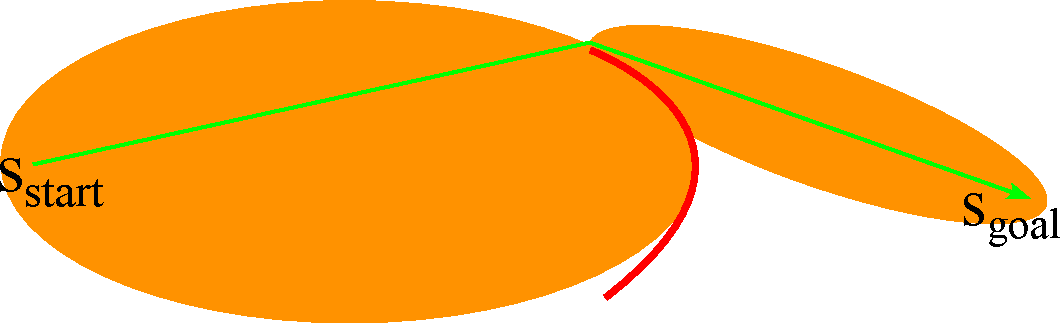
\includegraphics[width=0.8\textwidth]{obrazky-figures/astar-search-space.pdf}
        \medskip
        \rule{0.8\textwidth}{0.4pt}
        \medskip
        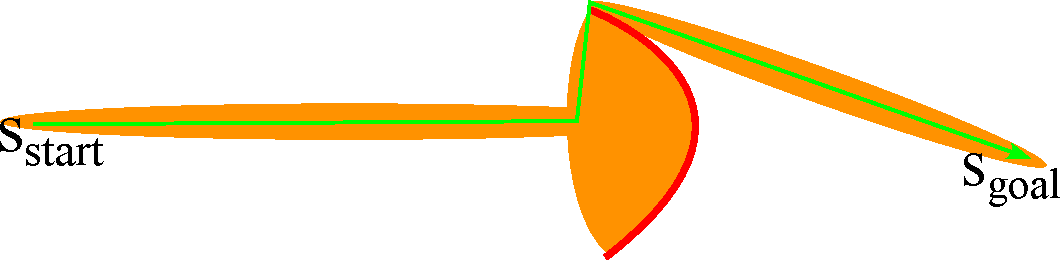
\includegraphics[width=0.8\textwidth]{obrazky-figures/weighted-astar-search-space.pdf}
    \end{center}
    \caption{Porovnání prohledávaných částí stavového prostoru při použití metod \emph{A*} (nahoře) a~\emph{Weighted A*} (dole) \cite{Likachev_astar_weighted_astar}. Oranžová plocha symbolizuje prohledané stavy, zelená šipka nalezenou cestu, červená křivka překážku.}
    \label{fig:astar-wighted-astar-search-space}
\end{figure}

\subsubsection*{Metoda Anytime Repairing A*}

Myšlenka metody \emph{Anytime Repairing A*} (\emph{ARA*}) \cite{ARA_star} spočívá v~rychlém nalezení cesty, která není optimální, a~následném \uv{opravování} této cesty pro získání optimálního výsledku. Metoda opakovaně vykonává průchod stavovým prostorem metodou \emph{Weighted A*} a~při tom postupně snižuje hodnotu $\epsilon$. Hodnoty získané předcházejícími průchody si uchovává pro příští průchody, aby mohly být vykonány rychleji. Jakmile $\epsilon$ dosáhne hodnoty $1$, vykoná se poslední průchod, který již nalezne optimální řešení.

Podobně jako u~\emph{LPA*} a~\emph{D* Lite} se u~této metody hovoří o~tzv. \uv{lokální nekonzistentnosti uzlu}. Uzel $s$ je lokálně nekonzistentní, pokud existuje cesta s~cenou nižší, než je jemu aktuálně přiřazená hodnota $g(s)$.

\emph{ARA*} využívá 3 kolekce: \emph{OPEN}, \emph{CLOSED} a~\emph{INCONS}. Kolekce \emph{OPEN} je typu prioritní fronta a~plní stejnou funkci jako u~metody \emph{A*}: uchovává uzly určené k~expanzi (lokálně nekonzistentní uzly). Kolekce \emph{CLOSED} opět plní stejnou funkci jako u~metody \emph{A*}: uchovává uzly, které již expandovány byly. Na rozdíl od \emph{A*}, u~\emph{ARA*} neexistuje varianta bez kolekce \emph{CLOSED}. Kolekce \emph{INCONS} uchovává všechny lokálně nekonzistentní uzly, které již jsou v~kolekci \emph{CLOSED}. Pokud je při expanzi nějakého uzlu vygenerován uzel, který se již nachází v~kolekci \emph{CLOSED}, je umístěn do kolekce \emph{INCONS}. Na začátku jedné iterace \emph{Weighted A*} musí \emph{OPEN} obsahovat všechny lokálně nekonzistentní uzly. Při první iteraci je to počáteční uzel, při následujících iteracích je to sjednocení kolekcí \emph{OPEN} a~\emph{INCONS}.

Ukončující podmínka u~metody \emph{A*} je situace, kdy je vybrán pro expanzi cílový uzel. Jelikož však metoda \emph{ARA*} používá hodnoty získané během předchozích hledání, cílový uzel se při některém z~hledání nemusí stát lokálně nekonzistentním, a~proto se ani nedostane do kolekce \emph{OPEN}. Jiný úhel pohledu na ukončující podmínku metody \emph{A*} je, že ohodnocení $f(s_{goal})$ cílového uzlu $s_{goal}$ je nejnižší ze všech ohodnocení $f(s)$ uzlů $s$ z~kolekce \emph{OPEN}. Tohoto již je možné u~metody \emph{ARA*} dosáhnout.

\section{Metody hraní her}

Metody popsané v~této sekci se zaměřují na hry, ve kterých proti sobě soupeří dva a~více hráčů proti sobě \cite{AI_Russel_Norvig}. Výsledkem hry může být pouze stav, kdy jeden z~hráčů vyhraje a~ostatní prohrají, nebo remízový stav, kdy nelze určit vítěze ani poraženého. Hráči se postupně střídají v~tom, kdo je na tahu. Metody pro správné fungování také vyžadují, aby prostředí hry bylo deterministické a~plně pozorovatelné. Účelem těchto metod je určit, jakou akci by měl vykonat hráč na tahu.

\subsection*{Metoda Minimax}

Metodu \emph{Minimax} \cite{AI_Russel_Norvig} lze použít pouze při hře 2 hráčů. Metoda předpokládá, že oba dva hráči budou hrát optimálně, tedy že hráč na tahu se bude snažit dostat do stavu hry, který je pro něj nejvýhodnější, zatímco jeho soupeř se bude snažit dostat do stavu hry, který je nejméně výhodný pro hráče na tahu. Z~tohoto důvodu se hráč na tahu označuje jménem \emph{Max} a~jeho soupeř jménem \emph{Min}.

Podobně jako u~ostatních metod řešení úloh, i~zde se na stavový prostor hry (úlohy) nahlíží jako na vyhledávací strom, kdy kořenem je aktuální stav hry, hrany jsou akce vykonané hráčem a~listové uzly jsou konečné stavy hry, tj. výhra, prohra nebo remíza. U~většiny her by však bylo příliš náročné procházet celý stavový prostor a~hledat optimální řešení. Proto je typickou úpravou metody omezení maximální hloubky stromu. Listovým uzlem pak mohou být navíc uzly, které se nachází v~maximální hloubce.

Základem metody je funkce \emph{Minimax}, které je předán uzel $n$ a~funkce spočítá jeho ohodnocení. Hráč na tahu ji zavolá pro všechny možné stavy, do kterých se může z~aktuálního stavu dostat, a~poté vykoná akci, která vede do stavu s~nejvyšším ohodnocením. Funkce vypadá následovně:\enlargethispage{-1\baselineskip} % Keep the list items together
\begin{enumerate}
    \item Pokud je uzel $n$ listem, vrať ohodnocení tohoto uzlu.
    \item Pokud je na tahu hráč \emph{Max}, zavolej rekurzivně \emph{Minimax} pro všechny bezprostřední následníky uzlu $n$ a~vrať \emph{nejvyšší} ze získaných ohodnocení.
    \item Pokud je na tahu hráč \emph{Min}, zavolej rekurzivně \emph{Minimax} pro všechny bezprostřední následníky uzlu $n$ a~vrať \emph{nejnižší} ze získaných ohodnocení.
\end{enumerate}

Lze si všimnout, že fungování této metody se velmi podobá metodě \emph{DLS} (bez omezení hloubky stromu metodě \emph{DFS}). Obě metody expandují vždy ty uzly, které se v~rámci vyhledávacího stromu nachází nejhlouběji. Tím pádem jsou i~jejich ohodnocení podobná: pro vyhledávací strom s~faktorem větvení $b$ a~maximální hloubkou $d$ je časová složitost algoritmu $O(b^m)$ a~prostorová složitost $O(b \cdot m)$. Časovou složitost lze dále optimalizovat pomocí tzv. \emph{alfa-beta řezů}.

\subsection*{Alfa-beta řezy}

Časová složitost metody \emph{Minimax} roste exponenciálně s~rostoucí maximální hloubkou vyhledávacího stromu \cite{AI_Russel_Norvig}. Ačkoliv není možné se úplně zbavit exponentu, je možné jej snížit až na polovinu. Toho lze dosáhnout ignorováním uzlů, u~kterých víme, že na ohodnocení rodičovského uzlu nebudou mít vliv.

Příklad takových zbytečně vyšetřovaných uzlů je ukázán na obrázku~\ref{fig:alpha-beta-pruning}. Soustřeďme se na uzel označený písmenem \emph{B}. Na tahu je zde hráč \emph{Max}, tudíž hledáme nejvyšší možné ohodnocení. Při vyšetřování jeho levého podstromu bylo zjištěno, že jeho ohodnocení je 5. Při vyšetřování jeho pravého podstromu byla nalezena hodnota 4. Vzhledem k~tomu, že na tahu je v~kořeni tohoto podstromu hráč \emph{Min} a~vybírá si nejnižší možné ohodnocení, víme, že hodnota tohoto podstromu bude $\leq 4$. Tato hodnota je už nyní nižší než ohodnocení levého podstromu (5), a~tedy není nutné tento podstrom dále vyšetřovat. Ještě zajímavější je vyšetřování uzlu \emph{C}. Bylo zjištěno, že ohodnocení jeho rodiče (uzlu \emph{A}) může dosáhnout až hodnoty 6. Při vyšetřování levého podstromu uzlu \emph{C} byla vrácena hodnota 5. Jelikož je v~tomto uzlu na tahu hráč \emph{Min}, už teď víme, že jeho ohodnocení nebude vyšší než 5. V~uzlu \emph{A} je však na tahu hráč \emph{Max} a~hledá ohodnocení vyšší než 6, proto celý pravý podstrom uzlu \emph{C} může být ignorován.

\begin{figure}[ht]
    \centering
    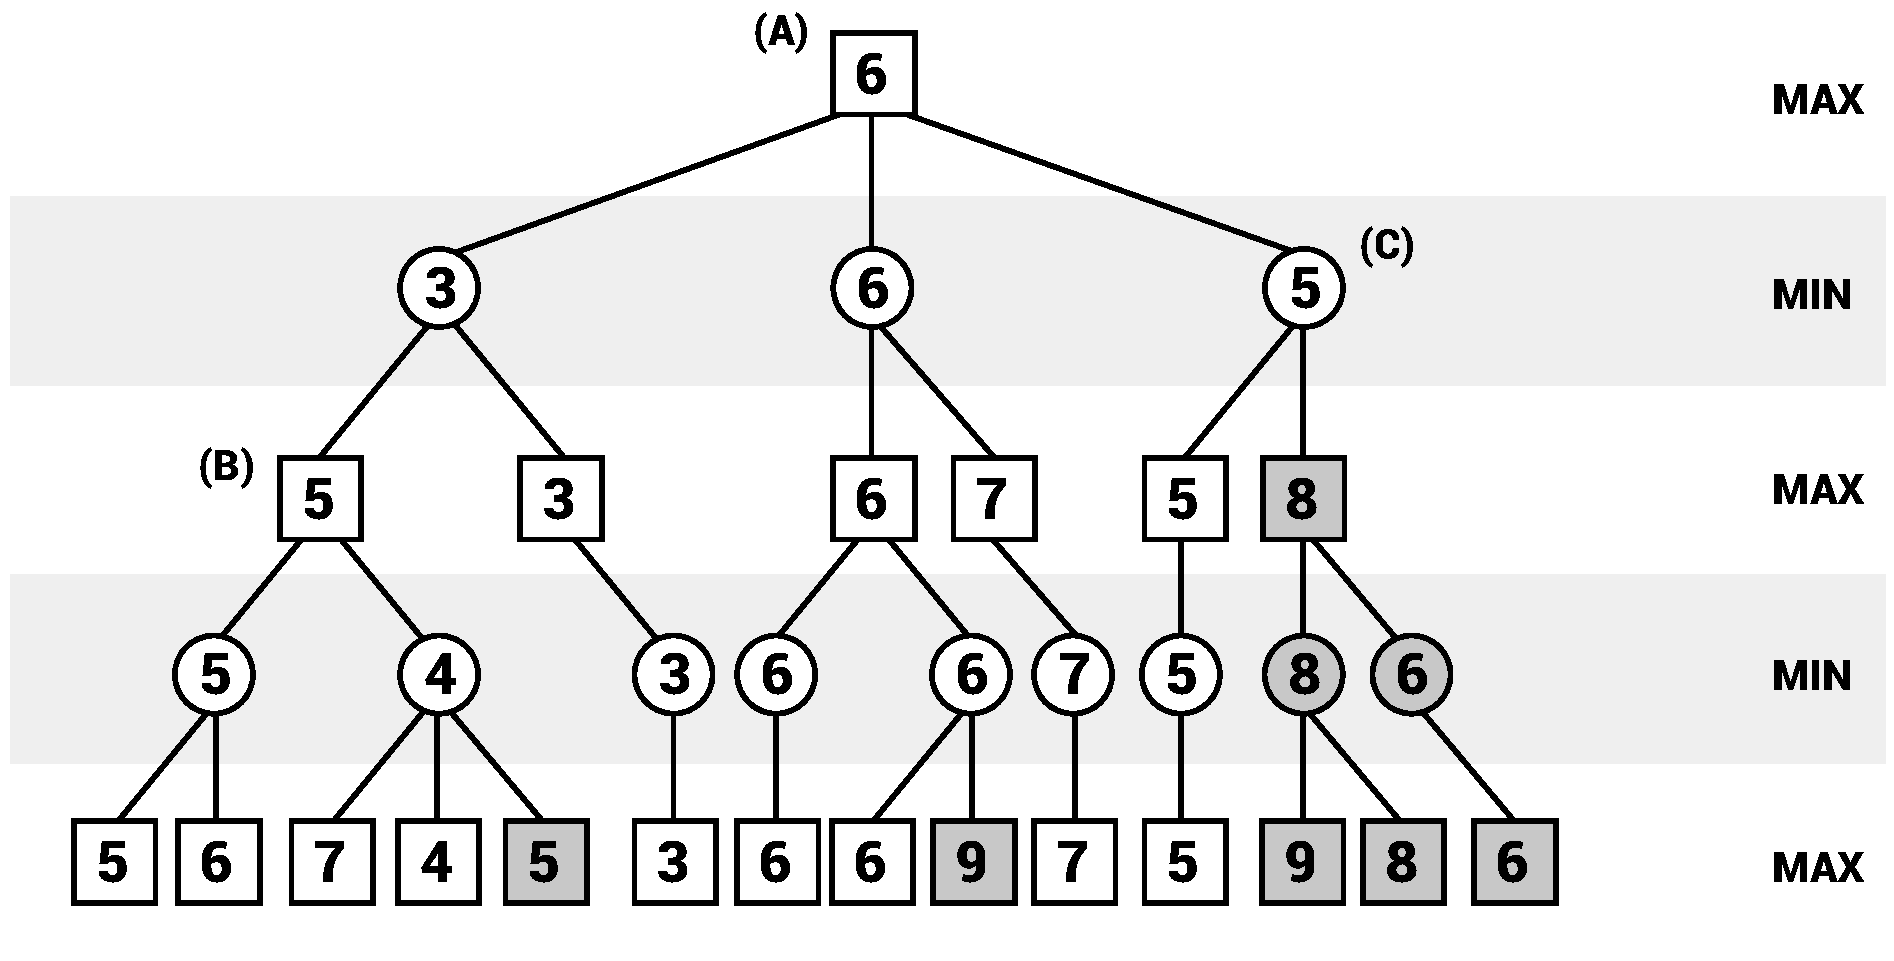
\includegraphics[width=0.8\textwidth]{obrazky-figures/ab-pruning.pdf}
    \caption{Příklad vyhledávacího stromu \cite{ab_pruning} sestaveného metodou \emph{Minimax}. Čísla v~uzlech udávají jejich ohodnocení. Šedě zbarvené uzly jsou vyšetřovány zbytečně.}
    \label{fig:alpha-beta-pruning}
\end{figure}

Účelem \emph{alfa-beta řezů} je předejít tomuto zbytečnému vyšetřování uzlů. Metoda každému uzlu přiřadí proměnné $\alpha$ a~$\beta$, které se inicializují na hodnoty $-\infty$ a~$\infty$ v~tomto pořadí a~následně se modifikují před a~po rekurzivních voláních funkce \emph{Minimax}. Jakmile nastane situace $\alpha \geq \beta$, provede se \uv{řez} (\uv{alfa řez} nebo \uv{beta řez}) a~ostatní následníci uzlu, v~němž nastal tento \uv{řez} nebudou vyšetřováni. Funkce \emph{Alfa-beta} (tj. \emph{Minimax} po zavedení \emph{alfa-beta řezů}) vypadá následovně:
\begin{enumerate}
    \item Pokud je uzel $n$ listem, vrať ohodnocení tohoto uzlu.
    \item Pokud je na tahu hráč \emph{Max}, pak:
    \begin{enumerate}
        \item Dokud platí $\alpha < \beta$, volej rekurzivně funkci \emph{Alfa-beta} pro každého bezprostředního následníka uzlu $n$ s~aktuálními hodnotami $\alpha$ a~$\beta$. Pokud je vrácená hodnota \emph{vyšší} než aktuální hodnota proměnné $\alpha$, nastav hodnotu proměnné $\alpha$ na tuto vrácenou hodnotu.
        \item Pokud $\alpha \geq \beta$ (alfa řez) nebo všichni bezprostřední následníci uzlu $n$ již byli prozkoumáni, vrať aktuální hodnotu proměnné $\alpha$.
    \end{enumerate}
    \item Pokud je na tahu hráč \emph{Min}, pak:
    \begin{enumerate}
        \item Dokud platí $\alpha < \beta$, volej rekurzivně funkci \emph{Alfa-beta} pro každého bezprostředního následníka uzlu $n$ s~aktuálními hodnotami $\alpha$ a~$\beta$. Pokud je vrácená hodnota \emph{nižší} než aktuální hodnota proměnné $\beta$, nastav hodnotu proměnné $\beta$ na tuto vrácenou hodnotu.
        \item Pokud $\alpha \geq \beta$ (beta řez) nebo všichni bezprostřední následníci uzlu $n$ již byli prozkoumáni, vrať aktuální hodnotu proměnné $\beta$.
    \end{enumerate}
\end{enumerate}

Jak již bylo zmíněno, časová ani prostorová složitost se zavedením \emph{alfa-beta řezů} nezmění. V~ideálním případě je však možné snížit počet vyšetřovaných uzlů z~$b^m$ na $b^\frac{m}{2}$. Znamená to, že při použití \emph{alfa-beta řezů} můžeme prohledávat téměř $2\times$ hlubší strom než u~obyčejného \emph{Minimax} a~využít při tom stejné množství času. Onoho ideálního případu je ale velmi obtížné dosáhnout; skutečný počet vyšetřovaných uzlů se pak bude typicky pohybovat okolo hodnoty $b^{\frac{3}{4}m}$.

\subsection*{Metoda Max\textsuperscript{n}}

Metodu \emph{Minimax} nelze použít u~her, které hrají více než 2 hráči. Pro tento účel je nutné tuto metodu upravit. Tato upravená metoda bývá nazývána \emph{Max\textsuperscript{n}} \cite{Maxn}.

U~metody \emph{Minimax} pro hodnocení stavu hry stačila pouze jedna hodnota. Hráč \emph{Max} usiloval o~to, aby tato hodnota byla co největší, zatímco hráč \emph{Min} o~to, aby byla co nejmenší. U~metody \emph{Max\textsuperscript{n}} se každý hráč snaží dosáhnout hodnocení stavu hry, které je nejvýhodnější pro něj samotného. Proto místo jedné hodnoty využívá tato metoda vektor hodnot $(v_1, v_2, \ldots, v_n)$, kde $n$ je počet hráčů a~hodnota $v_i$ je ohodnocení daného stavu z~pohledu hráče $i$. Například, hrají-li hru 3 hráči a~ohodnocení stavu je dáno vektorem $(8, 2, 5)$, znamená to, že pro hráče 1 má tento stav hodnotu 8, pro hráče 2 hodnotu 2 a~pro hráče 3 hodnotu 5.

Základem metody je opět stejnojmenná funkce, \emph{maxn}, která je volána rekurzivně. Je jí předán uzel $n$, pro který funkce spočítá ohodnocení. Návratovou hodnotou je vektor ohodnocení daného uzlu, ve kterém každá hodnota přísluší právě jednomu hráči. Funkce vypadá následovně:
\begin{enumerate}
    \item Pokud je uzel $n$ listem, vrať ohodnocení tohoto uzlu.
    \item Pokud je na tahu hráč $i$, zavolej rekurzivně \emph{maxn} pro všechny bezprostřední následníky uzlu $n$ a~vrať ohodnocení, jehož $i$-tá složka je nejvyšší ze všech.
\end{enumerate}
Příklad průběhu metody je znázorněn na obrázku~\ref{fig:maxn}.

\begin{figure}[ht]
    \centering
    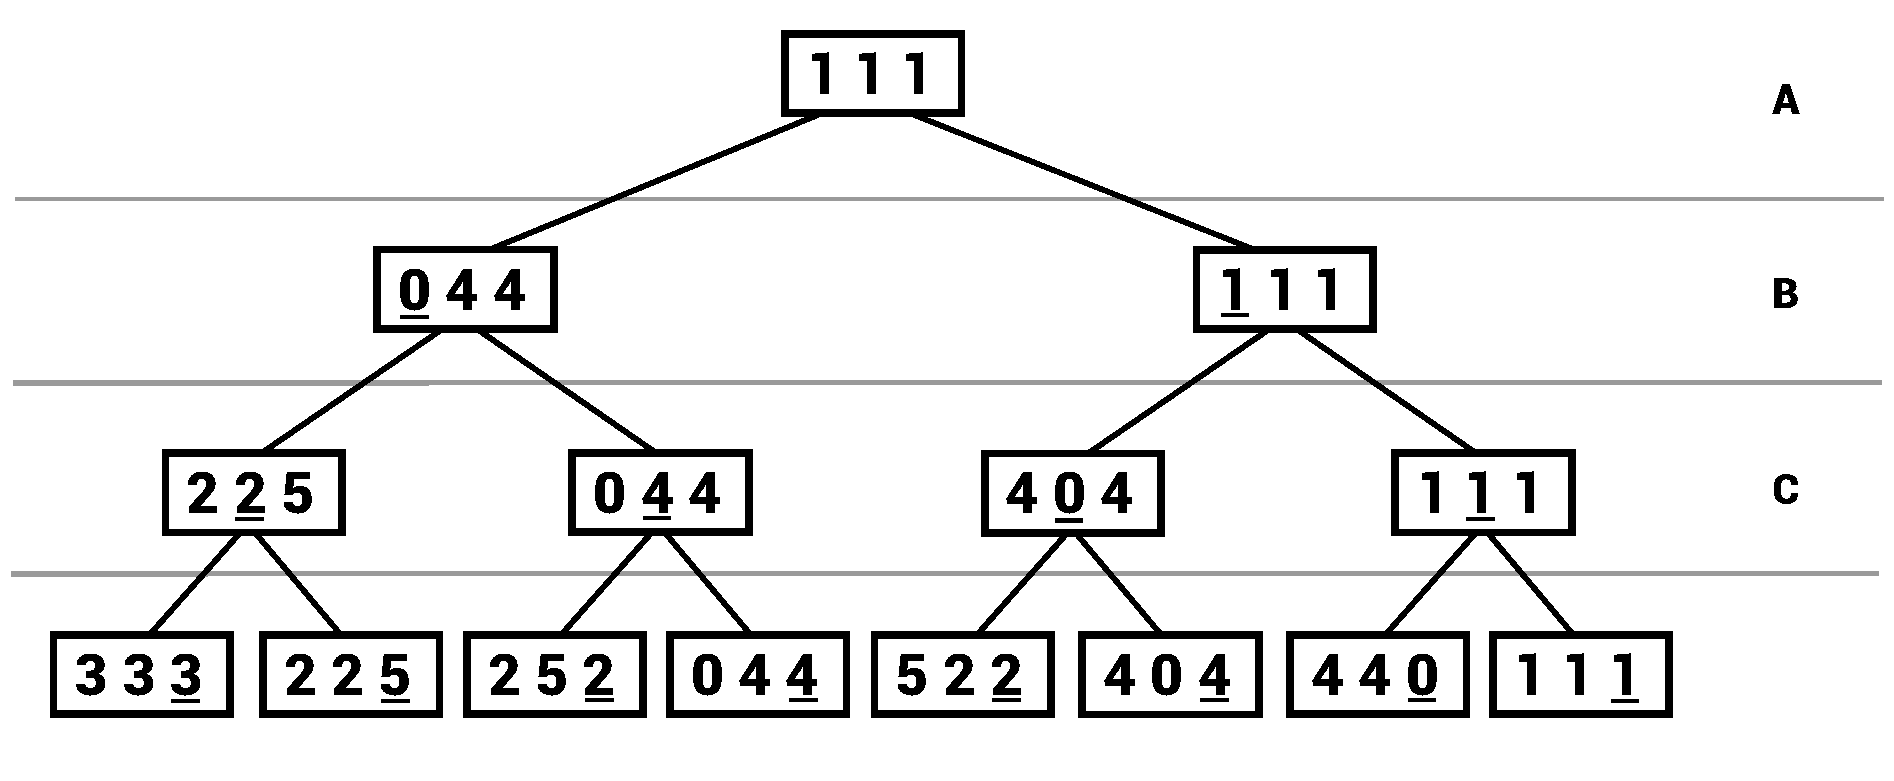
\includegraphics[width=0.8\textwidth]{obrazky-figures/maxn.pdf}
    \caption{Příklad použití metody \emph{Max\textsuperscript{n}}. Čísla v~uzlech představují ohodnocení stavu pro hráče A, B a~C v~tomto pořadí. Podtržená čísla jsou ohodnocení, která jsou porovnávána při výběru nejlepšího uzlu. Příklad byl převzat z~\cite{Maxn}.}
    \label{fig:maxn}
\end{figure}

Časová složitost metody je opět exponenciální $O(b^m)$ \cite{Search_policies_in_multiplayer_games_Nijssen_Winands}. Nicméně, počet výpočtů ohodnocení stavů závisí také na počtu hráčů $n$, proto metoda bude vždy počítat okolo $nb^m$ ohodnocení stavů \cite{Maxn}. Některým těmto výpočtům lze však předejít metodou zvanou \emph{Shallow pruning}.

\subsection*{Shallow pruning}

\emph{Shallow pruning} \cite{Maxn}, stejně jako \emph{alfa-beta řezy} u~metody \emph{Minimax}, předchází nadbytečnému vyhodnocování některých hodnot metodou \emph{Max\textsuperscript{n}}. Tyto řezy bohužel nemohou ignorovat celé podstromy, jak tomu bylo u~\emph{alfa-beta řezů}, ale alespoň předchází výpočtům některých složek ohodnocení stavů.

Funkce \emph{pmaxn}, která je upravenou variantou funkce \emph{maxn}, vrací pouze jednu složku z~ohodnocení stavu a~to tu, která je použita pro porovnání v~rodičovském uzlu. Dále také vrací ukazatel na \emph{listového} potomka, kterému toto ohodnocení náleží. Pokud se vrácené ohodnocení dostane do vyšší úrovně vyhledávacího stromu, lze ukazatel na potomka využít pro vypočítání jiných složek ohodnocení stavu. Funkce vypadá takto:
\begin{enumerate}
    \item Pokud je uzel $n$ listem a~v~uzlu, který je bezprostředním předchůdcem uzlu $n$, je na tahu hráč $i$, vrať $i$-tou složku ohodnocení uzlu $n$ a~ukazatel na tento uzel.
    \item Jinak:
    \begin{enumerate}
        \item Zavolej rekurzivně \emph{pmaxn} pro každého bezprostředního následníka uzlu $n$. Najdi volání, které vrátilo nejvyšší ohodnocení, a~ulož si uzel $n^*$, kterému toto ohodnocení náleží.
        \item Pokud v~uzlu, který je bezprostředním předchůdcem uzlu $n$, je na tahu hráč $i$, vrať $i$-tou složku ohodnocení uzlu $n^*$ a~ukazatel na tento uzel.
    \end{enumerate}
\end{enumerate}

Časová složitost metody zůstává stále exponenciální $O(b^m)$, avšak skutečný počet výpočtů ohodnocení stavů je oproti \emph{Max\textsuperscript{n}} bez použití řezů nižší: přibližně
\begin{equation}
    \frac{b^{m+1} - b^{m-n+1}}{b-1}
\end{equation}
Pro odvození tohoto vztahu viz \cite{Maxn}. Účinnost metody je znázorněna na obrázku~\ref{fig:maxn-shallow-pruning}.

\begin{figure}[ht]
    \centering
    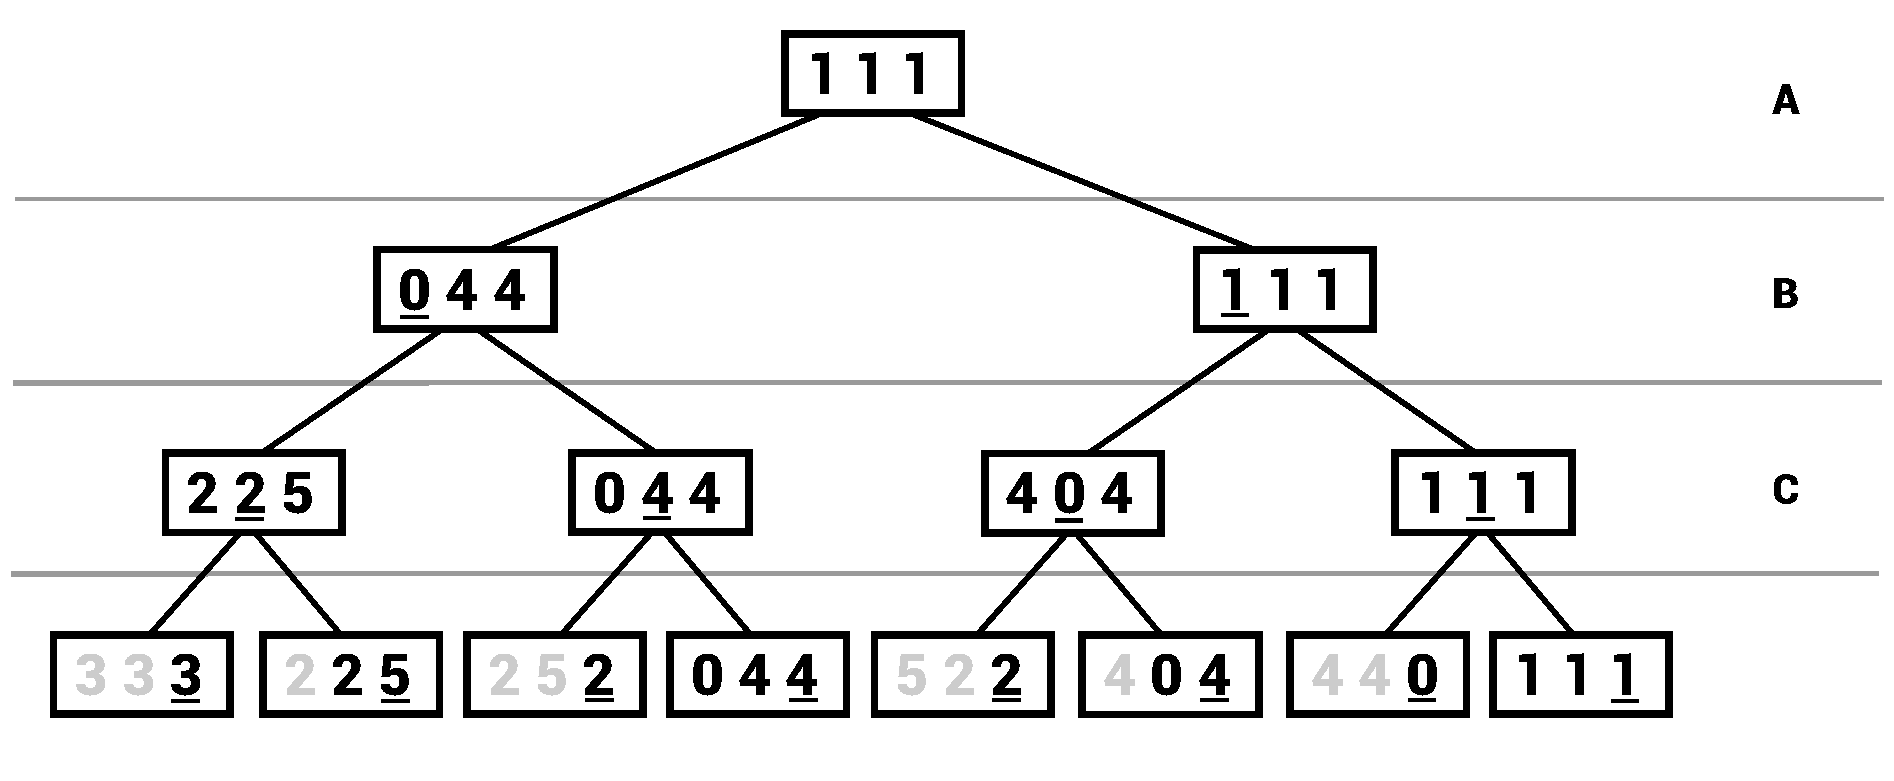
\includegraphics[width=0.8\textwidth]{obrazky-figures/maxn-shallow-pruning.pdf}
    \caption{Ukázka účinnosti metody \emph{Shallow pruning} \cite{Maxn}. Stavový prostor je stejný, jako na obrázku~\ref{fig:maxn}, ale šedě zbarvená ohodnocení byla metodou \uv{ořezána}. (Ořezání je uvedeno pouze v~nejnižší vrstvě; ačkoliv metoda provádí výpočty i~ve vyšších vrstvách, jsou de facto prováděny pouze nad listovými uzly a~do vyšších vrstev se pouze propagují.)}
    \label{fig:maxn-shallow-pruning}
\end{figure}


\chapter{Představení hry}
\label{ch:predstaveni-hry}

Tato kapitola se věnuje popisu výsledné aplikace. Obsahuje popis samotné hry \emph{Bubble Brawl} a~její pravidla. Dále je zde uvedena interakce mezi uživatelem a~aplikací\,--\,ovládání, navigace mezi pohledy. Také je zde představen vestavěný editor herní plochy.

\section{Pravidla}

Hra \emph{Bubble Brawl} je typu \uv{battle royale}. Jejím cílem je tedy eliminovat všechny protivníky a~zůstat poslední naživu. Hráči ovládají kruhové entity nazývané \uv{bubliny} (\uv{bubbles}) ve 2rozměrném labyrintu. 

Hra umožňuje hráčům svislý, vodorovný i~diagonální pohyb. Překážky v~labyrintu jsou vyznačeny polygony, skrz které hráči nemohou procházet. Kromě toho představuje herní plocha obdélníkový box, který taktéž není možné opustit. Mimo pohybu je možné změnit stav bubliny tím, že hráč (manuálně) zmenší její velikost. Tato možnost existuje z~důvodu, aby bylo možné projít úzkými chodbami, pro které je bublina příliš velká. Důsledkem však je, že hráč takto ztratí body života (viz následující odstavec), nicméně nelze takto ztratit poslední bod života.

Hráči začínají s~určitým množstvím bodů života a~zůstávají ve hře, dokud je toto množství větší než 0. Když se 2 a~více hráčů dotýká, všichni dotýkající se hráči ztrácí body života. Kromě toho na této veličině závisí několik dalších vlastností hráče:
\begin{itemize}
    \item Velikost\,--\,poloměr hráčovy bubliny (přímo úměrně),
    \item Rychlost pohybu (nepřímo úměrně),
    \item Síla\,--\,kolik bodů života ubírá hráč svým protivníkům (přímo úměrně).
\end{itemize}

V~průběhu hry se v~náhodných intervalech objevují na herní ploše bonusy ve tvaru kruhu, které hráčům doplňují body života. Aby byl bonus na hráče aplikován, musí se bonus s~bublinou hráče navzájem dotýkat. Následkem toho tento bonus zmizí a~žádný jiný hráč ho poté už nemůže použít. Místo, kde se bonus objeví je náhodné. Nikdy však nemůže kolidovat s~překážkou. Navíc, v~jeden okamžik může být na herní ploše pouze jeden bonus. Množství života získané z~bonusu je také náhodně vybráno ze 4~možných hodnot relativních vůči počátečnímu množství života: $25\,\%$, $50\,\%$, $75\,\%$ a~$100\,\%$.

\section{Uživatelské rozhraní}
\label{sec:uzivatelske-rozhrani}

Aplikace se skládá z~běžných grafických komponent, jako jsou tlačítka, přepínače (\uv{\emph{radio button}}) nebo rozbalovací seznamy. Uživatel s~nimi interaguje převážně pomocí myši. Vstup z~klávesnice je použit téměř výhradně pro samotnou hru.

\subsection*{Navigace}

Po spuštění aplikace se uživateli zobrazí logo a~následně hlavní nabídka se 3 tlačítky. Tlačítko \uv{Play} zobrazí plochu pro nastavení hry. Tlačítko \emph{Stage editor} otevře editor herní plochy. Editor je popsán v~kapitole~\ref{sec:editor-herni-plochy}. Poslední tlačítko \uv{Quit} zavře aplikaci.

Uživatel musí před spuštěním hry provést nastavení hry (viz obrázek~\ref{fig:game-setup}). Nastavení sestává z~výběru herní plochy, na níž se bude hra hrát, určení počtu hráčů a~jejich typů.

\begin{figure}[ht]
    \centering
    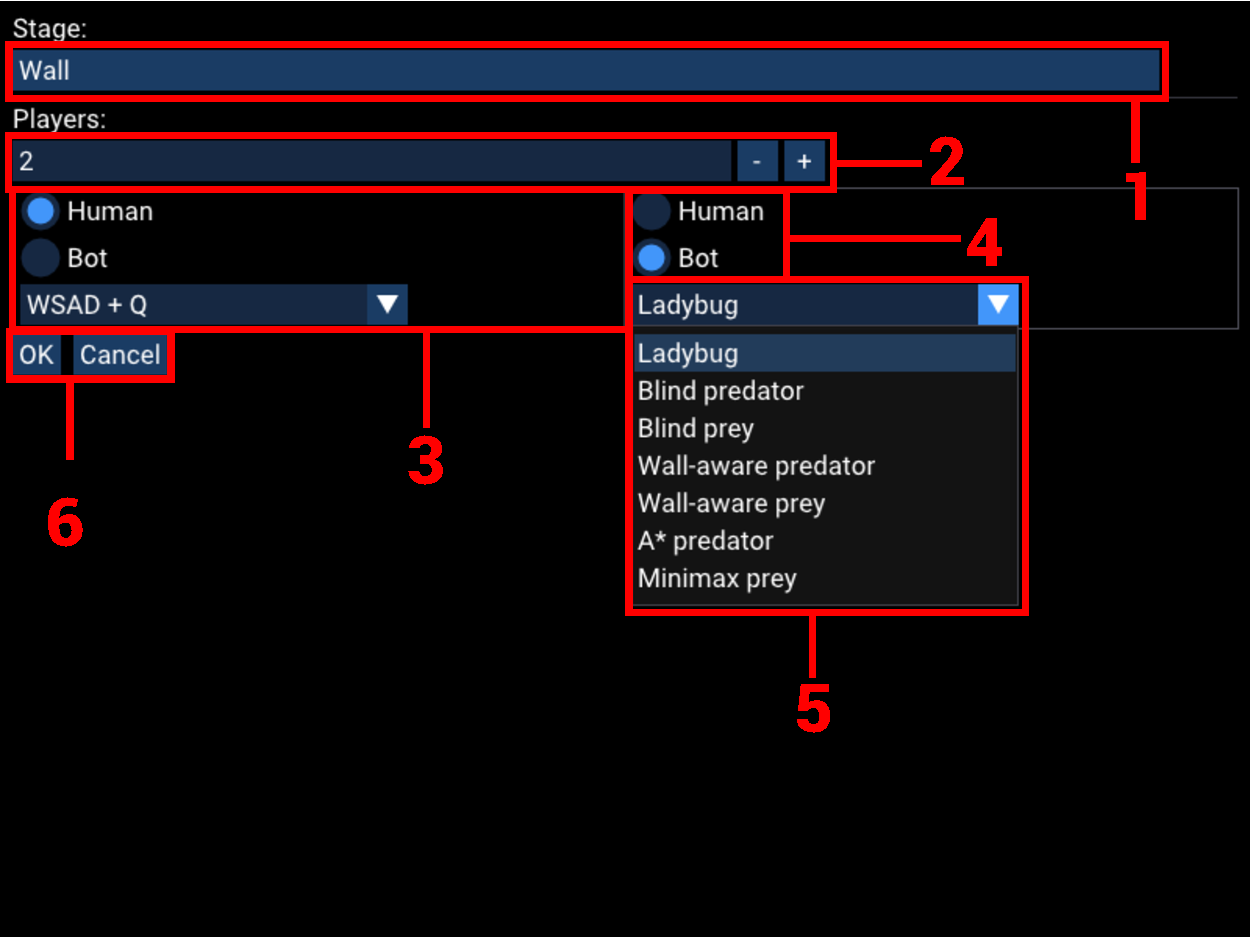
\includegraphics[width=0.8\textwidth]{obrazky-figures/game-setup.pdf}
    \caption{Plocha pro nastavení hry. Tlačítko (1) umožňuje výběr herní plochy. Textové pole (2) umožňuje nastavit počet hráčů. Panel (3) seskupuje nastavení týkající se konkrétního hráče a~obsahuje přepínače (4) pro výběr typu hráče a~rozbalovací seznam (5) pro výběr ovládání hráče. Pomocí tlačítek (6) lze spustit hru nebo vrátit se zpět na hlavní nabídku.}
    \label{fig:game-setup}
\end{figure}

Po kliknutí na tlačítko označené popiskem \uv{Stage:} se zobrazí seznam existujících herních ploch. Uživatel zde může vybrat nějakou položku ze seznamu nebo se tlačítkem \uv{Cancel} vrátit zpět na plaochu nastavení hry bez výběru herní plochy.

Pokud je nějaká herní plocha vybrána, může uživatel nastavit počet hráčů ve hře pomocí textového pole \uv{Players:}. Maximální hodnota tohoto pole je rovna maximálnímu počtu hráčů, který na vybrané herní ploše může hrát.

S~měnící se hodnotou v~tomto poli se také mění počet panelů pro nastavení jednotlivých hráčů. V~těchto panelech se nachází přepínače, kde hráč může vybrat typ hráče: člověk (\uv{Human}) nebo počítač (\uv{Bot}). Na základě vybraného typu hráče se mění funkce rozbalovacího seznamu: pokud uživatel vybral přepínač \uv{Human}, rozbalovací seznam slouží pro výběr kláves, pomocí kterých bude hráč ovládat svoji \uv{bublinu}. Pokud uživatel vybral přepínač \uv{Bot}, pak rozbalovací seznam bude obsahovat různé typy těchto \uv{botů}. Umělé inteligenci se věnuje kapitola~\ref{sec:entity-rizene-pocitacem}. Zde se pouze zmíním o~tom, že typ \uv{Ladybug} se pohybuje čistě náhodně, typ \uv{Predator} se snaží vždy útočit a~\uv{Prey} se snaží vždy utíkat.

Pokud bylo vše vyplněno správně, je možné tlačítkem \uv{OK} spustit hru. V~opačném případě bude tlačítko zašedlé a~nepůjde na něj kliknout. Aby bylo možné spustit hru, musí být vybrána herní plocha a~nesmí být 2 různí hráči typu \uv{Human}, kteří jsou ovládáni stejnými klávesami. Není však problém, pokud počet hráčů je 0 nebo 1; v~tomto případě hra ihned po spuštění skončí. Z~plochy nastavení hry je možné se kdykoliv vrátit zpět na hlavní nabídku pomocí tlačítka \uv{Cancel}.

\subsection*{Probíhající hra}

Plocha, na níž je zobrazen aktuální stav hry, je rozdělena na 2 části: herní plochu a~boční panel (viz obrázek~\ref{fig:in-game}). Herní plocha zobrazuje aktuální stav hry\,--\,hráče, překážky a~bonusy. Hráči jsou na herní ploše vyznačeni pomocí barevných kruhů, přičemž každému hráči patří jiná barva. Překážky včetně ohraničení herní plochy jsou znázorněny šedými polygony. Bonusy jsou světle modré kruhy s~červeným ohraničením a~červeným symbolem \uv{plus} uprostřed. Po sebrání se bonus změní na text informující o~tom, jaké množství života hráč z~bonusu získal.

\begin{figure}[ht]
    \centering
    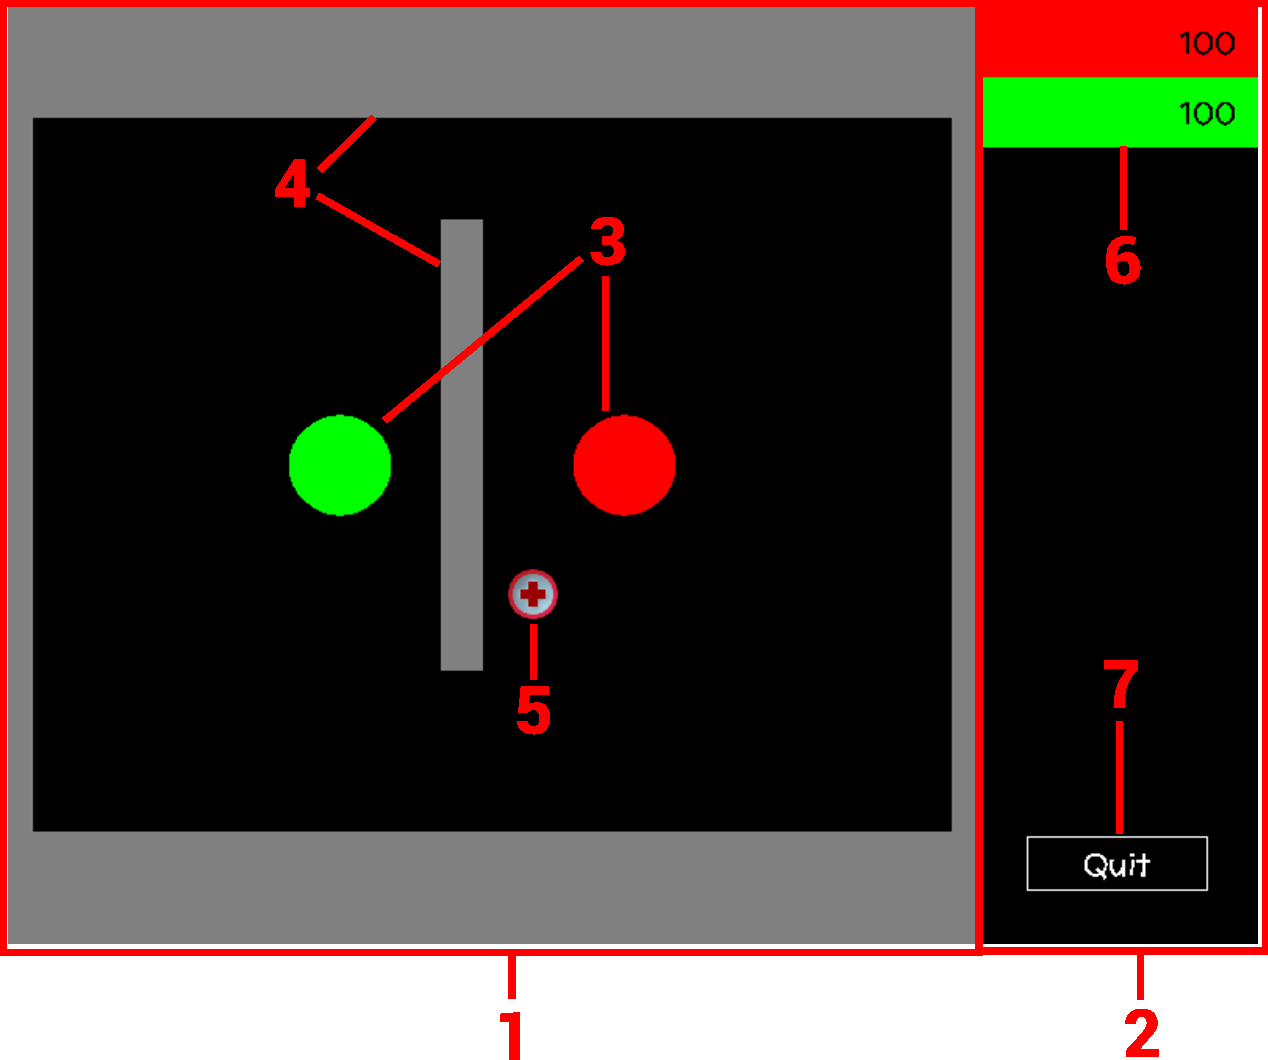
\includegraphics[width=0.8\textwidth]{obrazky-figures/in-game.pdf}
    \caption{Plocha s~probíhající hrou. Plocha je rozdělena na herní plochu (1) a~boční panel (2). Na herní ploše se zobrazují herní objekty\,--\,hráči (3), překážky (4) a~bonusy (5). V~bočním panelu se nachází počítadla množství života hráčů (6) a~tlačítko pro ukončení hry (7).}
    \label{fig:in-game}
\end{figure}

Boční panel je umístěn vpravo. V~jeho horní části se nachází počítadla množství života hráčů, jejichž barvy odpovídají barvám hráčů. Jakmile je nějaký hráč vyřazen ze hry, jeho počítadlo je skryto. Hru je možné kdykoliv ukončit tlačítkem \uv{Quit} v~dolní části bočního panelu.

Jakmile zůstal ve hře pouze 1 hráč, zobrazí se uprostřed herní plochy nápis \uv{WINNER} (\uv{vítěz}). Pokud nastane situace, že na herní ploše není ani jeden hráč, zobrazí se místo toho nápis \uv{DRAW GAME} (\uv{remíza}). Hra i~potom pokračuje dál; bonusy se na herní ploše dále objevují a~hráč, pokud je nějaký naživu, se může po herní ploše volně pohybovat.

\section{Editor herní plochy}
\label{sec:editor-herni-plochy}

Uživatel má možnost vytvářet vlastní herní plochy pomocí vestavěného editoru. Editor lze spustit z~hlavního menu tlačítkem \uv{Stage editor}.

Editor herní plochy se skládá z~menu, panelu nástrojů a~pracovní plochy, viz obrázek~\ref{fig:stage-editor}. V~menu se nachází tlačítka pro načítání a~ukládání herní plochy, dále tlačítka pro krok zpět a~vpřed (\uv{Undo} a~\uv{Redo}) a~vpravo tlačítko pro návrat do hlavního menu. Panel nástrojů obsahuje nástroje, které slouží pro manipulaci s~objekty na herní ploše. Pracovní plocha slouží pro samotné sestavování herní plochy.

\begin{figure}[ht]
    \centering
    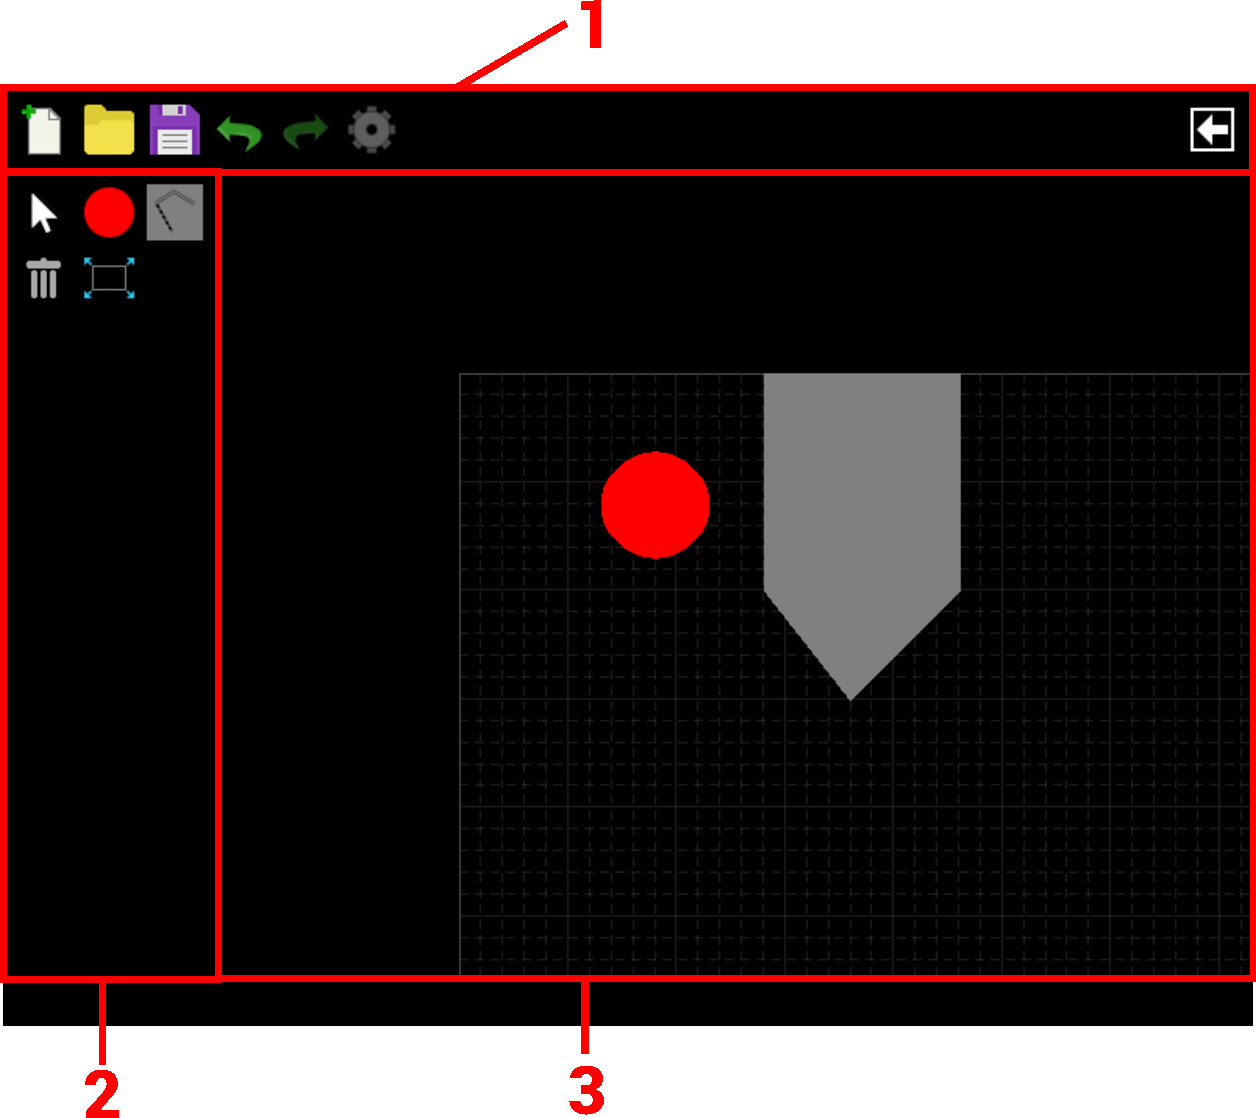
\includegraphics[width=0.8\textwidth]{obrazky-figures/stage-editor.pdf}
    \caption{Editor herní plochy. Skládá se z~menu (1), panelu nástrojů (2) a~pracovní plochy (3).}
    \label{fig:stage-editor}
\end{figure}

% Describe editor button
% Parameters:
%  #1 Button name
%  #2 Path to button image
%  #3 Button description
\newcommand{\describeeditorbutton}[3]{
\noindent\begin{tabularx}{\textwidth}{lX}
    \scalebox{2}{\includegraphics[valign=b]{#2}} & \textbf{#1}\,--\,#3 \\
    \\
\end{tabularx}
}

Následují vysvětlivky jednotlivých tlačítek. Obrázky tlačítek byly převzaty přímo z~výsledné aplikace.\\

\describeeditorbutton{New}{obrazky-figures/new.png}{Vytvoří novou, prázdnou herní plochu.}

\describeeditorbutton{Open}{obrazky-figures/open.png}{Zobrazí seznam existujících herních ploch. Po kliknutí na některou z~položek tohoto seznamu nahraje vybranou herní plochu ze souboru.}

\describeeditorbutton{Save}{obrazky-figures/save.png}{Uloží rozpracovanou herní plochu do souboru. Pokud k této ploše není přiřazen žádný soubor (nebyla načtena ze souboru a ani zatím nebyla ukládána), vytvoří se nový soubor. Jeho název bude vybrán podle pravidel popsaných níže.}

\describeeditorbutton{Undo}{obrazky-figures/undo.png}{Vrátí se zpět do stavu před poslední vykonanou akcí. Opakovaným stiskem tohoto tlačítka se lze vrátit do stavu před vykonáním více než jedné akce.}

\describeeditorbutton{Redo}{obrazky-figures/redo.png}{Opakuje poslední akci vrácenou pomocí tlačítka \uv{Undo}. Pokud zatím nebylo provedeno \uv{undo}, nebo od jeho posledního vykonání byla provedena jiná akce, nestane se nic. Opakovaným stiskem tohoto tlačítka lze opakovat více než jednu vrácenou akci.}

\describeeditorbutton{Stage properties}{obrazky-figures/cogwheel.png}{Umožňuje změnit vlastnosti týkající se herní plochy. Zobrazí se okno s~textovou kolonkou, kde má uživatel možnost změnit název herní plochy. Pod kolonkou je zobrazen název souboru, do kterého bude herní plocha uložena při dalším stisku tlačítka \uv{Save}.}

\describeeditorbutton{Select tool}{obrazky-figures/select-tool.png}{Umožňuje přesouvat a~upravovat již existující objekty na herní ploše. Objekt je nejdříve nutné vybrat kliknutím. Lze také vybrat více objektů přidržením klávesy \texttt{Shift} a~následně přesunout všechny vybrané objekty najednou. Při přesouvání je nutné dodržovat pravidla uvedená u~jednotlivých nástrojů pro objekty níže, jinak nebude přesun proveden.}

\describeeditorbutton{Player tool}{obrazky-figures/player-tool.png}{Umožňuje přidávat na herní plochu objekty hráčů. Přidané objekty nesmí kolidovat s~objekty překážek, jiných hráčů, ani nesmí zasahovat mimo hranice herní plochy, jinak nebude objekt na herní plochu přidán. Pokud je vybrán tento nástroj, zobrazí se na pozici kurzoru myši bílá přerušovaná kružnice. Není-li možné na danou pozici objekt hráče umístit, kružnice zčervená.}

\describeeditorbutton{Obstacle tool}{obrazky-figures/obstacle-tool.png}{Umožňuje konstruovat objekty překážek na herní ploše. Konstrukce překážky probíhá přidáváním jednotlivých vrcholů na herní plochu a~následným uzavřením objektu stiskem pravého tlačítka myši. Nově přidané hrany se nesmí překrývat s~existujícími hranami konstruovaného objektu, ani s~objekty hráčů. Nicméně, dvě a~více překážek se smí překrývat. Pokud byl na pracovní plochu umístěn alespoň jeden vrchol a~překážka zatím nebyla uzavřena, zobrazí se mezi všemi propojenými body plná šedá čára a~mezi posledním bodem a~kurzorem myši čára přerušovaná. Není-li možné na danou pozici umístit vrchol, přerušovaná čára zčervená. Změna aktivního nástroje během konstruování překážky způsobí přerušení konstruování.}

\describeeditorbutton{Delete tool}{obrazky-figures/trash-can.png}{Umožňuje mazat objekty na herní ploše. Pokud byly nějaké objekty vybrány pomocí nástroje \uv{Select tool}, pak při kliknutí na některý z~vybraných objektů budou odstraněny všechny vybrané objekty. Pokud není vybrán žádný objekt, odstraní se pouze ten, na který uživatel klikl.}

\describeeditorbutton{Resize stage tool}{obrazky-figures/resize.png}{Umožňuje měnit velikost herní plochy přetažením jejího pravého dolního rohu. Při změně velikosti nesmí dojít k~tomu, aby některý z~hráčů zasahoval mimo hranice herní plochy, jinak nebude změna provedena.}

Uživatel nemá možnost vybírat si název souboru s~herní plochou. Soubory jsou vždy ukládány do adresáře \uv{\texttt{stage/}}. Pokud nebyla herní plocha načtena ze souboru, název souboru je vygenerován podle názvu herní plochy tímto způsobem:
\begin{enumerate}
    \item Všechna velká písmena se změní na malá. Všechny mezery se změní na podtržítka.
    \item Vyjmou se všechny nealfanumerické znaky, které nejsou podtržítka.
    \item Pokud název přesahuje 28 znaků, přebývající znaky na konci řetězce se odstraní.
    \item Pokud je název prázdný řetězec, použije se výchozí \uv{stage}.
    \item Pokud již v~adresáři \texttt{stage/} existuje soubor se stejným názvem, připojí se na konec názvu souboru číslo \uv{1}. Pokud i~tento soubor již existuje, číslo se zvyšuje do té doby, než je nalezen unikátní název.
\end{enumerate}
Soubor je následně možné manuálně přejmenovat; tedy není nutné, aby název souboru a~herní plochy navzájem dodržovaly výše zmíněná pravidla.

Pracovní plochu lze přiblížit nebo oddálit přidržením klávesy \texttt{Ctrl} a~otáčením kolečka myši. Lze se také po ní posouvat pohybem myši za přidržení jejího kolečka.

Uvnitř herní plochy se zobrazuje mřížka přerušovaných čar, která pomáhá s~umísťováním objektů. Mřížka má různé úrovně hustoty dle přiblížení herní plochy. Při konstrukci objektů jsou body přichytávány k~průsečíkům čar. Tuto funkci je možné deaktivovat přidržením klávesy \texttt{Alt}, což zaručí, že jednotlivé body se budou přichytávat pouze ke kurzoru myši.

\subsection*{Pravidla pro výchozí pozice hráčů}

Pravidla pro výchozí pozice hráčů je prvek aplikace, který byl původně součástí návrhu, avšak do výsledné aplikace se nedostal, neboť se jej nepovedlo implementovat. Ačkoliv je součástí souborů s~herní plochou (viz níže), editor herní plochy neumožňuje tuto informaci upravovat a~samotné jádro hry tuto informaci ignoruje. Přesto je zde popsán, aby bylo v~budoucnu možné se pokusit o~jeho implementaci.

Pravidla pro výchozí pozice hráčů určují pozice, na které budou hráči umístěni na začátku hry. Pravidel může být několik. Při spuštění hry se pak dle počtu hráčů vybere z~vyhovujících pravidel to nejvíce omezující. Příklad: k~dispozici jsou možnosti pro 2 nebo 4 hráče, hru budou hrát 3 hráči. Vybere se tedy pravidlo pro 4 hráče a~využijí se pozice prvních 3 hráčů. Tímto je navíc určen maximální počet hráčů pro danou plochu\,--\,zde 4.

\subsection*{Ukládání vytvořené herní plochy}

Uživatelem vytvořené herní plochy přetrvávají po ukončení programu. Uloženy jsou v~souborech typu YAML\footnote{Viz oficiální web: \url{https://yaml.org/}}. O~herních plochách se uchovávají tyto informace:

\begin{itemize}
    \item název (\texttt{title}),
    \item šířka (\texttt{width}),
    \item výška (\texttt{height}),
    \item hráči (\texttt{players}),
    \item překážky (\texttt{obstacles}),
    \item pravidla pro výchozí pozice hráčů (\texttt{positionRules}).
\end{itemize}

Název je uložen ve formě řetězce a~může obsahovat libovolné Unicode znaky. Šířka a výška jsou celá kladná čísla.

Hráči jsou uloženi ve formě seznamu uspořádaných dvojic reálných čísel, kde první hodnota představuje souřadnici X středu hráčovy \uv{bubliny} a~druhá souřadnici Y. Velikost (poloměr) hráče se neukládá; je vždy přesně 50.

Překážky jsou popsány kolekcí trojúhelníků. Překážky, které mají více než tři vrcholy, musí program rozdělit na trojúhelníky. Hlavním důvodem je, aby se předešlo \uv{sebeprotínání}\footnote{Hranice polygonů, které mají více než 3 hrany, mohou protínat samy sebe. Trojúhelníků se tento problém netýká.}. Editor herní plochy sice pracuje s~polygony, ale nedovolí vytvořit polygon, v~němž se protínají hrany.

Pravidla pro výchozí pozice hráčů jsou uložena ve formě pole indexů do seznamu hráčů.

Níže je uveden příklad souboru YAML popisujícího herní plochu. Uprostřed plochy se nachází překážka tvaru obdélníku. Výchozí pozice hráčů jsou v rozích herní plochy. Při hře dvou hráčů jsou výchozí pozice nastaveny na protilehlé rohy:
\begin{center}
\begin{minipage}{\textwidth}
    \begin{verbatim}
---
stage:
    title: My stage
    width:  1920
    height: 1080
    players: 
        - [50, 50]
        - [1870, 50]
        - [50, 1030]
        - [1870, 1030]
    obstacles:
        - [[720, 405], [720, 675], [1200, 675]]
        - [[1200, 675], [1200, 405], [720, 405]]
    positionRules:
        - [0, 1, 2, 3]
        - [0, 3]
    \end{verbatim}
\end{minipage}
\end{center}


\chapter{Implementace}
\label{ch:implementace}

V~této kapitole jsou popsány důležité části implementace aplikace. Kód aplikace je psán v jazyce \emph{C++}, standard \emph{C++20}, a~skripty pro překlad a~sestavení jsou v jazyce \emph{CMake}. Při vývoji byl použit verzovací nástroj \emph{Git} a~samotný repozitář projektu je veřejně dostupný na platformě \emph{GitHub}\footnote{\url{https://github.com/T0mmiTheGreat/bc-thesis}}.


\section{Použité knihovny}

\subsection*{Simple DirectMedia Layer}

\emph{SDL}\footnote{\url{https://www.libsdl.org/}} (\emph{Simple DirectMedia Layer}) je multiplatformní knihovna, která poskytuje nízkoúrovňový přístup ke vstupu z~klávesnice, myši, joysticku, výstupu zvuku a~grafiky. Je napsána v~jazyce \emph{C} a~funguje nativně i~v~jazyce \emph{C++}. Oficiálně podporuje platformy Windows, macOS, Linux, Android a~iOS. V~projektu je použita verze~2 této knihovny (\emph{SDL2}), která byla v~době psaní práce nejnovější stabilní verzí.

Knihovna \emph{SDL} umožňuje vykreslovat 2D i~3D grafiku. Využívá akcelerovaná API, jako například \emph{OpenGL} nebo \emph{Direct3D}. Běžné je také použití \emph{SDL} v~kombinaci s~knihovnou \emph{OpenGL}, kdy \emph{OpenGL} je využito pro větší akceleraci vykreslování a~\emph{SDL} pro vše ostatní\,--\,vytváření oken, uživatelský vstup, audio apod.

\emph{SDL} má také několik přidružených knihoven, které rozšiřují její funkcionalitu. V~projektu jsou použity knihovny \emph{SDL\_Image} a~\emph{SDL\_TTF}.

\emph{SDL\_Image} slouží pro načítání obrázků ze souborů. Knihovna podporuje množství běžně používaných grafických formátů, jako například PNG, JPEG, BMP, GIF, SVG a~jiné.

\emph{SDL\_TTF} se stará o~načítání písem ze souborů a~vykreslování textu. Jedná se v~posdtatě o~\uv{wrapper} pro knihovny \emph{Freetype} a~\emph{Harfbuzz} s~tím, že výsledkem vykreslování je objekt \texttt{SDL\_Surface}, který je následně možné použít v~rámci \emph{SDL}.

Všechny tři knihovny jsou distribuovány pod licencí \emph{zlib}.

\subsection*{libSDL2pp}

Knihovna \emph{libSDL2pp}\footnote{\url{https://sdl2pp.amdmi3.ru/}} slouží pro zastoupení knihovny \emph{SDL2} a~přidružených knihoven pomocí objektového modelu jazyka \emph{C++}. Důležitým prvkem knihovny je zabalení objektů knihovny \emph{SDL} do objektů jazyka \emph{C++}, což umožňuje jejich správu technikou \emph{RAII}. Dále je užitečné také využití výjimek místo návratových kódů pro hlášení chyb, nebo přetížení některých funkcí a~metod.

\emph{libSDL2pp} není kompletní; existuje řada funkcí z~knihovny \emph{SDL}, které v~\emph{libSDL2pp} nemají ekvivalent a~je nutné volat přímo ty z~\emph{SDL}. Jedná se většinou o~ty, které nemohou skončit chybou a~není tedy nutné pro ně ekvivalent v~této knihovně vytvářet. Knihovna se vyvíjí především dle potřeb jejího autora. Nicméně, do veřejného repozitáře této knihovny na platformě \emph{GitHub} přispívá i~spousta jiných vývojářů. Knihovna je distribuována pod licencí \emph{zlib}.

\subsection*{SDL\_gfx}

Knihovna \emph{SDL\_gfx}\footnote{\url{https://www.ferzkopp.net/wordpress/2016/01/02/sdl_gfx-sdl2_gfx/}} slouží pro vykreslení některých základních geometrických tvarů, které \emph{SDL} v~základu nepodporuje, jako jsou například křivky a~elipsy. Je napsána v~jazyce \emph{C} a~funguje nativně i~v~\emph{C++}.

Samotná knihovna \emph{SDL} dokáže vykreslovat úsečky, body, mnohoúhelníky a textury. Specializované funkce pro kreslení elips nebo křivek v~\emph{SDL} chybí. \emph{SDL\_gfx} implementuje tyto chybějící funkce s~použitím funkcí, které \emph{SDL} poskytuje.

Knihovna je distribuována pod licencí \emph{zlib}.

\subsection*{Dear ImGui}

\emph{Dear ImGui}\footnote{\url{https://github.com/ocornut/imgui}} je knihovna pro tvorbu grafických uživatelských rozhraní v~jazyce \emph{C++}. Je rychlá, přenositelná a~nevyžaduje žádné další knihovny.

Účelem knihovny je především umožnit vytváření nástrojů pro tvorbu obsahu, vizualizaci nebo ladění, a~nezaměřuje se přímo na tvorbu kompletních uživatelských rozhraní. Proto postrádá některé prvky, které se běžně vyskytují v~knihovnách pro tvorbu uživatelských rozhraní (jako například rozšířené možnosti rozmisťování komponent).

Zdrojové soubory jsou rozděleny na několik souborů nezávislých na platformě, na které běží, a~jednotlivé \emph{backendy}, které se starají o~integraci knihovny s~grafickým a~vstupně-výstupním API. Díky tomuto rozdělení umožňuje relativně jednoduché vytváření rozšíření pro další digitální platformy. Nicméně, sama knihovna v~současné době poskytuje \emph{backendy} pro renderování pomocí \emph{DirectX}, \emph{Metal}, \emph{OpenGL}, \emph{SDL\_renderer}, \emph{Vulkan} a~\emph{WebGPU}, platformy \emph{GLFW}, \emph{SDL}, \emph{Win32}, \emph{Glut}, \emph{OSX} a~\emph{Android} a~frameworky \emph{Allegro5} a~\emph{Emscripten}.

Knihovna je distribuována pod licencí \emph{MIT license}.

\subsection*{Computational Geometry Algorithms Library}

\emph{Computational Geometry Algorithms Library}\footnote{\url{https://www.cgal.org/}} (\emph{CGAL}) je knihovna pro jazyk \emph{C++}, která poskytuje efektivní a~spolehlivé algoritmy z~oblasti výpočetní geometrie. Využívána je v~mnoha oblastech vyžadujících geometrické výpočty, mezi které patří například geografické informační systémy (\emph{GIS}), počítačem podporované projektování (\emph{CAD}), molekulární biologie, zobrazovací metody v~lékařství, počítačová grafika, nebo robotika.

Knihovna poskytuje rozsáhlé množství struktur a~algoritmů. Kromě základních n-roz\-měr\-ných geometrických útvarů a~operací nad nimi nabízí knihovna také triangulace, polygonové sítě, konvexní obaly, Voroného diagramy a~spoustu dalších.

\emph{CGAL} je založena na \uv{\emph{exact computation paradigm}}, díky čemuž dokáže při správném použití vracet vždy správné výsledky. Je to díky tomu, že nepoužívá číselné typy s~omezenou přesností (pokud to volající přímo nevyžaduje), ale místo toho počítá s~čísly s~libovolnou přesností. Ovšem cenou za přesnost je doba výpočtu.

Knihovna používá duální licencování. Je dostupná pod otevřenou (\emph{open source}) licencí, kde některé části knihovny jsou distribuovány s~licencí \emph{LGPL} a~jiné s~\emph{GPL}. Pokud však uživateli nevyhovují omezení plynoucí z~otevřené licence, je možné si \emph{CGAL} zakoupit pod komerční licencí.

\subsection*{yaml-cpp}

\emph{yaml-cpp}\footnote{\url{https://github.com/jbeder/yaml-cpp}} je otevřená (\emph{open source}) knihovna pro jazyk \emph{C++}, která umožňuje číst a~vytvářet data serializovaná pomocí jazyka \emph{YAML}.

\emph{yaml-cpp} dokáže načíst a~zpracovat data ve formátu \emph{YAML} ze souboru nebo z~řetězce. Výsledkem zpracování dat knihovnou je stromová struktura uzlů různých datových typů. Výsledný strom je následně možné dále modifikovat připojováním, odstraňováním nebo přepisováním uzlů. Při čtení je následně možné převádět jak listové uzly do nativních datových typů (\texttt{int}, \texttt{double}, \texttt{std::string} aj.), tak celé podstromy do strukturovaných datových typů (\texttt{std::vector}, \texttt{std::list} a~\texttt{std::map}). Knihovna také umožňuje vytvářet vlastní konverze pro jiné datové typy (vestavěné i~uživatelem definované).

Generování \emph{YAML} probíhá v~\emph{yaml-cpp} podobným způsobem jako zapisování do \emph{streamů} v~jazyce \emph{C++}\,--\,hodnoty se zapisují do \uv{\emph{emitoru YAML}} použitím operátoru \uv{\texttt{<{}<}}. \emph{Emitor} dokáže zpracovat literály (číselné, řetězcové) i~struktury (\texttt{std::vector}, \texttt{std::list} a~\texttt{std::map}). Stejně jako při čtení \emph{YAML}, lze i~pro generování definovat vlastní pravidla pro jiné datové typy.

Knihovna je distribuována pod licencí \emph{MIT license}.


\section{Architektura programu}

Program je postaven na architektonickém vzoru \emph{Model-View-Controller} (\emph{MVC}) s~drobným rozdílem: mezi vrstvami \emph{View} a~\emph{Model} je pouze tenká vazba. Data z~vrstvy \emph{Model} nejsou zobrazována přímo, ale jsou předávána skrze vrstvu \emph{Controller}. Tato vrstva rozhodne o~tom, jakým způsobem budou data z~\emph{Modelu} interpretována a~\emph{View} následně dle této interpretace určí, jakým způsobem je zobrazí. Stejně jako u~\emph{MVC}, \emph{Controller} je hlavní komponentou programu a~řídí jeho tok\,--\,přijímá události, jako napříkald stisk klávesy či pohyb myši, a~předává je vrstvě \emph{Model} a~také se stará o~změny hodnot atributů ve \emph{View}.

Vrstva \emph{View} je zastoupena třídami implementujícími rozhraní \texttt{ISprite}. Jsou to v~podstatě dvourozměrné obrázky nacházející se na daných souřadnicích na obrazovce. Kromě pozice mají konkrétní \emph{sprity} další atributy, jako například (v~případě hráče) barva, velikost, nebo (v~případě tlačítka v~menu) \emph{kostým}\footnote{Pojmenování \uv{kostým} bylo převzato z programovacího jazyka \emph{Scratch}: \url{https://scratch.mit.edu/}.}, což je pojmenovaný vzhled \emph{spritu}.

Vrstva \emph{Controller} je zastoupena třídami označovanými jako \texttt{Controller}. Jsou 2 druhy této třídy s~různými rozhraními: \texttt{RootController} a \texttt{ChildController}. \texttt{Root\-Con\-trol\-ler} je pouze jeden; uchovává právě aktivní \texttt{ChildController} a~přeposílá mu události. Tříd druhu \texttt{ChildController} je několik a~představují různé části aplikace. Například, existuje jeden pro hlavní menu, jiný pro probíhající hru, jiný pro editor herní plochy apod. Jelikož je vrstva \emph{Controller} ústřední součástí architektury programu, třídy \texttt{ChildController} vytváří, uchovávají a~nakonec také odstraňují třídy představující \emph{View} a~\emph{Model}. Dále také vybírají \texttt{ChildController}y, které je v~\texttt{RootController}u mají nahradit; například, hlavní menu při stisku tlačítka vytvoří a~\texttt{RootController}u předá \texttt{ChildController} pro editor herní plochy.

Třídy zastupující vrstvu \emph{Model} vzoru \emph{MVC} mají různá pojmenování a~nemají jednotné rozhraní. Vztahují se vždy přímo k~jedné třídě \texttt{Controller}, avšak ne každá třída \texttt{Controller} má svoji třídu z~vrstvy \emph{Model}. Například hlavní menu slouží pouze pro navigaci, kterou je vhodné řešit na vrstvě \emph{Controller}, a~tudíž nemá žádný \emph{Model}.


\section{Přenositelnost}

Program byl psán s~cílem, aby byl co nejvíce přenositelný na různé platformy. Samotný programovací jazyk \emph{C++} je přeložitelný na spoustě různých platforem a~dokonce i~vestavěných systémů. Volba knihovny \emph{SDL} limituje přenositelnost na nejpoužívanější desktopové a~mobilní operační systémy\,--\,Windows, macOS, Linux, Android, iOS. Nicméně, struktura programu je konstruována tak, aby bylo možné tuto knihovnu nahradit knihovnami nativními pro dané platformy.

Části aplikace, které jsou určeny čistě pro použití s~knihovnou \emph{SDL}, mají většinou slovo \uv{SDL} v~názvu. Jedná se o~soubory v~adresářích \texttt{sdlmanager/}, \texttt{sdlsubscriber/} a~pomocné knihovny \texttt{SDL2\_gfxPrimitives} a~\texttt{libSDL2pp}. Tyto je možné na nepodporovaných platformách vypustit ze sestavování (ze souboru \texttt{CMakeLists.txt}) a~případně nahradit. Dále je nutné vytvořit nové implementace některých rozhraní. Jde o~rozhraní \texttt{ICanvas} a~\texttt{ISysProxy}. Tyto rozhraní jsou instanciovány pomocí odpovídající \uv{abstraktní továrny}, tudíž je nutné přidat nové metody či upravit stávající v~těchto třídách.


\section{Jádro hry}
\label{sec:jadro-hry}

Jádro hry se skládá z~několika tříd, jejichž implementace je obsažena v~souborech adresáře \texttt{core/} a~jeho podadresářů. Hlavní třídou je \texttt{Core}. S~instancí této třídy přímo komunikuje \emph{controller} \texttt{InGameController}. Veškerá funkcionalita jádra hry ovšem není implementována přímo v~\texttt{Core}, ale využívá další pomocné třídy. Instance těchto pomocných tříd si zpravidla vytváří sama instance třídy \texttt{Core}.

\subsection*{StageObstacles}

Třída \texttt{StageObstacles} uchovává informace o~překážkách na herní ploše. Jejím cílem je především zajistit správnou interakci mezi hráči a~překážkami. Pro tento účel poskytuje třída 2 metody:
\begin{itemize}
    \item \texttt{getPlayerTrajectory()}, která podle pozice, poloměru a~vektoru pohybu hráče spočítá trajektorii hráče včetně začlenění překážek do výpočtu,
    \item \texttt{playerHasCollision()}, která pouze zkontroluje, zda hráč na zadané pozici a~se zadaným poloměrem má kolizi s~překážkou.
\end{itemize}

%Pro výpočet trajektorií hráčů byly vytvořeny 2 algoritmy. Jelikož první vyvinutý algoritmus pracoval příliš pomalu, bylo nutné přijít s~výkonnějším řešením. Popis prvního algoritmu se nachází v~příloze~\ref{app:vypocet-trajektorii-hracu}. Tato sekce se věnuje použitému řešení.

Algoritmus pro výpočet trajektorií je založen na \emph{půlení intervalů} \cite{INM_opora}. Nejdříve se vyhledá překážka, která leží nejblíže hráči a~se kterou má hráč kolizi. Poté se pomocí zmíněné metody \emph{půlení intervalů} nalezne přibližná pozice bodu, kde ke kolizi došlo. Tento bod se nakonec vrátí jako koncový bod trajektorie (úsečky) hráčova pohybu.

Zda nastala kolize mezi hráčem a~překážkou se určí podle její vzdálenosti od trajektorie pohybu hráče. Trajektorie je úsečka, překážka je trojúhelník, takže se počítá vzdálenost mezi těmito dvěma geometrickými útvary. Pokud je spočítaná vzdálenost menší než poloměr kruhu entity hráče, pak kolize nastala.

Algoritmus pracuje s~body $sp$, $ep$ a~vektorem $bumpVect$. Bod $sp$ je aktuální pozice hráče, bod $ep$ je inicializován jako bod, kde by skončil hráčův pohyb při ignorování překážek a~vektor $bumpVect$ je inicializován jako vektor směřující z~bodu $sp$ do bodu $ep$. K~dispozici je také překážka $collObj$, která stojí hráči v~cestě a~je hráči nejblíže. Návratovou hodnotou algoritmu je úsečka $\overline{sp{\text -}ep}$ po změně souřadnic bodu $ep$.

Iterace půlení intervalu probíhají, dokud je délka vektoru $bumpVect$ větší, než stanovené $2\varepsilon = 0.5$ \cite{INM_opora}. \emph{Před} každou iterací se délka vektoru zkracuje na polovinu. Během iterování se také mění souřadnice bodu $ep$. V~případě, že by pohyb hráče z~bodu $sp$ do bodu $ep$ způsobil kolizi s~překážkou, nastaví se pozice bodu $ep$ na $ep - bumpVect$, jinak na $ep + bumpVect$. Po skončení iterování může nastat situace, že pohyb hráče z~$sp$ do $ep$ stále způsobuje kolizi. V~takovém případě se ještě jednou změní pozice bodu $ep$ na $ep - bumpVect$. Nakonec se zkontroluje, zda tento poslední pohyb nezpůsobil, že se hráč pohybuje dozadu. Tato situace může nastat, pokud hráč stojí těsně vedle překážky, a~je způsobena omezenou přesností reálných čísel v~počítači. V~takovém případě se pouze nastaví $ep = sp$.

\subsection*{StageBonuses}

Třída \texttt{StageBonuses} zprostředkovává generování bonusů na herní ploše. Také si ukládá všechny bonusy, které se na herní ploše nachází. Každému bonusu přiřazuje jedinečný identifikátor \texttt{BonusId}, pomocí kterého se na jednotlivé bonusy odkazuje.

Třída si interně uchovává množinu platných pozic pro umístění bonusu. Tato množina je inicializována jako mřížka s~šířkou i~výškou buňky 5~jednotek délky a~posunuta zleva i~shora o~náhodný počet jednotek délky v~intervalu $\left<0,5\right)$. Z~množiny jsou následně odstraněny buňky, které se překrývají s~překážkami. To znamená, že jedna hra má omezený počet pozic, na které mohou být umístěny bonusy, ale napříč více hrami jsou tyto pozice různé.

Při generování bonusu je z~výše uvedené množiny náhodně vybrána pozice bonusu s~rovnoměrným rozložením pravděpodobnosti. Množství života doplněného generovaným bonusem je taktéž náhodné\,--\,jeho pravděpodobnostní funkce je znázorněna v~tabulce~\ref{tab:hp-recovery-prob}.

Úkolem této třídy při generování bonusu je výběr pozice bonusu, výběr množství života doplněného bonusem, ale nikoliv kontrola uplynutí časového intervalu pro vygenerování nového bonusu. Třída pouze poskytuje metodu \texttt{generateBonus()}, která má být po uplynutí časového intervalu zavolána. Správu časovače a~následné volání této metody má na starosti instance třídy \texttt{Core}, jak je popsáno dále v~kapitole~\ref{sec:herni-cyklus}.

\begin{table}[ht]
    \centering
    \begin{tabular}{|c|c|c|c|c|} \hline
        $x$    & 0{,}25 & 0{,}5   & 0{,}75 & 1{,}0   \\ \hline
        $p(x)$ & 0{,}25 & 0{,}375 & 0{,}25 & 0{,}125 \\ \hline
    \end{tabular}
    \caption{Pravděpodobnostní funkce pro množství života získaného z~bonusu. Proměnná $x$ udává množství, funkce $p(x)$ pravděpodobnost, že toto množství bude vybráno.}
    \label{tab:hp-recovery-prob}
\end{table}

\subsection*{CoreAction}

Rozhraní \texttt{CoreAction} a~třídy implementující toto rozhraní slouží jako komunikační kanál, který informuje \emph{Controller} o~změnách na vrstvě \emph{Model}. Konkrétně plní funkci zpráv, které instance třídy \texttt{InGameController} obdrží poté, co nastane změna uvnitř instance třídy \texttt{Core}. Rozhraní poskytuje jedinou metodu \texttt{getType()}, která určuje typ vykonané akce. \emph{Controller} si na základě hodnoty vrácené touto metodou \emph{přetypuje} instanci \texttt{CoreAction} na instanci konkrétní třídy implementující toto rozhraní. Tyto instance obsahují informace o~nastalých změnách, podle kterých může \emph{Controller} měnit stav vrstvy \emph{View}.

\subsection*{Core}

Účelem třídy \texttt{Core} je především řízení herních cyklů, které jsou popsány v~kapitole~\ref{sec:herni-cyklus}. Kromě toho také uchovává informace o~hrajících hráčích\,--\,jejich pozici, množství života a~aktivní efekty bonusů. Společně s~pomocnými třídami popsanými výše implementuje vrstvu \emph{Model} pro \texttt{InGameController}.

V~této třídě také probíhají výpočty některých vlastností hráče odvozené z~jeho množství života:
\begin{equation}
    \label{eq:hp-to-radius}
    r_p(p) = r_{pmin} + h(p) \cdot (r_{pmin} - r_{pbase})
\end{equation}
\begin{equation}
    \label{eq:hp-to-velocity}
    v_p(p) = \frac{v_{pbase} \cdot v_{pmax}}{(v_{pmax} - v_{pbase}) \cdot h(p) + v_{pbase}}
\end{equation}
\begin{equation}
    \label{eq:hp-to-strength}
    s_p(p) = \frac{\lfloor h(p) \cdot 100 \rfloor}{100} \cdot s_{pbase}
\end{equation}
Výše uvedené rovnice ukazují funkce pro výpočet poloměru $r_p(p)$, rychlosti $v_p(p)$ a~síly $s_p(p)$ hráče~$p$. Jednotkou poloměru jsou jednotky délky, jednotkou rychlosti jsou jednotky délky za milisekundu a~jednotkou síly je množství života za milisekundu. Ve všech třech rovnicích figuruje množství života $h(p)$ hráče~$p$. V~rovnicích jsou také zahrnuty parametry, které umožňují přizpůsobení chování těchto funkcí. Rovnice~\eqref{eq:hp-to-radius} obsahuje parametry $r_{pmin}$ a~$r_{pbase}$. Parametr $r_{pmin}$ představuje poloměr hráče s~množstvím života 0 a~je roven 5. Parametr $r_{pbase}$ představuje poloměr hráče s~množstvím života 1 a~je roven 50. Rovnice~\eqref{eq:hp-to-velocity} obsahuje parametry $v_{pmax}$ a~$v_{pbase}$. Parametr $v_{pmax}$ představuje rychlost hráče s~množstvím života 0 a~je roven 1. Parametr $v_{pbase}$ představuje rychlost hráče s~množstvím života 1 a~je roven $\frac{1}{6}$. Rovnice~\eqref{eq:hp-to-strength} obsahuje jediný parametr $s_{pbase}$, který představuje sílu hráče s~množstvím života 1 a~je roven $\frac{1}{3400}$. Tento parametr zároveň představuje množství života ztraceného akcí \emph{manuálního zmenšení} za 1
\,ms. Zlomek v~rovnici~\eqref{eq:hp-to-strength} lze chápat jako zaokrouhlení hodnoty $h(p)$ dolů na setiny. To znamená, že funkce $s_p$ je nespojitá a~má \uv{schodovitý} tvar.

\subsection*{Trajectory}

Třída \texttt{Trajectory} představuje trajektorii pohybu hráče. Instance této třídy je vracena metodou \texttt{getPlayerTrajectory()} třídy \texttt{StageObstacles}, jak bylo zmíněno výše. Třída obsahuje metody pro zjištění koncového bodu trajektorie (\texttt{end()}) a~pro výpočet nejkratší vzdálenosti mezi dvěma trajektoriemi (\texttt{minSqdist()}\,--\,vrací \emph{druhou mocninu} nejkratší vzdálenosti).


\section{Herní cyklus}
\label{sec:herni-cyklus}

Jednotlivé události ve hře se odehrávají v~diskrétních časových okamžicích nazývané \uv{herní cykly}. Tyto okamžiky jsou velmi krátké (17\,ms). Během jednoho herního cyklu odehrají svůj tah všichni hráči v~jeden okamžik. Každý hráč má ve svém tahu možnost vykonat pohyb v~jednom z~8~směrů a~případně manuálně zmenšit svoji velikost.

Jeden herní cyklus se skládá z těchto fází:
\begin{enumerate}
    \item aplikace efektů aktivních bonusů,
    \item určení trajektorií pohybu hráčů,
    \item nalezení a~aplikace kolizí s~hráči a~bonusy,
    \item změna stavu hráčů,
    \item kontrola konce hry,
    \item odstranění posbíraných bonusů,
    \item vygenerování nových bonusů.
\end{enumerate}

\subsection*{Aplikace efektů aktivních bonusů}

U~každého hráče je uchovávána kolekce efektů aktivních bonusů. Při sebrání bonusu hráčem je vytvořena instance třídy \texttt{BonusEffect} a~přidána do zmíněné kolekce. Ve fázi \emph{aplikace efektů aktivních bonusů} jsou pomocí této instance třídy (konkrétně metody \texttt{applyEffects()}) vytvořeny \emph{atributy efektu}. Tyto atributy jsou hráči přiřazeny po dobu jednoho tahu a~ovlivňují průběh některých fází. Po skončení tahu tyto atributy zanikají.

Součástí této fáze herního cyklu je také odebrání efektu hráči, pokud tomuto efektu vypršela platnost. Efekt bonusu má přiděleno určité množství atributů, které může hráči darovat. Jakmile je toto množství vyčerpáno, není nutné uchovávat tento efekt v~hráčově kolekci, a~může být tedy odstraněn.

Tato fáze nemá žádný viditelný výstup a~pouze sbírá informace pro následující fáze tahu.

\subsection*{Určení trajektorií pohybu hráčů}

Fáze pohybu zahrnuje zjištění pohybové akce požadované hráčem a~výpočet trajektorie pohybu. Při výpočtu musí být brány v~potaz překážky na herní ploše.

Pro zjišťování požadovaných akcí slouží rozhraní \texttt{IPlayerInput}. Každému hráči je přiřazena jedna instance třídy implementující toto rozhraní. Tyto třídy implementují metodu \texttt{readInput()}, která generuje a~následně vrací požadované akce. Existují dvě tyto třídy implementující rozhraní \texttt{IPlayerInput}. První generuje akce na základě vstupu z~klávesnice a~je přiřazena lidským hráčům. Druhá akce negeneruje přímo, ale pouze čte vstupy požadované umělými hráči. Umělým hráčům se věnuje kapitola~\ref{sec:entity-rizene-pocitacem}.

Pro výpočet trajektorie pohybu je využita pomocná třída \texttt{StageObstacles}. Tato třída byla popsána v~kapitole~\ref{sec:jadro-hry}.

Tato fáze nemá žádný viditelný výstup a~pouze sbírá informace pro následující fáze tahu.

% \begin{enumerate}
%     \item Inicializuj:
%     \begin{itemize}
%         \item \emph{Segment0} jako úsek trajektorie představující požadovaný hráčův pohyb (úsečka vedoucí od aktuální pozice hráče ke koncovému bodu hráčova pohybu),
%         \item \emph{Traj} jako seznam obsahující pouze 1 položku -- \emph{Segment0},
%         \item \emph{Tail} jako \emph{NULL} (bez hodnoty),
%         \item \emph{MoveEnd} jako přímku kolmou na vektor hráčova pohybu, procházející bodem, kde končí hráčův pohyb,
%         \item \emph{Flexible} jako \emph{BOTH} (ohebnost oběma směry).
%     \end{itemize}
%     \item Najdi kolizi posledního prvku \emph{Traj} s~překážkami.
%     \item Pokud nebyla nalezena žádná kolize a~\emph{Tail} je \emph{NULL} (bez hodnoty), vrať aktuální stav \emph{Traj} jako výsledek. Jinak pokračuj.
%     \item Pokud nebyla nalezena žádná kolize, ale \emph{Tail} není \emph{NULL}, připoj \emph{Tail} na konec \emph{Traj}, nastav \emph{Flexible} na \emph{BOTH} (ohebnost oběma směry), nastav \emph{Tail} na \emph{NULL} a~vrať se na bod 2. Jinak pokračuj (kolize byla nalezena).
%     \item Pokud \emph{Tail} obsahuje nějakou hodnotu, odeber ji (nastav \emph{Tail} na \emph{NULL}).
%     \item Přesuň koncový bod posledního prvku \emph{Traj} do bodu, kde nastala kolize.
%     \item Inicializuj úsek trajektorie \emph{NewSegment}. Pokud je nalezená kolize kolizí se zdí, úsekem bude úsečka s~počátkem v~bodě kolize. Jinak je nalezená kolize kolizí s~rohem překážky; úsekem bude kruhový oblouk se středem stejným jako je střed rohu a~počátečním bodem v~bodě kolize. Koncový bod úsečky ani oblouku zatím není znám.
%     \item Urči přímku \emph{Refl}, která je tečnou překážky v~bodě kolize.
%     \item Pokud je přímka \emph{Refl} kolmá na vektor hráčova pohybu, nastav koncový bod úseku \emph{NewSegment} do bodu kolize (bude to segment s~nulovou délkou), připoj jej na konec \emph{Traj} a~vrať aktuální stav \emph{Traj} jako výsledek. (Jedná se o~přímý náraz do překážky.) Jinak pokračuj.
%     \item Urči ohebnost úseku \emph{NewSegment}. Pokud neodpovídá ohebnosti \emph{Flexible} (jsou různé a~zároveň \emph{Flexible} není \emph{BOTH}), nastav koncový bod úseku \emph{NewSegment} do bodu kolize (bude to segment s~nulovou délkou), připoj jej na konec \emph{Traj} a~vrať aktuální stav \emph{Traj} jako výsledek. (Hráč se snaží projít příliš úzkým průchodem mezi překážkami.) Jinak přepiš \emph{Flexible} hodnotou ohebnosti úseku \emph{NewSegment} a~pokračuj.
%     \item Urči pomocnou přímku \emph{L1}, která je rovnoběžná se směrem hráčova pohybu a~prochází bodem kolize.
%     \item Urči novou pozici přímky \emph{MoveEnd}. Bude kolmá na přímku \emph{Refl} a~procházet průsečíkem přímky \emph{L1} s~původní přímkou \emph{MoveEnd}.
%     \item Zjisti, zda hráčův pohyb skončí dříve, než opustí kolizní zónu překážky. Kolizní zónou se rozumí samotný tvar překážky (úsečka v~případě zdi, kružnice v~případě rohu), podél něhož se hráč pohybuje. Kolizní zónu opouští, jakmile má možnost pohybovat se v~požadovaném směru, aniž by procházel skrz danou překážku. Bod, ve kterém hráč opustil kolizní zónu překážky, označ jako \emph{CollisionZoneEnd}.
%     \item Pokud hráčův pohyb skončí dříve, urči koncový bod úseku \emph{NewSegment} jako průsečík přímky \emph{MoveEnd} a~překážky (pokud je překážkou roh, průsečíky budou 2, nicméně by mělo být zřejmé, který z~nich bude vybrán), připoj \emph{NewSegment} na konec \emph{Traj} a~vrať se na bod 2. Jinak pokračuj (hráčův pohyb končí až za bodem, kde opouští kolizní zónu překážky).
%     \item Umísti koncový bod úseku \emph{NewSegment} do bodu \emph{CollisionZoneEnd} a~připoj \emph{NewSegment} na konec \emph{Traj}.
%     \item Urči pomocnou přímku \emph{L3}, která je rovnoběžná se směrem hráčova pohybu a~prochází bodem \emph{CollisionZoneEnd}.
%     \item Nastav hodnotu úseku \emph{Tail} na úsečku začínající v~bodě \emph{CollisionZoneEnd} a~končící v~průsečíku přímek \emph{L3} a~\emph{MoveEnd}.
%     \item Vrať se na bod 2.
% \end{enumerate}

% Výše popsaný algoritmus funguje pouze teoreticky; předpokládá neomezenou přesnost desetinných míst, neomezenou paměť počítače a~nulovou dobu vykonávání instrukcí. První problém nastane v~momentě, kdy se hráč bude pohybovat podél překážky, která není rovnoběžná s~žádnou ze souřadnicových os. Může se stát, že kvůli zaokrouhlování reálných čísel skončí hráčův pohyb uvnitř překážky. To má za důsledek 2 problémy: hráč získá možnost procházet skrze překážky. Než však tuto možnost dostane, program nejspíš skončí v~nekonečné smyčce, jelikož tento průchod bude opakovaně vyhodnocován jako kolize, a~dojde mu paměť, protože tyto kolize budou generovat nové prvky v~seznamu \textit{Traj}. Dalším problémem je, pokud se hráč dostane do rohu mezi stěnami překážek, které na sebe nebudou kolmé. Jedna překážka se jej bude snažit přesměrovat skrze stěnu druhé a~naopak, trajektorie bude čím dál kratší, ale nikdy nedosáhne délky 0.


% \begin{algorithmic}[1]
%     \Function{MovementDirection}{$TrajSeg$, $Pt$}
%         \LComment{Returns the direction of movement at the point "Pt". Precondition: $Pt \in TrajSeg$.}
%         \If{$TrajSeg.Type = LINE\_SEGMENT$}
%             \State \Return $TrajSeg.LineSeg.Direction$
%         \Else \Comment{$TrajSeg.Type = ARC$}
%             \State $Ori \gets TrajSeg.Arc.Orientation$ \Comment{COUNTER/CLOCKWISE}
%             \State $Dir \gets$ \Call{Direction}{$TrajSeg.Arc.Center$, $Pt$}
%             \State \Return $Dir.$\Call{Perpendicular}{$Ori$}
%         \EndIf
%     \EndFunction
    
%     \Function{ObstacleNormal}{$Obst$, $Pt$}
%         \LComment{Returns the direction of normal vector of the obstacle at the point "Pt". Precondition: $Pt \in Obst$.}
%         \If{$Obst.Type = WALL$}
%             \State \Return $Obst.Wall.Normal$
%         \Else \Comment{$Obst.Type = CORNER$}
%             \State \Return $Obst.Corner.Center.$\Call{Direction}{$Pt$}
%         \EndIf
%     \EndFunction
    
%     \Function{GetCollisionsWith}{$TrajSeg$, $Obst$}
%         \If{$TrajSeg \cap Obst = \varnothing$}
%             \LComment{No common point.}
%             \State \Return $\varnothing$
%         \EndIf
%         \If{$(TrajSeg \cap Obst).ObjectType \in \{LINE\_SEGMENT, ARC\}$}
%             \LComment{Merely touching the obstacle.}
%             \State \Return $\varnothing$
%         \EndIf
%         \State $Collisions \gets \varnothing$
%         \LComment{There may be multiple intersections if the obstacle is a corner, or if the trajectory segment is an arc.}
%         \State $Intersections \gets TrajSeg \cap Obst$
%         \ForAll{$Isec \in Intersections$}
%             \If{$Isec = TrajSeg.PEnd$}
%                 \LComment{Merely touching the obstacle.}
%                 \State \textbf{continue}
%             \EndIf
%             \If{$Isec = TrajSeg.PStart$}
%                 \State $MvDir \gets$ \Call{MovementDirection}{$TrajSeg$, $Isec$}
%                 \State $ObstNormal \gets$ \Call{ObstacleNormal}{$Obst$, $Isec$}
%                 \If{\Call{Angle}{$MvDir$, $ObstNormal$}$.IsAcute$}
%                     \LComment{Moving away from the obstacle, assuming that the player is not able to cross the obstacle from inside.}
%                     \State \textbf{continue}
%                 \EndIf
%             \EndIf
%             \State $Collisions.$\Call{Insert}{$Isec$}
%         \EndFor
%         \State \Return $Collisions$
%     \EndFunction
    
%     \Function{FindCollision}{$TrajSeg$}
%         \State $Collisions \gets \varnothing$
%         \ForAll{$Obst \in Obstacles$}
%             \If{\Call{GetCollisionsWith}{$TrajSeg$, $Obst$} $\neq \varnothing$}
%                 \State $Collisions.$\Call{Insert}{\Call{GetCollisionsWith}{$TrajSeg$, $Obst$}}
%             \EndIf
%         \EndFor
%         \If{$Collisions = \varnothing$}
%             \State \Return $NULL$
%         \Else
%             \LComment{The collision that lies closest to the source point when following the trajectory. If "TrajSeg" is a line segment, it is equal to Euclidean distance between the trajectory source point and the collision point (squared Euclidean distance may be used too). If "TrajSeg" is a circular arc, the Euclidean distance (or squared Euclidean distance) may be used for comparison, unless the length of the arc is longer than $\pi \times r$. This is always true; the arc length is always within the interval $[0, \frac{\pi}{2} \times r)$.}
%             \State \Return $TrajSeg.$\Call{ShortestPath}{$Collisions$}
%         \EndIf
%     \EndFunction

%     \Procedure{InitTrajSeg}{$TrajSeg$, $Coll$}
%         \If{$Coll.Type = WALL$}
%             \State $TrajSeg.Type = LINE\_SEGMENT$
%         \Else \Comment{$Coll.Type = CORNER$}
%             \State $TrajSeg.Type = ARC$
%             \State $TrajSeg.Arc.Center \gets Coll.Corner.Center$
%         \EndIf
%         \State $TrajSeg.PStart \gets Coll.Point$
%     \EndProcedure

%     \Function{GetFlexOrientation}{$Coll$}
%         \If{$Coll.Type = WALL$}
%             \If{\Call{Angle}{$Coll.Wall.Vector$, $Player.MovementVector$}$.IsAcute$}
%                 \State \Return $CLOCKWISE$
%             \Else \Comment{The angle is obtuse.}
%                 \State \Return $COUNTERCLOCKWISE$
%             \EndIf
%         \Else \Comment{$Coll.Type = CORNER$}
%             \State $MoveLine \gets$ \Call{Line}{$Coll.Point$, $Player.MovementVector$}
%             \LComment{Note the minus sign---it has opposite direction!}
%             \State \Return $-MoveLine.$\Call{Orientation}{$Coll.Corner.Center$}
%         \EndIf
%     \EndFunction

%     \Function{FindCollisionZoneEnd}{$Coll$}
%         \If{$Coll.Type = WALL$}
%             \If{\Call{Angle}{$Coll.Wall.Vector$, $Player.MovementVector$}$.IsAcute$}
%                 \State \Return $Coll.Wall.PEnd$
%             \Else \Comment{The angle is obtuse.}
%                 \State \Return $Coll.Wall.PStart$
%             \EndIf
%         \Else \Comment{$Coll.Type = CORNER$}
%             \State $DiameterLine \gets$ \Call{Line}{$DiameterLine \perp Player.MovementVector \wedge Coll.Corner.Center \in DiameterLine$}
%             \LComment{Diameter line is a secant, so there are 2 intersections with the circle.}
%             \State $ZoneEnd1, ZoneEnd2 \gets DiameterLine \cap Coll.Corner$
%             \If{\Call{Angle}{$Coll.Point$, $Coll.Corner.Center$, $ZoneEnd1$}$.IsAcute$}
%                 \State \Return $ZoneEnd1$
%             \Else \Comment{\Call{Angle}{$Coll.Point$, $Coll.Corner.Center$, $ZoneEnd2$}$.IsAcute$}
%                 \State \Return $ZoneEnd2$
%             \EndIf
%         \EndIf
%     \EndFunction
    
%     \Procedure{Main}{}
%         \State $Traj \gets \varnothing$
%         \State $Tail \gets NULL$
%         \State $MoveEndPt \gets Player.Position + Player.MovementVector$
%         \LComment{The direction of the line may be any arbitrary direction as long as it is not parallel ($\implies$ collinear) with the player movement. The more important thing about it is that it must cross through the MoveEndPt point.}
%         \State $MoveEnd \gets$ \Call{Line}{$MoveEnd \perp Player.MovementVector \wedge MoveEndPt \in MoveEnd$}
%         \State $Flexible \gets BOTH$
%         \State $Segment0.Type \gets LINE\_SEGMENT$
%         \State $Segment0.PStart \gets Player.Position$
%         \State $Segment0.PEnd \gets MoveEndPt$
%         \State $Traj.$\Call{Push}{$Segment0$}
%         \Loop
%             \State $Coll \gets$ \Call{FindCollision}{$Traj.Last$}
%             \If{$Coll = NULL$}
%                 \If{$Tail = NULL$}
%                     \State \Return $Traj$
%                 \Else
%                     \State $Traj.$\Call{Push}{$Tail$}
%                     \State $Flexible \gets BOTH$
%                     \State $Tail \gets NULL$
%                 \EndIf
%             \Else
%                 \State $Tail \gets NULL$
%                 \State $Traj.Last.PEnd \gets Coll.Point$
%                 \State \Call{InitTrajSeg}{$NewSegment$, $Coll$}
%                 \LComment{For a wall it is the line passing through the wall. For a corner it is the tangent of the corner (circle) passing through the collision point.}
%                 \State $Refl \gets Coll.Tangent$
%                 \If{$Refl \perp Player.MovementVector$}
%                     \State $NewSegment.PEnd \gets Coll.Point$
%                     \State $Traj.$\Call{Push}{$NewSegment$}
%                     \State \Return $Traj$
%                 \EndIf
%                 \State $NewFlexible \gets$ \Call{GetFlexOrientation}{$Coll$}
%                 \If{$Flexible \neq BOTH \wedge NewFlexible \neq Flexible$}
%                     \State $NewSegment.PEnd \gets Coll.Point$
%                     \State $Traj.$\Call{Push}{$NewSegment$}
%                     \State \Return $Traj$
%                 \EndIf
%                 \State $Flexible \gets NewFlexible$
%                 \State $L1 \gets$ \Call{Line}{$L1 \parallel Player.MovementVector \wedge Coll.Point \in L1$}
%                 \State $MoveEndPt \gets L1 \cap MoveEnd$
%                 \State $MoveEnd \gets$ \Call{Line}{$MoveEnd \perp Refl \wedge MoveEndPt \in MoveEnd$}
%                 \State $CollisionZoneEnd \gets$ \Call{FindCollisionZoneEnd}{$Coll$}
%                 \State $L2 \gets$ \Call{Line}{$L2 \perp Refl \wedge CollisionZoneEnd \in L2$}
%                 \State $P1 \gets MoveEnd \cap Refl$
%                 \State $P2 \gets L2 \cap Refl$
%                 \If{\Call{Distance}{$Coll.Point$, $P1$} $\leq$ \Call{Distance}{$Coll.Point$, $P2$}}
%                     \If{$Coll.Type = WALL$}
%                         \State $NewSegment.PEnd \gets P1$
%                     \Else \Comment{$Coll.Type = CORNER$}
%                         \State $PEnd1, PEnd2 \gets MoveEnd \cap Coll.Corner$
%                         \If{\Call{Distance}{$P1$, $PEnd1$} $<$ \Call{Distance}{$PEnd2, P1$}}
%                             \State $NewSegment.PEnd \gets PEnd1$
%                         \Else
%                             \State $NewSegment.PEnd \gets PEnd2$
%                         \EndIf
%                     \EndIf
%                     \State $Traj.$\Call{Push}{$NewSegment$}
%                 \Else
%                     \State $NewSegment.PEnd \gets CollisionZoneEnd$
%                     \State $Traj.$\Call{Push}{$NewSegment$}
%                     \State $L3 \gets$ \Call{Line}{$L3 \parallel Player.MovementVector \wedge CollisionZoneEnd \in L3$}
%                     \State $Tail.Type \gets LINE\_SEGMENT$
%                     \State $Tail.PStart \gets CollisionZoneEnd$
%                     \State $Tail.PEnd \gets L3 \cap MoveEnd$
%                 \EndIf
%             \EndIf
%         \EndLoop
%     \EndProcedure
% \end{algorithmic}


\subsection*{Nalezení a aplikace kolizí s hráči a bonusy}

V~této fázi se pro každého hráče zjistí, se kterými jinými hráči a~bonusy přišel během svého tahu do styku. Samotná aplikace těchto kolizí je pak pouhé uložení informací o~nich; jejich efekt se uplatní v~jiných fázích tahu.

Během tahu se hráči i~bonusy pohybují po trajektorii tvaru úsečky. V~případě bonusů má tato trajektorie vždy nulovou délku. Jak hráči, tak bonusy mají tvar kruhu. Při hledání kolizí se počítají nejkratší vzdálenosti mezi trajektoriemi dvojic objektů a~porovnávají se se součtem jejich poloměrů.
\begin{eqnarray}
    d^2(s_1, s_2) & < & (r_1 + r_2)^2
\end{eqnarray}
V~této rovnici $d^2(s_1, s_2)$ je druhá mocnina vzdálenosti mezi trajektoriemi $s_1$ a~$s_2$ objektů~1 a~2 v~tomto pořadí a~$r_1$ a~$r_2$ jsou poloměry objektů~1 a~2 v~tomto pořadí.

Výpočet je optimalizován. Pro výpočet vzdálenosti by bylo nutné použít operaci odmocňování, která je výpočetně náročná. Abychom se této operaci vyhnuli, každá strana nerovnice se umocní na druhou (inspirace v~\cite{CGAL_Exact_Computation_paradigm}). Výsledek porovnání to neovlivní, jelikož vzdálenost, ani součet poloměrů nemohou být záporné.

Tato fáze nemá žádný viditelný výstup a~pouze sbírá informace pro následující fáze tahu.

\subsection*{Změna stavu hráčů}

V~této fázi se informace o~změnách stavu hráčů získané v~předešlých fázích aplikují na hráče. Změny stavu zahrnují změnu pozice hráče, změnu množství hráčova života a~přidělení efektů posbíraných bonusů. Nutno poznamenat, že pořadí těchto změn je pevně dané; především změnu pozice a~množství života nelze zaměnit.

Každému hráči byla během předchozích fází tahu přiřazena trajektorie, po níž se v~tomto tahu pohyboval. Změna pozice je pouhé nastavení pozice entity hráče do bodu, kde jeho trajektorie pohybu končí.

Změna množství hráčova života se skládá z~několika akcí s~pevně daným pořadím. Nejdříve se určí množství života, které hráč ztratí po kolizi s~jinými hráči. Poté se spočítá množství života získaného z~aktivních efektů bonusů. Dále se určí množství života ztraceného akcí \emph{manuálního zmenšení}. Toto množství bude 0, pokud by mělo způsobit pokles množství života pod hodnotu 0, a~tedy prohru hráče. Tyto 3 hodnoty se sečtou a~určí se tak kladné nebo záporné množství života, které hráč v~tomto tahu získal. Vedlejším účinkem zvýšení množství života je zvětšení entity hráče. Pokud by toto zvětšení způsobilo, že se hráč bude překrývat s~překážkami, změna množství života neproběhne. Pokud naopak při změně množství života klesne toto množství pod 0, hráč je v~ten moment vyřazen ze hry.

Fáze \emph{nalezení a~aplikace kolizí s~hráči a~bonusy} zaznamenala kolize hráčů s~bonusy. Nyní se vytvoří \emph{efekty bonusů}, se kterými hráč přišel do styku a~přidají se do \emph{kolekce aktivních bonusů} tohoto hráče.

Viditelným výstupem této fáze je změna velikosti a~pozice hráčů na obrazovce a~odstranění vyřazených hráčů z~herní plochy. Také počítadla množství života hráčů se změní na novou hodnotu, nebo případně odstraní, pokud byl hráč ze hry vyřazen.

\subsection*{Kontrola konce hry}

V~této fázi se pouze zkontroluje počet hráčů. Pokud je toto množství 1, oznámí se vítěz. Pokud je toto množství 0, oznámí se remíza. V~ostatních případech se neprovede nic.

Tato fáze má tedy pouze vizuální výstup. Uprostřed herní plochy se zobrazí text \uv{WINNER}, pokud zůstal pouze jeden hráč naživu, nebo \uv{DRAW GAME} v~případě remízy.

\subsection*{Odstranění posbíraných bonusů}

Během fáze \emph{nalezení a~aplikace kolizí s~hráči a~bonusy} se vytvořila kolekce všech bonusů, které hráči posbírali. Nyní se tyto posbírané bonusy odstraní z~herní plochy. Poté se resetuje odpočet pro vygenerování nového bonusu. Délka tohoto odpočtu je dána pravděpodobnostním rozdělením gama, jehož funkce hustoty pravděpodobnosti je \cite{Probability:Papoulis:2002}:
\begin{equation}
    f(x) = \left\{
    \begin{array}{ll}
        \frac{x^{\alpha-1}}{\Gamma(\alpha)\beta^\alpha}\mathrm{e}^{-\frac{x}{\beta}} & \text{pro }x \geq 0 \\
        0 & jinak
    \end{array}
    \right.
\end{equation}
V~této rovnici jsou $\alpha$ a~$\beta$ volitelné parametry, pro které musí platit $\alpha > 0$, $\beta > 0$, a~$\Gamma(\alpha)$ je \emph{gama funkce} \cite{Probability:Papoulis:2002}:
\begin{equation}
    \Gamma(\alpha) = \int_0^\infty x^{\alpha - 1}\mathrm{e}^{-x}\,\mathrm{d}x
\end{equation}
Pro parametry $\alpha$ a~$\beta$ byly zvoleny hodnoty $\alpha = 10{,}95$ a~$\beta = 0{,}95$. Graf tohoto rozdělení je na obrázku~\ref{fig:probability-bonus-countdown}. Důvodem výběru právě tohoto rozdělení bylo chování tohoto rozdělení\,--\,graf rychle stoupá a~pomaleji klesá. Díky tomu se velmi nízké hodnoty budou objevovat méně často a~vyšší hodnoty častěji. Hodnoty parametrů byly vybrány tak, aby časy mezi 8\,s a~12\,s měly přibližně 50\% pravděpodobnost.

Vizuálním výstupem této fáze je odstranění bonusu z~herní plochy a~jeho nahrazení textem \uv{+~\%d~HP}, kde \uv{\%d} představuje doplněné množství života (např. \uv{+~50~HP}).

\begin{figure}[ht]
    \centering
    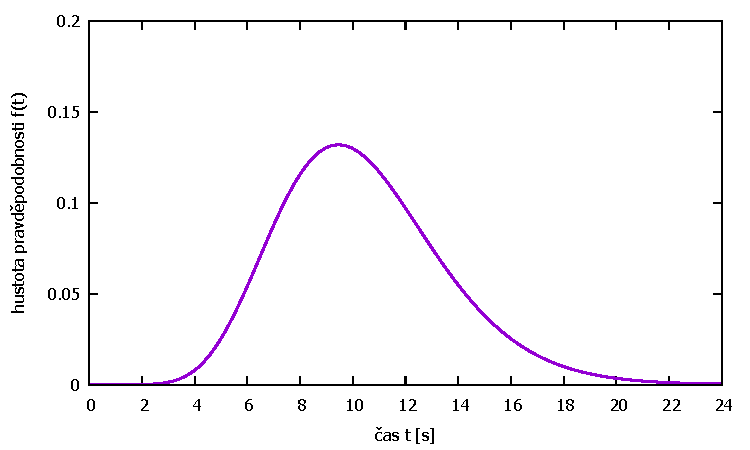
\includegraphics{obrazky-figures/gamma_distribution.pdf}
    \caption{Pravděpodobnostní rozdělení gama s~parametry $\alpha = 10{,}95$ a~$\beta = 0{,}95$. Toto rozdělení bylo použito pro výběr doby trvání mezi sebráním bonusu a~vygenerováním dalšího bonusu.}
    \label{fig:probability-bonus-countdown}
\end{figure}

\subsection*{Vygenerování nových bonusů}

V~této fázi se nejdříve zkontroluje, zda odpočet pro vygenerování nového bonusu uplynul. Pokud ano, vygeneruje se nový bonus s~pomocí třídy \texttt{StageBonuses}. Tato třída je popsána v~kapitole~\ref{sec:jadro-hry}.

Vizuálním výstupem této fáze je přidání nového bonusu na herní plochu.


\section{Entity řízené počítačem}
\label{sec:entity-rizene-pocitacem}

Vytvořit entity řízené počítačem bylo jedním z~hlavních cílů této práce. Entity využívají metody popsané v~kapitole~\ref{ch:umela-inteligence} pro rozhodování svých dalších kroků. Bylo vytvořeno několik typů entit, které se liší svým cílem a~způsobem, jakým se snaží svého cíle dosáhnout. Uživatel má možnost tyto entity začlenit do hry během nastavení hry. Toto bylo popsáno v~kapitole~\ref{sec:uzivatelske-rozhrani}.

\subsection{Prostředí hry}

V~kapitole~\ref{sec:reseni-uloh} byly popsány různé vlastnosti, podle kterých lze kategorizovat prostředí úlohy pro umělou inteligenci. V~této sekci bude prostředí hry \emph{Bubble Brawl} rozděleno podle těchto vlastností do příslušných kategorií.

\subsubsection*{Pozorovatelnost}

Prostředí hry \emph{Bubble Brawl} má velmi blízko \emph{plné pozorovatelnosti}, avšak zařazení hry do této kategorie brání bonusy. U~bonusů hráči nemohou zjistit, jaké množství života jim bude při sebrání doplněno. Také časovač pro generování bonusů běží na pozadí a~hráči tak nemohou zjistit, za jak dlouhou dobu bude vygenerován další bonus. Proto prostředí této hry spadá spíše do kategorie \emph{částečně pozorovatelných}.

Hovořilo se však o~tom, že u~\emph{plně pozorovatelných} prostředí má každý hráč přehled o~všech \emph{relevantních} aspektech stavu hry. Hráče nemusí při plánování akcí zajímat, jaké množství života mu bonus doplní. Co se týče generování bonusů, hráč nemusí vědět o~tom, že nějaký časovač existuje a~generování chápat jako čistě náhodnou událost. V~takovém případě nemusí hráč nahlížet na generování bonusů jako na \emph{nepozorovatelný} aspekt, ale na čistě \emph{stochastický}. Pokud tyto 2 zmíněné aspekty přestanou být pro hráče relevantní, pak může na prostředí hry nahlížet jako na \emph{plně pozorovatelné}.

\subsubsection*{Množství agentů}

Je jasné, že prostředí hry \emph{Bubble Brawl} je \emph{multiagentní}. Otázkou však je, zda je možné toto prostředí jednoznačně zařadit do kategorie \emph{konkurenčních} prostředí. Pravidla hry totiž \emph{neznemožňují} vytváření \emph{neformálních aliancí} \cite[s.\,166]{AI_Russel_Norvig}, díky kterým jeden agent vykonáním jedné akce může zvýšit \emph{míru výkonnosti} jak sobě, tak dalším agentům ze stejné aliance (například, 3 slabší hráči mohou cíleně zaútočit na jednoho silnějšího hráče). Pro tyto případy je nejlepší o~prostředí hry hovořit pouze jako o~\emph{multiagentním} a~dále nespecializovat.

\subsubsection*{Determinizmus}

Prostředí hry \emph{Bubble Brawl} je \emph{stochastické}; opět kvůli bonusům. Ačkoliv velká část následujícího stavu hry závisí na aktuálním stavu, generování bonusu i~určení množství života získaného z~bonusu jsou stochastické jevy. Nicméně, žádný z~aktuálně implementovaných agentů nebere na tyto jevy zřetel právě kvůli tomu, jak velkou část následujícího stavu lze odvodit ze stavu aktuálního.

\subsubsection*{Návaznost akcí}

Prostředí hry \emph{Bubble Brawl} jednoznačně patří do kategorie \emph{sekvenčních} prostředí. Přestože důsledky akcí nejsou tak dlouhodobé, jako například ve hře \emph{Šachy}, jednotlivé akce stále určitým způsobem ovlivňují budoucí rozhodování. Navíc, pokud agent nebude brát jako akci pouze stisk klávesy, ale přímo pohyb z~jednoho místa do jiného vzdálenějšího, důsledky budou daleko větší.

\subsubsection*{Proměnlivost}

Ačkoliv se na první pohled může zdát, že prostředí hry \emph{Bubble Brawl} je \emph{dynamické}, není tomu tak. Hra se nemůže posunout dále, dokud se každý hrající agent nerozhodne, jakou akci vykoná. Na druhou stranu, agenti jsou zpravidla implementováni tak, aby dobou svého rozhodování nezpomalovali průběh hry.

\subsubsection*{Diskrétní a spojité prostředí}

Stavový prostor hry je teoreticky spojitý\,--\,omezený pouze přesností reálných čísel v~procesoru. Někteří agenti si však tento prostor navzorkují \cite{MIT_OpenCourseWare:Incremental_Path_Planning} za účelem optimalizace hledání cesty v~tomto prostoru, a~prohledávají tedy \emph{diskrétní} stavový prostor. Jakým způsobem vzorkování probíhá je popsáno v~kapitole~\ref{sec:entity-rizene-pocitacem:tridy}.

Podle ostatních aspektů by prostředí mělo být \emph{diskrétní}. Čas se mění skokově (přibližně $60\times$ za sekundu) a~množina akcí, které agent může v~jednom okamžiku vykonat, je konečná.

\subsubsection*{Znalost}

Z~pohledu téměř všech agentů se dá říci, že prostředí hry \emph{Bubble Brawl} je \emph{známé}. Pouze \uv{slepí} agenti (\emph{Blind predator} a~\emph{Blind prey}) někdy nedokážou přesně odhadnout stav, do kterého se vykonáním určité akce přesunou.

\subsection{Třídy}
\label{sec:entity-rizene-pocitacem:tridy}

V~programu je obsaženo několik tříd, které zajišťují fungování umělé inteligence ve hře. Největší skupinou tříd jsou ty, které řídí chování entit\,--\,\emph{agenti} (pojem \emph{agent} byl popsán v~kapitole~\ref{sec:reseni-uloh}). Existují však také další třídy, které tito \emph{agenti} využívají pro své fungování.

Velmi důležité pro \emph{agenty} je rozhraní \texttt{GameStateAgentProxy}\footnote{Na rozdíl od většiny ostatních rozhraní v~programu nemá předponu \uv{\texttt{I}}. Důvodem je jednoduše přehlédnutí během návrhu, které se nakonec dostalo i~do implementace.}. Jeho účelem je umožnit \textbf{přístup k~aktuálnímu stavu hry}. Mimoto také obsahuje několik pomocných metod, jako například výpočet nové pozice hráče po vykonání akce. Konkrétní implementaci tohoto rozhraní poskytuje samotné jádro hry (třída \texttt{Core}). Rozhraní poskytuje následující metody:
\begin{itemize}
    \item \texttt{getPlayers()}\,--\,Tato metoda vrací informace o~všech hráčích ve hře. Je to asociativní pole (\texttt{std::unordered\_map}), kde klíče jsou unikátní identifikátory hráčů. Informace, které jsou o~hráčích poskytovány, jsou: pozice, množství života, rychlost, síla a~velikost.
    \item \texttt{getObstacles()}\,--\,Poskytuje přístup k~překážkám na herní ploše. Návratovou hodnotou \emph{není} seznam překážek, ale objekt typu \texttt{StageObstacles}, který přímo zprostředkovává interakci mezi hráči a~překážkami (viz kapitola~\ref{sec:jadro-hry}).
    \item \texttt{getStageGridModel()}\,--\,Poskytuje přístup k~\emph{mřížovému modelu} herní plochy, viz dále.
    \item \texttt{getPlayerMovementVector()}\,--\,Vypočítá vektor hráčova pohybu na základě jeho aktuální pozice, rychlosti a~požadované akce.
    \item \texttt{calculateNewPlayerPos()}\,--\,Určí novou pozici hráče na základě jeho pozice, rychlosti, požadované akce a~překážek na herní ploše.
\end{itemize}

Spousta agentů využívá třídu \texttt{StageGridModel}, která představuje \textbf{diskrétní model herní plochy} \cite{MIT_OpenCourseWare:Incremental_Path_Planning}. Při vytváření instance této třídy je konstruktoru předána množina všech překážek na herní ploše a~velikost herní plochy. Podle těchto informací je herní plocha navzorkována. Vzniká mřížka čtvercových buněk s~délkou strany 17~jednotek délky (tato délka odpovídá maximální délce posunu hráče během jednoho herního cyklu). Z~této mřížky jsou následně odstraněny buňky, které se překrývají s~překážkami.

U~každé buňky je možné zjistit souřadnice jejího středu, vzdálenost středu od nejbližší překážky a~nejvýše 8~buněk, se kterými daná buňka sousedí. Různí agenti si vybírají akci podle toho, jak blízko je dostane ke středu vybrané buňky. Vzdálenost buňky od nejbližší překážky využívají agenti, aby zjistili, zda dokážou projít danou buňkou.

Nejdůležitější pro implementaci \textbf{agentů} je rozhraní \texttt{IAIPlayerAgent}. Toto rozhraní obsahuje 4~metody:
\begin{itemize}
    \item \texttt{plan()}\,--\,Znamení agentovi, že může začít plánovat další akci.
    \item \texttt{assignProxy()}\,--\,Poskytne agentovi přístup k~aktuálnímu stavu hry (instanci rozhraní \texttt{GameStateAgentProxy}). Agent nemá možnost plánovat akce, dokud nemá možnost zjišťovat stav hry, a~proto musí být tato metoda zavolána před prvním voláním \texttt{plan()}.
    \item \texttt{kill()}\,--\,Ukončení činnosti agenta. Pokud agent funguje na principu \emph{vláken}, jsou všechna \emph{vlákna} ukončena.
    \item \texttt{getPlayerInput()}\,--\,Vrací agentem naplánovanou akci.
\end{itemize}

Rozhraní \texttt{IAIPlayerAgent} implementuje abstraktní třída \texttt{AIPlayerAgentBase}, ze které jsou odvozeny všechny další třídy implementující chování agentů. Tato třída byla navržena tak, aby plánování každého agenta využívalo paralelní zpracování pomocí \emph{vláken}. Nepovedlo se však implementovat funkční řešení tohoto návrhu, a~tedy veškeré plánování běží sériově.


\subsection{Jednotlivé typy entit}

Program obsahuje několik typů entit řízených počítačem, které se liší svým chováním. Cílem většiny entit je samozřejmě zvítězit, nicméně tento cíl je příliš abstraktní a~je nutné si jej rozdělit na menší dílčí cíle. Různé entity mají různé cíle, což se projevuje na jejich chování. Některé entity mohou mít stejné cíle, ale liší se v~postupu, jak jich dosáhnout.

Entity lze dle dílčích cílů rozdělit na 3 základní typy: \emph{predátoři}, kteří se snaží pouze útočit, \emph{kořisti}, které se snaží pouze utíkat, a~\emph{beruška}, která zdánlivě nemá cíl žádný. Entit stejných typů bylo implementováno více. Cílem bylo nahradit dříve implementované entity vylepšenými verzemi. Přesto však starší verze entit zůstaly v~aplikaci, aby lidé, kteří si hru zkusili zahrát, mohli posoudit, zda se vylepšení dané entity opravdu povedlo, nebo zda původní verze dokázala hrát hru lépe.

\emph{Predátoři} a~\emph{kořisti} jsou entity založené na ohodnocování hráčů. V~každém herním cyklu ohodnotí všechny soupeře podle jejich síly a~vzdálenosti mezi sebou a~daným soupeřem a~na základě získaných ohodnocení činí rozhodnutí. Všechny varianty \emph{predátorů} mají stejný postup ohodnocování soupeřů, a~sice:

\begin{eqnarray}
    \label{eq:opponent-health-predator}
    f_h(p) & = & 10 \cdot \frac{1}{h(p)} \\
    \label{eq:opponent-distance-predator}
    f_d(p) & = & 30 \cdot \frac{1}{d^2(p)} \\
    \label{eq:opponent-eval-predator}
    f(p) & = & f_h(p) + f_d(p)
\end{eqnarray}
Rovnice~\eqref{eq:opponent-health-predator} ukazuje výpočet ohodnocení hráče~$p$ podle množství jeho života, v~níž funkce $h(p)$ představuje aktuální množství života hráče~$p$. Rovnice~\eqref{eq:opponent-distance-predator} ukazuje výpočet ohodnocení hráče $p$ podle vzdálenosti od hodnotící entity, kde funkce $d^2(p)$ představuje druhou mocninu této vzdálenosti. Nakonec, rovnice~\eqref{eq:opponent-eval-predator} ukazuje výpočet celkového ohodnocení hráče~$p$. Jak množství života, tak vzdálenost jsou nepřímo úměrné příslušnému ohodnocení. To znamená, že čím nižší je množství života a~vzdálenost daného soupeře, tím lepší je jeho ohodnocení. Obě ohodnocení jsou navíc násobena konstantou větší než~1 za účelem ovlivnění jejich významnost ve výsledku. Tyto konstanty byly vybrány zcela nahodile. Důvodem použití druhé mocniny vzdálenosti je především vyvarování se výpočetně náročné operaci odmocňování (inspirace v~\cite{CGAL_Exact_Computation_paradigm}).

Podobný postup ohodnocování soupeřů mají všechny \emph{kořisti}:
\begin{eqnarray}
    \label{eq:opponent-health-prey}
    f_h(p) & = & -10 \cdot h(p) \\
    \label{eq:opponent-distance-prey}
    f_d(p) & = & -30 \cdot \frac{1}{d^2(p)} \\
    \label{eq:opponent-eval-prey}
    f(p) & = & f_h(p) + f_d(p)
\end{eqnarray}
Význam jednotlivých proměnných a~funkcí zůstává stejný, jako v~rovnicích výše. Soupeřovo množství života je tentokrát přímo úměrné a~vzdálenost nepřímo úměrná příslušnému ohodnocení. Jelikož jsou tentokrát obě ohodnocení násobena zápornou konstantou, jejich význam je opačný: čím vyšší množství života má soupeř, tím nižší je jeho ohodnocení (tím je nebezpečnější), a~čím vyšší je vzdálenost od něj, tím vyšší je jeho ohodnocení (tím je méně nebezpečný).

Následuje seznam entit a~popis jejich fungování. Jejich jména zde odpovídají jménům, jak jsou zobrazena v~aplikaci. Pouze entity \emph{Wall-aware BFS predator}, \emph{IDS predator} a~\emph{BFS predator} jsou vynechány ze seznamu entit v~aplikaci, protože jejich výkonnost byla příliš nízká. Tyto entity lze opět zařadit do seznamu zakomentováním příslušného řádku\footnote{Jde o~řádek \texttt{add\_compile\_definitions(EXCLUDE\_SLOW\_AGENTS)}.} v~souboru \texttt{CMakeLists.txt} a~opětovným sestavením aplikace.

\subsubsection*{Ladybug}

\emph{Ladybug} (\emph{beruška}) je jednou z~prvních implementovaných entit. Jejím jediným cílem je pohybovat se přirozeně. Entita se snaží neměnit směr příliš rychle a~občas se zastavit, což může připomínat pohyb hmyzu (odtud název). Implementace chování této entity je následující:
\begin{enumerate}
    \item S~pravděpodobností~$15/16$ vykonej stejnou akci, jakou jsi vykonala naposledy. Jinak pokračuj.
    \item Pro každý ze 4 směrů (nahoru, dolů, doleva, doprava) nastav stav \uv{stisknuto} s~pravděpodobností~$1/2$, jinak na \uv{nestisknuto} a~výslednou akci vykonej.
\end{enumerate}
Na začátku platí stav \uv{nestisknuto} pro všechny 4 směry, tedy žádný pohyb.

\subsubsection*{Blind predator a Blind prey}

Entity \emph{Blind predator} a~\emph{Blind prey} patří mezi entity, které plánují pouze jeden krok dopředu. V~každém kroku se snaží vykonat akci, díky které dosáhnou stavu s~nejlepším ohodnocením. Ohodnocení stavu je dáno součtem ohodnocení všech soupeřů pro daný stav. Implementace chování obou entit je velmi podobná; liší se pouze ve způsobu ohodnocování soupeřů:
\begin{enumerate}
    \item Pro každou z~9~akcí (pohyb jedním z~8~směrů nebo žádný pohyb) spočítej ohodnocení následníka aktuálního stavu dosažitelného vykonáním dané akce.
    \item Vykonej akci, která vede do stavu s~nejlepším ohodnocením.
\end{enumerate}

Přívlastek \emph{blind} (\emph{slepý}) souvisí s~tím, že při rozhodování neberou v~potaz překážky na herní ploše (\uv{nevidí je}). Vykonání akce pro ně tedy znamená posunout se požadovaným směrem o~vzdálenost \emph{přesně} danou množstvím jejich života. Důsledkem toho je, že pokud tyto entity narazí na překážku, budou se domnívat, že tam žádná překážka není a~zůstanou stát na místě.

\subsubsection*{Wall-aware predator a Wall-aware prey}

Entity \emph{Wall-aware predator} a~\emph{Wall-aware prey} jsou opět entity, které dokážou plánovat pouze jeden krok dopředu. Implementace jejich chování je téměř stejná, jako implementace jejich \emph{blind} protějšků. Rozdílem však je, že tyto entity dokážou vnímat překážky na herní ploše, a~jsou tedy lépe informované o~tom, jaký důsledek bude mít která jejich akce.

Zlepšení chování je pozorovatelné především u \emph{kořisti} (\emph{Wall-aware prey}). Pokud je pronásledována soupeřem podél zdi a~dostane se do rohu, dokáže v~některých případech změnit směr a~pohybovat se podél zdi kolmé k~původní zdi. Přesto, ve spoustě případů entita v~rohu uvízne. Ani \emph{predátorovi} (\emph{Wall-aware predator}) toto zlepšení příliš nepomůže; pokud pronásleduje svou oběť a~v~cestě mu stojí jen velmi malá překážka, většinou nezvládne najít cestu okolo ní.

\subsubsection*{Wall-aware BFS predator}

Tato entita kombinuje metodu \emph{slepého prohledávání do šířky} (\emph{BFS}) a~implementaci generování akcí stejnou jako \emph{Wall-aware predator}. Jejím cílem při výběru dalšího kroku není najít nejoptimálnější stav, ale vybrat sousední stav, který leží na cestě vedoucí k~jednomu konkrétnímu soupeři. Entita si v~každém kroku vybírá nejlepší oběť a~počítá celou cestu vedoucí k~této oběti. Popis implementace chování entity je následující:
\begin{enumerate}
    \item Spočítej ohodnocení všech svých soupeřů pro aktuální stav a~vyber soupeře s~nejlepším ohodnocením jako svoji \emph{oběť}.
    \item Pokud se s~\emph{obětí} už dotýkáš, nevykonávej žádnou akci. Jinak pokračuj.
    \item Pomocí metody \emph{BFS s~kolekcí CLOSED} najdi cestu vedoucí z~tvojí aktuální pozice k~vybrané \emph{oběti}. Cílovou podmínkou budiž situace, kdy se při vykonání akce dotkneš svojí \emph{oběti}.
    \item Pokud nebyl nalezen cílový uzel, nevykonávej žádnou akci. Jinak pokračuj.
    \item Z~cílového uzlu najdi cestu vyhledávacím stromem zpět k~uzlu, který je bezprostředním následníkem kořene. Vykonej akci vedoucí z~kořenového uzlu do tohoto následníka.
\end{enumerate}

Entita má poměrně dobré znalosti o~důsledcích svých akcí. Na rozdíl od entit plánujících pouze jeden krok dopředu zná celou cestu až ke svojí oběti a~na rozdíl od entit využívající diskrétní model herní plochy dokáže projít i~úzkými průchody, které tyto entity mohou vyhodnotit jako neprůchozí. Velkou nevýhodou této entity je však dlouhá doba plánování. I~při velmi krátkých vzdálenostech od svého cíle trvá plánování entity nepřijatelně dlouhou dobu, jak je ukázáno v~kapitole~\ref{sec:vykonnostni-testovani}.

\subsubsection*{IDS predator}

Tato entita využívá diskrétní model herní plochy, na němž hledá cestu ke svojí \emph{oběti} pomocí metody \emph{postupného zanořování do hloubky} (\emph{IDS}). V~implementaci však není použito klasické \emph{IDS}; zatímco běžná implementace této metody opakovaně volá metodu \emph{slepého prohledávání do hloubky} (\emph{DFS}) s~omezenou hloubkou stromu, v~implementaci chování této entity je místo toho opakovaně volána metoda \emph{zpětného navracení} (\emph{Backtracking}). Záměrem bylo více optimalizovat paměťovou náročnost algoritmu. Popis implementace chování entity je následující:
\begin{enumerate}
    \item Spočítej ohodnocení všech svých soupeřů pro aktuální stav a~vyber soupeře s~nejlepším ohodnocením jako svoji \emph{oběť}.
    \item Pokud se \emph{oběť} nachází ve stejné buňce jako ty, nevykonávej žádnou akci. Jinak pokračuj.
    \item Pomocí modifikované metody \emph{IDS} najdi cestu vedoucí z~buňky, v~níž se nacházíš, do buňky, v~níž se nachází tvoje \emph{oběť}.
    \item Pokud nebyl nalezen cílový uzel, nevykonávej žádnou akci. Jinak pokračuj.
    \item Vykonej akci podle toho, v~jakém směru od kořenového uzlu se nachází jeho bezprostřední následník.
\end{enumerate}

V~každém uzlu může agent vykonat pouze 4~akce (svislý a~vodorovný pohyb) místo obvyklých 8. Původní myšlenka byla taková, že při diagonálních akcích nelze s~jistotou říci, zda průchod mezi diagonálně sousedícími buňkami je dostatečně široký. Tento problém se však týká i~svisle a~vodorovně sousedících buněk. Nakonec však toto omezení zůstalo z~důvodu snížení faktoru větvení vyhledávacího stromu, a~tedy urychlení plánování agentů.

Doba plánování entity je sice kratší, nicméně stále není dostatečně krátká, aby se dala považovat za přijatelnou. Testy však ukázaly, že prostorová náročnost při plánování je zanedbatelná oproti náročnosti časové (viz kapitola~\ref{sec:vykonnostni-testovani}). Proto se ostatní entity zaměřují na optimalizaci doby plánování na úkor využitého množství paměti.

\subsubsection*{BFS predator}

Implementace chování entity \emph{BFS predator} je ve většině ohledů stejná, jako implementace chování entity \emph{IDS predator}. Jediný rozdíl je použití metody \emph{slepého prohledávání do šířky s~kolekcí CLOSED} (\emph{BFS s~kolekcí CLOSED}) místo metody \emph{IDS}.

Díky velkému snížení počtu generování uzlů se mnohonásobně zkrátila doba plánování, jak je ukázáno v~kapitole~\ref{sec:vykonnostni-testovani}. Tato optimalizace téměř stačí na to, aby byla entita považována za začlenitelnou do hry. Problémem však stále zůstává, že entita není \emph{stabilní}. Doba plánování entity není omezena, a~proto na větších herních plochách může stále zpomalovat běh programu.

\subsubsection*{A* predator}

Entita \emph{A* predator} se stále implementačně podobá entitám \emph{IDS predator} a~\emph{BFS predator}. Základní algoritmus je téměř stejný, pouze s~obměnou metody \emph{IDS}/\emph{BFS} za metodu \emph{A*}. Nastalo však několik dalších změn.

Tato entita hledá cestu ke svojí oběti, ale přestane hledat, jakmile vygeneruje 5\,000.~uzel. Tato změna zaručuje, že plánování agenta bude \emph{stabilní}, tady ani na příliš velkých herních plochách by neměla zpomalovat běh programu. Číslo 5\,000 bylo vybráno na základě testování tak, aby při hře 8~hráčů tohoto typu běžela aplikace dostatečně rychle i~na méně výkonných počítačích. Po vygenerování tohoto množství uzlů však není prohledávání rovnou ukončeno jako neúspěšné. Jak se má postupovat dále je určeno verzí entity.

Entita \emph{A* predator} byla několikrát vylepšena, ale předchozí implementace v~kódu zůstaly. Jejich aktivace je možná nastavením hodnoty makra \texttt{ASTAR\_PREDATOR\_VERSION} v~souboru \texttt{AstarPredatorAIPlayerAgent.hpp}. Verze 1~entity po dosažení maximálního počtu vygenerovaných uzlů zvolí uzel na vrcholu kolekce \emph{OPEN} jako cílový uzel. To samé činí i~verze~2 této entity. Vylepšení v~této verzi naopak spočívá ve výběru akce po dokončení hledání cesty. Entita \uv{vyzkouší} vykonat všech 8~možných pohybů a~vybere si ten, který ji dostane nejblíže k~bezprostřednímu následníku kořenového uzlu. Poslední, 3. verze entity opět mění způsob výběru cílového uzlu po vygenerování maximálního počtu uzlů. Vybrán je ten, jehož ohodnocení heuristikou $h(s_k)$ je ze všech uzlů v~kolekci \emph{CLOSED} nejnižší (jinými slovy, jehož vzdálenost od cílového uzlu je nejnižší).

Entita je velmi schopná v~plnění svého cíle, tedy v~pronásledování svojí oběti. I~přes omezení počtu vygenerovaných uzlů má velkou šanci zvolit správnou cestu v~případě, že po dosažení tohoto limitu nedorazí do cílového uzlu. Také doba plánování této entity je velmi uspokojivá. Ovšem nevýhodou je velmi malá šance na přežití. Jelikož se entita snaží pouze útočit a~nevyhledává bonusy, je jednoduché ji velice brzy vyřadit ze hry.

\subsubsection*{Minimax prey}

Entita \emph{Minimax prey} se snaží hledat optimální stav pomocí metody \emph{Minimax}. Vybírá si soupeře, který ji nejvíce ohrožuje, jako útočníka. Následně se snaží předpovědět jeho chování, a~podle toho pak hledat optimální stav. Entita opět používá diskrétní model herní plochy pro plánování. Popis implementace chování entity je následující:
\begin{enumerate}
    \item Spočítej ohodnocení všech svých soupeřů pro aktuální stav a~vyber soupeře s~nejhorším ohodnocením jako svého \emph{útočníka}.
    \item Pomocí metody \emph{Minimax} najdi optimální stav. Hráč \emph{Max} jsi ty, hráč \emph{Min} je tvůj \emph{útočník}.
    \item Urči bezprostředního následníka kořenového uzlu, který leží na cestě k~nalezenému optimálnímu stavu. Vykonej pohyb, který tě k~tomuto následníku dostane nejblíže.
\end{enumerate}

Opět bylo vyvinuto několik verzí této entity\,--\,konkrétně 2. Nastavit jinou lze změnou hodnoty makra \texttt{MINIMAX\_PREY\_VERSION} v~souboru \texttt{MinimaxPreyAIPlayerAgent.hpp}. Tyto verze se liší pouze v~použité metodě hledání cesty. První verze používá obyčejnou metodu \emph{Minimax}, verze~2 pak metodu \emph{Alfa-beta řezů}.

Ačkoliv je metoda \emph{Minimax} určena především pro hry, kde se hráči na tahu střídají, povedlo se ji implementovat i~pro tuto hru. Aby však plánování netrvalo příliš dlouho musela být maximální hloubka vyhledávacího stromu stanovena na velmi malé číslo. Verze~1, která používá obyčejnou metodu \emph{Minimax}, má nastavenou maximální hloubku 6, druhá verze, která využívá \emph{Alfa-beta řezy}, má nastavenou maximální hloubku 8. Jak je ukázáno v~kapitole~\ref{sec:vykonnostni-testovani}, větší hodnoty hloubky by mohly zpomalovat běh programu. Kvůli nízké hloubce vyhledávacího stromu nemá tato entita o~mnoho lepší schopnosti, než \uv{slepá} entita \emph{Wall-aware prey}.

\subsection{Nevyužité metody řešení úloh}

V~kapitole~\ref{ch:umela-inteligence} bylo představeno několik metod řešení úloh a~hraní her. Spousta z~nich byla použita pro implementaci chování entit řízených počítačem, ale některé se do implementace nedostaly. Tato sekce se věnuje důvodům, proč nebyly tyto metody v~implementaci použity.

Z~neinformovaných metod prohledávání stavového prostoru byly v~práci použity pouze 2: \emph{slepé prohledávání do šířky} (\emph{BFS}) a~\emph{postupné zanořování do hloubky} (\emph{IDS}). Ostatní jsou v~práci použity nepřímo, například \emph{zpětné navracení} (\emph{Backtracking}) a~\emph{omezené prohledávání do hloubky} (\emph{DLS}) jako součást metody \emph{IDS}, nebo \emph{slepé prohledávání do hloubky} (\emph{DFS}) jako součást metody \emph{Minimax}. Jediná neinformovaná metoda, kterou se nepodařilo využít ani nepřímo, je metoda \emph{stejných cen} (\emph{UCS}). Žádná z~entit nepoužívá při hledání cesty ohodnocení přechodů mezi stavy, a~tudíž by se tato metoda neuplatnila.

Z~informovaných metod byla využita pouze jedna, a~to metoda \emph{A*}. Ostatní informované metody pouze zvyšují výkonnost metody \emph{A*}. Jelikož entita využívající tuto metodu (entita \emph{A* predator}) plánuje velmi rychle, nebylo nutné ji dále vylepšovat. Mimoto u~některých metod se později ukázalo, že nejsou příliš vhodné pro tento typ úlohy. Aby se projevila účinnost metody \emph{Lifelong Planning A*}, musely by entity brát v~úvahu přechody mezi stavy. To stejné platí i~pro metodu \emph{D* Lite}. Navíc tato metoda vyžaduje, aby v~každém jejím volání (tedy v~každém herním cyklu) zůstal cílový uzel stejný. Jelikož cílem jsou většinou ostatní hráči, kteří se po herní ploše pohybují, tato metoda by v~tomto případě použitelná vůbec nebyla. Metoda \emph{Anytime Repairing A*} vyžaduje, aby napříč jejími voláními (napříč herními cykly) zůstal stav úlohy stejný, což v~multiagentních prostředích zaručit nelze.

Metody hraní her byly v~aplikaci použity 2: \emph{Minimax} a~\emph{Alfa-beta řezy}. Metody \emph{Max\textsuperscript{n}} a~\emph{Shallow pruning} nebylo možné využít především z~výkonnostních důvodů. Samy \emph{Minimax} i~\emph{Alfa-beta řezy} byly pro tuto hru příliš výkonnostně náročné. Metody \emph{Max\textsuperscript{n}} a~\emph{Shallow pruning} generují oproti nim mnohem větší počet uzlů, a~mají tedy větší časové nároky. Z~toho bylo možné usoudit, že tyto metody v~implementaci chování entit neobstojí.


\chapter{Testování}
\label{ch:testovani}

Tato kapitola se zabývá zhodnocením funkčnosti výsledného programu. Pro zhodnocení byly použity dva přístupy. První část této kapitoly se věnuje testování výkonnosti programu. Zaměřuje se především na výkonnostní testování jádra hry a~entit řízených počítačem. Druhá část této kapitoly se pak věnuje zpětné vazbě od uživatelů, kteří si vyzkoušeli používání aplikace.

\section{Výkonnostní testování}
\label{sec:vykonnostni-testovani}

V~této sekci jsou ukázány výsledky měření výkonnosti různých částí aplikace. Cílem měření bylo především zjistit, jak implementovat entity řízené počítačem, aby nezpomalovaly chod aplikace. Měřen byl čas strávený při vykonávání různých funkcí v~programu. Pokud není řečeno jinak, pak testy byly provedeny v~prostředí s~těmito vlastnostmi:
\begin{itemize}
    \item operační systém: Windows 11 Pro, verze 23H2,
    \item procesor: AMD Ryzen 7 5700U with Radeon Graphics, 1.80 GHz,
    \item RAM: 16 GB.
\end{itemize}
Na pozadí běžely další procesy, jako například antivirus, internetový prohlížeč aj., aby zátěž byla přibližně taková, jaká by mohla být při běžném používání aplikace. Pro měření byla použita třída \texttt{Benchmark} ze souboru \texttt{utility/benchmark/Benchmark.hpp}. Ve výsledné aplikaci je tato třída vyřazena ze sestavování; pro její začlenění do aplikace lze nastavit v~souboru \texttt{CMakeLists.txt} proměnnou \texttt{INCLUDE\_BENCHMARK} na hodnotu \texttt{TRUE} (příkaz \texttt{set(INCLUDE\_BENCHMARK TRUE)}). Stojí za připomenutí, že doba mezi herními cykly je 17\,ms. V~ideálním případě by tedy vše, co souvisí s~herním cyklem, mělo být vykonáno během této doby.

\subsection*{Hra bez umělých hráčů}

Tabulka~\ref{tab:benchmark-basics} ukazuje průměrnou dobu trvání vykonání všech kroků herního cyklu (řádek \uv{Změna stavu hry}) a~vizuální výstup těchto změn (řádek \uv{Výstup na obrazovku}). Ve hře bylo vždy 8 hráčů a~každá průměrná hodnota byla vypočítána z~přibližně 300 záznamů měření (přibližně 5,1\,s běhu programu). Pro testování byly použity tyto 2 herní plochy: \emph{Too many players} a~\emph{Shattered glass}. Důvodem výběru těchto 2 herních ploch je počet překážek\,--\,zatímco \emph{Too many players} nemá překážku žádnou, \emph{Shattered glass} jich má 51. Díky tomuto lze dobře porovnat vliv množství překážek na výkon aplikace. Tabulka se na tyto herní plochy neodkazuje jejich jménem, ale přímo počtem překážek.

\begin{table}[ht]
    \centering
    \begin{tabular}{|l|c|c|} \hline
        \textbf{Počet překážek}      & \textbf{0} & \textbf{51} \\ \hline\hline
        \textbf{Změna stavu hry}     & 0,031      & 0,057       \\ \hline
        \textbf{Výstup na obrazovku} & 3,581      & 5,327       \\ \hline
    \end{tabular}
    \caption{Průměrná doba trvání základních operací souvisejících s~herním cyklem (v~milisekundách).}
    \label{tab:benchmark-basics}
\end{table}

Z~testu lze vypozorovat, že herní cyklus samotný není příliš výkonnostně náročný, a~to ani při rostoucím množství překážek. Naopak, zobrazení stavu hry na obrazovce zabere poměrně výraznou část doby mezi herními cykly\,--\,více než 20\,\%. S~přidáním většího množství překážek také poměrně výrazně vzrostla doba zpracování\,--\,přibližně o~10\,\% doby mezi herními cykly.

Pokud entita řízená počítačem má být použita v~aplikaci, pak doba, kterou stráví plánováním, by měla být menší než $11{,}673\text{\,ms} = 17\text{\,ms} - 5{,}327\text{\,ms}$. Tuto dobu může entita strávit plánováním, pokud bude ve hře pouze 1. Maximální počet hráčů ve hře je však 8, a~proto, pokud by mělo být zapojeno 8~entit daného typu, měla by být doba plánování maximálně $1{,}46\text{\,ms} = 11{,}673\text{\,ms} : 8$. Tyto časy jsou shrnuty v~tabulce~\ref{tab:times-summary}.

\begin{table}[ht]
    \centering
    \begin{tabular}{|p{0.4\textwidth}|c|} \hline
         & \textbf{Čas [ms]} \\ \hline
        \textbf{Doba mezi herními cykly}                    & 17    \\ \hline
        \textbf{Přibližná doba trvání výstupu na obrazovku} & 5,327 \\ \hline
        \textbf{Maximální doba plánování 1~agenta (při hře 1~agenta)} & 11,673 \\ \hline
        \textbf{Maximální doba plánování 1~agenta (při hře 8~agentů)} & 1,46   \\ \hline
    \end{tabular}
    \caption{Shrnutí časů potřebných pro vykonání různých akcí.}
    \label{tab:times-summary}
\end{table}

\subsection*{Jednoduší agenti}

Tabulka~\ref{tab:benchmark-simple-bots} ukazuje průměrnou dobu plánování agentů typu \emph{Ladybug}, \emph{Blind predator} a~\emph{Blind prey}. Tito agenti nevyužívají při plánování ani překážky na herní ploše, ani diskrétní model herní plochy. Je tedy zřejmé, že doba plánování nebude ovlivněna počtem překážek, nicméně kvůli konzistentnosti jsou data v~tabulce opět rozdělena do 2 sloupců podle tohoto kritéria. Asi není žádným překvapením, že doba plánování těchto agentů je velmi krátká. \emph{Ladybug} používá pouze generátor náhodných čísel a~bitové operace. \emph{Blind predator} a~\emph{Blind prey} sice používají náročnější aritmetické operace a~doba jejich plánování je tím pádem zhruba 4\texttimes{} delší, ale i~přesto lze říct, že tato doba je naprosto zanedbatelná.

Pro testování byly použity herní plochy \emph{Too many players} a~\emph{Shattered glass} ze stejného důvodu, jako v~případě předcházejícího testu.

\begin{table}[ht]
    \centering
    \begin{tabular}{|l|c|c|} \hline
        \textbf{Počet překážek} & \textbf{0}  & \textbf{51} \\ \hline\hline
        \textbf{Ladybug}        & 0,000\,29   & 0,000\,29   \\ \hline
        \textbf{Blind predator} & 0,000\,98   & 0,001\,3    \\ \hline
        \textbf{Blind prey}     & 0,001       & 0,001       \\ \hline
    \end{tabular}
    \caption{Průměrná doba plánování jednoduchých agentů (v~milisekundách).}
    \label{tab:benchmark-simple-bots}
\end{table}

\subsection*{Wall-aware agenti}

Tabulka~\ref{tab:benchmark-wall-aware-bots} ukazuje průměrnou dobu plánování agentů typu \emph{Wall-aware predator} a~\emph{Wall-aware prey}. Tito agenti při plánování berou v~potaz překážky na herní ploše, ale plánují pouze jeden krok dopředu. Začlenění překážek do procesu rozhodování způsobuje, že činnost agenta trvá 2--3\texttimes{} delší dobu na herní ploše bez překážek a~více než 20\texttimes{} delší dobu s~51 překážkami. I~přesto zabere plánování těchto agentů přibližně 0,1\,\% z~celkové doby mezi herními cykly, tedy velmi zanedbatelné množství času. Z~tohoto důvodu fungují na podobném principu některé části implementace chování i~jiných typů agentů.

Pro testování byly použity tyto herní plochy \emph{Too many players} a~\emph{Shattered glass} ze stejného důvodu, jako v~případě předcházejících dvou testů.

\begin{table}[ht]
    \centering
    \begin{tabular}{|l|c|c|} \hline
        \textbf{Počet překážek}      & \textbf{0}  & \textbf{51} \\ \hline\hline
        \textbf{Wall-aware predator} & 0,002\,55   & 0,024\,23   \\ \hline
        \textbf{Wall-aware prey}     & 0,003\,69   & 0,027\,4    \\ \hline
    \end{tabular}
    \caption{Průměrná doba plánování \uv{wall-aware} agentů (v~milisekundách).}
    \label{tab:benchmark-wall-aware-bots}
\end{table}

\subsection*{Wall-aware BFS predator}

Tabulka~\ref{tab:benchmark-wall-aware-bfs-predator} obsahuje část výsledků měření výkonnosti agenta \emph{Wall-aware BFS predator}. Chování tohoto agenta je mírně odlišné od dosud testovaných agentů\,--\,zatímco předchozí agenti plánovali pouze jeden krok dopředu, \emph{Wall-aware BFS predator} plánuje celou cestu až ke své oběti. Proto nemělo cenu měřit průměrnou dobu plánování, jelikož každý proces plánování může trvat různě dlouhou dobu. Tabulka obsahuje 3 sloupce: hodnoty v~prvním sloupci představují vzdálenost mezi \emph{kružnicemi} hráčů, v~druhém sloupci počet vygenerovaných uzlů metodou \emph{BFS} a~ve třetím čas v~milisekundách strávený plánováním. Testování probíhalo pouze na herní ploše \emph{Too many players}; na ploše \emph{Shattered glass} nedokázal agent učinit rozhodnutí ani po 10~minutách plánování, a~testování tím pádem nedávalo příliš smysl (celkově, agent, který nedokáže učinit rozhodnutí ani do oněch 17\,ms času mezi herními cykly, je prakticky nepoužitelný).

\begin{table}[ht]
    \centering
    \begin{tabular}{|c|c|c|} \hline
        \textbf{Vzdálenost} & \textbf{Počet uzlů} & \textbf{Čas [ms]} \\ \hline
        84,39               & 9\,625\,778         & 11\,550,2    \\ \hline
        47,69               & 1\,225\,619         & 934,489      \\ \hline
        22,33               & 24\,110             & 11,396       \\ \hline
        11,09               & 1\,078              & 0.593        \\ \hline
    \end{tabular}
    \caption{Doba a~počet uzlů vygenerovaných během plánování agenta \emph{Wall-aware BFS predator} v~závislosti na vzdálenosti mezi jeho \emph{kružnicí} a~\emph{kružnicí} jeho oběti.}
    \label{tab:benchmark-wall-aware-bfs-predator}
\end{table}

Záznamy měření v~tabulce byly vybrány systematicky podle délky trvání. První záznam je nejdelší zaznamenaná doba plánování agenta během hry. Druhý záznam je první plánování, jehož doba je kratší než 1~sekunda. Třetí a~čtvrtý záznam jsou první plánování, které splňují maximální doby plánování 1~agenta podle tabulky~\ref{tab:times-summary}.

Už podle prvního záznamu lze usoudit, že tento agent není prakticky použitelný pro běžné hraní. Hráči od sebe mohou být na herní ploše vzdálení až 1000 jednotek vzdálenosti a~tento agent již při pouhých 84 jednotkách plánuje celých 11,5~sekundy.

Za povšimnutí stojí také rozdíl vzdálenosti a~počtu uzlů mezi prvním a~druhým záznamem. Zatímco vzdálenost je přibližně 2\texttimes{} nižší, počet uzlů klesl téměř o 9násobek. Zde se projevuje časová složitost metody \emph{BFS}\,--\,se zvyšující se hloubkou vyhledávacího stromu, v~níž se nachází cílový uzel, roste počet generovaných uzlů exponenciálně.

Tento test ukázal, že není výhodné provádět plánování opakovaným zkoušením vstupů z~klávesnice. Proto další agenti začali používat diskrétní model herní plochy, který pracuje efektivněji.

\subsection*{IDS predator}

Tabulka~\ref{tab:benchmark-ids-predator} obsahuje část výsledků měření výkonnosti agenta \emph{IDS predator}. Tento agent využívá při plánování diskrétní model herní plochy a~plánuje celou cestu až ke své oběti. Sloupce tabulky ukazují vzdálenost mezi pozicemi agenta a~jeho oběti, počet uzlů vygenerovaných metodou \emph{IDS} a~čas strávený plánováním. Záznamy měření byly vybírány stejným způsobem, jako v~případě agenta \emph{Wall-aware BFS predator}. Zde je však tabulka rozdělena na 2~části. V~první části byla použita herní plocha  \emph{Too many players}, v~druhé pak plocha \emph{Shattered glass}.

\begin{table}[ht]
    \centering
    \begin{tabular}{|c|c|c|} \hline
        \textbf{Vzdálenost} & \textbf{Počet uzlů} & \textbf{Čas [ms]} \\ \hline\hline
        \multicolumn{3}{|c|}{\textbf{Počet překážek: 0}}              \\ \hline
        184,39              & 38\,862\,057        & 3\,873,61         \\ \hline
        165,86              & 5\,346\,717         & 537,386           \\ \hline
        128,69              & 99\,989             & 10,359            \\ \hline
        117,83              & 5\,714              & 0,921             \\ \hline\hline
        \multicolumn{3}{|c|}{\textbf{Počet překážek: 51}}             \\ \hline
        266,83              & 108\,316\,298       & 10\,787           \\ \hline
        220,17              & 6\,647\,559         & 655,84            \\ \hline
        153,75              & 91\,528             & 9,446             \\ \hline
        116                 & 12\,352             & 1,197             \\ \hline
    \end{tabular}
    \caption{Doba a~počet uzlů vygenerovaných během plánování agenta \emph{IDS predator} v~závislosti na vzdálenosti od jeho oběti.}
    \label{tab:benchmark-ids-predator}
\end{table}

Je patrné, že tento agent plánuje mnohem rychleji, než \emph{Wall-aware BFS predator}. Přestože počet generovaných uzlů roste rychleji se zvyšující se vzdáleností od oběti, čas využitý při jejich generování a~prozkoumávání je mnohem nižší. Stále je však doba plánování příliš dlouhá i~pro malé vzdálenosti.

Dále je také vidět, že díky použití diskrétního modelu není doba výpočtu ovlivněna počtem překážek na herní ploše. Vzdálenosti všech buněk od překážek byly vypočítány před začátkem hry, a~agent nyní pouze porovnává svůj poloměr s~konkrétními hodnotami.

Test ukázal, že použití diskrétního modelu při plánování je velmi výhodné z~hlediska rychlosti plánování. Zároveň ukázal, že při použití tohoto modelu jsou požadavky na paměť daleko menší oproti požadavkům na dobu plánování\,--\,za přijatelnou dobu je možné vygenerovat přibližně 16\,000 uzlů. Proto nedává smysl používat metody, které jsou navrženy tak, aby šetřily paměť (a~mezi něž patří i~metoda \emph{IDS}).

\subsection*{BFS predator}

Agent \emph{BFS predator} využívá při plánování diskrétní model herní plochy a~plánuje celou cestu až ke své oběti pomocí metody \emph{BFS s~kolekcí CLOSED}. Tabulka~\ref{tab:benchmark-bfs-predator-compare-ids} ukazuje část výsledků měření jeho výkonnosti, jejíž sloupce obsahují vzdálenost od vybrané oběti, počet uzlů vygenerovaných metodou \emph{BFS} a~čas strávený plánováním v~tomto pořadí. Test probíhal pouze na herní ploše \emph{Too many players}. Tabulka~\ref{tab:benchmark-bfs-predator-limits} také ukazuje část výsledků měření výkonnosti tohoto agenta, ale první sloupec tentokrát obsahuje rozměry herní plochy, na níž probíhalo testování. Tento test probíhal na herní ploše \emph{Enormous stage} s~upravenými rozměry.

\begin{table}[ht]
    \centering
    \begin{tabular}{|c|c|c|} \hline
        \textbf{Vzdálenost} & \textbf{Počet uzlů} & \textbf{Čas [ms]} \\ \hline
        184,39              & 1\,688              & 0,473             \\ \hline
        165,86              & 1\,320              & 0,293             \\ \hline
        128,69              & 680                 & 0,158             \\ \hline
        117,83              & 316                 & 0,086             \\ \hline
    \end{tabular}
    \caption{Doba a~počet uzlů vygenerovaných během plánování agenta \emph{BFS predator} v~závislosti na vzdálenosti od jeho oběti.}
    \label{tab:benchmark-bfs-predator-compare-ids}
\end{table}

\begin{table}[ht]
    \centering
    \begin{tabular}{|c|c|c|} \hline
        \textbf{Rozměry HP}       & \textbf{Počet uzlů} & \textbf{Čas [ms]} \\ \hline
        11\,800\texttimes{}6\,000 & 954\,945            & 988,216           \\ \hline
        2\,800\texttimes{}1\,700  & 59\,785             & 11,391            \\ \hline
        1\,000\texttimes{}750     & 8\,057              & 1,333             \\ \hline
    \end{tabular}
    \caption{Doba a~počet uzlů vygenerovaných během plánování agenta \emph{BFS predator} v~závislosti na velikosti herní plochy (HP).}
    \label{tab:benchmark-bfs-predator-limits}
\end{table}

Záznamy pro první tabulku byly vybírány tak, aby vzdálenosti v~levém sloupci odpovídaly vzdálenostem v~první části tabulky~\ref{tab:benchmark-ids-predator}. Je zde totiž vidět markantní snížení počtu generovaných uzlů a~doby plánování. Metoda \emph{BFS} úplně předchází opakovanému generování uzlů díky použití kolekce (množiny) \emph{CLOSED}. Naopak metoda \emph{IDS} generuje většinu uzlů víckrát. K~tomu dochází nejen z~důvodu opakovaného volání metody \emph{DLS} a~absence kolekce \emph{CLOSED}, ale~navíc také kvůli způsobu implementace metody \emph{IDS} v~chování agenta \emph{IDS predator}. Typická implementace metody \emph{IDS} opakovaně volá metodu \emph{DLS} vycházející z~metody \emph{DFS}. Avšak kvůli snaze snížit paměťovou náročnost byla v~implementaci tohoto agenta využita varianta metody \emph{DLS} vycházející z~metody \emph{Backtracking}. Důsledkem této volby je to, že kolekce \emph{OPEN} obsahuje velmi malé množství uzlů, a~spousta uzlů je kvůli tomu generována i~přesto, že dříve již generovány byly.

Záznamy pro druhou tabulku byly vybírány\,--\,podobně jako u~předchozích agentů\,--\,tak, aby čas představoval vybrané limitní hodnoty. Konkrétně, první řádek představuje plánování s~dobou trvání mírně pod 1~sekundou, druhý řádek plánování s~dobou přípustnou pro maximálně jednoho agenta typu \emph{BFS predator} a~třetí řádek plánování dostatečně krátké pro hru 8~agentů tohoto typu (limity pro druhý a~třetí řádek jsou stanoveny v~tabulce~\ref{tab:times-summary}). Při testování byly hledány rozměry herní plochy takové, aby průměrná doba plánování agenta splňovala výše uvedené požadavky. Během testu bylo zaručeno, že agent nebude schopen najít svého soupeře, a~tím pádem prohledá celý stavový prostor. Z~měření je patrné, že doba zpracování připadající na 1~uzel je delší u~tohoto agenta než u~agenta \emph{IDS predator}. Agent \emph{BFS predator} totiž oproti agentovi \emph{IDS predator} používá navíc kolekci \emph{CLOSED} a~také kolekce \emph{OPEN} během plánování dosáhne většího počtu uzlů. To způsobí několik realokací těchto kolekcí. Avšak v~porovnání s~ušetřeným množstvím generování uzlů touto metodou je toto mírné prodloužení výpočtu na uzel zanedbatelné.

Testování ukázalo, že kolekce \emph{CLOSED} velmi výrazně pomáhá zkrátit dobu plánování. Problémem však stále zůstává, že na průměrně velkých herních plochách může být doba plánování v~některých případech nepřijatelně dlouhá.

\subsection*{A* predator}

Agent \emph{A* predator} využívá při plánování diskrétní model herní plochy a~plánuje pouze část cesty ke své oběti. Tabulka~\ref{tab:benchmark-astar-predator-compare-ids} ukazuje část výsledků měření jeho výkonnosti, jejíž sloupce obsahují vzdálenost od vybrané oběti, počet uzlů vygenerovaných metodou \emph{A*} a~čas strávený plánováním v~tomto pořadí. Tento test probíhal pouze na herní ploše \emph{Too many players} a~používal verzi~3 agenta \emph{A* predator}. Tabulka~\ref{tab:benchmark-astar-predator-versions} ukazuje průměrně doby plánování různých verzí agenta \emph{A* predator}. Sloupce představují měření na herních plochách \emph{Enormous stage (locked)} (počet překážek:~1) a~\emph{Shattered glass (locked)} (počet překážek:~51).

\begin{table}[ht]
    \centering
    \begin{tabular}{|c|c|c|} \hline
        \textbf{Vzdálenost} & \textbf{Počet uzlů} & \textbf{Čas [ms]} \\ \hline
        184,39              & 65                  & 0,048             \\ \hline
        165,86              & 57                  & 0,038             \\ \hline
        128,69              & 41                  & 0,034             \\ \hline
        117,83              & 29                  & 0,03              \\ \hline
    \end{tabular}
    \caption{Doba a~počet uzlů vygenerovaných během plánování agenta \emph{A* predator} v~závislosti na vzdálenosti od jeho oběti.}
    \label{tab:benchmark-astar-predator-compare-ids}
\end{table}

\begin{table}[ht]
    \centering
    \begin{tabular}{|c|c|c|} \hline
        \textbf{Počet překážek} & \textbf{1}  & \textbf{51} \\ \hline\hline
        \textbf{verze 1}        & 0,951       & 0.973       \\ \hline
        \textbf{verze 2}        & 0,951       & 0.921       \\ \hline
        \textbf{verze 3}        & 0,942       & 0.956       \\ \hline
    \end{tabular}
    \caption{Průměrná doba plánování různých verzí agenta \emph{A* predator} (v~milisekundách).}
    \label{tab:benchmark-astar-predator-versions}
\end{table}

První tabulka opět slouží pro porovnání s~dříve testovanými agenty. Záznamy zde byly vybírány tak, aby vzdálenosti v~levém sloupci odpovídaly vzdálenostem v~tabulce~\ref{tab:benchmark-bfs-predator-compare-ids} a~v~první části tabulky~\ref{tab:benchmark-ids-predator}. Je zde opět vidět velké zlepšení oproti agentovi \emph{BFS predator}. Toto zlepšení sice není natolik markantní jako mezi agentem \emph{IDS predator} a~\emph{BFS predator}, nicméně, je zde velmi dobře vidět účinnost informované metody oproti neinformovaným.

Druhá tabulka slouží pro porovnání různých verzí agenta \emph{A* predator}. Jelikož se napříč verzemi pouze zlepšovaly schopnosti agenta, a~nikoliv rychlost plánování, je vhodné ověřit, zda se nezhoršila výkonnost aplikace při přechodu na jinou verzi. Testování záměrně probíhalo na velkých herních plochách, v~nichž agent nemá možnost dosáhnout svojí oběti. Tím pádem využil všech 6\,000 stavů, které má při plánování k~dispozici. Měření potvrzuje očekávání, a~sice že napříč verzemi agenta není zřetelné žádné zhoršení výkonnosti.

\subsection*{Minimax prey}

Agent \emph{Minimax prey} využívá při plánování diskrétní model herní plochy a~pomocí metody \emph{Minimax} se snaží najít stav, ve kterém se co nejvíce vzdálí od jednoho vybraného útočníka. Tabulka~\ref{tab:benchmark-minimax-prey-versions} ukazuje průměrně doby plánování různých verzí tohoto agenta s~různě nastavenou maximální hloubkou vyhledávacího stromu. Sloupce představují měření na herních plochách \emph{Enormous stage (together)} (počet překážek:~0) a~\emph{Shattered glass} (počet překážek:~51).

\begin{table}[ht]
    \centering
    \begin{tabular}{|c|c|c|c|} \hline
        \multicolumn{2}{|c|}{\textbf{Počet překážek}} & \textbf{0} & \textbf{51} \\ \hline\hline
        \multirow{2}{*}{\textbf{verze 1}} & \textbf{hloubka 6} & 0,425 & 0,275 \\ \cline{2-4}
                                          & \textbf{hloubka 7} & 1,87  & 1,065 \\ \hline
        \multirow{2}{*}{\textbf{verze 2}} & \textbf{hloubka 8} & 0,707 & 0,261 \\ \cline{2-4}
                                          & \textbf{hloubka 9} & 1,81  & 0,632 \\ \hline
    \end{tabular}
    \caption{Průměrná doba plánování (v~milisekundách) různých verzí agenta \emph{Minimax prey} s~různými nastaveními maximální hloubky metody \emph{Minimax}.}
    \label{tab:benchmark-minimax-prey-versions}
\end{table}

Hloubky vyhledávacího stromu byly vybrány tak, aby bylo zřejmé, že hodnota použitá v~implementaci chování agenta je skutečně nejvyšší možná. První hloubka u~každé verze tedy představuje hloubku použitou v~implementaci, druhá pak hloubku o~1~vyšší. Aby hru mohlo hrát 8~agentů typu \emph{Minimax prey}, musí být doba plánování nižší než 1,46\,ms (viz tabulka~\ref{tab:times-summary}). Verze~1 s~maximální hloubkou stromu~7 ani verze~2 s~maximální hloubkou stromu~9 tento limit nesplňují.

\section{Zpětná vazba od uživatelů}

V~této sekci je zhodnocena zpětná vazba od uživatelů. Uživatelé měli za úkol vyzkoušet si používání aplikace a~poté shrnout své dojmy z~aplikace prostřednictvím dotazníků. Dotazník vyplnilo celkem 11~uživatelů. Každý uživatel dostal instrukce, co si má v~rámci používání aplikace vyzkoušet: hru více hráčů, hru proti umělým hráčům a~vytvoření vlastní herní plochy v~editoru. Dále také byli zlehka informováni o~tom, jak se kteří umělí hráči chovají: \emph{Ladybug} se pohybuje náhodně, \emph{Predator} se snaží pouze útočit a~\emph{Prey} se snaží pouze utíkat. Statistika odpovědí od těchto uživatelů se nachází v~příloze~\ref{app:dotaznik}. Dotazník se zaměřoval na tyto aspekty aplikace: vzhled a~navigace, hraní hry, umělá inteligence a~používání editoru herní plochy.

\subsection*{Vzhled a navigace}

Vzhled aplikace a~navigaci hodnotili uživatelé poměrně pozitivně až neutrálně. Uživatelům příliš nevyhovovalo umístění tlačítka \uv{Quit} ve hře. Některým také dělalo problém přijít na to, že při spouštění hry si nejdříve musí vybrat herní plochu a~až potom mohou přidávat hráče. I~přesto měla navigace lehce pozitivnější hodnocení než vzhled. Kritizováno bylo nepoužití \emph{antialiasingu} při vykreslování textu.

\subsection*{Hraní hry}

Uživatelům přišla hra poměrně velmi zábavná. Většině z~nich nedělalo příliš velký problém přijít na to, jak se hra hraje, ačkoliv se objevily stížnosti na chybějící návod ke hře. Překvapivá byla zpětná vazba k~ovladatelnosti hry, kterou uživatelé hodnotili velmi pozitivně. Vzhledem k~tomu, jak funguje pohyb po herní ploše, byla očekávání daleko horší. Naopak hodnocení vyváženosti a~rozmanitosti hry byly rozporuplné a~objevovaly se ve velké míře neutrální a~negativní odpovědi. Aby hra po této stránce obstála lépe, muselo by se této stránce hry věnovat daleko více času.

\subsection*{Umělá inteligence ve hře}

Názor uživatelů na umělou inteligenci ve hře byl pro tuto práci nejdůležitější. Více než 50\,\% uživatelů hodnotilo hru jako zábavnější při zapojení umělé inteligence a~pouze 9,1\,\% uživatelů (1~uživatel z~11) hodnotilo hru zábavnější bez zapojení umělé inteligence. Ostatním přišel zážitek s~umělou inteligencí i~bez ní srovnatelný. Názor na to, jak entity řízené počítačem napodobují chování skutečných hráčů, byl neutrální. Uživatelům nepřišlo jejich chování ani velmi přesvědčivé, ani málo přesvědčivé.

Uživatelé také měli možnost hlasovat, které entity jim přišli nejschopnější, které nejslabší a~proti kterým bylo nejzábavnější hrát. Nejschopnější ve hře byla podle uživatelů entita \emph{A* predator}. Poněkud zdrcující je, že entita \emph{Ladybug}, jejíž chování je zcela náhodné, se umístila na 2.~místě (ačkoliv s~polovičním počtem hlasů), zatímco entita \emph{Minimax prey}, která používá při plánování metodu \emph{Minimax}, nezískala hlas žádný. Jako nejslabší entity označili uživatelé shodně entity \emph{Ladybug} a~\emph{Blind prey}. Entita \emph{Minimax prey} ani v~této anketě příliš neuspěla\,--\,s~polovičním počtem hlasů oproti prvním dvěma entitám skončila na 3.~místě. Jako entita, proti které bylo nejzábavnější hrát, byla zvolena opět entita \emph{A* predator}. Entita \emph{Minimax prey} si tentokrát vedla mírně lépe a~skončila na 2.~místě, ovšem společně s~entitami \emph{Ladybug} a~\emph{Blind prey}.

\subsection*{Editor herní plochy}

Používání editoru nebylo pro uživatele příliš jednoduché. Názor na intuitivnost ovládání byl spíše neutrální. Přestože editor nenabízel příliš mnoho funkcí, pro uživatele bylo problematické přijít na to, jak se tyto funkce používají. Nejobtížnější bylo pro uživatele zjistit, že překážka se uzavře stiskem pravého tlačítka myši. Pohodlnost používání editoru bylo hodnoceno mírně lépe. Jakmile pochopili, jak editor funguje, bylo pro ně jeho používání snadné.

\subsection*{Výkon aplikace}

Uživatelé měli také za úkol u~některých aspektů hry hodnotit, zda u~nich není pozorovatelný pokles výkonu. Konkrétně byly dotazováni na pokles výkonu během hraní hry, při zapojení umělé inteligence do hry a~při používání editoru herní plochy. Ukázalo se, že aplikace běžela všem uživatelům dostatečně rychle i~na méně výkonných počítačích.


\chapter{Závěr}

Cílem práce bylo vytvořit zábavnou hru pro více hráčů a~implementovat pro tuto hru entity řízené počítačem. Ačkoliv hra i~umělá inteligence v~této hře mají své nedostatky, povedlo se mi vytvořit poměrně kvalitní aplikaci, která splňuje všechny stanovené cíle.

Před začátkem vypracovávání projektu i~během něj jsem studoval problematiku algoritmů umělé inteligence a~naučil se způsoby jejich využití pro implementaci umělých hráčů v~počítačových hrách. Také jsem narazil na několik zajímavých vědeckých prací popisující nové algoritmy umělé inteligence. Tyto algoritmy se mi sice nepovedlo využít pro implementaci chování umělých hráčů, ale popsal jsem je v~této práci. Tento popis by mohl v~budoucnu pomoci při implementaci chování nových typů umělých hráčů ve hře.

Práce byla jistou výzvou i~z~toho důvodu, že to byla má první zkušenost s~programovacím jazykem \emph{C++}. Předtím jsem však měl již velké zkušenosti s~jazykem \emph{C}. Nové pro mne bylo taktéž využití nástroje \emph{CMake} pro automatizaci sestavování programu.

Po dokončení implementační části práce proběhlo testování. Tato část pomohla vyvážit schopnosti umělých hráčů a~dobu jejich plánování. Navíc se díky zpětné vazbě od uživatelů povedlo odhalit nedostatky v~aplikaci a~také zjistit, jakým způsobem ovlivňují jednotlivé typy umělých hráčů obtížnost a~zážitek ze hry. Většina nalezených nedostatků nebyla opravena; jejich opravení bylo ponecháno pro budoucí vývoj.

Mezi nejpovedenější části práce bych zařadil implementaci chování entity \emph{A* predator}. Ačkoliv tato entita nemá příliš velké šance na vítězství ve hře, dokáže velmi dobře pronásledovat ostatní hráče s~velmi malými požadavky na výkon. Implementace jejího chování může posloužit jako výchozí bod pro implementaci komplikovanějšího chování entit. Jsem také velmi spokojen s~tím, jak je navržena struktura aplikace z~hlediska přidávání nových typů entit.

Výsledná aplikace splňuje všechny zadané požadavky, nicméně ani zdaleka nelze říci, že je hotová. Aplikace nabízí spoustu možností pro rozšíření, avšak realizaci těchto možností není možné stihnout v~rámci jednoho bakalářského projektu. Mezi možná rozšíření, která se ihned nabízí u~her pro více hráčů, je umožnit hráčům hrát na více zařízeních prostřednictvím síťového připojení. V~případě této konkrétní aplikace by bylo vhodné také vylepšit audiovizuální stránku aplikace, jelikož práce se této stránce příliš nevěnovala. Pokud jde o~hru samotnou, možností rozšíření je velká spousta: nové typy bonusů, \uv{náhlá smrt} (zásah do hry po uplynutí stanoveného časového limitu za účelem uspíšení konce hry), speciální schopnosti hráčů apod. Vhodné by také bylo implementovat prvky, které byly původně v~plánu, jako jsou například \uv{pravidla pro výchozí pozice hráčů}, a~také zajímavé nápady navržené uživateli prostřednictvím dotazníků.

Co se týče umělé inteligence, možnosti rozšíření jsou takřka neomezené. Aktuální stav umělé inteligence ve hře slouží především jako základ, na kterém mohou stavět nové implementace umělých hráčů. Prvním krokem při rozšíření by mělo být vylepšení entity typu \emph{prey}. V~budoucím vývoji by stálo se zamyslet například nad možnostmi využití metody \emph{Monte Carlo} pro implementaci chování této entity. Dalšími kroky by mohly být entity, které se snaží sbírat bonusy, a~\uv{kombinované} entity, které kombinují chování ostatních typů. Velmi zajímavé by také mohlo být využití strojového učení v~implementaci chování entit řízených počítačem. Úplným vrcholem využití umělé inteligence v~této hře by pak měla být entita, která je svým chováním k~nerozeznání od skutečného hráče a~u~níž lze libovolně nastavovat obtížnost.

  \fi
  
  % Kompilace po částech (viz výše, nutno odkomentovat a zakomentovat input výše)
  % Compilation piecewise (see above, it is necessary to uncomment it and comment out input above)
  %\subfile{chapters/projekt-01-uvod-introduction}
  % ...
  %\subfile{chapters/projekt-05-zaver-conclusion}

  % Pouzita literatura / Bibliography
  % ----------------------------------------------
\ifslovak
  \makeatletter
  \def\@openbib@code{\addcontentsline{toc}{chapter}{Literatúra}}
  \makeatother
  \bibliographystyle{bib-styles/Pysny/skplain}
\else
  \ifczech
    \makeatletter
    \def\@openbib@code{\addcontentsline{toc}{chapter}{Literatura}}
    \makeatother
    \bibliographystyle{bib-styles/Pysny/czplain}
  \else 
    \makeatletter
    \def\@openbib@code{\addcontentsline{toc}{chapter}{Bibliography}}
    \makeatother
    \bibliographystyle{bib-styles/Pysny/enplain}
  %  \bibliographystyle{alpha}
  \fi
\fi
  \begin{flushleft}
  \bibliography{projekt-20-literatura-bibliography}
  \end{flushleft}

  % vynechani stranky v oboustrannem rezimu
  % Skip the page in the two-sided mode
  \iftwoside
    \cleardoublepage
  \fi

  % Prilohy / Appendices
  % ---------------------------------------------
  \appendix
\ifczech
  \renewcommand{\appendixpagename}{Přílohy}
  \renewcommand{\appendixtocname}{Přílohy}
  \renewcommand{\appendixname}{Příloha}
\fi
\ifslovak
  \renewcommand{\appendixpagename}{Prílohy}
  \renewcommand{\appendixtocname}{Prílohy}
  \renewcommand{\appendixname}{Príloha}
\fi
%  \appendixpage

% vynechani stranky v oboustrannem rezimu
% Skip the page in the two-sided mode
%\iftwoside
%  \cleardoublepage
%\fi
  
\ifslovak
%  \section*{Zoznam príloh}
%  \addcontentsline{toc}{section}{Zoznam príloh}
\else
  \ifczech
%    \section*{Seznam příloh}
%    \addcontentsline{toc}{section}{Seznam příloh}
  \else
%    \section*{List of Appendices}
%    \addcontentsline{toc}{section}{List of Appendices}
  \fi
\fi
  \startcontents[chapters]
  \setlength{\parskip}{0pt} 
  % seznam příloh / list of appendices
  % \printcontents[chapters]{l}{0}{\setcounter{tocdepth}{2}}
  
  \ifODSAZ
    \setlength{\parskip}{0.5\bigskipamount}
  \else
    \setlength{\parskip}{0pt}
  \fi
  
  % vynechani stranky v oboustrannem rezimu
  \iftwoside
    \cleardoublepage
  \fi
  
  % Přílohy / Appendices
  \ifenglish
    % This file should be replaced with your file with an appendices (headings below are examples only)

% For compilation piecewise (see projekt.tex), it is necessary to uncomment it and change
%\documentclass[../projekt.tex]{subfiles}
%\begin{document}

% Placing of table of contents of the memory media here should be consulted with a supervisor
%\chapter{Contents of the included storage media}

%\chapter{Manual}

%\chapter{Configuration file}

%\chapter{Scheme of RelaxNG configuration file}

%\chapter{Poster}

\chapter{How to use this template}
\label{jak}

This chapter describes individual parts of the template, followed by a brief instructions on how to use it. If you have any questions, comments etc, feel free to email them to \texttt{sablona@fit.vutbr.cz}.

\section*{Template parts description}

Once you extract the template, you will find the following files and directories:
\begin{DESCRIPTION}
  \item [bib-styles] Literature styles (see below). 
  \item [obrazky-figures] Directory for your images. Currently contains \texttt{placeholder.pdf} (a.k.a TODO image -- see below) and image keep-calm.png to demonstrate inserting raster images (you don't submit these images with your thesis). It is advised to use shorter directory name, so that it is only in your chosen language.
  \item [template-fig] Template images (BUT logo).
  \item [fitthesis.cls] Template (design definition).
  \item [Makefile] Makefile used to compile the project, count standard pages etc. (see below).
  \item [projekt-01-kapitoly-chapters-en.tex] File for Your text (replace it's contents).
  \item [projekt-20-literatura-bibliography.bib] Reference list (see below).
  \item [projekt-30-prilohy-appendices-en.tex] File for your appendices (replace it's contents).
  \item [projekt.tex] Main project file -- definitions of formal parts.
\end{DESCRIPTION}

The style of literature in the template is from Ing. Radek Pyšný \cite{Pysny}, whose work was improved by prof. Adam Herout, dr. Jaroslav Dytrych and Mr. Karel Hanák to comply with the norm and support all frequently used types of citations. Its documentation can be found in the appendix

Aside from compilation to PDF, the Makefile also offers additional functions:
\begin{itemize}
  \item rename files (see below),
  \item count standard pages,
  \item run a wave that adds unbreakable spaces,
  \item compress (zip) the result, ready to be sent to your supervisor and checked (make sure that all the files you've added are included, if not, add them manually).
\end{itemize}

Keep in mind that the wave is not perfect. You always need to check whether or not there is something inappropriate at the end of a line manually -- see Online language handbook\footnote{Internetová jazyková příručka \url{http://prirucka.ujc.cas.cz/?id=880}}.

Similar rules apply also in English - see eg. article Run Ragged\footnote{Run Ragged\url{https://24ways.org/2013/run-ragged/}}, according to which there should be no prepositions, dash or short words (2--3 letters) at the end of the lines, the two lines following each other should not end with a comma and line break should not be also in the phrases from 2-3 words.

\paragraph {Pay attention to page numbering!} If the table of contents is 2 pages long and the second page contains only \uv{Enclosures} and \uv{List of enclosures} (but there is no enclosure), the page numbering is changed by 1 (table of contents and contents \uv{mismatch}). The same thing happens if the second or third page contains only \uv{References} and there's a chance that this can occur in other situations too. There are multiple solutions to this (from editing the table of contents, setting the page counter all the way to more sophisticated methods). \textbf{Check the page numbering before you submit your thesis!}

\section*{Recommendations for working with the template}

\begin{enumerate}
  \item \textbf{Make sure you have the latest version of template.} If you have a template from last year, there should be a newer version (updated information, fixed errors etc.) available at the faculty or study advisor web pages.  
  \item \textbf{Choose a language}, that you want to use for your technical report (czech, slovak or english) and consult your supervisor about your choice (unless it was agreed upon in advance). If your language of choice is not czech, set the respective template parameter in file projekt.tex (e.g.: \verb|document|\verb|class[english]{fitthesis}| and translate the declaration and acknowledgement to english or slovak).
  \item \textbf{Rename the files.} When you extract the files, there should be a file named projekt.tex. If you compile it, it will create a PDF with technical report named projekt.pdf. If multiple students send their supervisor projekt.pdf to have it checked, they have to rename them. For that reason, it is advised to rename the file so that it contains your login and (if needed, abbreviated) work topic. Avoid using spaces, diacritic and special symbols. An appropriate name for your file can look like this: \uv{xlogin00-Cleaning-and-extraction-of-text.tex}. You can use the included Makefile to rename it: 
\begin{verbatim}
make rename NAME=xlogin00-Cleaning-and-extraction-of-text
\end{verbatim}
  \item Fill in the required information in file, that was originally named projekt.tex, that means type, year (of submission), thesis title, author's name, department (according to specification), supervisor's titles and name, abstract, keywords and other formal requirements.
  \item Replace the contents of thesis chapters, references and enclosures files with the contents of your technical report. Individual enclosures or thesis chapters can be saved to separate files -- if you choose this approach, it is advised to comply with the file naming convention, and the number will be followed by the chapter title.
  \item If you don't need enclosures, comment the respective part in projekt.tex and erase everything from the corresponding file or delete it. Don't try to come up with an aimless enclosures just to have something in that file. An appropriate enclosure can be the contents of included memory medium.
  \item Delete the chapter and attachment files for a language you haven't used (with or without \texttt{-en}).
  \item Assignment that you download in PDF from BUT IS (link \uv{Thesis assignment}) save to file \texttt{zadani.pdf} and enable its insertion into work by appropriate template parameter (\verb|document|\verb|class[zadani]{fitthesis}|) in \texttt{projekt.tex}.
  \item If you don't want to print references in color (i cannot recommend this without consulting your supervisor), you'll need to create a second PDF for printing and set the template printing parameter:\\ (\verb|document|\verb|class[english,zadani,print]{fitthesis}|). Colored logo must not be printed in black and white.
  \item The binder templace where the thesis will be typeset can be generated in faculty IS at specification. Can be enabled for dissertation using the \tt cover \rm parameter in template.
  \item Don't forget that source files and (both versions) PDF has to be on a CD or other medium included in the technical report.
\end{enumerate}

\subsection*{Instructions for double-sided printing}
\begin{itemize}
\item \textbf{It is advised to consult your supervisor about double-sided printing.}
\item If you used double-sided printing for your thesis and it's thickness is smaller than the thickness of the binder, it doesn't look too good.
\item Enabled using the following template parameter:\\ \verb|\document|\verb|class[twoside]{fitthesis}|
\item After printing a double-sided sheet, make sure that the canon of page construction is in the same position on both pages. Inferior printers with duplex printing unit usually cause a shift by 1--3 mm. This can be solved with some printers. Print the odd pages first, put them back into the same tray and print the even pages.
\item Leave a blank page after title page, table of contents, references, list of tables, list of appendices and other lists to make sure that the following part starts on an odd page (\texttt{\textbackslash cleardoublepage}).
\item Check the final result thoroughly.
\end{itemize}

\subsection*{Paragraph style}

Paragraphs have justified alignment and there are multiple methods for formatting them. In Czech paper literature, a paragraph indentation method is common, where each paragraph of the text have the first line of a paragraph indented by about one to two quads, that is, about two widths of the capital letter M of the base text (always about the same preselected value). In this case, the last line of the previous paragraph and the first line of the following paragraph are not separated by a vertical space. The interleaving between these lines is the same as the interleaving inside the paragraph \cite{fitWeb}.

Another method is indenting paragraphs, which is common for electronic typesetting and for English texts. In this method, the first line of a paragraph is not indented and a vertical space of approximately half of a line is inserted between the paragraphs. Both methods can be used in the thesis, however, the latter method is often more suitable. Methods should not be combined.

One of the above methods is set as the default in the template, the other can be selected by the template parameter \uv{\tt odsaz\rm }.


\subsection*{Useful tools} 
\label{nastroje}

The following list is not a list of all useful tools. If you have experience with a certain tool, feel free to use it. However, if you don't know which tool to choose, consider the ones listed below:

\begin{description}
	\item[\href{http://miktex.org/download}{MikTeX}] \LaTeX{} for Windows -- a distribution with simple installation and great automated package downloading. MikTeX even has it's own editor, but I highly recommend TeXstudio.
	\item[\href{http://texstudio.sourceforge.net/}{TeXstudio}] Portable opensource GUI for \LaTeX{}. Ctrl+click switches between source text and PDF. Integrated spell checker\footnote{Spell checker for czech version can be installed from \url{https://extensions.openoffice.org/de/project/czech-dictionary-pack-ceske-slovniky-cs-cz}}, syntax highlighter etc. To use this tool, you need to first install MikTeX or another \LaTeX{} distribution.
    \item[\href{http://www.winedt.com/}{WinEdt}] A good combination for Windows is WinEdt + MiKTeX. WinEdt is a GUI for Windows, and if you want to use it, you need to first install \href{http://miktex.org/download}{MikTeX} or \href{http://www.tug.org/texlive/}{TeX Live}.
    \item[\href{http://kile.sourceforge.net/}{Kile}] Editor for KDE (Linux) desktop environment. Real-time preview. To use this tool, you need to have \href{http://www.tug.org/texlive/}{TeX Live} and Okular installed.
	\item[\href{http://jabref.sourceforge.net/download.php}{JabRef}] Neat and simple Java program for bibliography (references) file management. No need to learn anything -- provides a simple window and a form for entry editing.
	\item[\href{https://inkscape.org/en/download/}{InkScape}] Portable opensource vector graphic (SVG and PDF) editor. Excellent tool to use to create images for technical text. Difficult to master, but the results are worth it.
	\item[\href{https://git-scm.com/}{GIT}] Great tool for teamwork when it comes to projects, but can be incredibly useful even to a single author. Simple version control system, backup options and transfer between multiple computers.
	\item[\href{http://www.overleaf.com/}{Overleaf}] Online \LaTeX{} tool. A real-time compilation of source text that allows for simple collaboration (supervisor can continuously keep an eye on the progress made), move to a place in source file just by clicking in the PDF preview, spell checker etc. There are some limitations to what you can do if you want to use it for free (some people are comfortable with it for dissertation, others can run into it while they write a~bachelor's thesis) and it is rather slow for long texts. FIT BUT has for students and employees of a license, which can be activated on \url{https://www.overleaf.com/edu/but}.
\end{description}

Note: Overleaf does not use template Makefile -- to get compilation to work, you need to go to the menu and select \tt projekt.tex \rm as s Main document.

\chapter{Writing english texts}
\label{anglicky}
This chapter is taken from web pages of Jan Černocký \cite{CernockyEnglish}.

A lot of people write their technical reports in english (which is good!), but they make a~lot of unnecesary mistakes (which is bad!). I'm not an english export myself, but I've been using this language for a while now to write, read and even communicate -- this chapter contains a handful of important things. If you want to be certain that your thesis or article is 100\,\% correct, your best bet is to hire a native speaker (preferably someone who is technically capable and understands what you write about \ldots).


\section*{In general}

\begin{itemize}
  \item{Before you jump into it head first, I suggest you read a handful of technical articles written in english and try to remember or preferably understand how you should approach writing one yourself.}
  \item{Always use a spell checking tools -- built in tools in Word, or in OpenOffice. If you work on Linux, I suggest you use ISPELL. Some spell checking (I think it's the one in PSPad) are not very good and ignore a lot of mistakes.}
  \item{Use grammer checking tools. I'm not entirely sure if there is one available for Linux, but the one in Word is fairly decent and if it underlines anything with green color, it's probably wrong. You can even copy and paste Latex source code here, fix any and all grammar errors and save it as a clean text again. If you use vim, there's a~built in grammar checking tool too, and it's capable of detecting typos and errors in basic grammar. Write this in the first line of your thesis tex file:
  \begin{verbatim}
    % vim:spelllang=en_us:spell
  \end{verbatim}
  (alternatively \texttt{en\_gb} for OED english) \textit{Editor's note:} There is a very good online tool Grammarly\footnote{\url{https://www.grammarly.com/}}, with free basic version.
  }
  \item{Online dictionaries are good, but don't rely on them in every situation. Usually you get multiple choices and not all of them are correct for the given context.}
  \item{\begin{samepage}You can probably figure out what the correct option is by looking each option up and seeing the context in which they're used, example given: ``advantage/privilege/facility of approach''. Online dictionaries give you a handful of results. Look them up one by one using google search:
  \begin{verbatim}
    "advantage of this approach" 1100000 hits
    "privilege of this approach" 6 hits
    "facility of this approach"  16 hits
  \end{verbatim}
  I'm not saying it's 100\,\% correct, but at least you have something to go on. This can be used to find the correct connectives (e.g. ``among two cases'' or ``between two cases''?)\end{samepage}}
\end{itemize}
       
\section*{SVOMPT and concord}

The structure of an english sentence is SVOPMT: SUBJECT VERB OBJECT MANNER PLACE TIME and there's no other way around it. It is not a flexible structure. There are possibly exceptions in things like a theater play, where something needs to be emphasized. Subject must be present in every single single sentence, people tend to forget as some languages have a sentence structure where the subject can be implicit and not mentioned. SVOMPT applies to dependent clauses too!
\begin{verbatim}
  BAD: We have shown that is faster than the other function. 
  GOOD: We have shown that it is faster than the other function. 
\end{verbatim}

\noindent Concord or grammatical agreement between two words in a sentence -- it sounds silly, but people make countless mistakes here.

\begin{verbatim}
  he has 
  the users have 
  people were 
\end{verbatim}

\section*{Articles}

Articles in english are a nightmare and almost all of us fail to use them correctly. The basic rule is, that if there's a particular noun, it's preceeded by ``the''. Definite articles must be in following phrases:
\begin{verbatim}
  the first, the second, ...
  the last
  the most (superlatives and adverbs) ...
  the whole 
  the following 
  the figure, the table. 
  the left, the right - on the left pannel, from the left to the right ... 
\end{verbatim}

\noindent On the contrary, there can't be an article when you're referring to a specific figure, chapter, etc.
\begin{verbatim}
  in Figure 3.2
  in Chapter 7
  in Table 6.4
\end{verbatim}

\begin{samepage}
\noindent The use of ``a'' and ``an'' is based on the pronounciation, rather than how the word is written:
\begin{verbatim}
  an HMM
  an XML
  a universal model
  a user
\end{verbatim}
\end{samepage}

\section*{Verbs}

Passive voice can be tricky -- regular verbs are usually not a problem, irregular verbs however are a common source of errors, typically
\begin{verbatim}
  packet was sent (rather than send)
  approach was chosen (rather than choosed)
\end{verbatim}
\noindent \ldots most of the time, the spell checker will correct it, but it's not guaranteed.

Tenses are a mess at times. If something just is in general, use present tense. If you did something, use past tense. If you got results that already exist and you just discuss them, use present tense. Try to avoid complicated tenses such as present perfect or worse past perfect if you're not 100\,\% sure.
\begin{verbatim}
  JFA is a technique that works for everyone in speaker recognition. 
  We implemented it according to Kenny's recipe in \cite{Kenny}. 
  12000 segments from NIST SRE 2006 were processed. When compared 
  with a GMM baseline, the results are completely bad. 
\end{verbatim}

\section*{Sentence length and structure}

\begin{itemize}
  \item{Try to write shorter sentences. If you sentence is 5 lines long, it's probably a pain to read, if it can even be done.}
  \item{Comma is a powerful tool and you should use it for your sentence structure. Use a~comma to seperate the initial dependent clause from the main independent clause. Sometimes it is appropriate to put a comma just before ``and'' (unlike other languages)!}
\end{itemize}
\begin{verbatim}
  In this chapter, we will investigate into ... 
  The first technique did not work, the second did not work as well, 
  and the third one also did not work. 
\end{verbatim}

\section*{The specifics of a technical text}

When writing a technical text, don't use common phrases such as
\begin{verbatim}
  he's
  gonna
  Petr's working on ...
\end{verbatim}
\noindent and others. The only tolerated thing is ``doesn't'', but you can never go wrong with ``does not''.

\begin{samepage}
\noindent Technical texts utilize passive voice a lot more than active voice: 
\begin{verbatim}
  BAD: In this chapter, I describe used programming languages. 
  GOOD: In this chapter, used programming languages are described.
\end{verbatim}
\end{samepage}

If you want to use active voice, it's more common to use ``we'', even though you work alone. ``I'', ``my'', etc. are only used when you need to emphasize that you are the person of utmost importance, for example in the conclusion or when discussing ``original claims'' in disertation.


\paragraph{Common erros in words}

\begin{itemize}
  \item{Pay attention to his/hers, it's not ``it's'' but ``its''}
  \item{Image is not picture, it's figure.}
  \item{The connective is ``than'', not ``then'' -- bigger than this, smaller than this \ldots very common error! ``Then'' is used in the context of time.}
\end{itemize}


\chapter{Checklist}
\label{checklist}
This checklist was taken from a template for academic work, that is available on Adam Herout's blog \cite{Herout}, based on the ideas of Igor Szöke\footnote{\url{http://blog.igor.szoke.cz/2017/04/predstartovni-priprava-letu-neni.html}}, with their permission.

A big part of the safety of air transport are checklists. They have checklists for basically anything and everything, even the most cut-and-dry procedures. If a pilot can get over the tedious process of marking off every single checkbox of a procedure, you can as well. Make a checklist of your own before you submit your thesis. \bf Yes, really: \rm print it, grab a pencil and check every single item on the list. It will make your life easier –- avoid unnecessary errors that can be fixed within a couple minutes –- as well as others', at very least your supervisor and reviewer of your thesis.

\subsection*{Structure}
\begin{checklist}
	\item You can tell that the assignment was completed just by looking at the chapter titles as well as their structures.
    \item There is no chapter with less than four pages (except for introduction and conclusion). And if so, I discussed this with my supervisor and they gave me a green light.
\end{checklist}

\subsection*{Figures and charts}
\begin{checklist}
	\item Every single image and table was checked and their position is close to the text that references them. In other words, they’re easy to find.
    \item Every single image and table has a good enough caption, to ensure that the figure makes sense on it’s own, without the necessity to read the text. (There’s no harm in a long caption.)
    \item If an image is taken from somewhere, it is mentioned in the caption: “Taken from [X].”
    \item Texts in all images have a font size similar to the surrounding text (neither signifficantly larger, nor signifficantly smaller).
    \item Charts and schemes are vector graphics (eg. in PDF).
    \item Screenshots don‘t use lossy compression (they‘re in PNG).
    \item All images are referenced in the text.
    \item Axes in charts have their captions (name of the axis, units of measurement, values) and a grind if need be.
\end{checklist}

\subsection*{Equations}
\begin{checklist}
	\item Identifiers and their indexes in equations are single letters (except for rather uncommon cases like $t_{max}$).
    \item Equations are numbered.
    \item All the variables and functions that haven‘t been explained yet are explained below (or rarely above) the equation.
\end{checklist}

\subsection*{Citations}
\begin{checklist}
	\item \bf All used sources are cited. \rm
	\item URL adresses referencing services, projects, sources, github, etc. are referenced using \verb|\footnote{\url{…}}|.
    \item URL adresses in citations are only present, if necessary – article is cited like an article (author, title, where and when was it published), not using URL.
    \item Citations have author, title, publisher (conference title), year of publishing. If a~citation does not have either of these, there is a good explanation for this special case and my supervisor agreed.
    \item If there is anything taken over from some other work in the program source code, it is properly cited therein in conformance with the license.
	\item If an essential part of the source code of the program is taken over, this is mentioned in the text of the thesis and the source is cited.
\end{checklist}

\subsection*{Typography}
\begin{checklist}
	\item No line extends past the right margin.
    \item There is no single-letter preposition at the end of a line (fixed using unbreakable space \verb|~|).
    \item Number of image, table, equation, citation is never a first item of a new line (fixed using unbreakable space \verb|~|).
    \item There is no space before a numeric reference to a footnote (like this\footnote{footnote example}, not like this \footnote{another footnote example}).
\end{checklist}

\subsection*{Language}
\begin{checklist}
	\item I used spellchecker and there were no typos in the text.
    \item I had someone else read my thesis (at least one person), that knows czech / slovak / english well.
    \item Someone who knows english well checked the abstract  in a czech or slovak written abstract thesis.
    \item No part of the text is written in second person (you).
    \item If first person is used (i, we), a subjective matter is being described (i decided, i~designed, i focused on, i found out, etc.).
    \item There are no colloquialisms in the text.
    \item There are no {\it default} words in the text.
\end{checklist}

\subsection*{Result is on a data medium, i.e. software}
\begin{checklist}
	\item I have a non-rewritable data medium ready.
    \begin{itemize}
    	\item CD-R,
        \item DVD-R,
        \item DVD+R in ISO9660 format (with RockRidge and/or Jolliet extension) or UDF,
        \item SD (Secure Digital) card in FAT32 or exFAT format, the card is set to write-protected mode
    \end{itemize}
    \item If the result is online (service, application, …), URL is visible in introduction and conclusion.
    \item The medium contains the following mandatory items:
    \begin{itemize}
    	\item source codes (e.g. Matlab, C/C++, Python, \ldots)
        \item libraries necessary for compilation,
        \item compiled solution,
        \item PDF containing a technical report,
        \item text source code (\LaTeX{}),
    \end{itemize}
    and the following optional items after consulting your supervisor:
    \begin{itemize}
    	\item relevant (e.g. testing) data,
        \item demo video,
        \item poster in PDF
        \item \ldots
    \end{itemize}
    \item Source codes are refactorized, commented and labelled with an authorship header so that others can tell what they actually are.
    \item Any and all snippets of code taken from another sources are properly cited -- differentiated using a opening and in case of multiple lines of code a closing comment. Comments contain everything that the license on web (always try to find out what the license is -- for example, Stack Overflow\footnote{\url{https://stackoverflow.blog/2009/06/25/attribution-required/}} has a very strict citation policy).
\end{checklist}

\subsection*{Submission}
\begin{checklist}
	\item Do I want to delay (by at most 3 years) the publication ? If so, I will submit an application (in IS) at least a month prior to the submission of the academic work, and I'll include attitude of the company that the intellectual property belongs to and needs to be protected.
    \item I have at least minimum number of standard pages (can be calculated using Makefile and by adding number of pages that images translate to). If I'm just under the minimum, I consulted my supervisor about it.
   	\item If I want a two-sided print, I consulted my supervisor about it and I've used correct template settings for two-sided printing. Chapters begin on odd pages.
    \item Technical report is bound in a bookbindery (at least one print, both prints if I'm delaying the publishing).
    \item Title page is followed by the specification (in other words, downloaded from IS and inserted into the template)
    \item Abstract and keywords are uploaded in IS.
      \begin{itemize}
        \item There are no \verb|~| characters for non-breaking spaces in the abstract and keywords in IS.
      \end{itemize}     
    \item PDF of thesis (with clickable links) is in IS.
    \item Both prints are signed.
    \item One (both if I'm delaying the publishing) of the prints contains a data medium with my login written on it using a CD marker (CD marker can be borrowed in library, at Student affairs or when I'm submitting the work).
\end{checklist}

\chapter{\LaTeX{} for beginners}
\label{latex}

This chapter contains commonly used \LaTeX{} packages and commands, that you might need when you're developing a thesis.

\subsection*{Useful packages}

Students usually encounter the same issues. Some of them can be solved using the following \LaTeX{} packages:

\begin{itemize}
  \item \verb|amsmath| -- additional equation typesetting options,
  \item \verb|float, afterpage, placeins| -- image placement,
  \item \verb|fancyvrb, alltt| -- change the properties of Verbatim environment, 
  \item \verb|makecell| -- additional table options,
  \item \verb|pdflscape, rotating| -- rotate a page by 90 degress (for image or table),
  \item \verb|hyphenat| -- change how words break,
  \item \verb|picture, epic, eepic| -- direct image drawing.
\end{itemize}

Some packages are used in this very template (in the lower section of fitthesis.cls file). It is also advised to read the documentation for individual packages.

A table column aligned to left with a fixed width is defined as "L" in the template (used as "p").

To reference a place within text, use command \verb|\ref{label}|. Depending on the placement of this label, it will be a number of chapter, subchapter, image, table or a similar numbered element. If you want to reference a specific page, use command \verb|\pageref{label}|. To cite a literature reference, use command \verb|\cite{identifier}|. To reference an equation, you can use command \verb|\eqref{label}|.

Symbol -- (dash) is used generated using two minus signs (like this: \verb|--|) in \LaTeX.

\subsection*{Commonly used \LaTeX{} commands}
\label{sec:Fragments}

I highly recommend you check the source text of this chapter and see how the following examples are created. The source text even contains helpful comments.

% A left-aligned, fixed-width column is defined in the template as "L" (used as p).

Example table:
\begin{table}[H]
	\vskip6pt
	\caption{Assessment table}
    \vskip6pt
	\centering
	\begin{tabular}{llr}
		\toprule
		\multicolumn{2}{c}{Name} \\
		\cmidrule(r){1-2}
		Name & Surname & Assessment \\
		\midrule
		Jan & Novák & $7.5$ \\
		Petr & Novák & $2$ \\
		\bottomrule
	\end{tabular}
	\label{tab:ExampleTable}
\end{table}

% Ohraničení lze upravit dle potřeby:
% http://latex-community.org/forum/viewtopic.php?f=45&t=24323
% http://tex.stackexchange.com/questions/58163/problem-with-multirow-and-table-cell-borders
% http://tex.stackexchange.com/questions/79369/formatting-table-border-and-text-alignment-in-latex-table

\noindent Example equation:
\begin{equation}
\cos^3 \theta =\frac{1}{4}\cos\theta+\frac{3}{4}\cos 3\theta
\label{rovnice2}
\end{equation}
and two horizontally aligned equations: % znak & řídí zarovnání
\begin{align} \label{eq:soustava}
	3x &= 6y + 12 \\
	x &= 2y + 4 
\end{align}

If you need to reference an equation from the text, you can use command \verb|\eqref|. For example, to reference the equations above \eqref{rovnice2}. If you want to align the equation number vertically, you can use command \texttt{split}:

\begin{equation} \label{eq:soustavaSrovnana}
\begin{split}
	3x &= 6y + 12 \\
	x &= 2y + 4
\end{split}
\end{equation}

Mathematical symbols ($\alpha$) and expressions can be placed even in text $\cos\pi=-1$ and can also be in a footnote%
\footnote{Formula in a footnote: $\cos\pi=-1$}.

Image~\ref{sirokyObrazek} displays a wide image comprised of multiple smaller images. Standard raster image is inserted in the same way as image \ref{keepCalm}.

% Využití \begin{figure*} způsobí, že obrázek zabere celou šířku stránky. Takový obrázek dříve mohl být pouze na začátku stránky, případně na konci s využitím balíčku dblfloatfix (případné [h] se ignorovalo a [H] obrázek odstraní). Nové verze LaTeXu už umí i [h].
\begin{figure*}[h]\centering
  \centering
  
\includegraphics[width=\linewidth,height=1.7in]{obrazky-figures/placeholder.pdf}\\[1pt]
  
\includegraphics[width=0.24\linewidth]{obrazky-figures/placeholder.pdf}\hfill
  
\includegraphics[width=0.24\linewidth]{obrazky-figures/placeholder.pdf}\hfill
  
\includegraphics[width=0.24\linewidth]{obrazky-figures/placeholder.pdf}\hfill
  
\includegraphics[width=0.24\linewidth]{obrazky-figures/placeholder.pdf}
  \caption{\textbf{Wide image.} Image can be comprised of multiple smaller images. If you want to address the partial images from text, use packagae \texttt{subcaption}.}
  \label{sirokyObrazek}
\end{figure*}

% Uncomment this to switch to landscape oriented A3 paper
% \eject \pdfpagewidth=420mm

\begin{figure}[hbt]
	\centering
	
\includegraphics[width=0.3\textwidth]{obrazky-figures/keep-calm.png}
	\caption{Good text is a bad text, that has been changed countless times. You have to start somewhere.}
	\label{keepCalm}
\end{figure}

Sometimes it is necessary to attach a diagram that does not fit on an A4 page. Then it is possible to insert one A3 page and fold it into the thesis (so-called Engineering fold, similar to Z-fold, where two folds are created -- face down and face up). Switching is performed as follows: \texttt{\textbackslash{}eject \textbackslash{}pdfpagewidth=420mm} (210mm to switch it back).

Other frequently used commands can be found above in the text, because a single practical example of correct use is better than ten pages of examples.

% Uncomment this to switch back to A4
% \eject \pdfpagewidth=210mm


% newline command
\newcommand{\odradkovani}{\\[0.3em]}

\chapter{Examples of bibliographic citations}
\label{priloha-priklady-citaci}
The czplain style is based on the style created by mr. Pyšný \cite{Pysny}. This appendix contains a set of supported type of citations with specific examples of bibliograhpic citations.

The next pages of the appendix contain examples of bibliographic citations of the following pubplications and their parts:
\begin{itemize}
   \item Article in a periodical literature (magazine) (str. \pageref{pr-casopis-clanek}),
   \item monographic publication (str. \pageref{pr-monografie}),
   \item conference proceedings (str. \pageref{pr-sbornik}),
   \item conference proceedings entry or book chapter (str. \pageref{pr-kapitola}),
   \item manual, documentation, technical report and unpublished materials (str. \pageref{pr-manual}),
   \item academic work (str. \pageref{pr-thesis}),
   \item web page (str. \pageref{pr-webpage}),
   \item and web site (str. \pageref{pr-website}).
\end{itemize}

\noindent Items are color-coded depending on whether or not they are required or optional:
\begin{itemize}
    \item required element according to the standard
    \item \textcolor{blue}{optional element according to the standard}
    \item \textcolor{magenta}{required element for online information sources according to the standard}
    \item \textcolor{red}{element that is not specified in the standard, but is available and optional within the template's bibliographic style}
\end{itemize}
Required items are only stated if they exist.

\newpage
The bibliography file contains records in the following form:
\begin{verbatim}
@Article{Doe:2020,
   author               = "Doe, John",
   title                = "How to cite",
   subtitle             = "Article citation",
   journal              = "Writing theses and dissertations",
   journalsubtitle      = "Formal aspects",
   howpublished         = "online",
   address              = "Brno",
   publisher            = "Brno University of Technology, 
                          Faculty of information technology",
   contributory         = "Translated by Jan NOVÁK",
   edition              = "1",
   version              = "version 1.0",
   month                = 2,
   year                 = "2020",
   revised              = "revised 12. 2. 2020",
   volume               = "4",
   number               = "24",
   pages                = "8--21",
   cited                = "2020-02-12",
   doi                  = "10.1000/BC1.0",
   issn                 = "1234-5678",
   note                 = "This a made up citation",
   url                  = "https://merlin.fit.vutbr.cz"
}
\end{verbatim}


%-------------------------------------------------------------------------------
\newpage
\section*{Article in a periodical literature -- @Article}
\label{pr-casopis-clanek}
\noindent \textbf{Record items}

\medskip

\begin{tabularx}{0.95\linewidth}{>{\raggedright\arraybackslash}X X >{\raggedright\arraybackslash}X}
    Element & BibTeX item & Example\\\hline
    Author & author & Doe, John\\
    Article title & title & How to cite\\
    \textcolor{blue}{Article subtitle} & \textcolor{blue}{subtitle} & \textcolor{blue}{Article citation}\\
    Periodical literature title & journal & Writing theses and dissertations\\
    \textcolor{blue}{Periodical literature subtitle} & \textcolor{blue}{journalsubtitle} & \textcolor{blue}{Formal aspects}\\
    \textcolor{magenta}{Type of medium} & \textcolor{magenta}{howpublished} & \textcolor{magenta}{online}\\
    Edition & edition & 1\\
    Version & version & version 1.0\\
    \textcolor{blue}{Secondary author(s)} & \textcolor{blue}{contributory} & \textcolor{blue}{Translated by Jan NOVÁK}\\
    Place of publication & address & Brno\\
    Publisher & publisher & Brno University of Technology, Faculty of information technology\\
    Month & month & 2\\
    Year & year & 2020\\
    Volume & volume & 4\\
    Number & number & 24\\
    Pages & pages & 8-21\\
    Revision & revised & revised 12. 2. 2020\\
    \textcolor{magenta}{Date of citation} & \textcolor{magenta}{cited} & \textcolor{magenta}{2020-02-12}\\
    Series title & series & Guidelines for writing theses and dissertations\\
    Number in series & editionnumber & 42\\
    \textcolor{magenta}{Digital object identifier} & \textcolor{magenta}{doi} & \textcolor{magenta}{10.1000/BC1.0}\\
    Standard number & issn & 1234-5678\\
    \textcolor{red}{Notes} & \textcolor{red}{note} & \textcolor{red}{This is a made up citation}\\
    \textcolor{magenta}{Availability} & \textcolor{magenta}{url} & \textcolor{magenta}{https://merlin.fit.vutbr.cz}
\end{tabularx}

\bigskip

\noindent \textbf{Bibliographic citation}

\medskip

\noindent \textsc{Doe}, J. How to cite: Article citation. \textit{Writing theses and dissertations: Formal aspects} [online]. 1st ed., version 1.0. Translated by Jan NOVÁK. Brno: Brno University of Technology, Faculty of information technology. February 2020, vol. 4, num. 24, p. 8–21, revised 12. 2. 2020, [cit. 2020-02-12]. Guidelines for writing theses and dissertations, no. 42. DOI: 10.1000/BC1.0. ISSN 1234-5678. This is a made up citation. Available at: \url{https://merlin.fit.vutbr.cz}

%-------------------------------------------------------------------------------
\newpage
\section*{Monographic publication -- @Book, @Booklet (brochure)}
\label{pr-monografie}
\noindent \textbf{Record items}

\medskip

\begin{tabularx}{0.95\linewidth}{>{\raggedright\arraybackslash}X X >{\raggedright\arraybackslash}X}
    Element & BibTeX item & Example\\\hline
    Author & author & John von Doe\\
    Title & title & How to cite\\
    \textcolor{blue}{Subtitle} & \textcolor{blue}{subtitle} & \textcolor{blue}{Monographic publication citation}\\
    \textcolor{magenta}{Type of medium} & \textcolor{magenta}{howpublished} & \textcolor{magenta}{online}\\
    Edition & edition & 1\\
    \textcolor{blue}{Secondary author(s)} & \textcolor{blue}{contributory} & \textcolor{blue}{Translated by Jan NOVÁK}\\
    Place of publication & address & Brno\\
    Publisher & publisher & Brno University of Technology, Faculty of information technology\\
    Month & month & 2\\
    Year & year & 2020\\
    Revision & revision & revised 12. 2. 2020\\
    \textcolor{magenta}{Date of citation} & \textcolor{magenta}{cited} & \textcolor{magenta}{2020-02-12}\\
    \textcolor{red}{Pages} & \textcolor{red}{pages} & \textcolor{red}{220}\\
    Series title & series & Guidelines for writing theses and dissertations\\
    Number in series & editionnumber & 2\\
    Standard number & isbn & 01-234-5678-9\\
    \textcolor{red}{Notes} & \textcolor{red}{note} & \textcolor{red}{This is a made up citation}\\
    \textcolor{magenta}{Availability} & \textcolor{magenta}{url} & \textcolor{magenta}{https://merlin.fit.vutbr.cz}\\
\end{tabularx}

\bigskip

\noindent \textbf{Bibliographic citation}

\medskip

\noindent \textsc{von Doe}, J. \textit{How to cite: Monographic publication citation} [online]. 1st ed. Translated by Jan NOVÁK.
Brno: Brno University of Technology, Faculty of information technology, February 2020, revised 12. 2. 2020 [cit. 2020-02-12]. 220 p. Guidelines for writing theses an dissertations, no. 2. ISBN 01-234-5678-9. This is a made up citation. Available at: \url{https://merlin.fit.vutbr.cz}
%-------------------------------------------------------------------------------
\newpage
\section*{Conference proceedings -- @Proceedings}
\label{pr-sbornik}
\noindent \textbf{Record items}

\medskip

\begin{tabularx}{0.95\linewidth}{X X >{\raggedright\arraybackslash}X}
    Element & BibTeX item & Example\\\hline
    \textcolor{red}{Author*} & \textcolor{red}{author} & \textcolor{red}{Čechmánek, Jan}\\
    \textcolor{red}{Editor*} & \textcolor{red}{editor} & \textcolor{red}{Čechmánek, Jan}\\
    Title & title & How to cite\\
    \textcolor{blue}{Subtitle} & \textcolor{blue}{subtitle} & \textcolor{blue}{Conference proceedings citation}\\
    \textcolor{magenta}{Type of medium} & \textcolor{magenta}{howpublished} & \textcolor{magenta}{online}\\
    Edition & edition & 1\\
    \textcolor{blue}{Secondary author(s)} & \textcolor{blue}{contributory} & \textcolor{blue}{Translated by Jan NOVÁK}\\
    Place of publication & address & Brno\\
    Publisher & publisher & Brno University of Technology, Faculty of information technology\\
    Month & month & 2\\
    Year & year & 2020\\
    Volume & volume & 4\\
    Number & number & 24\\
    Pages & pages & 8-21\\
    \textcolor{magenta}{Revision} & \textcolor{magenta}{revised} & \textcolor{magenta}{revised 12. 2. 2020}\\
    \textcolor{magenta}{Date of citation} & \textcolor{magenta}{cited} & \textcolor{magenta}{2020-02-12}\\
    Series title & series & Guidelines for writing theses and dissertations\\
    Number in series & editionnumber & 2\\
    \textcolor{magenta}{Digital object identifier} & \textcolor{magenta}{doi} & \textcolor{magenta}{10.1000/BC1.0}\\
    Standard number & isbn or issn & 01-234-5678-9\\
    \textcolor{red}{Notes} & \textcolor{red}{note} & \textcolor{red}{This is a made up citation}\\
    \textcolor{magenta}{Availability} & \textcolor{magenta}{url} & \textcolor{magenta}{https://merlin.fit.vutbr.cz}
\end{tabularx}

*Either author or editor is stated.

\bigskip

\noindent \textbf{Bibliographic citation}

\medskip

\noindent \textsc{Čechmánek}, J. \textit{How to cite: Conference proceedings citation} [online]. 1st ed. Translated by Jan NOVÁK.
Brno: Brno University of Technology, Faculty of information technology, February 2020, vol. 4, num. 24, p. 8–21, revised 12. 2. 2020 [cit. 2020-02-12]. Guidelines for writing theses and dissertations, no. 2. DOI: 10.1000/BC1.0. ISBN 01-234-5678-9. This is a made up citation. Available at: \url{https://merlin.fit.vutbr.cz}
%-------------------------------------------------------------------------------
\newpage
\section*{Conference proceedings entry or book chapter -- @InProceedings, @InCollection, @Conference, @InBook}
\label{pr-kapitola}
\noindent \textbf{Record items}

\medskip

\begin{tabularx}{0.95\linewidth}{>{\raggedright\arraybackslash}X X >{\raggedright\arraybackslash}X}
    Element & BibTeX item & Example\\\hline
    Author & author & John von Doe\\
    Entry title & title & How to cite\\
    \textcolor{blue}{Entry subtitle} & \textcolor{blue}{subtitle} & \textcolor{blue}{Article citation}\\
    Parent document author & editor or organisation & Smith, Peter\\
    Parent document title & booktitle & Conference proceedings on writing theses and dissertations\\
    \textcolor{blue}{Parent document subtitle} & \textcolor{blue}{booksubtitle} & \textcolor{blue}{Formal aspects}\\
    \textcolor{magenta}{Type of medium} & \textcolor{magenta}{howpublished} & \textcolor{magenta}{online}\\
    Edition & edition & 1\\
    Version & version & version 1.0\\
    \textcolor{blue}{Parent document secondary author(s)} & \textcolor{blue}{contributory} & \textcolor{blue}{Translated by Jan NOVÁK}\\
    Place of publication & address & Brno\\
    Publisher & publisher & Brno University of Technology, Faculty of information technology\\
    Month & month & 2\\
    Year & year & 2020\\
    Volume & volume & 4\\
    Number & number & 24\\
    \textcolor{blue}{Chapter} & \textcolor{blue}{chapter} & \textcolor{blue}{5}\\
    Pages & pages & 8-21\\
    Revision & revised & revised 12. 2. 2020\\
    \textcolor{magenta}{Date of citation} & \textcolor{magenta}{cited} & \textcolor{magenta}{2020-02-12}\\
    Series title & series & Guidelines for writing theses and dissertations\\
    Number in series & editionnumber & 2\\
    Standard number & isbn or issn & 1234-5678\\
    \textcolor{red}{Notes} & \textcolor{red}{note} & \textcolor{red}{This is a made up citation}\\
    \textcolor{magenta}{Availability} & \textcolor{magenta}{url} & \textcolor{magenta}{https://merlin.fit.vutbr.cz}\\
\end{tabularx}

\bigskip

\noindent \textbf{Bibliographic citation}

\medskip

\noindent \textsc{Doe}, J. How to cite: Article citation.
In: \textsc{Smith}, P., ed. \textit{Conference proceedings on writing theses and dissertations: Formal aspects} [online]. 1st ed., version 1.0. Translated by Jan NOVÁK. Brno: Brno University of Technology, Faculty of information technology, February 2020, vol. 4, num. 24, chap. 5, p. 8–21, revised 12. 2. 2020 [cit. 2020-02-12]. Guidelines for writing theses and dissertations, no. 2. ISSN 1234-5678. This is a made up citation. Available at: \url{https://merlin.fit.vutbr.cz}
%-------------------------------------------------------------------------------
\newpage
\section*{Manual, documentation, technical report and unpublished \\materials -- @Manual, @TechReport, @Unpublished}
\label{pr-manual}
\noindent \textbf{Record items}

\medskip

\begin{tabularx}{0.95\linewidth}{>{\raggedright\arraybackslash}X X >{\raggedright\arraybackslash}X}
    Element & BibTeX item & Example\\\hline
    Author (person or organisation) & author & Brno University of Technology, Faculty of information technology\\
    Title & title & Manual for writing theses and dissertations\\
    \textcolor{blue}{Subtitle} & \textcolor{blue}{subtitle} & \textcolor{blue}{Manual citation}\\
    \textcolor{magenta}{Type of medium} & \textcolor{magenta}{howpublished} & \textcolor{magenta}{online}\\
    \textcolor{red}{Document type} & \textcolor{red}{type} & \textcolor{red}{User manual}\\
    \textcolor{red}{Document number} & \textcolor{red}{number} & \textcolor{red}{3}\\
    Edition & edition & 1\\
    \textcolor{blue}{Secondary author(s)} & \textcolor{blue}{contributory} & \textcolor{blue}{Edited by Jan NOVÁK}\\
    Place of publication & address & Brno\\
    Organisation or institution & organization or institution & Brno University of Technology, Faculty of information technology\\
    Month & month & 2\\
    Year & year & 2020\\
    Revision & revised & revised 12. 2. 2020\\
    \textcolor{magenta}{Date of citation} & \textcolor{magenta}{cited} & \textcolor{magenta}{2020-02-12}\\
    \textcolor{red}{Pages} & \textcolor{red}{pages} & \textcolor{red}{220}\\   
    \textcolor{red}{Notes} & \textcolor{red}{note} & \textcolor{red}{This is a made up citation}\\
    \textcolor{magenta}{Availability} & \textcolor{magenta}{url} & \textcolor{magenta}{https://merlin.fit.vutbr.cz}\\
\end{tabularx}

\bigskip

\noindent \textbf{Bibliographic citation}

\medskip

\noindent \textsc{Brno University of Technology, Faculty of information technology}. \textit{Manual for writing theses and dissertations: Manual citation} [online]. User manual 3, 1st ed. Edited by Jan NOVÁK.
Brno: Brno University of Technology, Faculty of information technology, February 2020, revised 12. 2. 2020 [cit. 2020-02-12]. 220 p. This is a made up citation. Available at: \url{https://merlin.fit.vutbr.cz}
%-------------------------------------------------------------------------------
\newpage
\section*{Academic work -- @BachelorsThesis, @MastersThesis, \\@PhdThesis, @Thesis}
\label{pr-thesis}
\noindent \textbf{Record items}

\medskip

\begin{tabularx}{0.95\linewidth}{X X >{\raggedright\arraybackslash}X}
    Element & BibTeX item & Example\\\hline
    Author & author & Brno University of Technology, Faculty of information technology\\
    Title & title & BiBTeX style for ČSN ISO 690 and ČSN ISO 690-2\\
    \textcolor{blue}{Subtitle} & \textcolor{blue}{subtitle} & \\
    \textcolor{magenta}{Type of medium} & \textcolor{magenta}{howpublished} & \textcolor{magenta}{online}\\
    \textcolor{red}{Document type} & \textcolor{red}{type} & \textcolor{red}{Dissertation}\\
    Place of publication & address or location & Brno\\
    School & school & Brno University of Technology, Faculty of information technology\\
    Year & year & 2020\\
    \textcolor{magenta}{Date of citation} & \textcolor{magenta}{cited} & \textcolor{magenta}{2020-02-12}\\
    \textcolor{red}{Pages} & \textcolor{red}{pages} & \textcolor{red}{220}\\
    \textcolor{red}{Appendices} & \textcolor{red}{inserts} & \textcolor{red}{20}\\
    Standard number & isbn & 01-234-5678-9\\
    \textcolor{red}{Supervisor} & \textcolor{red}{supervisor} & \textcolor{red}{Dytrych, Jaroslav}\\
    \textcolor{red}{Notes} & \textcolor{red}{note} & \textcolor{red}{This is a made up citation}\\
    \textcolor{magenta}{Availability} & \textcolor{magenta}{url} & \textcolor{magenta}{https://www.fit.vut.cz/\-study/theses}\\
\end{tabularx}

\bigskip

\noindent \textbf{Bibliographic citation}

\medskip

\noindent \textsc{Novák}, J. \textit{BiBTeX style for ČSN ISO 690 and ČSN ISO 690-2} [online]. Brno, CZ, 2020. [cit. 2020-02-12]. 80 p., 20. p. apps. Dissertation. Brno University of Technology, Faculty of information technology. ISBN 01-2345-678-9. Supervisor \textsc{Dytrych}, J. This is a made up citation. Available at: \url{https://www.fit.vut.cz/study/theses}
%-------------------------------------------------------------------------------
\newpage
\section*{Web page -- @Webpage}
\label{pr-webpage}
\noindent \textbf{Record items}

\medskip

\begin{tabularx}{0.95\linewidth}{X X >{\raggedright\arraybackslash}X}
    Element & BibTeX item & Example\\\hline
    Author & author & Nováková, Jana\\
    Page title & secondarytitle & Post citation\\
    Site title & title & Web on writing theses and dissertations\\
    \textcolor{blue}{Site subtitle}  &  \textcolor{blue}{subtitle} & \\
    \textcolor{magenta}{Type of medium} & \textcolor{magenta}{howpublished} & \textcolor{magenta}{online}\\
    \textcolor{blue}{Secondary author(s)} & \textcolor{blue}{contributory} & \textcolor{blue}{Edited by Jan NOVÁK}\\
    \textcolor{red}{Version} & \textcolor{red}{version} & \textcolor{red}{version 1.0}\\
    \textcolor{red}{Place of publication} & \textcolor{red}{address} & \textcolor{red}{Brno}\\
    \textcolor{red}{Publisher} & \textcolor{red}{publisher} & \textcolor{red}{Brno University of Technology, Faculty of information technology}\\
    Day & day & 12\\
    Month & month & 2\\
    Year & year & 2020\\
    \textcolor{blue}{Time of publication} & \textcolor{blue}{time} & \textcolor{blue}{14:00}\\
    Revision & revised & revised 12. 2. 2020\\
    \textcolor{magenta}{Digital object identifier} & \textcolor{magenta}{doi} & \textcolor{magenta}{10.1000/BC1.0}\\
    Standard number & issn & 1234-5678\\
    \textcolor{red}{Notes} & \textcolor{red}{note} & \textcolor{red}{This is a made up citation}\\
    Availability & url & https://merlin.fit.vutbr.cz\\
    Path & path & Home; Art; The art of citation
\end{tabularx}

\bigskip

\noindent \textbf{Bibliograpic citation}

\medskip

\noindent \textsc{Nováková}, J. Post citation. \textit{Web on writing theses and dissertations} [online]. Edited by Jan NOVÁK. version 1.0. Brno: Brno University of Technology, Faculty of information technology, 2. february 1998 14:10. revised 12. 2. 2020 [cit. 2020-02-12]. DOI: 10.1000/BC1.0. ISSN 1234-5678. This is a made up citation. Available at: \url{https://merlin.fit.vutbr.cz} Path: Home; Art; The Art of Citation.
%-------------------------------------------------------------------------------
\newpage
\section*{Web site -- @Website}
\label{pr-website}
\noindent \textbf{Record items}

\medskip

\begin{tabularx}{0.95\linewidth}{X X >{\raggedright\arraybackslash}X}
    Element & BibTeX item & Example\\\hline
    Author (person or organisation) & author & Nováková, Jana\\
    Site title & title & Web on writing theses and citations\\
    \textcolor{blue}{Site subtitle} &  \textcolor{blue}{subtitle} & \\
    \textcolor{magenta}{Type of medium} & \textcolor{magenta}{howpublished} & \textcolor{magenta}{online}\\
    \textcolor{blue}{Secondary author(s)} & \textcolor{blue}{contributory} & \textcolor{blue}{Edited by Jan NOVÁK}\\
    \textcolor{red}{Version} & \textcolor{red}{version} & \textcolor{red}{version 1.0}\\
    \textcolor{red}{Place of publication} & \textcolor{red}{address} & \textcolor{red}{Brno}\\
    \textcolor{red}{Publisher} & \textcolor{red}{publisher} & \textcolor{red}{Brno University of Technology, Faculty of information technology}\\
    \textcolor{blue}{Day} & \textcolor{blue}{day} & \textcolor{blue}{12}\\
    \textcolor{blue}{Month} & \textcolor{blue}{month} & \textcolor{blue}{2}\\
    Year & year & 2020\\
    \textcolor{blue}{Time of publication} & \textcolor{blue}{time} & \textcolor{blue}{14:00}\\
    Revision & revised & revised 12. 2. 2020\\
    Date of citation & cited & 2020-02-12\\
    \textcolor{magenta}{Digital object identifier} & \textcolor{magenta}{doi} & \textcolor{magenta}{10.1000/BC1.0}\\
    Standard number & issn & 1234-5678\\
    \textcolor{red}{Notes} & \textcolor{red}{note} & \textcolor{red}{This is a made up citation}\\
    Availability & url & https://merlin.fit.vutbr.cz
\end{tabularx}

\bigskip

\noindent \textbf{Bibliographic citation}

\medskip

\noindent \textsc{Nováková}, J. \textit{Web on writing theses and dissertations} [online]. Edited by Jan NOVÁK. version 1.0. Brno: Brno University of Technology, Faculty of information technology, 2. february 1998 14:10. revised 12. 2. 2020 [cit. 2020-02-12]. DOI: 10.1000/BC1.0. ISSN 1234-5678. This is a made up citation. Available at: \url{https://merlin.fit.vutbr.cz}.

% For compilation piecewise (see projekt.tex), it is necessary to uncomment it
%\end{document}

  \else
    % Tento soubor nahraďte vlastním souborem s přílohami (nadpisy níže jsou pouze pro příklad)

% Pro kompilaci po částech (viz projekt.tex), nutno odkomentovat a upravit
%\documentclass[../projekt.tex]{subfiles}
%\begin{document}

% Umístění obsahu paměťového média do příloh je vhodné konzultovat s vedoucím
%\chapter{Obsah přiloženého paměťového média}

%\chapter{Manuál}

%\chapter{Konfigurační soubor}

%\chapter{RelaxNG Schéma konfiguračního souboru}

%\chapter{Plakát}

\chapter{Pokyny pro sestavení programu}

Tato příloha obsahuje podrobné pokyny pro vytvoření spustitelného souboru ze zdrojového kódu. Program je přeložitelný na operačních systémech \emph{Windows} a~\emph{Linux}. Překlad byl testován konkrétně na systémech \emph{Windows 11} a~Linuxové distribuci \emph{Ubuntu, verze 22.04}. Program by také mělo být možné přeložit na operačním systému \emph{macOS}, nicméně zde testování překladu neproběhlo.

\section*{Sestavení na operačním systému Windows}

Na operačním systému \emph{Windows} doporučuji používat systém \emph{MSYS2}\footnote{\url{https://www.msys2.org/}}. Tento systém umožňuje jednoduchou správu nástrojů a~knihoven pomocí prostředí připomínající \emph{Arch Linux}. Z~oficiálních stránek \emph{MSYS2} si stáhněte instalační program a~systém si nainstalujte. Ihned po instalaci doporučuji provést aktualizaci systému \emph{MSYS2}: otevřete aplikaci \emph{MSYS2~MINGW64} a~zadejte tento příkaz:
\begin{verbatim}
    pacman -Syu
\end{verbatim}
Pomocí nástroje \texttt{pacman} určeného pro správu balíčků se provede aktualizace všech balíčků. Poté z~aplikace \emph{MSYS2~MINGW64} nainstalujte tyto balíčky:
\begin{itemize}
    \item překladač \emph{GCC}/\emph{G++},
    \item nástroj \emph{Make},
    \item nástroj \emph{CMake},
    \item knihovny \emph{SDL2}, \emph{SDL2\_image} a~\emph{SDL2\_ttf},
    \item knihovnu \emph{CGAL}.
\end{itemize}
K~tomu použijete tyto příkazy:
\begin{verbatim}
    pacman -S mingw-w64-x86_64-gcc
    pacman -S make
    pacman -S mingw-w64-x86_64-cmake
    pacman -S mingw-w64-x86_64-SDL2
    pacman -S mingw-w64-x86_64-SDL2_image
    pacman -S mingw-w64-x86_64-SDL2_ttf
    pacman -S mingw-w64-x86_64-cgal
\end{verbatim}

Nyní by mělo být vše připraveno k~sestavení. Adresář \texttt{source/} přesuňte z~paměťového média do některého z~adresářů prostředí \emph{MSYS2} (například do \verb|/home/<vaše-jméno>/|) a~v~aplikaci \emph{MSYS2~MINGW64} přejděte příkazem \texttt{cd} do adresáře \texttt{source/src/}. V~tomto adresáři zadejte tyto 2~příkazy:
\begin{verbatim}
    cmake .
    cmake --build . --config Release
\end{verbatim}
Poté, co se tyto příkazy úspěšně dokončí, bude v~adresáři \texttt{source/} vygenerován soubor \texttt{BUBLRAWL.exe}, který můžete nyní spustit.

\section*{Sestavení na operačním systému Linux}

Sestavení na operačním systému \emph{Linux} probíhá obdobným způsobem jako na operačním systému \emph{Windows}. Tentokrát však není třeba instalovat žádný pomocný systém. Pomocí správce balíčků vaší distribuce \emph{Linuxu} nainstalujte balíčky:
\begin{itemize}
    \item překladač \emph{GCC}/\emph{G++},
    \item nástroj \emph{Make},
    \item nástroj \emph{CMake}\footnote{V~některých distribucích může mít správce balíčku verzi nástroje \emph{CMake}, která není nejnovější. Proto doporučuji jej stáhnout přímo z~oficiálních stránek a~nainstalovat manuálně podle přiloženého souboru \texttt{README}: \url{https://cmake.org/download}},
    \item knihovny \emph{SDL2}, \emph{SDL2\_image} a~\emph{SDL2\_ttf},
    \item knihovnu \emph{CGAL}.
\end{itemize}

Pokud vše proběhlo úspěšně, mělo by být nyní možné program sestavit. Přejděte do adresáře \texttt{source/src/} a~zadejte tyto příkazy:
\begin{verbatim}
    cmake .
    cmake --build . --config Release
\end{verbatim}
Po úspěšném dokončení těchto příkazů se v~adresáři \texttt{source/} nacházet spustitelný soubor \texttt{BUBLRAWL}. Je ale také pravděpodobné, že tyto příkazy selžou. Většinou se problém týká knihoven, které \emph{CMake} nedokáže najít. Pokud je chyba hlášena v~knihovně \emph{libSDL2pp}, může pomoci úprava souboru \texttt{CMakeLists.txt} v~adresáři \texttt{source/libSDL2pp/}: pokud nástroj \emph{CMake} hlásí chybějící knihovnu \verb|SDL2_ttf::SDL2_ttf|, najděte v~souboru \texttt{CMakeLists.txt} řádek, kde se tato knihovna vyhledává, a~změňte název knihovny na \verb|SDL2_ttf| (odstraňte část za dvěma dvojtečkami včetně těchto dvojteček). Stejným způsobem lze v~tomto souboru vyřešit problém s~knihovnou \emph{SDL2} nebo \emph{SDL2\_image}. Pokud ani toto nepomůže, pak zkuste nainstalovat problematické knihovny manuálně. Pomocí správce balíčků odinstalujte problematickou knihovnu, poté stáhněte zdrojové soubory této knihovny z~oficiálního úložiště a~proveďte instalaci podle pokynů. Oficiální úložiště jednotlivých knihoven jsou následující:
\begin{itemize}
    \item \emph{SDL2}: \url{https://github.com/libsdl-org/SDL/releases}
    \item \emph{SDL2\_image}: \url{https://github.com/libsdl-org/SDL_image/releases}
    \item \emph{SDL2\_ttf}: \url{https://github.com/libsdl-org/SDL_ttf/releases}
    \item \emph{CGAL}: \url{https://github.com/CGAL/cgal/releases}
\end{itemize}



\chapter{Dotazník}
\label{app:dotaznik}

\newcommand{\questionnairemultipleoptions}[2]{
\noindent\begin{minipage}{\textwidth}
\textbf{#1}\\[1em]
\begin{tikzpicture}
    % Some tricks to force decimal comma.
    % https://tex.stackexchange.com/a/525641
    \pgfkeys{/pgf/number format/use comma}
    \pie[text=legend, before number=\pgfmathprintnumber, radius=2.5]{#2}
\end{tikzpicture}
\end{minipage}
\bigskip
}

\newcommand{\questionnairecheckboxes}[4]{
\noindent \begin{minipage}{\textwidth}
\textbf{#1}\\[1em]
\begin{tikzpicture}
    \begin{axis}[
        width=11.6cm,
        height=#2,
        %enlargelimits=0.2,
        xbar,
        xmin=0,
        symbolic y coords={#3},
        ytick=data,
        nodes near coords,
    ]
    \addplot coordinates {#4};
    \end{axis}
\end{tikzpicture}
\end{minipage}
\bigskip
}

\newcommand{\questionnairecheckboxesbots}[8]{\questionnairecheckboxes{#1}
{7cm}
{Ladybug, Blind predator, Blind prey, Wall-aware predator, Wall-aware prey, A* predator, Minimax prey}
{(#2,Ladybug) (#3,Blind predator) (#4,Blind prey) (#5,Wall-aware predator) (#6,Wall-aware prey) (#7,A* predator) (#8,Minimax prey)}
}

\newcommand{\questionnairetextanswer}[4]{
\noindent \begin{minipage}{\textwidth}
\textbf{#1}\\[1em]
\begin{tikzpicture}
    \begin{axis}[
        /pgf/number format/use comma,
        bar width=#2,
        width=\textwidth,
        height=0.25\textheight,
        enlargelimits=0.2,
        ybar,
        symbolic x coords={#3},
        xtick=data,
        point meta=y/11*100,
        nodes near coords={\pgfmathprintnumber[precision=1]{\pgfplotspointmeta} \%},
    ]
    \addplot coordinates {#4};
    \end{axis}
\end{tikzpicture}
\end{minipage}
\bigskip
}

\newcommand{\questionnairelinearrange}[8]{
\noindent \begin{minipage}{\textwidth}
\textbf{#1}\\[1em]
\begin{tikzpicture}
    \begin{axis}[
        /pgf/number format/use comma,
        bar width=1.5cm,
        width=\textwidth,
        height=0.25\textheight,
        enlargelimits=0.2,
        ybar,
        symbolic x coords={1,2,3,4,5},
        xtick=data,
        point meta=y/11*100,
        nodes near coords={\pgfmathprintnumber[precision=1]{\pgfplotspointmeta} \%},
        xlabel={\makebox[14cm]{\small #7 \hfill #8}}, % An odd approach, innit?
    ]
    \addplot coordinates {(1,#2) (2,#3) (3,#4) (4,#5) (5,#6)};
    \end{axis}
\end{tikzpicture}
\end{minipage}
\bigskip
}

\newcommand{\questionnairefreetext}[2]{
\noindent \begin{minipage}{\textwidth}
\textbf{#1}
#2
\end{minipage}
\bigskip
}

\newcommand{\questionnairefreetextanswer}[1]{\begin{quote}
    #1
\end{quote}}

V~této příloze se nachází otázky z~dotazníku o~aplikaci \emph{Bubble Brawl}, a~také souhrnné statistiky odpovědí. Dotazník vyplnilo celkem 11 uživatelů, kteří si vyzkoušeli základní funkce, které aplikace nabízí. Otázky byly rozděleny do několika sekcí podle toho, kterého prvku aplikace se týkají. Pro vytvoření dotazníku byla použita aplikace \emph{Google Forms}\footnote{\url{https://www.google.com/forms/about/}}, která následně poskytla také souhrn odpovědí.

\section*{Vzhled a navigace}

\questionnairelinearrange{Byla navigace (hlavní menu, spuštění hry, ukončení hry, …) dostatečně intuitivní? Bylo jednoduché přijít na to, co které tlačítko dělá a~kam Vás zavede?}
{4}{5}{1}{1}{0}
{velmi intuitivní}{málo intuitivní}

\questionnairelinearrange{Byla navigace pohodlná?}
{2}{7}{2}{0}{0}
{velmi pohodlná}{málo pohodlná}

\questionnairelinearrange{Jak na Vás působila aplikace vzhledově?}
{2}{5}{3}{1}{0}
{hezká}{ošklivá}

\section*{Hraní hry}

\questionnairelinearrange{Bavilo Vás hru hrát?}
{5}{5}{1}{0}{0}
{velmi bavilo}{vůbec nebavilo}

\questionnairetextanswer{Kolik her jste odehráli (do konce, nebo alespoň dostatečně dlouho)?}
{1.4cm}
{2,3,5,6,7,10}
{(2,1) (3,1) (5,3) (6,1) (7,1) (10,4)}

\questionnairemultipleoptions{Přibližně kolik času jste celkově věnovali hraní hry?}
{9.1/Méně než 5 minut, 9.1/5--10 minut, 45.5/10--20 minut, 36.3/Více než 20 minut}

\questionnairelinearrange{Bylo jednoduché přijít na to, jak se hra hraje a~co je cílem?}
{4}{4}{3}{0}{0}
{velmi jednoduché}{velmi obtížné}

\questionnairelinearrange{Jak hodnotíte ovladatelnost?}
{9}{1}{0}{1}{0}
{dobrá ovladatelnost}{špatná ovladatelnost}

\questionnairelinearrange{Jak dobře byla hra vybalancovaná? Nebylo příliš jednoduché dostat se do vedení, nebo naopak příliš obtížné vyřadit ostatní hráče?}
{2}{5}{1}{1}{2}
{dobře vybalancovaná}{špatně vybalancovaná}

\questionnairelinearrange{Byla hra dostatečně rozmanitá? Nebo Vám po chvíli začala připadat příliš repetitivní?}
{3}{2}{5}{1}{0}
{velmi rozmanitá}{málo rozmanitá}

\questionnairemultipleoptions{Běžela hra dostatečně rychle nebo bylo poznat, že se „seká“? Zaměřte se prosím pouze na hry, kdy jste nepoužili umělou inteligenci.
}{100/Hra běžela dobře, 0/Hra se sekala}

\questionnairefreetext{Co dalšího byste o~hře chtěli říct (např. co byste přidali, co byste změnili, další názory na hru, …)? (volitelné)}{
    \questionnairefreetextanswer{Byla fajn}
    \questionnairefreetextanswer{Vzhled hry by šel vylepšit použitím antialiasingu u~fontů.\\
    Po dokončení hry bych uvítal okolo nápisu "Winner"{} nějaký zvýrazňující box do kterého se přesune tlačítko Quit.}
    \questionnairefreetextanswer{Chyběl mi nějaký tutorial, který by mě seznámil s~tím, co je cílem hry. Ukončení hry po výhře je umístěno zvláštně, čekal bych ho u~textu Winner nebo bych čekal automatické ukončení hry. Hra mě nijak neupozornila na to, že musím mít vybranou mapu, abych mohl přidat boty.}
    \questionnairefreetextanswer{Přidal bych možnost nějakých speciálních vlastností, aby se dala hra skutečně ukončit, protože v~jeden moment kdy je jeden hráč "malý"{} a~druhý "velký", tak se nemají šanci porazit}
    \questionnairefreetextanswer{Pri tvoreni vlastni hry chvili trvalo prijit na to, ze se objekty (walls) potvrzuji stisknutim praveho tlacitka mysi.}
}

\section*{Umělá inteligence ve hře}

\questionnairecheckboxesbots{Proti kterým typům „botů“ jste si zahráli?}
{9}{8}{8}{6}{7}{10}{7}

\questionnairecheckboxesbots{Který „bot“ byl podle Vás nejschopnější? Můžete vybrat i~více.}
{3}{0}{2}{1}{2}{6}{0}

\questionnairecheckboxesbots{Který „bot“ byl podle Vás nejslabší? Můžete vybrat i~více.}
{4}{1}{4}{0}{0}{1}{2}

\questionnairecheckboxesbots{Proti kterému z „botů“ bylo nejzábavnější hrát? Můžete vybrat i~více.}{3}{2}{3}{0}{0}{6}{3}

\questionnairemultipleoptions{Byla pro Vás hra zábavnější, když jste do hry zapojili „boty“ nebo byla hra lepší bez nich?}
{54.5/Byla zábavnější s~nimi, 9.1/Byla zábavnější bez nich, 36.4/Zážitek s~nimi i~bez nich byl srovnatelný}

\questionnairelinearrange{Jak dobře připomínali „boti“ chováním skutečné hráče?}
{0}{4}{3}{4}{0}
{velmi přesvědčivě}{málo přesvědčivě}

\questionnairetextanswer{Kolik nejvíce „botů“ jste do hry zapojili najednou?}
{1.4cm}
{1,2,3,4,6}
{(1,3) (2,3) (3,1) (4,2) (6,2)}

\questionnairemultipleoptions{Byl zřetelný pokles výkonu při zapojení „botů“ do hry?}
{0/{Ano, vždy}, 0/{Ano, ale pouze u~některých/pouze s~určitým počtem}, 100/Ne}

\section*{Editor mapy}

\questionnairetextanswer{Kolik map jste si v~editoru vytvořili nebo upravili?}
{1.6cm}
{0,1,2,3}
{(0,1) (1,3) (2,6) (3,1)}

\questionnairelinearrange{Bylo používání editoru dostatečně intuitivní? Dokázali jste přijít na to, jak dosáhnout toho, čeho jste chtěli a~jak fungují jednotlivá tlačítka a~nástroje?}
{2}{3}{4}{2}{0}
{velmi intuitivní}{málo intuitivní}

\questionnairelinearrange{Byla práce s~editorem pohodlná?}
{4}{5}{2}{0}{0}
{velmi pohodlná}{málo pohodlná}

\questionnairemultipleoptions{Zaznamenali jste při používání editoru pokles výkonu? V~jakých situacích?}
{0/Vždy, 0/Při velkém přiblížení, 0/Při velkém množství objektů, 100/Nikdy, 0/Jiné}

\questionnairefreetext{Chyběly Vám v~editoru nějaké funkce? (volitelné)}{
    \questionnairefreetextanswer{Nějaké tooltipy, čeho čím docílím}
    \questionnairefreetextanswer{ne}
}

\questionnairefreetext{Je něco dalšího, co byste o~editoru chtěli říct? (volitelné)}{
    \questionnairefreetextanswer{Někde bokem bych velmi stručně popsal základní ovládání, například není vůbec zřejmé, že lze v~editoru přibližovat. Dále při tvorbě zdí alespoň říci, že zeď se dokončí pravým kliknutím.}
    \questionnairefreetextanswer{Možná nějaký popis toho, co jaké čudlíky dělají.}
    \questionnairefreetextanswer{Není moc intuitivní a~chvíli mi trvalo, než jsem přišel na to jak se ovládá, ale jakmile jsem ho pochopil, tak bylo jeho používání snadné}
    \questionnairefreetextanswer{Pri tvoreni vlastni hry chvili trvalo prijit na to, ze se objekty (walls) potvrzuji stisknutim praveho tlacitka mysi.}
}

\section*{Závěr}

\questionnairefreetext{Našli jste při používání aplikace nějaké chyby (vizuální, funkcionální)? Pokud ano, napište, jak k~chybě došlo, a~pokud možno, zkuste popsat, jak chybový stav reprodukovat. Případně můžete také poslat snímek/záznam obrazovky na můj email. (volitelné)}{
    \questionnairefreetextanswer{Ne}
    \questionnairefreetextanswer{Nejsem si jistý zdali tomu tak je naschvál, ale při záměrné prohře proti botovi se objevil nápis "Winner". Očekával bych v~takové situaci, kdy hraji single-player spíše "Loser".}
}

\questionnairefreetext{Mohli byste prosím uvést informace o~Vašem počítači, na kterém jste hru hráli? (procesor, grafická karta, velikost RAM, operační systém) (volitelné)}{
    \questionnairefreetextanswer{Intel i5-4460, NVIDIA GTX 1060 6GB, 16GB DDR3, Win10}
    \questionnairefreetextanswer{Intel i5 13600K, Intel UHD Graphics 770, 32 GB DDR5 5600 MHz, Win 10}
    \questionnairefreetextanswer{Procesor - Intel Pentium Gold 7505\\
    Grafická karta - Intel UHD Graphics 630\\
    RAM - 8GB\\
    operační systém - Windows 11}
    \questionnairefreetextanswer{OS Win 10\\
    RAM 1X16 GB\\
    AMD Ryzen 5 2600 6 jader\\
    NVIDIA GeForce GTX 1660 OC}
    \questionnairefreetextanswer{Intel Core i5 (Broadwell-U), Intel HD Graphics 5500, 8GB, Windows}
}

\questionnairefreetext{Je něco dalšího co byste o~aplikaci chtěli říct? (volitelné)}{
    \questionnairefreetextanswer{Super}
    \questionnairefreetextanswer{Super hra}
    \questionnairefreetextanswer{moc povedené}
}


% \chapter{Diagram tříd}

% Tato příloha obsahuje diagram tříd, který reprezentuje strukturu programu. Jelikož je struktura programu velmi rozsáhlá, bylo nutné rozdělit diagram na několik částí.

% První část obsahuje proces příchodu události (například stisku klávesy) z~knihovny \emph{SDL} a~její následnou cestu ke kořenovému \emph{Controlleru}. Nachází se zde také třída \emph{Main}, která představuje hlavní tělo programu.

% Ve druhé části je znázorněn proces propagace události od kořenového \emph{Controlleru} k~jeho \uv{dítěti}. Je zde znázorněno, jak bylo implementováno odebírání a~zahazování událostí v~jednotlivých nekořenových \emph{Controllerech}.

% Ve třetí části je popsána třída, jež představuje rozhraní komunikaci s~\emph{SDL}; obecně s~čímkoliv, co poskytuje přístup k~uživatelskému vstupu a~výstupu.

% Diagram byl vytvořen pomocí nástroje \emph{draw.io}\footnote{\url{https://app.diagrams.net/}}.

% 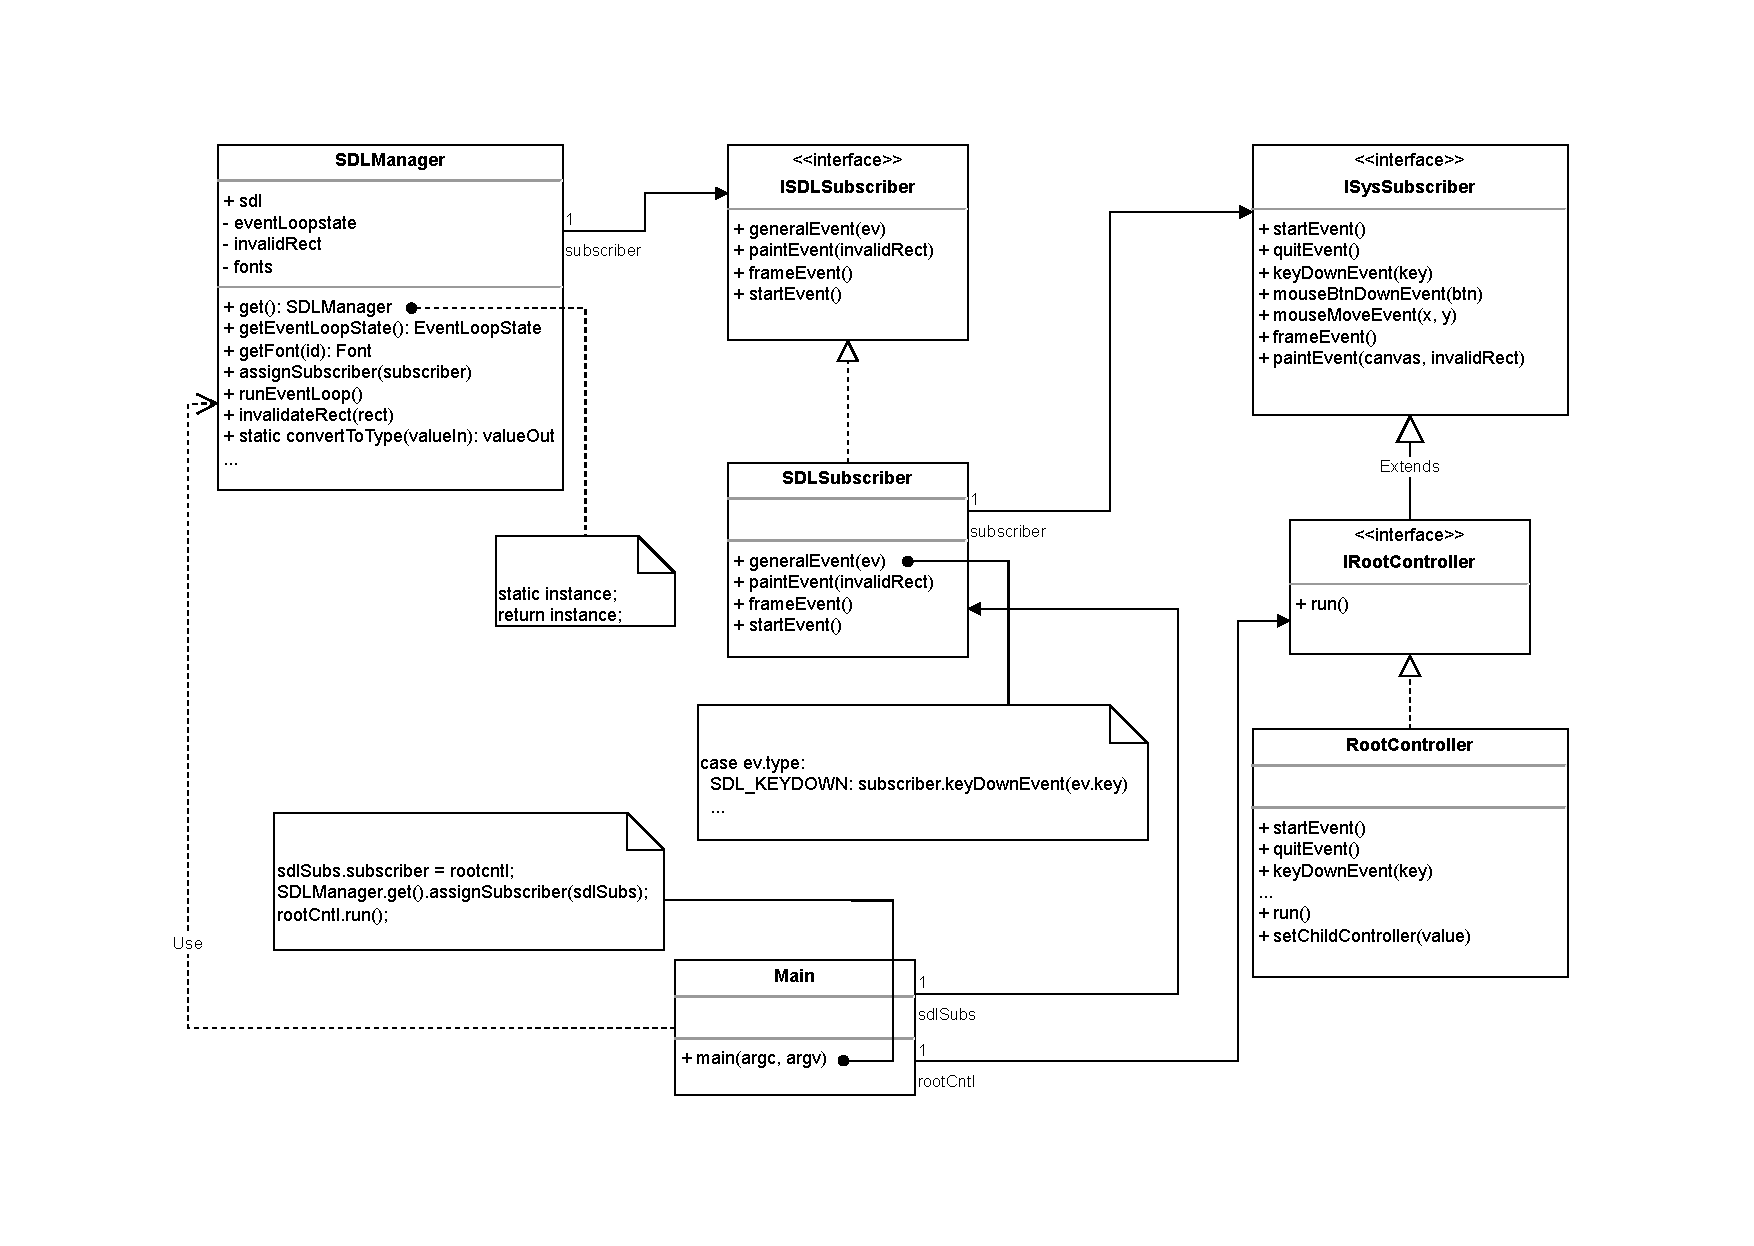
\includepdf[pages=-]{class-diagram.pdf}


% \chapter{Důkaz nekonečnosti stavového prostoru hry Bubble Brawl}
% \label{app:dukaz-nekonecnosti}

% Tato příloha dokazuje, že existuje nekonečně mnoho stavů, jakých může hra \emph{Bubble Brawl} nabývat. Důkaz se vztahuje k~jednomu hráči na herní ploše, jejíž rozměry jsou celá kladná (konečná) čísla, přičemž hráč \emph{nemění svoji velikost}. Výchozí stav hry je následující:
% \begin{itemize}
%     \item Na souřadnicích $[-50, -50]$ se nachází stěna překážky. Tato stěna pokračuje kolmo směrem dolů.
%     \item Na souřadnicích $[51 + \sqrt{2}, -50]$ se nachází jiná stěna překážky, která taktéž pokračuje kolmo směrem dolů.
%     \item Na souřadnicích $[0, 0]$ se nachází hráč, který má množství života stejné, jako na začátku hry.
%     \item Mezi těmito dvěma stěnami se nenachází žádní další hráči ani bonusy.
%     \item Šířka herní plochy je dostatečně velká, aby se do ní vlezly tyto 2 překážky. Výška herní plochy je dostatečně velká, aby se do ní vlezl hráč a~pod sebou měl alespoň $(1 + \sqrt{2}) + \frac{17}{6}$ místa.
% \end{itemize}
% Pro jednoduchost se uvažuje soustava souřadnic, jejíž souřadnice X roste směrem vpravo, souřadnice Y směrem dolů a~počátek soustavy je v~bodě, kde se nachází hráč. Stav hry je zobrazen na obrázku~\ref{fig:wa-bfs-predator-infinite}.

% \begin{figure}[ht]
%     \centering
%     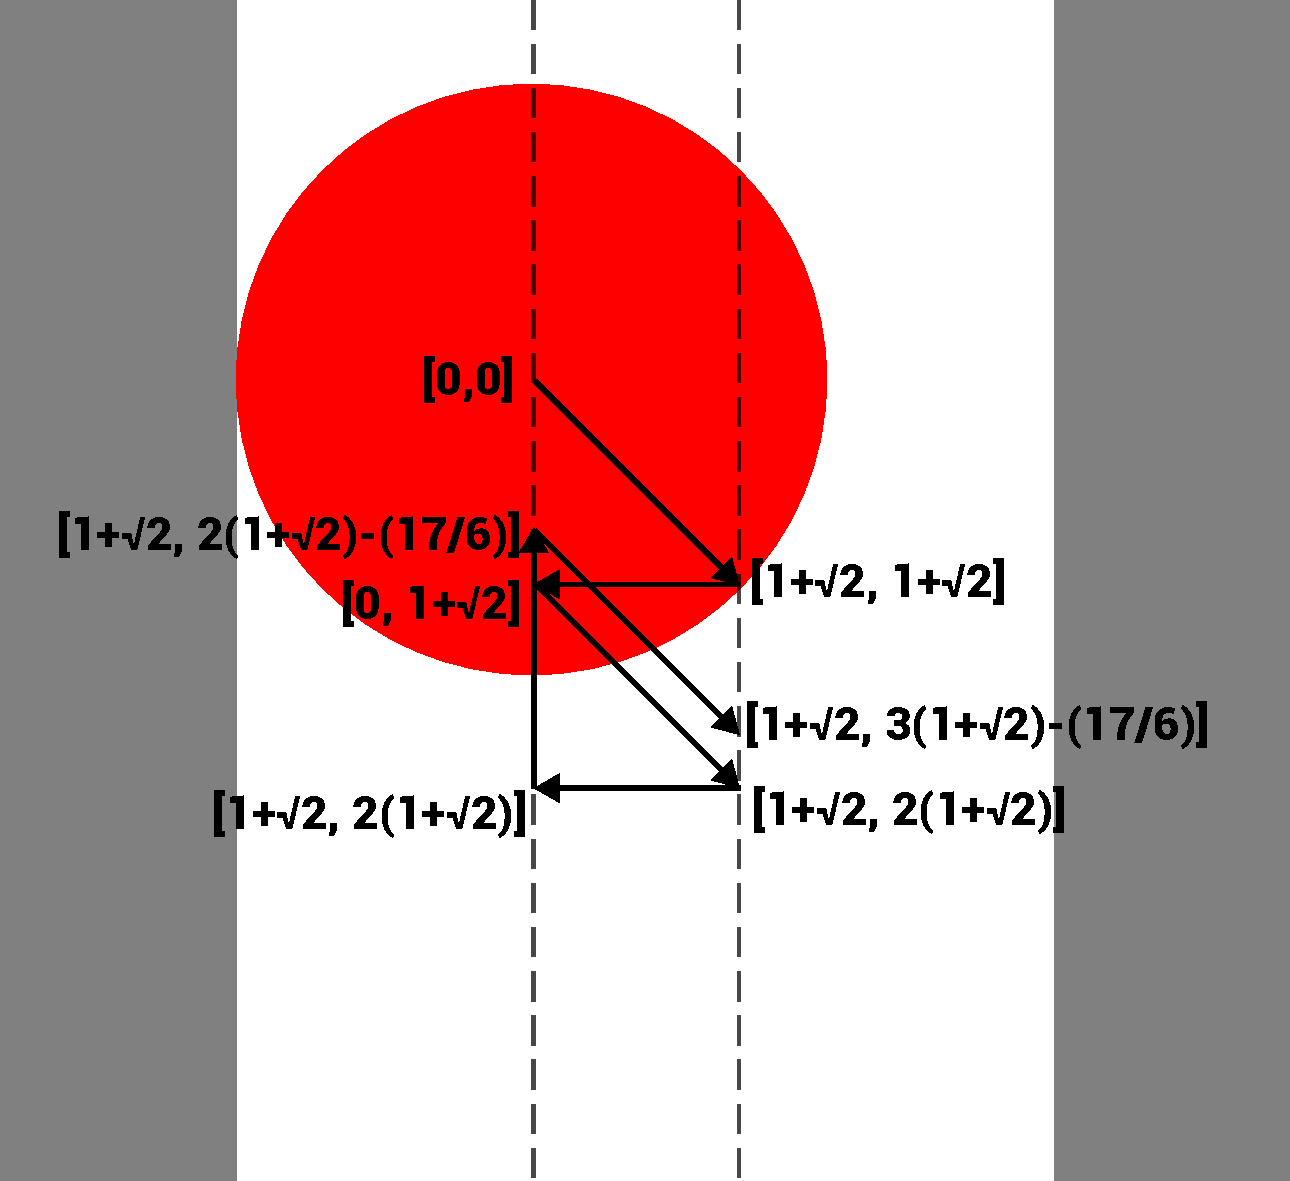
\includegraphics[width=0.8\textwidth]{doc/obrazky-figures/wa-bfs-predator-infinite.pdf}
%     \caption{Stav hry použitý pro důkaz. Černé šipky znázorňují pohyb hráče.}
%     \label{fig:wa-bfs-predator-infinite}
% \end{figure}

% Aby byl stavový prostor nekonečný, musí existovat nekonečná posloupnost kroků bez opakujících se stavů. Důkaz bude proveden sporem.

% Mějme tedy posloupnost stavů $(a_n)_{n = 1}^\infty$ generovanou tímto předpisem:
% \begin{equation}
%     (a_n)_{n = 1}^\infty,\quad a_n = \left\{\begin{array}{ll}
%         [0, 0] & \text{pro} n = 1 \\
%         a_{n-1} - (1 + \sqrt{2}, 0) & 
%     \end{array}\right.
% \end{equation}
% \begin{itemize}
%     \item pokud souřadnice X hráče není 0, a~tedy se dotýká pravé stěny, provede se pohyb vlevo. Jinak,
%     \item pokud je souřadnice Y hráče menší než $\frac{17}{6}$, provede se diagonální pohyb dolů doprava. Pozice hráče se tímto změní o~$(1 + \sqrt{2}, 1 + \sqrt{2})$. Jinak,
%     \item provede se pohyb nahoru. Pozice hráče se tímto změní o~$(0, \frac{17}{6})$.
% \end{itemize}
% Tato posloupnost je zobrazena na obrázku~\ref{fig:wa-bfs-predator-infinite}. Nyní předpokládejme, že tato posloupnost nekonečná \emph{není}. V~tom případě v~této posloupnosti existují 2~shodné stavy.


% \chapter{Algoritmus pro výpočet trajektorií hráčů}
% \label{app:vypocet-trajektorii-hracu}

% V~této příloze je popsán nepoužitý algoritmus pro výpočet trajektorií pohybu hráčů. Tento algoritmus nebyl použit, protože se nepovedlo přijít s~implementací, která by byla dostatečně výkonná. Nicméně je zde uveden pro případ, kdyby se povedlo výkon algoritmu optimalizovat.

% Algoritmus se snaží na herní ploše simulovat působení sil na entity hráčů. Stisk klávesy simuluje sílu působící na entitu požadovaným směrem. Při kolizi s~překážkou na entitu působí síla kolmá k~povrchu překážky. Tím pádem při nárazu do překážky entita dále pokračuje v~pohybu podél překážky, avšak s~menší rychlostí, a~pohyb tak působí přirozeně.

% \begin{figure}[ht]
%     \centering
%     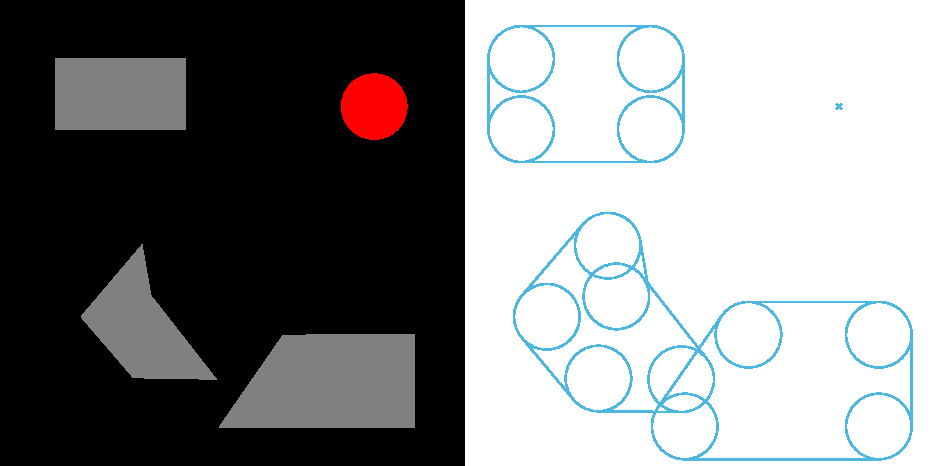
\includegraphics[width=0.9\textwidth]{doc/obrazky-figures/stage-logical.pdf}
%     \caption{Interní reprezentace herní plochy pro hledání kolizí s~překážkami. Vlevo je ukázka herní plochy tak, jak je prezentována uživateli, vpravo je převedena na interní reprezentaci.}
%     \label{fig:stage-logical}
% \end{figure}

% Algoritmus si interně vytváří model plochy, který se liší od způsobu, jakým je plocha prezentována na obrazovce. Zatímco překážky jsou vykreslovány jako mnohoúhelníky a~entity hráčů jako kruhy, interně jsou tyto tvary upraveny tak, aby se s~nimi lépe pracovalo. Všechny překážky jsou nejdříve upraveny tak, aby jejich vrcholy byly uspořádány proti směru hodinových ručiček. Stěny překážek jsou posunuty o~vzdálenost rovnu poloměru kruhu entity hráče, ve směru kolmém k této stěně. Rohy překážek ze změní v~kružnice se středem v~daném rohu a~poloměru stejném jako má entita hráče. Pak entita samotná se změní na pouhý bod v~rovině, který leží na stejných souřadnicích, jako střed kruhu entity hráče. Ukázka tohoto interního modelu je na obrázku~\ref{fig:stage-logical}.

% V~algoritmu je použito několik datových struktur. Jelikož algoritmus pracuje ve velké míře s~výpočty z~oblasti analytické a~výpočetní geometrie, mezi použité struktury patří \emph{bod}, \emph{vektor}, \emph{přímka}, \emph{úsečka}, \emph{kružnice} a~\emph{kruhový oblouk}. Krajní body \emph{úsečky} i~\emph{kruhového oblouku} jsou uspořádané, tedy jeden z~nich je vždy \emph{počáteční} a~druhý \emph{koncový}. \emph{Kruhový oblouk} může mít maximálně $180^\circ$ (avšak v~praxi nikdy nepřesáhne $90^\circ$). Další strukturou je \emph{úsek trajektorie}, který představuje buď \emph{úsečku}, nebo \emph{kruhový oblouk} (možná implementace v~jazyce \emph{C} by byla pomocí \emph{unie}). Také \emph{kolize s~překážkou} nebo \emph{hráč} jsou datové struktury. Jaké členy tyto struktury obsahují by mělo být zřejmé z~popisu algoritmu.

% Algoritmus dále pracuje s několika proměnnými:
% \begin{itemize}
%     \item $Traj$\,--\,seznam úseků trajektorie, představující celou trajektorii hráče,
%     \item $Tail$\,--\,zbývající úsek trajektorie po opuštění kolizní zóny s~překážkou (viz obrázek~\ref{fig:traj-tail}),
%     \item $MoveEnd$\,--\,přímka; hranice, kde končí hráčův pohyb,
%     \item $Flexible$\,--\,ohebnost posledního úseku trajektorie proměnné $Traj$. Může nabývat hodnot $CW$ (po směru hodinových ručiček\,--\,\emph{clockwise}), $CCW$ (proti směru hodinových ručiček\,--\,\emph{counterclockwise}) nebo $BOTH$ (ohebnost oběma směry), viz obázek~\ref{fig:flexible-both-cw},
%     \item $Coll$\,--\,informace o~poslední nalezené kolizi.
% \end{itemize}

% \begin{figure}[ht]
%     \centering
%     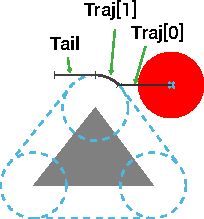
\includegraphics{doc/obrazky-figures/traj-tail.pdf}
%     \caption{Stav proměnných $Traj$ a~$Tail$ po vyhodnocení kolize s~rohem překážky. Při další iteraci hledání kolizí se z~$Tail$ stane $Traj[2]$.}
%     \label{fig:traj-tail}
% \end{figure}

% \begin{figure}[ht]
%     \centering
%     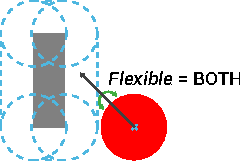
\includegraphics{doc/obrazky-figures/flexible-both.pdf}
%     \hspace{1cm}
%     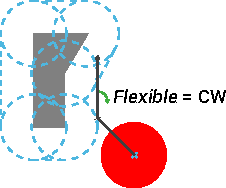
\includegraphics{doc/obrazky-figures/flexible-cw.pdf}
%     \caption{Hodnota proměnné $Flexible$ ve vztahu k~vybraným úsekům trajektorie. Vlevo je úsek ohebný oběma směry, vpravo pouze jedním směrem\,--\,po směru hodinových ručiček (\emph{clockwise}, \emph{CW}). Ohebnost úseku je v~obou případech také znázorněna zelenou šipkou.}
%     \label{fig:flexible-both-cw}
% \end{figure}

% Následuje samotný algoritmus popsaný sekvencí kroků. Jelikož tento algoritmus obsahuje poměrně velké množství kroků, byl rozdělen na několik částí. V~některých částech jsou některé kroky uzavřeny v~kulatých závorkách, což značí, že daný krok má být dále rozvinut v~jiné části algoritmu.

% \begin{enumerate}
%     \item Inicializuj:
%     \begin{itemize}
%         \item $Segment0$ jako úsek trajektorie představující požadovaný hráčův pohyb (úsečka vedoucí od aktuální pozice hráče ke koncovému bodu hráčova pohybu),
%         \item $Traj$ jako seznam obsahující pouze 1 položku\,--\,$Segment0$,
%         \item $Tail$ bez hodnoty,
%         \item $MoveEnd$ jako přímku kolmou na vektor hráčova pohybu, procházející bodem, kde končí hráčův pohyb,
%         \item $Flexible$ hodnotou $BOTH$ (ohebnost oběma směry).
%     \end{itemize}
%     \item \label{itm:trajectory-algo-1:begin-loop} Najdi kolizi $Coll$ posledního prvku seznamu $Traj$ s~překážkami.
%     \item Pokud nebyla nalezena žádná kolize, pak:
%     \begin{enumerate}
%         \item Pokud proměnná $Tail$ neobsahuje žádnou hodnotu, vrať $Traj$ jako výsledek; algoritmus končí.
%         \item Pokud proměnná $Tail$ obsahuje hodnotu (úsek trajektorie), připoj tuto hodnotu na konec seznamu $Traj$, nastav $Flexible$ na $BOTH$ a~vrať se na bod~\ref{itm:trajectory-algo-1:begin-loop}. Jinak pokračuj.
%     \end{enumerate}
%     \item \label{itm:trajectory-algo-1:call-process-coll} (Uprav hodnoty proměnných podle nalezené kolize $Coll$.)
%     \item Vrať se na bod~\ref{itm:trajectory-algo-1:begin-loop}.
% \end{enumerate}

% Výše je popsána základní část algoritmu, v~níž je provedena inicializace proměnných a~za ní následuje cyklus hledání kolizí. Je důležité si ujasnit, co je vnímáno jako \emph{kolize}: je to situace, kdy se kruh hráče překrývá s~překážkou. To znamená, že pokud se hráč pohybuje podél zdi nebo jeho pohyb končí nebo začíná těsně vedle zdi (přičemž během pohybu nedošlo k~překrytí s~překážkou), jedná se pouze o~\emph{dotek}, a~nikoliv o~\emph{kolizi}.

% Následuje část algoritmu vzniklá rozvinutím bodu~\ref{itm:trajectory-algo-1:call-process-coll} v~části algoritmu popsané výše:
% \begin{enumerate}
%     \item Nastav proměnnou $Tail$ do stavu bez hodnoty.
%     \item Nastav \emph{koncový bod} posledního prvku seznamu $Traj$ do bodu, kde nastala kolize.
%     \item Inicializuj nový úsek trajektorie $NewSegment$ podle kolize:
%     \begin{enumerate}
%         \item Pokud kolize nastala se stěnou překážky, pak $NewSegment$ bude \emph{úsečka}.
%         \item Pokud kolize nastala s~rohem překážky, pak $NewSegment$ bude \emph{kruhový oblouk} se středem stejným, jako je střed tohoto rohu.
%         \item \emph{Počáteční bod} bude v~obou případech v~bodě kolize. \emph{Koncový bod} zatím není znám.
%     \end{enumerate}
%     \item Urči přímku $Refl$, která je tečnou překážky v~bodě kolize.
%     \item Pokud je přímka $Refl$ kolmá na vektor hráčova pohybu, nastav koncový bod úseku $NewSegment$ do bodu kolize (bude to segment s~nulovou délkou), připoj jej na konec $Traj$ a~vrať $Traj$ jako výsledek; algoritmus končí (jedná se o~přímý náraz do překážky). Jinak pokračuj.
%     \item \label{itm:trajectory-algo-2:newsegment-flex} Urči ohebnost úseku $NewSegment$.
%     \item Pokud ohebnost úseku $NewSegment$ neodpovídá ohebnosti $Flexible$ (jsou různé a~zároveň $Flexible$ není $BOTH$), nastav koncový bod úseku $NewSegment$ do bodu kolize (bude to segment s~nulovou délkou), připoj jej na konec $Traj$ a~vrať $Traj$ jako výsledek; algoritmus končí (hráč se snaží projít příliš úzkým průchodem mezi překážkami). Jinak pokračuj.
%     \item Přepiš $Flexible$ hodnotou ohebnosti úseku $NewSegment$.
%     \item \label{itm:trajectory-algo-2:call-newsegment-endpoint} (Najdi \emph{koncový bod} úseku $NewSegment$.)
% \end{enumerate}

% Ohebnost úseku $NewSegment$ (bodě~\ref{itm:trajectory-algo-2:newsegment-flex}) se určí podle vztahu mezi vektorem pohybu hráče a~překážkou, jak je naznačeno na obrázku~\ref{fig:newsegment-wall-corner-flexible}. Pokud kolize nastala se stěnou překážky a~vektor pohybu hráče s~vektorem stěny svírají ostrý úhel (vektorem stěny je vektor z~\emph{počátečního} do \emph{koncového bodu} stěny), ohebnost je $CW$ (po směru hodinových ručiček). Pokud svírají tupý úhel, ohebnost je $CCW$ (proti směru hodinových ručiček). V~případě kolize s~rohem překážky 

% \begin{figure}
%     \centering
%     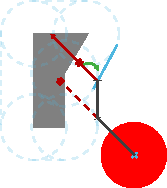
\includegraphics{doc/obrazky-figures/newsegment-wall-flexible.pdf}
%     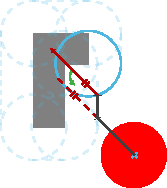
\includegraphics{doc/obrazky-figures/newsegment-corner-flexible.pdf}
%     \caption{Určení ohebnosti nového úseku trajektorie. Černá lomená čára ukazuje trajektorii pohybu hráče, červená šipka směr hráčova pohybu, zelená určenou ohebnost.}
%     \label{fig:newsegment-wall-corner-flexible}
% \end{figure}

% Další strukturou je úsek trajektorie, který představuje buď úsečku, nebo kruhový oblouk. Také na entitu hráče se nahlíží jako na datovou strukturu skládající se z~bodu, ve kterém se hráč nachází, a~vektoru hráčova pohybu.

% Níže je popsána procedura \textsc{Initialize}, která nastavuje výchozí hodnoty proměnných. Za zmínku stojí způsob, jakým je inicializována přímka $MoveEnd$ na řádku~\ref{alg:traj_old:line:init_MoveEnd}. Nezáleží totiž na její směrnici; přímka pouze nesmí být rovnoběžná s~vektorem pohybu hráče a~musí procházet bodem $MoveEndPt$. V~hlavním těle algoritmu bude počítán průsečík této přímky s~přímkou, po níž se pohybuje hráč, a~je nezbytně nutné, aby tento průsečík ležel právě v~bodě $MoveEndPt$.

% \begin{minipage}{\textwidth}
% \begin{algorithmic}[1]
%     \Procedure{Initialize}{$Traj$, $Tail$, $MoveEnd$, $Flexible$}
%         \State $Traj \gets \emptyset$
%         \State $Tail \gets NULL$
%         \State $MoveEndPt \gets Player.Position + Player.MovementVector$
%         \State $MoveEnd \gets$ \Call{Line}{$MoveEnd \perp Player.MovementVector \wedge MoveEndPt \in MoveEnd$} \label{alg:traj_old:line:init_MoveEnd}
%         \State $Flexible \gets BOTH$
%         \State $Segment0.Type \gets LINE\_SEGMENT$
%         \State $Segment0.PStart \gets Player.Position$
%         \State $Segment0.PEnd \gets MoveEndPt$
%         \State $Traj.$\Call{Push}{$Segment0$}
%     \EndProcedure
% \end{algorithmic}
% \end{minipage}

% \begin{minipage}{\textwidth}
% \begin{algorithmic}[1]
%     \Procedure{Main}{}
%         \State \Call{Initialize}{$Traj$, $Tail$, $MoveEnd$, $Flexible$}
%         \Loop
%             \State find the nearest $Collision$ of $Traj.Last$ with obstacles
%             \If{no $Collision$ was found}
%                 \If{$Tail = NULL$}
%                     \State \Return $Traj$
%                 \Else
%                     \State $Traj.$\Call{Push}{$Tail$}
%                     \State $Flexible \gets BOTH$
%                     \State $Tail \gets NULL$
%                 \EndIf
%             \Else
%             \EndIf
%         \EndLoop
%     \EndProcedure
% \end{algorithmic}
% \end{minipage}


% Pro kompilaci po částech (viz projekt.tex) nutno odkomentovat
%\end{document}

  \fi
  
  % Kompilace po částech (viz výše, nutno odkomentovat)
  % Compilation piecewise (see above, it is necessary to uncomment it)
  %\subfile{projekt-30-prilohy-appendices}
  
\end{document}
